% =====================================================================
%  Fondamenti di Unreal Engine, lezione 13 — Introduzione al level
%  design: la gym, il block out con le geometry brush e le luci.
%  Tredicesima lezione del corso breve di introduzione a Unreal Engine,
%  la prima delle "ultime quattro lezioni" con il nuovo docente,
%  dedicate al level design. Lezione online (Zoom), di giovedì
%  pomeriggio: inizio alle 16:10, pausa alle 17:30 con ripresa alle
%  17:45, chiusura poco dopo le 19. Il docente non dice mai il proprio
%  nome nella trascrizione; le lezioni precedenti annunciavano che il
%  corso sarebbe proseguito con Davide e il level design, e il docente
%  nomina Igor (il docente delle lezioni 1-12) come collega: con ogni
%  probabilità è Davide (il capitolo lo dichiara come deduzione).
%  Contenuti, nell'ordine della lezione: l'apertura (i problemi di
%  audio e di caldo, il programma delle quattro lezioni: teoria, block
%  out e geometry brush, forse il modeling mode, Landscape e Foliage
%  Mode, luci, post produzione, dressing, l'esercitazione finale con gli
%  eseguibili sul Discord); da dove si parte (la realtà o un altro
%  gioco: Spider-Man e Manhattan, Assassin's Creed Brotherhood e
%  l'acqua, le meccaniche fatte con Igor); il level design document; il
%  layout (la piantina numerata, il platform 2D a quadretti, la mappa di
%  un metroidvania); la gym o test level (altezze di salto, porte e
%  camera in terza persona, wall run, angolo camminabile, altezza da
%  accovacciati); il block out (il case study del block out di God of
%  War 2018, i landmark, il forziere, la catena, le bandiere); in
%  engine: la gym abbozzata con le meccaniche di Igor, il materiale a
%  griglia e lo snapping, la Max Sprint Distance di 26 m e i suoi usi
%  (inseguimento, ricariche di stamina, horror); i blocchi da 1 a 2 m e
%  il feeling del salto (la capsula); il Character Movement (Gravity
%  Scale, Mass, Max Step Height, Walkable Floor Angle, Max Walk Speed,
%  crouch, Jump Z Velocity da 420 a 700, Air Control, Falling Friction,
%  nuoto e volo), le misure del salto (4 m camminando, 6 m correndo);
%  le geometry brush (static mesh contro brush, Unreal 4 e il modeling
%  tool, il menu Quick Add e il Place Actors Panel, i materiali per
%  faccia, Brush Settings al posto della scala, Box, Hollow, Wall
%  Thickness, Tessellated, Additive e Subtractive, Create Static Mesh e
%  la cartella dei blockout asset, Cone, Cylinder, Sphere, le tre
%  scale, il Brush Editing mode e lo Split); la pausa e la scelta del
%  formato delle lezioni; le luci (i cinque tipi, la Mobility static,
%  stationary e movable, la Directional Light, Intensity, Light Color e
%  Hex Linear, Temperature, Affects World, Cast Shadows, Dynamic Shadow
%  Distance, una sola directional e una sola sky light, la Sky Light e
%  l'ambient occlusion, point light contro spot light, l'Attenuation
%  Radius, la X rossa delle ombre, il corridoio, Source Radius, Soft
%  Source Radius e Source Length, i neon, la spot light e i coni, la
%  domanda sull'effetto accecante e il post process, la Rect Light e le
%  Barn Door, il build delle luci e le qualità, Unreal 4 e "Lighting
%  needs to be rebuilt", le Reflection Capture e i materiali
%  riflettenti); i compiti per martedì (gym, parametri del bot,
%  block out con 3-5 collezionabili); la chiusura.
%  Fonte: trascrizione automatica della tredicesima lezione (UE13).
%  Integrazioni dal libro "Blueprints Visual Scripting for Unreal Engine 5"
%  (Romero, Sewell; capitoli 3, 4, 6, 9, 12 e 13) e da "An Architectural
%  Approach to Level Design" (Totten; capitolo 2 e capitolo sulle
%  strutture dei mondi di gioco), entrambi nella cartella Libri del
%  progetto, e nozioni tecniche generali su Unreal Engine 5, sempre
%  segnalate come approfondimenti. Il libro di Romero e Sewell non
%  tratta le geometry brush, la Mobility delle luci in dettaglio, il
%  build delle luci, le Reflection Capture, la X rossa delle luci
%  stazionarie né i parametri del salto del Character Movement: su
%  questi argomenti gli approfondimenti si basano sul funzionamento
%  generale dell'engine.
%
%  Pacchetti richiesti nel preambolo del libro (già presenti nel
%  main.tex): \usepackage{booktabs}, \usepackage{amsmath},
%  \usepackage{amssymb}, \usepackage{tikz} con
%    \usetikzlibrary{shapes.geometric,shapes.symbols,shapes.misc,
%      arrows.meta,positioning,calc,fit}
%  (le librerie vanno caricate nel preambolo, non nel capitolo).
%  Consigliati, come per gli altri capitoli: \usepackage[italian]{babel}
%  e \usepackage[T1]{fontenc} (il capitolo compila anche senza).
%
%  Collocazione nel libro: parte "Fondamenti di Unreal Engine",
%  tredicesimo capitolo (numerazione propria 1.13). Nel file principale
%  del libro, subito dopo la riga della dodicesima lezione:
%
%    % =====================================================================
%  Fondamenti di Unreal Engine, lezione 13 — Introduzione al level
%  design: la gym, il block out con le geometry brush e le luci.
%  Tredicesima lezione del corso breve di introduzione a Unreal Engine,
%  la prima delle "ultime quattro lezioni" con il nuovo docente,
%  dedicate al level design. Lezione online (Zoom), di giovedì
%  pomeriggio: inizio alle 16:10, pausa alle 17:30 con ripresa alle
%  17:45, chiusura poco dopo le 19. Il docente non dice mai il proprio
%  nome nella trascrizione; le lezioni precedenti annunciavano che il
%  corso sarebbe proseguito con Davide e il level design, e il docente
%  nomina Igor (il docente delle lezioni 1-12) come collega: con ogni
%  probabilità è Davide (il capitolo lo dichiara come deduzione).
%  Contenuti, nell'ordine della lezione: l'apertura (i problemi di
%  audio e di caldo, il programma delle quattro lezioni: teoria, block
%  out e geometry brush, forse il modeling mode, Landscape e Foliage
%  Mode, luci, post produzione, dressing, l'esercitazione finale con gli
%  eseguibili sul Discord); da dove si parte (la realtà o un altro
%  gioco: Spider-Man e Manhattan, Assassin's Creed Brotherhood e
%  l'acqua, le meccaniche fatte con Igor); il level design document; il
%  layout (la piantina numerata, il platform 2D a quadretti, la mappa di
%  un metroidvania); la gym o test level (altezze di salto, porte e
%  camera in terza persona, wall run, angolo camminabile, altezza da
%  accovacciati); il block out (il case study del block out di God of
%  War 2018, i landmark, il forziere, la catena, le bandiere); in
%  engine: la gym abbozzata con le meccaniche di Igor, il materiale a
%  griglia e lo snapping, la Max Sprint Distance di 26 m e i suoi usi
%  (inseguimento, ricariche di stamina, horror); i blocchi da 1 a 2 m e
%  il feeling del salto (la capsula); il Character Movement (Gravity
%  Scale, Mass, Max Step Height, Walkable Floor Angle, Max Walk Speed,
%  crouch, Jump Z Velocity da 420 a 700, Air Control, Falling Friction,
%  nuoto e volo), le misure del salto (4 m camminando, 6 m correndo);
%  le geometry brush (static mesh contro brush, Unreal 4 e il modeling
%  tool, il menu Quick Add e il Place Actors Panel, i materiali per
%  faccia, Brush Settings al posto della scala, Box, Hollow, Wall
%  Thickness, Tessellated, Additive e Subtractive, Create Static Mesh e
%  la cartella dei blockout asset, Cone, Cylinder, Sphere, le tre
%  scale, il Brush Editing mode e lo Split); la pausa e la scelta del
%  formato delle lezioni; le luci (i cinque tipi, la Mobility static,
%  stationary e movable, la Directional Light, Intensity, Light Color e
%  Hex Linear, Temperature, Affects World, Cast Shadows, Dynamic Shadow
%  Distance, una sola directional e una sola sky light, la Sky Light e
%  l'ambient occlusion, point light contro spot light, l'Attenuation
%  Radius, la X rossa delle ombre, il corridoio, Source Radius, Soft
%  Source Radius e Source Length, i neon, la spot light e i coni, la
%  domanda sull'effetto accecante e il post process, la Rect Light e le
%  Barn Door, il build delle luci e le qualità, Unreal 4 e "Lighting
%  needs to be rebuilt", le Reflection Capture e i materiali
%  riflettenti); i compiti per martedì (gym, parametri del bot,
%  block out con 3-5 collezionabili); la chiusura.
%  Fonte: trascrizione automatica della tredicesima lezione (UE13).
%  Integrazioni dal libro "Blueprints Visual Scripting for Unreal Engine 5"
%  (Romero, Sewell; capitoli 3, 4, 6, 9, 12 e 13) e da "An Architectural
%  Approach to Level Design" (Totten; capitolo 2 e capitolo sulle
%  strutture dei mondi di gioco), entrambi nella cartella Libri del
%  progetto, e nozioni tecniche generali su Unreal Engine 5, sempre
%  segnalate come approfondimenti. Il libro di Romero e Sewell non
%  tratta le geometry brush, la Mobility delle luci in dettaglio, il
%  build delle luci, le Reflection Capture, la X rossa delle luci
%  stazionarie né i parametri del salto del Character Movement: su
%  questi argomenti gli approfondimenti si basano sul funzionamento
%  generale dell'engine.
%
%  Pacchetti richiesti nel preambolo del libro (già presenti nel
%  main.tex): \usepackage{booktabs}, \usepackage{amsmath},
%  \usepackage{amssymb}, \usepackage{tikz} con
%    \usetikzlibrary{shapes.geometric,shapes.symbols,shapes.misc,
%      arrows.meta,positioning,calc,fit}
%  (le librerie vanno caricate nel preambolo, non nel capitolo).
%  Consigliati, come per gli altri capitoli: \usepackage[italian]{babel}
%  e \usepackage[T1]{fontenc} (il capitolo compila anche senza).
%
%  Collocazione nel libro: parte "Fondamenti di Unreal Engine",
%  tredicesimo capitolo (numerazione propria 1.13). Nel file principale
%  del libro, subito dopo la riga della dodicesima lezione:
%
%    % =====================================================================
%  Fondamenti di Unreal Engine, lezione 13 — Introduzione al level
%  design: la gym, il block out con le geometry brush e le luci.
%  Tredicesima lezione del corso breve di introduzione a Unreal Engine,
%  la prima delle "ultime quattro lezioni" con il nuovo docente,
%  dedicate al level design. Lezione online (Zoom), di giovedì
%  pomeriggio: inizio alle 16:10, pausa alle 17:30 con ripresa alle
%  17:45, chiusura poco dopo le 19. Il docente non dice mai il proprio
%  nome nella trascrizione; le lezioni precedenti annunciavano che il
%  corso sarebbe proseguito con Davide e il level design, e il docente
%  nomina Igor (il docente delle lezioni 1-12) come collega: con ogni
%  probabilità è Davide (il capitolo lo dichiara come deduzione).
%  Contenuti, nell'ordine della lezione: l'apertura (i problemi di
%  audio e di caldo, il programma delle quattro lezioni: teoria, block
%  out e geometry brush, forse il modeling mode, Landscape e Foliage
%  Mode, luci, post produzione, dressing, l'esercitazione finale con gli
%  eseguibili sul Discord); da dove si parte (la realtà o un altro
%  gioco: Spider-Man e Manhattan, Assassin's Creed Brotherhood e
%  l'acqua, le meccaniche fatte con Igor); il level design document; il
%  layout (la piantina numerata, il platform 2D a quadretti, la mappa di
%  un metroidvania); la gym o test level (altezze di salto, porte e
%  camera in terza persona, wall run, angolo camminabile, altezza da
%  accovacciati); il block out (il case study del block out di God of
%  War 2018, i landmark, il forziere, la catena, le bandiere); in
%  engine: la gym abbozzata con le meccaniche di Igor, il materiale a
%  griglia e lo snapping, la Max Sprint Distance di 26 m e i suoi usi
%  (inseguimento, ricariche di stamina, horror); i blocchi da 1 a 2 m e
%  il feeling del salto (la capsula); il Character Movement (Gravity
%  Scale, Mass, Max Step Height, Walkable Floor Angle, Max Walk Speed,
%  crouch, Jump Z Velocity da 420 a 700, Air Control, Falling Friction,
%  nuoto e volo), le misure del salto (4 m camminando, 6 m correndo);
%  le geometry brush (static mesh contro brush, Unreal 4 e il modeling
%  tool, il menu Quick Add e il Place Actors Panel, i materiali per
%  faccia, Brush Settings al posto della scala, Box, Hollow, Wall
%  Thickness, Tessellated, Additive e Subtractive, Create Static Mesh e
%  la cartella dei blockout asset, Cone, Cylinder, Sphere, le tre
%  scale, il Brush Editing mode e lo Split); la pausa e la scelta del
%  formato delle lezioni; le luci (i cinque tipi, la Mobility static,
%  stationary e movable, la Directional Light, Intensity, Light Color e
%  Hex Linear, Temperature, Affects World, Cast Shadows, Dynamic Shadow
%  Distance, una sola directional e una sola sky light, la Sky Light e
%  l'ambient occlusion, point light contro spot light, l'Attenuation
%  Radius, la X rossa delle ombre, il corridoio, Source Radius, Soft
%  Source Radius e Source Length, i neon, la spot light e i coni, la
%  domanda sull'effetto accecante e il post process, la Rect Light e le
%  Barn Door, il build delle luci e le qualità, Unreal 4 e "Lighting
%  needs to be rebuilt", le Reflection Capture e i materiali
%  riflettenti); i compiti per martedì (gym, parametri del bot,
%  block out con 3-5 collezionabili); la chiusura.
%  Fonte: trascrizione automatica della tredicesima lezione (UE13).
%  Integrazioni dal libro "Blueprints Visual Scripting for Unreal Engine 5"
%  (Romero, Sewell; capitoli 3, 4, 6, 9, 12 e 13) e da "An Architectural
%  Approach to Level Design" (Totten; capitolo 2 e capitolo sulle
%  strutture dei mondi di gioco), entrambi nella cartella Libri del
%  progetto, e nozioni tecniche generali su Unreal Engine 5, sempre
%  segnalate come approfondimenti. Il libro di Romero e Sewell non
%  tratta le geometry brush, la Mobility delle luci in dettaglio, il
%  build delle luci, le Reflection Capture, la X rossa delle luci
%  stazionarie né i parametri del salto del Character Movement: su
%  questi argomenti gli approfondimenti si basano sul funzionamento
%  generale dell'engine.
%
%  Pacchetti richiesti nel preambolo del libro (già presenti nel
%  main.tex): \usepackage{booktabs}, \usepackage{amsmath},
%  \usepackage{amssymb}, \usepackage{tikz} con
%    \usetikzlibrary{shapes.geometric,shapes.symbols,shapes.misc,
%      arrows.meta,positioning,calc,fit}
%  (le librerie vanno caricate nel preambolo, non nel capitolo).
%  Consigliati, come per gli altri capitoli: \usepackage[italian]{babel}
%  e \usepackage[T1]{fontenc} (il capitolo compila anche senza).
%
%  Collocazione nel libro: parte "Fondamenti di Unreal Engine",
%  tredicesimo capitolo (numerazione propria 1.13). Nel file principale
%  del libro, subito dopo la riga della dodicesima lezione:
%
%    % =====================================================================
%  Fondamenti di Unreal Engine, lezione 13 — Introduzione al level
%  design: la gym, il block out con le geometry brush e le luci.
%  Tredicesima lezione del corso breve di introduzione a Unreal Engine,
%  la prima delle "ultime quattro lezioni" con il nuovo docente,
%  dedicate al level design. Lezione online (Zoom), di giovedì
%  pomeriggio: inizio alle 16:10, pausa alle 17:30 con ripresa alle
%  17:45, chiusura poco dopo le 19. Il docente non dice mai il proprio
%  nome nella trascrizione; le lezioni precedenti annunciavano che il
%  corso sarebbe proseguito con Davide e il level design, e il docente
%  nomina Igor (il docente delle lezioni 1-12) come collega: con ogni
%  probabilità è Davide (il capitolo lo dichiara come deduzione).
%  Contenuti, nell'ordine della lezione: l'apertura (i problemi di
%  audio e di caldo, il programma delle quattro lezioni: teoria, block
%  out e geometry brush, forse il modeling mode, Landscape e Foliage
%  Mode, luci, post produzione, dressing, l'esercitazione finale con gli
%  eseguibili sul Discord); da dove si parte (la realtà o un altro
%  gioco: Spider-Man e Manhattan, Assassin's Creed Brotherhood e
%  l'acqua, le meccaniche fatte con Igor); il level design document; il
%  layout (la piantina numerata, il platform 2D a quadretti, la mappa di
%  un metroidvania); la gym o test level (altezze di salto, porte e
%  camera in terza persona, wall run, angolo camminabile, altezza da
%  accovacciati); il block out (il case study del block out di God of
%  War 2018, i landmark, il forziere, la catena, le bandiere); in
%  engine: la gym abbozzata con le meccaniche di Igor, il materiale a
%  griglia e lo snapping, la Max Sprint Distance di 26 m e i suoi usi
%  (inseguimento, ricariche di stamina, horror); i blocchi da 1 a 2 m e
%  il feeling del salto (la capsula); il Character Movement (Gravity
%  Scale, Mass, Max Step Height, Walkable Floor Angle, Max Walk Speed,
%  crouch, Jump Z Velocity da 420 a 700, Air Control, Falling Friction,
%  nuoto e volo), le misure del salto (4 m camminando, 6 m correndo);
%  le geometry brush (static mesh contro brush, Unreal 4 e il modeling
%  tool, il menu Quick Add e il Place Actors Panel, i materiali per
%  faccia, Brush Settings al posto della scala, Box, Hollow, Wall
%  Thickness, Tessellated, Additive e Subtractive, Create Static Mesh e
%  la cartella dei blockout asset, Cone, Cylinder, Sphere, le tre
%  scale, il Brush Editing mode e lo Split); la pausa e la scelta del
%  formato delle lezioni; le luci (i cinque tipi, la Mobility static,
%  stationary e movable, la Directional Light, Intensity, Light Color e
%  Hex Linear, Temperature, Affects World, Cast Shadows, Dynamic Shadow
%  Distance, una sola directional e una sola sky light, la Sky Light e
%  l'ambient occlusion, point light contro spot light, l'Attenuation
%  Radius, la X rossa delle ombre, il corridoio, Source Radius, Soft
%  Source Radius e Source Length, i neon, la spot light e i coni, la
%  domanda sull'effetto accecante e il post process, la Rect Light e le
%  Barn Door, il build delle luci e le qualità, Unreal 4 e "Lighting
%  needs to be rebuilt", le Reflection Capture e i materiali
%  riflettenti); i compiti per martedì (gym, parametri del bot,
%  block out con 3-5 collezionabili); la chiusura.
%  Fonte: trascrizione automatica della tredicesima lezione (UE13).
%  Integrazioni dal libro "Blueprints Visual Scripting for Unreal Engine 5"
%  (Romero, Sewell; capitoli 3, 4, 6, 9, 12 e 13) e da "An Architectural
%  Approach to Level Design" (Totten; capitolo 2 e capitolo sulle
%  strutture dei mondi di gioco), entrambi nella cartella Libri del
%  progetto, e nozioni tecniche generali su Unreal Engine 5, sempre
%  segnalate come approfondimenti. Il libro di Romero e Sewell non
%  tratta le geometry brush, la Mobility delle luci in dettaglio, il
%  build delle luci, le Reflection Capture, la X rossa delle luci
%  stazionarie né i parametri del salto del Character Movement: su
%  questi argomenti gli approfondimenti si basano sul funzionamento
%  generale dell'engine.
%
%  Pacchetti richiesti nel preambolo del libro (già presenti nel
%  main.tex): \usepackage{booktabs}, \usepackage{amsmath},
%  \usepackage{amssymb}, \usepackage{tikz} con
%    \usetikzlibrary{shapes.geometric,shapes.symbols,shapes.misc,
%      arrows.meta,positioning,calc,fit}
%  (le librerie vanno caricate nel preambolo, non nel capitolo).
%  Consigliati, come per gli altri capitoli: \usepackage[italian]{babel}
%  e \usepackage[T1]{fontenc} (il capitolo compila anche senza).
%
%  Collocazione nel libro: parte "Fondamenti di Unreal Engine",
%  tredicesimo capitolo (numerazione propria 1.13). Nel file principale
%  del libro, subito dopo la riga della dodicesima lezione:
%
%    \input{UE/UE13_gym_blockout_e_luci}
%
%  Tutte le etichette di questo capitolo hanno il prefisso "ue13:"
%  (ue13:cap:..., ue13:sec:..., ue13:fig:..., ue13:tab:...), e tutti gli
%  stili TikZ hanno il prefisso "ue13" (ue13box, ue13room, ...) per non
%  collidere con chiavi native di TikZ né con quelli delle lezioni
%  precedenti. Il capitolo è autonomo: non contiene \ref verso altri
%  capitoli (i rimandi alle lezioni precedenti sono a parole). Le figure
%  sono ricostruzioni schematiche di quanto mostrato e detto a lezione
%  (le slide e il video non sono nella trascrizione), non copie delle
%  schermate del docente. Dove la trascrizione è troppo rovinata per
%  ricostruire un dettaglio, il capitolo lo dice invece di inventarlo.
% =====================================================================

\chapter[Gym, block out e luci]{Introduzione al level design: la gym, il block out
e le luci}
\label{ue13:cap:leveldesign}

Questa è la \textbf{tredicesima lezione} del corso breve di \textbf{introduzione a Unreal
Engine}, e la prima con un \textbf{nuovo docente}. Le dodici lezioni precedenti, con
\textbf{Igor}, hanno costruito un piccolo repertorio di meccaniche (il personaggio
\textbf{bot} che cammina, corre e salta, la stamina, i collezionabili, la torretta che
spara, le porte che si aprono, le pedane che salgono e scendono, la luce che si accende,
i materiali fisici dell'acqua e della roccia). Le ultime \textbf{quattro lezioni} cambiano
prospettiva: non più ``come si programma una meccanica'', ma \textbf{come si costruisce un
livello} che quelle meccaniche le metta alla prova. ``L'idea delle mie lezioni, di queste
mie ultime quattro lezioni, sarà quella di spiegare un po' il \emph{workflow} che c'è alla
base della creazione di un livello e iniziare a mettere su dei livellini.''

Il docente non dice mai il proprio nome nella trascrizione. Le lezioni precedenti
annunciavano che il corso sarebbe proseguito ``con Davide'' e con il \emph{level design}, e
qui il docente parla di Igor come di un collega (``io e Igor proviamo le cose che avete
fatto''): il docente è quindi, con ogni probabilità, \textbf{Davide}, ma è una deduzione del
capitolo, non qualcosa che la lezione dica. Nel resto del capitolo è semplicemente ``il
docente''.

La giornata ha tre parti. La prima è un ``filo di teoria'', ``niente di troppo pesante'':
da dove si prende l'ispirazione per un livello, il \textbf{level design document}, il
\textbf{layout} (la piantina), la \textbf{gym} (il livello di prova in cui si misurano le
capacità del personaggio) e il \textbf{block out} (il livello rifatto con sole geometrie).
La seconda è pratica, in Unreal: si abbozza una gym con il bot, si misurano la corsa e i
salti, si toccano i parametri del \textbf{Character Movement} e si conoscono le
\textbf{geometry brush}, lo strumento classico per fare un block out. La terza, dopo la
pausa, è una panoramica sulle \textbf{luci}: i tipi di luce di Unreal, la loro
\emph{mobility}, i parametri principali, il costo delle ombre, il \emph{build} delle luci e
le \emph{reflection capture}. In chiusura, il compito per la lezione successiva: una gym
propria e un piccolo block out con da tre a cinque collezionabili.

Tre avvertenze di lettura, come per le lezioni precedenti. La prima: la trascrizione è
automatica e storpia moltissimi nomi. Unreal è ``Real'', ``un reale'' e ``Arial''; la
\textbf{gym} è ``GIM'' e ``JIM''; il \textbf{block out} è una volta ``plot out'' e il
\emph{blockouting} ``lockout''; \textbf{Kratos} è ``Gratos'' e ``Grados''; la
\textbf{Max Sprint Distance} è ``Mazda Sprint'' e ``Max Print Distance''; il Blueprint del
bot, \textbf{BP\_Bot2} (``character bot 2''), è una volta ``bottegger''; il
\textbf{Walkable Floor Angle} è ``workable floor angle'' e ``Walk and roll Flow Rainbow'';
la \textbf{static mesh} è ``state mesh'' e ``state Mesh''; il \textbf{Foliage Mode} è
``Folliage Mode''; il \textbf{Light Color} è ``let color'' e ``LED color''; il codice
\textbf{Hex Linear} è ``l'ex liner'' e ``gli ex''; \textbf{Affects World} è ``FXWord'';
l'\textbf{ambient occlusion} è ``ambiente occlusion''; il \textbf{Source Radius} è ``la
sorsa'' e il \textbf{Soft Source Radius} ``SRADUS soft SRADUS''; la \textbf{Source Length}
è ``la lent''; le \textbf{Barn Door} sono ``bar and door''; la \textbf{Planar Reflection}
è ``Lanar Reflection Capture''; \emph{baked} (``cotto'', precalcolato) è reso con
``becata'', ``abbicata'', ``baicata'' e ``vacato''; \emph{Breaking Bad} è ``break in
bed''. Dove la ricostruzione è sicura il capitolo usa la forma corretta; dove non lo è
riporta la forma della trascrizione e lo dice. La seconda: in alcuni punti il
riconoscimento vocale produce testo estraneo alla lezione. In apertura ci sono frasi su
``la situazione interna a livello politico'' e su ``gli egiziani'', poco dopo una frase
ripetuta (``io personalmente sono a favore di questa cosa''), a metà della parte sulle
scale una serie di frasi senza senso (``non preoccupatevi se non mi ricordo bene le mie
relazioni'') e, durante la pausa, un lungo blocco ripetuto decine di volte (``grazie a
tutti per l'attenzione che ci ha spiegato'', ``qual è la risposta che ci può essere?''):
non appartengono alla lezione e sono stati ignorati. La terza: le slide e il video
mostrati dal docente non sono nella trascrizione; il capitolo ricostruisce le immagini da
ciò che il docente dice mentre le indica, completa i nomi esatti dei parametri di Unreal
Engine~5, distingue le prove dalle conclusioni e dichiara i punti in cui la trascrizione
lascia un buco.

\paragraph{Come leggere questo capitolo.} Il capitolo segue l'ordine della lezione. Le
figure ricostruiscono la mappa di un metroidvania commentata dal docente, il percorso a
quadretti di un platform, la gym costruita in diretta, il ``feeling'' dei due salti
provati, le brush additive e sottrattive, le tre \emph{mobility} delle luci e le forme
delle luci locali. Le tabelle riassumono le misure della giornata, i parametri del
Character Movement, i parametri delle brush e delle luci, i problemi incontrati e le
impostazioni usate. Qua e là, dei paragrafi di \textbf{approfondimento} collegano la
lezione al libro di Marcos Romero e Brenden Sewell, \emph{Blueprints Visual Scripting for
Unreal Engine 5}, il testo di riferimento per questa parte del libro, al libro di
Christopher W.\ Totten, \emph{An Architectural Approach to Level Design}, che tratta
proprio i temi teorici della giornata, e a qualche nozione tecnica generale su Unreal
Engine~5; sono segnalati come tali e non fanno parte della lezione.

Il percorso del capitolo:
\begin{enumerate}
  \item l'\textbf{apertura} e il programma delle ultime quattro lezioni
        (sezione~\ref{ue13:sec:apertura});
  \item \textbf{da dove si parte}: la realtà o un altro gioco
        (sezione~\ref{ue13:sec:ispirazione});
  \item il \textbf{level design document} e il \textbf{layout}
        (sezione~\ref{ue13:sec:layout});
  \item la \textbf{gym}, il livello di prova (sezione~\ref{ue13:sec:gym});
  \item il \textbf{block out} e il caso di God of War (sezione~\ref{ue13:sec:blockout});
  \item in engine: la gym, la griglia e la \textbf{distanza di sprint}
        (sezione~\ref{ue13:sec:sprint});
  \item i \textbf{salti} e il \emph{feeling} del personaggio
        (sezione~\ref{ue13:sec:salti});
  \item i parametri del \textbf{Character Movement} (sezione~\ref{ue13:sec:cmc});
  \item le \textbf{geometry brush} (sezioni \ref{ue13:sec:brush} e~\ref{ue13:sec:forme});
  \item la \textbf{pausa} e la scelta del formato delle lezioni
        (sezione~\ref{ue13:sec:pausa});
  \item le \textbf{luci}: tipi e \emph{mobility} (sezione~\ref{ue13:sec:mobility}),
        directional e sky light (sezione~\ref{ue13:sec:directional}), point e spot light
        (sezione~\ref{ue13:sec:point}), rect light (sezione~\ref{ue13:sec:rect}), il
        \emph{build} e i riflessi (sezione~\ref{ue13:sec:build});
  \item i \textbf{compiti} per martedì e la chiusura (sezione~\ref{ue13:sec:compiti}).
\end{enumerate}

% ---------------------------------------------------------------------
\section{L'apertura e il programma delle ultime quattro lezioni}
\label{ue13:sec:apertura}

\paragraph{L'audio e il caldo.} I primi minuti sono di prova tecnica. Il docente ha
``cambiato la postazione del PC'' e chiede più volte se lo si sente bene, se è ``basso'', se
si sentono ``ventole in sottofondo'': ``se capita che mentre parlo mi si taglia la voce,
fatemelo sapere''. Il motivo: ``lo scorso anno, in questo periodo'', facendo lezione per lo
stesso corso, ``il computer fondeva lavorando su Unreal e streamando contemporaneamente'', e
ha dovuto comprare ``una di quelle pedanine'' con le ventole da mettere sotto il portatile,
``così almeno non cade la connessione o non crasha Unreal''. Il caldo è un tema anche per
gli studenti: uno di loro (Edoardo, a giudicare dal seguito) dice che ``il caldo non me lo
permette particolarmente'' e che sta cercando ``una soluzione per far funzionare il
computer''.

\paragraph{Chi c'è.} Il docente chiede quanti fossero, di solito, alle lezioni con Igor:
``più o meno sette''. Si aspetta qualche minuto, fino alle 16:10, ``se arrivano altre due o
tre persone''. Nel frattempo chiede se qualcuno abbia ``cominciato a smanettare'' per conto
proprio con Unreal, ``al di là di quello che stava spiegando Igor'': Edoardo no, oltre alle
lezioni; dagli altri nessuna risposta.

\paragraph{Il programma.} ``Magari riusciamo a fare qualcosina in più, magari facciamo
qualcosina in meno'', ma il piano delle quattro lezioni è questo:
\begin{itemize}
  \item ``un filo di teoria'', ``un'idea alla base'', ``in modo che quando andremo a creare
        dei livelli avremo almeno le idee un filo più chiare su cosa stiamo cercando di
        fare e come dovremmo costruire le cose'';
  \item i \textbf{block out} e quindi le \textbf{geometry brush} (l'argomento di oggi);
  \item ``se ci riesco'', più avanti, il \textbf{modeling mode} per le static mesh,
        ``questo magari verrà rimandato'';
  \item alcune delle modalità di Unreal, come il \textbf{Landscape Mode} e il
        \textbf{Foliage Mode}, e come possono tornare utili ``a seconda che stiamo creando
        dei livelli in interna o in esterna'';
  \item ``sicuramente la gestione delle luci, perlomeno una base di \emph{lighting}'', e
        con il lighting ``una base di post produzione'';
  \item ``un minimo di \textbf{dressing}'': si passerà dalle ``prime mappine fatte
        unicamente in geometrie'', quelle di oggi, a livelli ``esteticamente un pelo più
        curati''.
\end{itemize}
Il docente chiede se qualcuno sia iscritto al corso di design o di grafica 3D: la parte di
oggi copre ``principalmente quello che fa un \emph{designer} all'interno della creazione di
un livello''; la parte estetica ``spesso e volentieri viene rimandata ai grafici 3D, però è
importante comunque sapere qualcosina''.

\paragraph{L'esercitazione finale.} ``Cosa più importante'': il docente vorrebbe chiudere
con una vera \textbf{esercitazione} (``non so se farlo nell'ultima lezione o se darvelo per
il post''), in cui gli studenti creano qualcosa mentre lui dà dei feedback, e da cui escono
degli \textbf{eseguibili} da caricare sul Discord, ``in modo che a vicenda voi possiate
provare i livellini degli altri'', e che ``io e Igor'' proveranno lasciando dei feedback.
``Nulla di troppo impegnativo'': serve a ``iniziare a mettere mano un po' alla creazione di
livelli''. I livelli si costruiranno con le meccaniche programmate nelle lezioni
precedenti. (La trascrizione dice ``con i tool che io vi ho fatto, diciamo, fatto fare per
foto programmare le scorse lezioni'': il senso è, con ogni probabilità, \emph{i tool che
Igor vi ha fatto programmare}.)

% ---------------------------------------------------------------------
\section{Da dove si parte: la realtà o un altro gioco?}
\label{ue13:sec:ispirazione}

``Sono le quattro e dieci, sono passate in realtà'', e si comincia, con le slide. ``Da dove
partiamo quando vogliamo andare a creare un livello?'' Il grande dubbio è se partire
``dall'osservazione della realtà'' o da ``una mappa, da un videogioco che è stato già
creato da qualcun altro''. L'esempio: si vuole fare una mappa \emph{open} di
\textbf{Manhattan}, ``come stiamo vedendo qui con \emph{Spider-Man}''. A che cosa ci si
ispira per la struttura della mappa?

\paragraph{Le risposte degli studenti.} Il primo studente risponde: alla realtà, ``perché
mi sembra più fedele'', ``è una base che abbiamo sempre, ce l'abbiamo lì pronta'', ``è una
riproduzione più originale''. Il docente approva: la realtà è originale, non c'è bisogno di
``andare a cercare altri titoli che hanno fatto qualcosa ispirato a quello a cui noi ci
siamo ispirati''; esistono anzi ``tutta una serie di tool e di siti'' che permettono di
prendere le \textbf{height map} di una città specifica e di ricrearla dentro un engine. Poi
chiede se qualcuno voglia difendere l'altra opzione. Un secondo studente: trasformare la
realtà in poligoni ``richiede tempo'', mentre prendendo la mappa di un altro videogioco
``si può risparmiare un po' di tempo''. ``Ah, beh, sì, se possiamo rubare gli asset da un
altro videogioco cambia tanto'', scherza il docente, ma ``è una cosa che lascia un po' il
tempo che trova'': gli asset che servivano a quel gioco ``non sono proprio gli asset che
servono a noi''.

\paragraph{La risposta: la realtà, perché non è filtrata.} ``La risposta chiara e diretta è
quella per cui siete andati all'inizio'': ci si ispira alla \textbf{realtà}, perché è
\textbf{originale} e \textbf{non filtrata}. Non filtrata vuol dire che \emph{Spider-Man},
per costruire la sua Manhattan, ha dovuto ``estrapolare dalla realtà cose che si
incastravano particolarmente bene con il \emph{game design} previsto dal gioco''. La
componente principale di quel gioco è il \emph{traversal} con le ragnatele, il muoversi
fra i palazzi ad alta velocità; per una mappa soddisfacente da quel punto di vista
servono ``tanti palazzi alti'', e quindi si rimuove ``una grossa parte di Manhattan che non
ci interessa'' perché non si adatta al gameplay. Se nel nostro gioco non si oscilla fra i
palazzi, ``la mappa che \emph{Spider-Man} seleziona è scarsamente rilevante'': conviene
tornare all'originale. Magari nel nostro gioco ``facciamo delle rapine'' e serve ``una
parte della mappa molto più piccola'', in cui entrare negli edifici.

``Ci ispiriamo alla realtà e non alla \emph{fiction}, perché la fiction non è
necessariamente quello di cui abbiamo bisogno. Il game design di un altro gioco sarà
diverso dal nostro.'' E da qui il principio che regge tutta la giornata: il \textbf{level
design} ``dovrà essere largamente ispirato da quello che è il nostro game design'', dall'idea
di gameplay, ``dal modo in cui vogliamo, per esempio, far muovere il personaggio''.

\paragraph{Assassin's Creed e l'acqua.} Secondo esempio, \emph{Assassin's Creed}
ambientato a Roma. Il docente esita sul capitolo (``se non ricordo male \emph{Assassin's
Creed 2}, no, forse è \emph{Brotherhood}. È \emph{Brotherhood}''): è effettivamente
\emph{Brotherhood} il capitolo ambientato a Roma. Il ricordo del docente è che gli
sviluppatori avessero voluto inserire un'isola sul fiume (la trascrizione dice ``l'isola di
Berlina'': con ogni probabilità l'\textbf{Isola Tiberina}) per sfruttare un'innovazione,
il percorso nell'acqua, così da raggiungere ``i punti che sono molto coperti dalle
guardie''. Il docente stesso si corregge a metà (``ah, no, c'era l'acqua nel 2, vabbè, non
ricordo''): i dettagli storici sono incerti, ma il punto è chiaro. ``Diamo la possibilità
al giocatore di sfruttare le nuove meccaniche di gameplay per avere situazioni diverse,
situazioni nuove.''

\paragraph{E le nostre meccaniche?} Il docente ha visto le cose fatte con Igor: ``i
collezionabili, la torretta che spara, le porte che si aprono, le pedane che si alzano e si
abbassano''. ``In che modo il level design può andare a far leva su quelle componenti
lì?'' I collezionabili possono essere gli \textbf{obiettivi}; attorno a loro ci sono
\textbf{ostacoli} da capire come superare: ``passare davanti a una torretta senza farci
ammazzare'', ``capire come aprire la giusta sequenza di porte per arrivare a prendere il
collezionabile'', ``fare il giusto parkour fra le pedane in movimento''. È, in piccolo,
il compito che chiude la lezione.

\paragraph{Approfondimento: progettare sulle capacità del personaggio.} Totten
(\emph{An Architectural Approach to Level Design}, capitolo 2) dice la stessa cosa con
l'esempio di \emph{Metal Gear Solid}: ``progettare sul gameplay non significa solo
misure'', ma anche progettare sulle abilità specifiche del personaggio, come i modi di
movimento; i livelli di un gioco \emph{stealth} sono costruiti attorno alla possibilità di
nascondersi dietro i muri e sbirciare dietro gli angoli. È la versione positiva del
discorso di Spider-Man: non si copia la mappa di un altro gioco perché quella mappa era
costruita sulle abilità di un altro personaggio.

% ---------------------------------------------------------------------
\section{Il level design document e il layout}
\label{ue13:sec:layout}

``Una volta che abbiamo capito effettivamente cosa vogliamo dal nostro gioco'', si scrive un
\textbf{level design document}. ``Non parlerò troppo dei documenti perché non è questa la
sede''; la cosa importante è che siano \textbf{leggibili da tutti}, \textbf{chiari}, e che
dicano \textbf{come è strutturato il livello}. Il documento ha due vincoli opposti:
\begin{itemize}
  \item \textbf{non troppo generico}: il docente immagina di scrivere la mappa che ha in
        testa e di passarla a Edoardo, ``l'incaricato di fare il block out'': Edoardo
        ``deve essere in grado di capire precisamente tutto quello che io voglio da questa
        mappa dal documento che ho scritto'';
  \item \textbf{non troppo costrittivo} (la trascrizione dice ``costruttivo''): non deve
        ``limitare troppo Edoardo, che comunque ci deve mettere un po' del suo''.
\end{itemize}

\paragraph{Il layout: la piantina.} Una parte fondamentale della creazione di un livello,
e del documento, è il \textbf{layout}: ``fare una mappa, una piantina''. Perché? ``Perché
ci permette di sbagliare senza grossi problemi.'' Improvvisare direttamente nell'engine va
bene per una mappa molto semplice; per una mappa complessa ``ci troveremmo spesso a dire:
ah no, questa cosa non va bene'', e a rifare. ``In questa sede non avremo il tempo né
l'obiettivo'' di fare layout accurati, e si partirà direttamente dai block out; ma è
importante sapere che \textbf{prima del block out c'è la piantina}.

\paragraph{La piantina numerata.} La prima slide mostra (``qui in basso a sinistra'') una
pianta con dei numeri e una \textbf{legenda}. Il docente la legge come esempio:
\begin{enumerate}
  \item il punto in cui il giocatore \emph{spawna};
  \item il punto in cui trova la prima arma;
  \item il punto in cui trova dei nemici;
  \item il punto in cui ``si passa da piano a piano'', cioè da livello a livello.
\end{enumerate}
Ne esce un percorso: ``io parto da qui'', attraverso una zona in cui ``magari non c'è
niente, è una roba più \emph{straightforward} che mi permette di familiarizzare con
l'ambiente''; poi ``scendo giù'' nella zona dei nemici, ``ma non ho armi'': devo passare
``senza farmi notare'', prendere l'arma, tornare indietro ed eliminare i nemici.

\paragraph{Il platform a quadretti.} Lo stesso vale per i giochi in 2D, dove le misure
contano ancora di più. Se il personaggio salta ``tre quadratini in altezza e tre
quadratini in orizzontale'', la mappa va disegnata a quadretti ``per sapere in anticipo
come potrò far saltare il mio personaggio''. L'esempio della slide, alla \emph{Super
Mario}: all'inizio si fanno prendere ``i primi blocchetti'', i primi potenziamenti, e si fa
saltare il primo ostacolo, ``un salto molto semplice''; poi una scaletta, per far capire
che si può salire; poi un salto più complesso, su una piattaforma più piccola da cui
scendere; e così via, finché si arriva a salti ``al massimo dell'altezza e della
lunghezza'', che devono essere ``molto precisi'', e ad altri tipi di ostacoli
(figura~\ref{ue13:fig:platform}). ``Serve per avere le idee chiare'' e ``poter calcolare
bene'' il percorso.

\begin{figure}[htbp]
\centering
\begin{tikzpicture}[font=\footnotesize, x=0.42cm, y=0.42cm,
  ue13blk/.style={draw, fill=brown!35},
  ue13pow/.style={draw, fill=yellow!60},
  ue13jmp/.style={-{Stealth[length=1.8mm]}, thick, blue!60!black, dashed}]
  % griglia
  \draw[gray!30, step=1] (0,0) grid (32,9);
  % terreno
  \fill[brown!55] (0,0) rectangle (14,1);
  \fill[brown!55] (18,0) rectangle (24,1);
  \fill[brown!55] (29,0) rectangle (32,1);
  % blocchi potenziamento
  \draw[ue13pow] (3,4) rectangle (4,5); \draw[ue13pow] (4,4) rectangle (5,5);
  \node[font=\scriptsize] at (4,5.6) {potenziamenti};
  % primo ostacolo
  \draw[ue13blk] (7,1) rectangle (8,2);
  % scaletta
  \draw[ue13blk] (10,1) rectangle (11,2); \draw[ue13blk] (11,1) rectangle (12,3);
  \draw[ue13blk] (12,1) rectangle (14,4);
  % piattaforma piccola
  \draw[ue13blk] (15.5,5) rectangle (16.5,5.6);
  % piattaforma lontana, salto al limite
  \draw[ue13blk] (20,1) rectangle (22,2);
  \draw[ue13blk] (25.5,5) rectangle (26.5,5.6);
  % percorso
  \draw[ue13jmp] (6.3,1.2) .. controls (7,3.6) .. (8.6,2.2);
  \draw[ue13jmp] (13.6,4.2) .. controls (15,6.8) .. (15.9,5.8);
  \draw[ue13jmp] (16.4,5.8) .. controls (17.5,6.5) .. (18.6,1.2);
  \draw[ue13jmp] (22,2.2) .. controls (24.5,8.6) .. (25.9,5.8);
  \draw[ue13jmp] (26.4,5.8) .. controls (28,7) .. (29.4,1.2);
  % etichette
  \node[font=\scriptsize, align=center] at (7.5,-1.1) {1. salto\\semplice};
  \node[font=\scriptsize, align=center] at (12,-1.1) {2. scaletta};
  \node[font=\scriptsize, align=center] at (16.5,-1.1) {3. piattaforma\\piccola};
  \node[font=\scriptsize, align=center] at (25,-1.1) {4. salto al massimo\\di altezza e lunghezza};
  % misure
  \draw[red!70!black, thick, |-|] (-0.6,1) -- node[left, font=\scriptsize]{3} (-0.6,4);
  \draw[red!70!black, thick, |-|] (0,9.5) -- node[above, font=\scriptsize]{3 quadretti} (3,9.5);
\end{tikzpicture}
\caption{Il layout di un platform 2D disegnato a quadretti, come nell'esempio della slide:
conoscendo il salto del personaggio (qui tre quadretti in altezza e tre in lunghezza, i
valori citati a voce dal docente), si dispongono ostacoli via via più difficili, fino ai
salti al limite. Ricostruzione schematica: la slide non è nella trascrizione e le
posizioni sono indicative.}
\label{ue13:fig:platform}
\end{figure}

\paragraph{La mappa di un metroidvania.} L'ultima slide del layout è ``una roba del
genere'': da immaginare ``come la mappa di un metroidvania''. Il docente la percorre ad alta
voce, ed è un piccolo trattato di progettazione dei percorsi (figura~\ref{ue13:fig:metroid}):
\begin{itemize}
  \item si parte in alto e si scende fino a una \textbf{stanza rossa}, ``un'area
        esplorabile solo con dei power up'';
  \item si continua a scendere: certe direzioni sono chiuse, e c'è uno
        \textbf{shortcut} ``che però va aperto nell'altra direzione'', quindi si può solo
        andare giù;
  \item in fondo si prende il \textbf{power up}, ``magari un doppio salto, o un salto a
        parete'', con cui si può risalire: ``adesso mi si aprono diverse strade'';
  \item da lì si può esplorare, raccogliere un oggetto (``ci sarà sicuramente un
        oggetto''), salire nell'\textbf{area segreta}, o andare al \textbf{checkpoint},
        la \emph{safe room};
  \item più giù ci sono dei \textbf{nemici}: battuti quelli, si apre lo shortcut ``in modo
        che poi posso avanzare, se muoio, senza dover ribattere i nemici'';
  \item si prende una \textbf{chiave}, che serve per arrivare al \textbf{boss}; battuto
        il boss, si apre lo shortcut e si scende di piano. ``Se dovessi morire al piano di
        sotto, dal checkpoint potrei semplicemente scendere giù, superare lo shortcut che
        adesso ho già aperto e scendere dalle scale.''
\end{itemize}
``Fondamentalmente, ci facciamo delle mappe per cercare di prevedere e di strutturare quale
sarà l'esperienza del giocatore'', ``cercare di capire come posso costringere il giocatore
sui binari che a me interessano''.

\begin{figure}[htbp]
\centering
\begin{tikzpicture}[font=\scriptsize, x=1cm, y=1cm,
  ue13room/.style={draw, thick, fill=gray!10, minimum width=1.7cm, minimum height=0.8cm,
                   align=center},
  ue13path/.style={-{Stealth[length=2mm]}, thick},
  ue13short/.style={-{Stealth[length=2mm]}, thick, dashed, green!50!black}]
  \node[ue13room, fill=blue!12] (start) at (3.4,0) {inizio};
  \node[ue13room, fill=red!25] (red) at (6.8,0) {stanza rossa\\(serve power up)};
  \node[ue13room] (c1) at (3.4,-1.6) {corridoio};
  \node[ue13room] (c2) at (3.4,-3.2) {pozzo};
  \node[ue13room, fill=yellow!40] (pu) at (3.4,-4.8) {power up\\(doppio salto)};
  \node[ue13room, fill=purple!15] (sec) at (0,-1.6) {area segreta};
  \node[ue13room] (obj) at (0,-3.2) {oggetto};
  \node[ue13room, fill=green!15] (safe) at (6.8,-3.2) {checkpoint\\(safe room)};
  \node[ue13room, fill=orange!25] (en) at (6.8,-4.8) {nemici};
  \node[ue13room, fill=yellow!20] (key) at (10.2,-4.8) {chiave};
  \node[ue13room, fill=red!40] (boss) at (10.2,-3.2) {boss};
  \node[ue13room, fill=gray!30] (down) at (10.2,-1.6) {scale al\\piano di sotto};
  \draw[ue13path] (start) -- (c1);
  \draw[ue13path] (c1) -- (c2);
  \draw[ue13path] (c2) -- (pu);
  \draw[ue13path, dotted] (start) -- node[above]{chiusa} (red);
  \draw[ue13path, blue!60!black] (pu.west) -| node[below, pos=0.3]{risalita con il power up} (obj.south);
  \draw[ue13path, blue!60!black] (obj) -- (sec);
  \draw[ue13path] (c2) -- (safe);
  \draw[ue13path] (safe) -- (en);
  \draw[ue13path] (en) -- (key);
  \draw[ue13path] (key) -- (boss);
  \draw[ue13path] (boss) -- (down);
  \draw[ue13short] (en.north west) -- node[above, sloped]{shortcut} (c2.south east);
  \draw[ue13short] (boss.west) -- node[above, align=center]{shortcut\\dopo il boss} (safe.east);
\end{tikzpicture}
\caption{Uno schema del percorso del metroidvania commentato dal docente: la discesa
obbligata fino al power up, le strade che si aprono dopo, gli shortcut che si aprono solo
dall'altra parte e il percorso chiave--boss--piano di sotto. È una ricostruzione dei
rapporti fra le stanze descritti a voce, non della slide: la disposizione reale delle
stanze non è ricostruibile dalla trascrizione.}
\label{ue13:fig:metroid}
\end{figure}

\paragraph{Approfondimento: la carta a quadretti e le metriche.} Totten (capitolo 2)
raccomanda proprio i disegni ``a quadretti, come quelli degli architetti'': stabilendo che
un quadretto, o un gruppo di quadretti, vale una certa unità di misura, il designer può
pianificare il livello sulle \textbf{metriche} del personaggio prima di toccare il
computer. ``Un errore comune dei designer alle prime armi'', scrive, è costruire nel
computer livelli che non si adattano al personaggio, ``in casi estremi'' fino a porte da
cui il personaggio non passa. Le metriche sono definite come ``misure basate sul gameplay,
espresse in unità dell'engine, che descrivono le dimensioni e le proprietà di movimento
dei personaggi'': la grandezza del personaggio, lo spazio coperto dai salti e dagli
attacchi, la distanza percorsa nel tempo camminando o correndo. È il ponte fra la piantina
e la gym della sezione seguente.

% ---------------------------------------------------------------------
\section{La gym: il livello di prova}
\label{ue13:sec:gym}

Spostandosi verso l'engine, ``sarà quindi molto importante creare una \textbf{gym} o un
\textbf{test level}''. ``Credo che Igor vi abbia già accennato il concetto di gym, penso,
ma comunque nel dubbio ne riparliamo.'' La gym è ``un livello nel quale noi possiamo
testare le \textbf{capacità del nostro character}''. Il bot fatto con Igor ``cammina, corre e
salta'': bisogna sapere ``quanto velocemente cammina, quanto velocemente corre, quanto in
alto salta'', e ``se corro e salto contemporaneamente, quanto posso arrivare distante''. Si
prendono ``tutta una serie di misure''.

\paragraph{La slide della gym.} L'immagine mostrata ``riassume un po' il contesto di quello
che potrebbe essere una gym, ma poi alla fine la fate sulla base di quello che serve a voi
per il vostro livello''. Gli elementi che il docente legge:
\begin{itemize}
  \item \textbf{blocchi a parete} di altezze diverse per il salto: ``la mia massima altezza
        di salto è 1,60 m, 1,80 m, 2 m, 2,10'': si prova, e se il personaggio salta 1,80
        m si decide se va bene ``per il tipo di gameplay che io voglio''; altrimenti si
        cambiano i parametri del character ``per far sì che salti l'altezza che a me
        interessa'';
  \item \textbf{porte} di varie misure: 4 m $\times$ 4, 2 m $\times$ 4, 2 m $\times$ 3, 2 m
        $\times$ 2,5, 2 m $\times$ 2: ``qual è l'esperienza nel passare sotto queste
        porte? Lo provo, lo testo'';
  \item la \textbf{max comfortable wall run distance}: chi ha fatto quella gym aveva nel
        gioco la corsa sul muro, e ha misurato ``il massimo di corsa sul muro che io posso
        fare prima di arrivare a rischio'': 12 metri sono comodi, ``perché magari la
        discesa comincia ai 13, ai 14 metri'';
  \item l'\textbf{angolo camminabile}: ``su quanto può arrampicarsi il mio personaggio: 45
        gradi, 30 gradi, 60 gradi'';
  \item l'\textbf{altezza del player}, in piedi e accovacciato, e di conseguenza ``quanto
        devono essere grandi le porte''.
\end{itemize}

\paragraph{Le porte e la camera in terza persona.} Un dettaglio che il docente sottolinea:
``di solito nei giochi in terza persona si evitano le porte alte due metri'', perché i
character di default sono alti 1,80 m e ``la telecamera spesso e volentieri clippa con le
porte così basse''. Si fanno porte ``falsamente alte'': ``non so se ci avete mai fatto caso,
giocando a un \emph{Uncharted}, \emph{The Last of Us}, qualsiasi gioco in terza persona con
telecamera alla spalla: la porta di una casa è molto più grande di quanto dovrebbe essere''.
Il docente è alto ``un metro e 94'' e ``abbastanza largo'': nella realtà certe porte le tocca
con la testa saltando, o ci passa ``centrando bene con le spalle''. Replicarle nel gioco
farebbe sbattere sul muro la telecamera, ``attaccata qui dietro con un braccio'', con
``un effetto fastidioso per cui la telecamera si abbassa e si rialza''.

\paragraph{Che cosa misurare dipende dal gioco.} ``Sono tutti valori che io vado a testare e
vado a raccogliere per il tipo di gameplay che io voglio avere.'' In un \textbf{platform}
questo aspetto va curato particolarmente; in un \textbf{puzzle} che non richiede chissà
quale movimento si può essere ``meno interessati alla gym del salto e della corsa'' e
testare di più, per esempio, ``i range in cui le porte si aprono''. ``Fondamentalmente è
una mappa di test che permette di andare a \emph{tweakare} il personaggio.''

\paragraph{Che cosa avete già toccato?} Il docente chiede se con Igor si siano visti i
parametri del Character Movement. Uno studente risponde che hanno animato un personaggio
``da zero prendendo su Mixamo le varie animazioni'' e impostato l'animation blueprint, ma
``del character movement abbiamo fatto solo la \textbf{max speed}''. ``Va bene, poi lo
vediamo quando entriamo in engine.''

\paragraph{Approfondimento: spingere le metriche al limite.} Totten (capitolo 2) ricorda
che ``attraversare un livello è comodo quando gli spazi accolgono comodamente le
metriche'', e che ``il dramma del gameplay'' nasce da spazi che le spingono al limite: il
suo esempio è il mondo 8-1 di \emph{Super Mario Bros.}, dove un burrone è largo 10
blocchi, uno in più del salto in corsa di Mario (9 blocchi), e obbliga a usare l'isoletta
larga un blocco nel mezzo; o i corridoi di \emph{Resident Evil}, larghi appena per due
personaggi, che rendono la fuga angosciosa. Il caso di \emph{Team Fortress 2} che cita,
con i tunnel di una mappa allargati dopo i test perché giocatori e carrello non ci
passavano insieme, è un esempio di misura sbagliata scoperta solo provando. Sono le due
facce della gym: trovare i valori comodi e sapere dove sta il limite.

% ---------------------------------------------------------------------
\section{Il block out e il caso di God of War}
\label{ue13:sec:blockout}

Il \textbf{block out} è ``la cosa su cui ci concentreremo oggi''. Che cos'è? Dopo il
layout, si prende la mappa disegnata in 2D, ``magari me la importo come PNG all'interno del
progetto e la applico come materiale in modo che so dove andare a costruire''; poi si
\textbf{ricostruisce il livello utilizzando unicamente geometrie}, ``cercando di essere
quanto più fedele possibile al risultato finale''.

\paragraph{A che cosa serve.} ``Prima di andare a curare la parte estetica dobbiamo poter
testare il gameplay del gioco all'interno del progetto.'' Si costruisce la mappa come la si
è immaginata per chiedersi: ``è piacevole camminare? L'esperienza va avanti troppo a
lungo? È troppo breve? Riusciamo a dire tutto quello che vogliamo dire in questa fase
narrativa prima che finisca la camminata? L'arena con i nemici è abbastanza grande?''

\paragraph{Il video: il block out di God of War.} Il docente mostra un video, ``un
\emph{case study}'': non il vero block out di \emph{God of War} (2018), ma il lavoro di
``una persona che ha cercato di replicare come sarebbe potuto essere il block out'' della
prima parte del gioco. Le osservazioni, mentre il video scorre:
\begin{itemize}
  \item già nel block out compaiono i \textbf{landmark}, ``oggetti che danno identità alle
        ambientazioni'' (``poi ne parleremo''): l'uscita dalla casa di Kratos, con un
        portale e un segno verso l'alto; un albero crollato; un \textbf{doppio albero} che
        ``potrebbe indicare la strada perché fa effetto arco, tu passi sotto l'arco''; la
        scalinata;
  \item c'è un primo abbozzo di illuminazione, ``in fase super sperimentale, super di
        prototipazione'' (la trascrizione dice ``non di plot out delle luci'': il senso è
        che è solo un'idea di come la luce sarà distribuita);
  \item non c'è \textbf{Atreus}, non c'è nulla del combattimento, ``nessuna funzione di
        gameplay effettivo'': dove servirebbe un salto, il video ``skippa direttamente la
        parte successiva perché magari noi non abbiamo ancora implementato il salto'';
        ma sappiamo già che lì servirà. In \emph{God of War} 2018, nota il docente, ``non
        c'è un salto vero e proprio, c'è semplicemente un \emph{trigger}'' che porta al
        prossimo terreno calpestabile; in un platform, dove il salto conta, quella parte
        si gestirebbe diversamente;
  \item il tronco da scavalcare; il \textbf{forziere}: senza meccanica di apertura né
        bottino, ``ma a livello di design sappiamo già che qui vogliamo piazzare un
        forziere per \textbf{premiare l'esplorazione}'': ``molto bravo, sei arrivato in
        questo punto, prendi la reward'';
  \item la \textbf{catena}: anche senza la meccanica di discesa, si mette un punto di
        riferimento ``diverso dal resto della mappa'', perché il giocatore capisca che ci si
        può interagire e si chieda ``io lì giù come ci arrivo? Dove mi porta quella
        catena?''; guardando in basso scopre un altro livello e ``inizia a pianificare la
        strada'';
  \item un oggetto da spaccare con l'ascia (``skip, perché non c'è l'ascia''); un albero
        spaccato, landmark ``importante per la resa estetica della scena'';
  \item l'\textbf{arena}: ``questi sono i nemici, questa è l'arena''; il combattimento si
        testerà lì appena ce ne sarà una base, ``ancora prima di avere la parte
        estetica''; intanto la zona c'è, e ``magari la andiamo ad allargare, magari la
        andiamo a stringere'';
  \item un cadavere a terra ``per far capire che c'è qualcosa da raccogliere'';
  \item le \textbf{bandiere}, ``punti di riferimento che vanno seguiti'', che guidano il
        passaggio del giocatore: ``se io voglio guidare il percorso del giocatore, gli
        metto degli oggetti che lui può seguire'';
  \item infine un'altra cassa dietro un oggetto da spaccare, e la fine della camminata
        iniziale, ``senza animazioni, senza telecamera che si muove'': ``non è necessario in
        questa fase''. Si vede che sotto c'è un altro oggetto, ``quindi capisco che si può
        scendere di sotto per esplorare''.
\end{itemize}
``Vado a creare tutta una struttura, tutta una situazione che mi permette di andare
effettivamente a prevedere quello che sarà il mio gameplay.'' Nessuna domanda.

\paragraph{Approfondimento: whiteblocking e landmark nei libri.} Quello che il docente
chiama block out, Totten (capitolo 2) lo chiama \textbf{whiteblocking}: creare un livello
``con geometria semplice, il più delle volte blocchi bianchi o con una texture'', per
verificare che raggiunga gli obiettivi di gameplay prima che arrivi l'arte
dell'ambiente. La geometria usata è ``la più semplice necessaria per simulare i
\emph{collider}'' del livello finale. Totten racconta anche il metodo di Valve con l'editor
Hammer, le cui primitive si chiamano proprio \emph{brush}: si prova lo spazio, si
corregge modificando le brush, e ``quando i designer si ritrovano a modificare poco degli
spazi principali e si concentrano sui dettagli, il livello è pronto per l'arte''. È un buon
criterio per capire quando un block out è finito. Sui \textbf{landmark}, lo stesso libro
(nel capitolo sulle strutture dei mondi di gioco) riprende il termine \emph{architectural
weenie} di Walt Disney, ripreso a sua volta da Jesse Schell: un elemento riconoscibile e
visibile da lontano (il castello di Disneyland, la Cittadella di \emph{Half-Life 2}) che
attira il visitatore verso un obiettivo e, allo stesso tempo, gli permette di orientarsi.
Il doppio albero e le bandiere del video sono landmark e guide di questo tipo, in scala
ridotta.

% ---------------------------------------------------------------------
\section{In engine: la gym, la griglia e la distanza di sprint}
\label{ue13:sec:sprint}

Si passa a Unreal (``interrompiamo la condivisione e andiamo a condividere''). Nel progetto
c'è già ``quello che sembra un abbozzo di gym'': la zona in cui sono state sistemate tutte
le meccaniche delle lezioni con Igor, ``in modo da poterle utilizzare facilmente con il
nostro personaggio''. Andando in una direzione si vede ``la luce che si accende e che si
spegne'', si collezionano ``gli oggettini'', si vede come funziona la porta, si provano
``l'acqua'', ``la roccia'' e ``l'ascensore'' (la pedana che sale). Una gym serve anche a
decidere su queste meccaniche:
\begin{itemize}
  \item alla porta ``posso voler aggiungere un bottone''; oppure ``si apre quando sono
        troppo vicino, facciamolo aprire con il range un pochino più lontano'';
  \item l'ascensore: ``a questo punto è un po' scomodo, è troppo in alto'', e si modifica
        ``il massimo livello d'altezza che posso raggiungere'';
  \item ``quanti metri riesco a fare con una barra della stamina'': per questo serve uno
        spazio più grande, che si costruisce ``un po' improvvisato'' in un'altra zona, ``un
        altro piccolo parco giochi in cui possiamo prendere le nostre misure''.
\end{itemize}

\paragraph{Il materiale a griglia.} Il materiale del pavimento, ``proprio del pacchetto
che abbiamo utilizzato'', è un materiale con una \textbf{griglia}, e non a caso: ``la
griglia ci permette di avere delle misure''. Se l'ascensore deve salire ``soltanto di un
tot'', si modifica il punto d'arrivo nel suo Blueprint ``per dire: questo punto deve
portarmi fino a x metri''; se si vuole misurare la corsa, si mettono a terra dei
``semplici blocchi''.

\paragraph{Lo snapping.} ``Quando andate a lavorare con le misure vi consiglio di
utilizzare le \textbf{grid}'', cioè lo \emph{snapping} della griglia dell'editor: ``se
dovessi muovere questo oggetto, lo muoverei di 10 cm per volta''. (Il docente l'aveva
disattivato: ``se solo non l'avessi tolto, però ci siamo capiti''.) La lettura del
pavimento: ``ogni quadrato è un metro, quindi ogni quadratino sono 20 cm''; uno spostamento
di 10 cm è ``la metà di questo quadratino''. Per i blocchi di prova il docente li abbassa
di un metro, in modo che spuntino dal pavimento della misura voluta.

\paragraph{La misura: Max Sprint Distance.} Il procedimento: il personaggio si mette
all'inizio della pista, si aspetta che la stamina sia piena (``aspettiamo che la stamina
vada'') e si corre in linea retta finché la stamina finisce. ``Finisce qui.'' Si contano i
metri sul pavimento a griglia, da uno a ventisei: \textbf{26 metri}. Il tratto percorso
si può evidenziare accorciando il blocco usato come pista, o cambiandogli colore con un
altro materiale; e sopra si scrive un testo: ``in sprint dritto per dritto, il nostro
robottino fa tot metri''. Il cartello dice \textbf{Max Sprint Distance: 26 m}, ``e questo
ce lo segniamo''. Se il valore non va bene si cambia: con la velocità con cui si consuma
la stamina, o con la velocità di movimento del character (figura~\ref{ue13:fig:gym}).

\paragraph{A che cosa serve saperlo?} Il docente lo chiede alla classe; la risposta di uno
studente, ``un inseguimento'', è quella giusta. ``Se abbiamo una situazione in cui stiamo
venendo inseguiti, o in cui stiamo inseguendo qualcuno'', dopo quel tot di metri ``si crea
un problema'': o veniamo raggiunti, quindi ``dobbiamo metterci in salvo entro tot metri'',
o dobbiamo raggiungere qualcuno entro tot metri, oppure ``ogni tot metri dobbiamo mettere
degli oggetti che ricaricano la stamina''. Altri usi:
\begin{itemize}
  \item in un \textbf{platform 3D} o in un puzzle in cui si deve correre dal punto A al
        punto B, si sa che entro i 26 metri, ``possibilmente entro i 20, per avere un
        minimo di \textbf{margine d'errore}'', potrebbe servire un oggetto che ricarica
        la stamina;
  \item in un \textbf{horror} le ricariche raccolte al volo non hanno senso; ma ``una roba
        tipo alla \emph{Little Nightmares}'': fra l'ostacolo A e l'ostacolo B, che si
        percorrono correndo, non ci possono essere più di 26 metri, ``o più del valore che
        trovo poi effettivamente come risultato finale''.
\end{itemize}

\begin{figure}[htbp]
\centering
\begin{tikzpicture}[font=\footnotesize, x=0.36cm, y=0.36cm]
  % pavimento a griglia
  \fill[gray!8] (0,0) rectangle (34,14);
  \draw[gray!25, step=1] (0,0) grid (34,14);
  % pista sprint
  \fill[blue!15] (2,10) rectangle (28,11.4);
  \draw[thick, blue!60!black] (2,10) rectangle (28,11.4);
  \draw[-{Stealth[length=2mm]}, very thick, blue!60!black] (2.3,10.7) -- (27.7,10.7);
  \foreach \x in {2,7,12,17,22,27} {\draw[blue!60!black] (\x,9.6) -- (\x,10);}
  \node[font=\scriptsize] at (2,9.1) {0}; \node[font=\scriptsize] at (12,9.1) {10};
  \node[font=\scriptsize] at (22,9.1) {20}; \node[font=\scriptsize] at (28,9.1) {26 m};
  \node[draw, fill=white, font=\scriptsize\bfseries] at (15,12.8) {Max Sprint Distance: 26 m};
  % blocchi altezza
  \foreach \x/\h in {3/1,6/1{,}40,9/1{,}60,12/1{,}80,15/2} {
    \draw[thick, fill=brown!30] (\x,4) rectangle (\x+2,6);
    \node[font=\scriptsize] at (\x+1,5) {\h};
  }
  \node[font=\scriptsize, anchor=west] at (3,6.8) {blocchi per l'altezza del salto (m)};
  % salti in lungo
  \draw[thick, fill=green!20] (21,2) rectangle (23,6);
  \draw[thick, fill=green!20] (27,2) rectangle (29,6);
  \draw[thick, fill=green!20] (31,2) rectangle (33,6);
  \draw[red!70!black, thick, |-|] (23,1.3) -- node[below, font=\scriptsize]{4 m} (27,1.3);
  \draw[red!70!black, thick, |-|] (23,7) -- node[above, font=\scriptsize]{6 m} (29,7);
  \node[font=\scriptsize, align=center] at (27,-0.9) {Walk Jump 4 m, Sprint Jump 6 m};
  % legenda griglia
  \draw[thick] (0,-2.2) rectangle (1,-1.2);
  \node[font=\scriptsize, anchor=west] at (1.3,-1.7) {un quadrato = 1 m (quadratini da 20 cm); snapping a 10 cm};
\end{tikzpicture}
\caption{La gym improvvisata a lezione, vista dall'alto: la pista dello sprint, misurata
sul pavimento a griglia fino all'esaurimento della stamina, con il cartello della misura;
la fila di blocchi per l'altezza del salto; le piattaforme per la lunghezza dei salti
camminando e correndo. I valori sono quelli trovati in diretta dal docente, che li
definisce ``non calcolati''; la disposizione è schematica.}
\label{ue13:fig:gym}
\end{figure}

\paragraph{Approfondimento: il cartello con le misure.} Il nodo con cui si scrive il
cartello non è nominato a lezione. In Unreal Engine~5 il modo più rapido è l'actor
\textbf{Text Render} (nel menu Quick Add, sezione dei \emph{Basic} o cercandolo nel Place
Actors Panel), il cui testo si scrive nel campo \emph{Text} dei Details e resta visibile
anche in gioco; per non vederlo nell'eseguibile si spunta \emph{Hidden in Game}. In
alternativa si può usare un widget o, per appunti solo nell'editor, un actor di tipo
\emph{Note}. Funzionamento generale dell'engine.

% ---------------------------------------------------------------------
\section{I salti e il feeling del personaggio}
\label{ue13:sec:salti}

``Stessa cosa la possiamo fare con i salti.'' Si costruisce una fila di blocchi d'altezza,
``come erano quelli nella gym che avevamo visto precedentemente''. Il docente parte da un
blocco ``che so essere un metro per un metro'' (il primo che aveva fatto ``non era
esattamente un metro per un metro''), ne fa uno da \textbf{1,40 m}, poi da \textbf{1,60 m},
\textbf{1,80 m} e \textbf{2 m}, ``eccetera, eccetera''. (``Non fate caso al fatto che li ho
fatti anche sottoterra, tanto era giusto per testare.'')

\paragraph{Due salti, due comunicazioni.} In Play il bot supera il cubo da un metro e non
quello da 1,40. ``Fra questi due salti, quale vi sembra il più corretto? Che feeling vi
danno?'' Uno studente: quello da 1,40 è ``prevedibile''; per quello da un metro ``non si
capisce neanche perché ce la faccia''. ``Esatto, e qui entra tutto il discorso del
\textbf{feeling}'' (figura~\ref{ue13:fig:capsula}):
\begin{itemize}
  \item sul blocco da \textbf{un metro} il personaggio non atterra sopra: ``scivola verso
        l'alto'', perché la sua collisione è una \textbf{capsula}, ``quindi verso il basso
        non è quadrata, è tonda'': arriva più o meno all'altezza in cui la parte
        arrotondata può \emph{slidare} sopra lo spigolo. ``Questo salto da un metro non è
        molto soddisfacente''; visto da lontano ``sembra quasi più \emph{smooth} che fatto da
        vicino'';
  \item sul blocco da \textbf{1,40} il bordo ``non arriva sotto la metà del mio character,
        arriva ad altezza busto, e io riesco subito a capire che il mio personaggio questo
        salto non lo farà mai''.
\end{itemize}
``Quindi questa è \textbf{buona comunicazione}. Questa è \textbf{pessima comunicazione}'':
un ostacolo deve dire chiaramente al giocatore se si può superare o no. E se il risultato
non piace, si cambia ``il modo in cui il mio character si comporta a livello spaziale''.

\begin{figure}[htbp]
\centering
\begin{tikzpicture}[font=\footnotesize, x=1cm, y=1cm,
  ue13cap/.style={draw, very thick, fill=blue!12, rounded corners=0.45cm}]
  % primo caso: 1 m
  \fill[gray!20] (-0.5,-0.15) rectangle (5.2,0);
  \draw[thick, fill=brown!30] (2.4,0) rectangle (4.4,1.0);
  \node[font=\scriptsize] at (3.4,0.5) {1 m};
  \draw[ue13cap] (1.35,0.62) rectangle (2.25,2.42);
  \draw[-{Stealth[length=2mm]}, thick, red!70!black] (2.15,0.9) to[bend left=30] (2.6,1.25);
  \node[font=\scriptsize, align=right, anchor=east, red!70!black] at (1.25,1.0) {scivola\\sullo spigolo};
  \draw[dashed, gray] (1.35,1.07) -- (4.8,1.07);
  \node[font=\scriptsize, anchor=west] at (4.45,1.25) {fondo arrotondato};
  \node[font=\scriptsize\bfseries, align=center] at (2.4,-0.7) {pessima comunicazione:\\``non si capisce perché ce la faccia''};
  % secondo caso: 1,40 m
  \begin{scope}[xshift=7.2cm]
    \fill[gray!20] (-0.5,-0.15) rectangle (4.6,0);
    \draw[thick, fill=brown!30] (2.0,0) rectangle (4.0,1.4);
    \node[font=\scriptsize] at (3.0,0.7) {1,40 m};
    \draw[ue13cap] (0.85,0.55) rectangle (1.75,2.35);
    \draw[dashed, gray] (0.6,1.45) -- (2.0,1.45);
    \node[font=\scriptsize, anchor=east] at (0.55,1.45) {busto};
    \draw[-{Stealth[length=2mm]}, thick, red!70!black] (1.8,1.0) -- (1.97,1.0);
    \node[font=\scriptsize\bfseries, align=center] at (2.0,-0.7) {buona comunicazione:\\``non lo farà mai''};
  \end{scope}
\end{tikzpicture}
\caption{Il feeling dei due salti provati a lezione. La collisione del personaggio è una
capsula: sul blocco da un metro la sua parte inferiore arrotondata raggiunge lo spigolo e
ci scivola sopra, e il salto riesce in un modo poco leggibile; il blocco da 1,40 m arriva
all'altezza del busto anche al culmine del salto, e il giocatore capisce subito che non
si può superare. Ricostruzione schematica.}
\label{ue13:fig:capsula}
\end{figure}

\paragraph{Approfondimento: perché la capsula ``sale'' sugli spigoli.} Il Character
Movement di Unreal muove la capsula con una serie di \emph{sweep}; quando la capsula urta
uno spigolo con la sua semisfera inferiore, la normale dell'urto è inclinata e la
componente verticale della velocità la fa scorrere verso l'alto. In più, se lo spigolo è
più basso della \emph{Max Step Height} rispetto ai piedi, il componente tenta uno
\emph{step up}. Per questo l'altezza ``limite'' di un ostacolo non coincide con l'altezza
massima del salto misurata ai piedi: va misurata nella gym, come fa il docente, e gli
ostacoli che non si devono superare vanno tenuti con un buon margine sopra quel limite.
Funzionamento generale dell'engine; il libro di Romero e Sewell non entra in questo
dettaglio.

% ---------------------------------------------------------------------
\section{I parametri del Character Movement}
\label{ue13:sec:cmc}

Il \textbf{Character Movement} (il componente, selezionato nel pannello Components del
Blueprint del personaggio) ha ``tutta una serie di parametri''. Il docente li scorre dall'alto
in basso.

\paragraph{Gravità e massa.}
\begin{itemize}
  \item la \textbf{gravità} (\emph{Gravity Scale}), ``quanto la gravità è forte per il mio
        personaggio'': ``se voglio fare il mio gioco ambientato sulla Luna'', la si rende
        ``meno netta'', ``più lunare, più morbida'';
  \item la \textbf{massa} (\emph{Mass}), ``quanto pesa'': secondo il docente è il valore
        su cui si calcola il \emph{momentum}, cioè quanta spinta resta quando, correndo, si
        salta e si smette di dare accelerazione (si veda l'approfondimento alla fine della
        sezione).
\end{itemize}

\paragraph{Walking.} Più in basso, ``tutto quello che riguarda il \emph{walking}'':
\begin{itemize}
  \item \textbf{Max Step Height}, ``il massimo su cui il mio personaggio può salire'' con
        un passo: con il valore di default di 45 cm, un ostacolo di 45 cm lo si scavalca
        camminando, uno di 50 blocca il personaggio. Prova in diretta con un blocchetto
        di circa 40 cm: il bot ``ci sale sopra direttamente''. ``Mi va bene questa cosa?
        Forse, forse no.'' Il docente prova poi a portare il valore a un metro, ma il bot
        non sale sul blocco da un metro (prima dimentica di salvare e compilare; dopo, ``lui
        non scavalca comunque''): ``altrimenti ci sono gli altri parametri che vanno
        modificati anche per fargliela fare''. La prova si chiude senza una soluzione;
  \item \textbf{Walkable Floor Angle}, l'inclinazione massima su cui si cammina;
  \item la \textbf{velocità} (\emph{Max Walk Speed}), ``che avevate già modificato'';
  \item se c'è il \emph{crouch}, la velocità da accovacciati (\emph{Max Walk Speed
        Crouched}).
\end{itemize}

\paragraph{Jumping and Falling.} Poi i parametri del salto. ``Come funziona il salto? Nel
momento in cui gli diamo l'input del salto, lui applica una forza sull'asse Z di
\textbf{420} centimetri al secondo'': è la \textbf{Jump Z Velocity}. Aumentandola, ``il
salto sarà più alto perché riceverà una spinta più forte''. Qui c'è un intoppo: il docente
modifica il valore ma in Play non cambia nulla (``ma che character? Questo non è quel
character lì''): sta modificando un Blueprint diverso da quello che la Game Mode fa
nascere. Pensa di provare ``col manichino di Unreal, almeno sappiamo che è lui'', poi
trova il personaggio giusto, \textbf{BP\_Bot2}. Con la Jump Z Velocity a \textbf{700} il bot
``salta agevolmente anche sopra i due metri'': per un platform ``è un salto molto più
permissivo'', e si arriva anche più lontano. Ma ``magari 700 è un po' troppo. Magari faremo
600, 650''.

Altri parametri della stessa sezione:
\begin{itemize}
  \item l'\textbf{Air Control}, il ``controllo aereo'': ``una volta che il mio robot è in
        aria, quanto può muoversi? Quanto può fare destra e sinistra? Quanto controllo ho
        io del mio movimento?'';
  \item ``una serie di altri moltiplicatori'' (\emph{Air Control Boost Multiplier} e
        \emph{Air Control Boost Velocity Threshold}): ``se la velocità è inferiore di tot,
        allora gli applica un moltiplicatore'';
  \item la frizione in caduta (\emph{Falling Lateral Friction}), che il docente descrive
        come ``una decelerazione per cui io cado lentamente'' (si veda l'approfondimento);
  \item più sotto, i parametri del \textbf{nuoto} (\emph{Swimming}) e del \textbf{volo}
        (\emph{Flying}), ``se poi effettivamente voi avete quelle funzioni all'interno del
        vostro character''.
\end{itemize}

\paragraph{Le misure del salto.} Deciso quanto in alto deve saltare il personaggio, ``senza
che adesso continuo tutta questa scala per tunare cose'', si misura quanto salta
\emph{in lungo}. Camminando: ``uno, due, tre, quattro metri'', \textbf{4 m} in orizzontale.
Correndo: ``uno, due, tre, quattro, cinque, sei'', \textbf{6 m}. Si scrive sul cartello
della gym: \textbf{Walk Jump 4 m}, \textbf{Sprint Jump 6 m}. Da qui la regola per il
livello: se si fa un platform, i salti richiesti dovranno stare all'incirca entro ``i due
metri e 20, 30 d'altezza e i cinque metri e 80 di lunghezza''. ``Sto sparando i numeri, sono
cose molto rapide, molto non calcolate, però questa è l'idea'': ``io adesso fittiziamente sto
dicendo a me vanno bene questi valori, poi voi decidete il valore che a voi va bene''. Si
noti che i limiti scelti sono un po' \emph{sotto} i massimi misurati: è lo stesso margine
d'errore dei 20 metri contro i 26 dello sprint. (Nella trascrizione la misura ``da fermo''
e quella ``camminando'' si confondono: il docente dice ``da fermo quanto salto in là?'' e
poi ``salta 4 metri in orizzontale mentre sta camminando''; il cartello dice \emph{Walk
Jump}.)

``Poi magari post pausa ci facciamo un po' di esperimenti con questa roba qui'': ognuno si
farà una gym ``per determinare effettivamente come il character volete che funzioni'',
perché ognuno userà quel character per creare i propri livelli, ``dei piccoli livellini in
autonomia''. (Dopo la pausa, come si vedrà, il docente rinuncia a farlo in diretta e lo
lascia come compito.)

\begin{table}[htbp]
\centering
\small
\begin{tabular}{@{}p{4.2cm}p{2.5cm}p{7.3cm}@{}}
\toprule
\textbf{Parametro (Character Movement)} & \textbf{Default} & \textbf{Che cosa cambia} \\
\midrule
Gravity Scale & 1 & moltiplica la gravità: meno di 1 per una gravità ``lunare'' \\
Mass & 100 (kg) & la massa del personaggio (spinte e interazioni con la fisica) \\
Max Step Height & 45 (cm) & il gradino più alto che si sale camminando \\
Walkable Floor Angle & 44,77$^\circ$ & la pendenza massima camminabile; oltre si scivola \\
Max Walk Speed & 600 (cm/s) & la velocità massima a piedi (nel bot, la corsa cambia
questo valore) \\
Max Walk Speed Crouched & 300 (cm/s) & la velocità da accovacciati \\
Jump Z Velocity & 420 (cm/s) & la velocità verticale iniziale del salto: più alta, salto
più alto (e più lungo) \\
Air Control & 0,05 (0,35 nei template) & quanto si può sterzare in aria; 1 = come a terra \\
Air Control Boost Multiplier / Velocity Threshold & 2 / 25 & più controllo in aria
quando la velocità orizzontale è bassa \\
Falling Lateral Friction & 0 & attrito orizzontale in aria: frena lo spostamento laterale \\
Braking Deceleration Falling & 0 & decelerazione orizzontale in aria senza input \\
Swimming, Flying & --- & i parametri del nuoto e del volo, se il personaggio li usa \\
\bottomrule
\end{tabular}
\caption{I parametri del Character Movement nominati a lezione, con i valori di default
del componente in Unreal Engine~5 (approfondimento: i default non sono letti a lezione,
tranne 45 per la Max Step Height, 420 per la Jump Z Velocity e ``44'' per il Walkable
Floor Angle; i template di Unreal e i personaggi degli studenti possono avere valori
diversi, come la Max Walk Speed a 500 del bot).}
\label{ue13:tab:cmc}
\end{table}

\paragraph{Approfondimento: velocità, non forza; massa e frizione.} Due precisazioni
rispetto alle parole della lezione. La prima: la \textbf{Jump Z Velocity} non è una forza
ma una \emph{velocità} iniziale (in cm/s): al salto il componente imposta la componente Z
della velocità a quel valore, e poi la gravità la riduce. Con la gravità di default
(circa 980 cm/s$^2$) l'altezza teorica del salto è $h = v^2 / 2g$: con 420 cm/s circa
90 cm, con 700 cm/s circa 2,5 m, cioè ``agevolmente sopra i due metri'', come visto a
lezione; per lo stesso motivo il salto più alto dura di più e porta più lontano. La
seconda: nel Character Movement la \textbf{Mass} serve soprattutto alle interazioni
fisiche (le spinte ricevute con \emph{Add Impulse} o \emph{Add Force} e la forza con cui il
personaggio spinge gli oggetti simulati); lo slancio in aria dipende invece da Air
Control, \emph{Braking Deceleration Falling} e \emph{Falling Lateral Friction}, che
frenano lo spostamento \emph{orizzontale} e non rallentano la caduta (per cadere più piano
si agisce sulla Gravity Scale). Infine, la \textbf{Max Step Height} non è indipendente dalla
capsula: lo \emph{step up} si fa spostando la capsula verso l'alto e in avanti, e un
gradino paragonabile all'altezza della capsula stessa non viene salito in modo affidabile
(contano anche il Walkable Floor Angle e la superficie su cui si appoggia il passo). È una
spiegazione plausibile del fallimento della prova con un metro, che il docente non
verifica. Romero e Sewell presentano il componente
nel capitolo 3 (``usato per definire vari tipi di movimento del personaggio, come camminare,
correre, saltare, nuotare e volare'') e nel capitolo 6 ne modificano la \emph{Max Walk Speed}
(default 600) per lo sprint; i parametri del salto non sono trattati nel libro, e il resto
di questo paragrafo si basa sul funzionamento generale dell'engine.

% ---------------------------------------------------------------------
\section{Le geometry brush: che cosa sono e come si usano}
\label{ue13:sec:brush}

Si torna ``al volissimo'' sulla presentazione, per ``un tipo di actor che credo non abbiamo
visto assieme'': le \textbf{geometry brush}. ``Correggetemi se sbaglio'': non le hanno
viste, ``per quanto siano una roba molto semplice, molto basilare''.

\paragraph{Static mesh o brush.} A che cosa servono? ``Ci servono per andare a fare
\textbf{prototipazione}.'' Un livello non si comincia con gli asset finali; per un block out
gli asset principali sono due:
\begin{itemize}
  \item le \textbf{static mesh}, ``molto più leggere, ma meno malleabili'': ``sono dei
        blocchi'', si piazzano, si spostano, si ingrandiscono, si duplicano, ``però vi
        danno meno libertà di manovra, a meno che voi non le modifichiate con il
        \emph{modeling tool}'', che però ``nelle precedenti versioni di Unreal non c'era, è
        solo nella quinta'';
  \item le \textbf{geometry brush}, che ci sono anche in Unreal~4: ``mettiamo caso che state
        lavorando con la quarta'', perché ``c'è ancora chi lavora con la quarta per fare
        dei progetti, perché è più stabile magari rispetto alla quinta'': lì il modeling
        tool non c'è, le brush sì.
\end{itemize}
Le brush esistono ``in diversi tipi e forme'', ognuna con i suoi parametri. ``Come per tutte
le cose che trattiamo a lezione, se vi serve un approfondimento potete tranquillamente
andare sulla \textbf{documentazione di Unreal}'' (sulla slide c'è un link), che spiega dove
trovare l'actor, quali parametri ha, e mostra la differenza fra un block out e il livello
finale: ``idealmente io voglio costruirlo in questo modo, poi verrà in tutt'altra
maniera''. ``Sono degli strumenti molto semplici da utilizzare, per quanto vadano
utilizzati con \textbf{parsimonia}'' (il perché arriva più avanti).

\paragraph{Dove si trovano.} (Un problema con la condivisione blocca per un momento la
viewport: ``non mi si muoveva più''.) Nella barra in alto dell'editor c'è ``questo
quadratino con la tendina'', il menu per aggiungere actor (\emph{Quick Add to the
Project}); nella voce \textbf{Geometry} ci sono le brush, ``come avete gli altri volumi,
come avete le shape, come avete le luci''. In alternativa si apre il \textbf{Place Actors
Panel}, ``un pannello come il content browser'', che si può spostare e agganciare dove si
vuole: il docente lo teneva di lato, ``ma potete mettervelo anche insieme al content
browser''. Le forme disponibili: \textbf{Box}, \textbf{Cone}, \textbf{Cylinder},
\textbf{Curved Stair}, \textbf{Linear Stair}, \textbf{Spiral Stair} (``che in realtà è
semplicemente una scala curva \emph{with extra steps}'') e \textbf{Sphere}.

\paragraph{I materiali vanno sulle facce.} ``Prima cosa molto importante'': a differenza
delle static mesh, le brush non hanno uno slot di materiale unico o slot personalizzabili,
``ma hanno delle \textbf{facce}'': ``ogni faccia avrà un materiale a sé e avrà delle
proprietà a sé'', e le UV dei materiali si modificano ``direttamente dalla faccia''. Se si
mette un muro di mattoni su una faccia, ``il resto non diventerà un mattonato''.

\paragraph{Brush Settings, non la scala.} Oltre alle facce, nei Details ci sono i
\textbf{Brush Settings}, diversi per ogni forma. ``Altra cosa a cui dobbiamo stare
attenti'': se si allunga la brush con lo strumento di scala, la si \emph{stretcha}, e con
lei i materiali delle facce. ``È ideale, quando lavorate con le brush, piuttosto che
stretchare, andare a modificare i setting direttamente'': cambiando la X nei Brush
Settings ``vedete che non streccia le facce: le facce rimangono dimensionate e
proporzionate come dovrebbero''.

\paragraph{La Box.} Il docente fa ``un box di 600'', ``il nostro cubone''. I parametri:
\begin{itemize}
  \item \textbf{X}, \textbf{Y}, \textbf{Z}, le dimensioni;
  \item \textbf{Hollow}: il cubo diventa vuoto, ``quando noi entriamo ha delle pareti anche
        all'interno'';
  \item \textbf{Wall Thickness}, lo spessore dei muri quando la box è hollow: di default 10,
        portato a 50: ``la stanza all'interno è più piccola di come si vede all'esterno'';
  \item \textbf{Tessellated}, che funziona solo se la box \emph{non} è hollow: ``vi divide
        l'oggetto in triangoli in modo che è più facile da editare'' (nella modalità di
        modifica delle brush, più avanti).
\end{itemize}

\paragraph{Additive e Subtractive.} ``Una cosa molto importante delle brush, che ci
velocizza tantissimo il lavoro'', è il \textbf{Brush Type}. Di default una brush è
\textbf{Additive}: ``viene aggiunta alla scena, all'ordine delle brush''. Ma può essere
\textbf{Subtractive}, e allora ``ci permette di fare dei buchi'' nelle brush additive
(figura~\ref{ue13:fig:csg}). ``Questa cosa vi permette di fare delle casette \emph{very
quick}'': una box hollow e, dentro, una box sottrattiva (il docente le dà dimensioni come
350) che apre una porta; poi un'altra sottrattiva sul soffitto, ``perché vogliamo che nel
nostro livello si arrivi in una stanza e si cada dentro un'altra stanza''. ``Noi adesso
abbiamo una casetta con un buco sopra.'' Si possono fare finestre, strade: ``vi dà un modo
per andare a modificare le varie strutture, le varie forme''.

\begin{figure}[htbp]
\centering
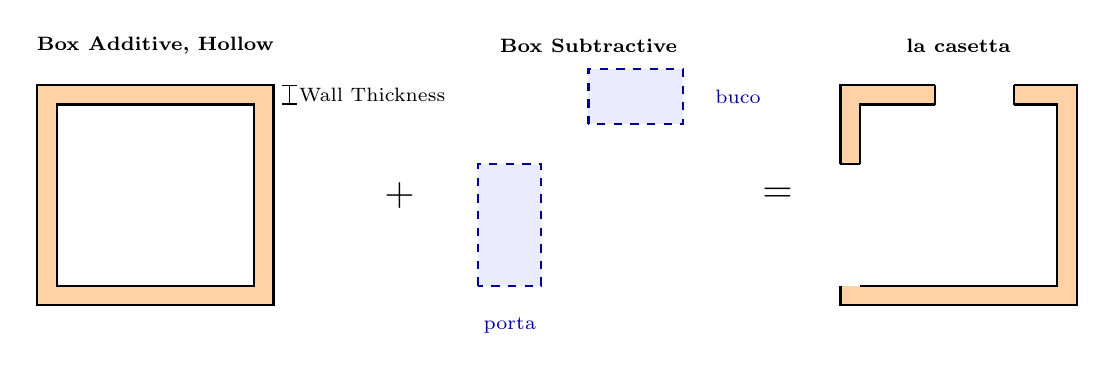
\begin{tikzpicture}[font=\footnotesize, x=1cm, y=1cm]
  % box additiva hollow (sezione)
  \node[font=\scriptsize\bfseries] at (1.5,3.3) {Box Additive, Hollow};
  \fill[orange!35] (0,0) rectangle (3,2.8);
  \fill[white] (0.25,0.25) rectangle (2.75,2.55);
  \draw[thick] (0,0) rectangle (3,2.8); \draw[thick] (0.25,0.25) rectangle (2.75,2.55);
  \draw[|-|, thin] (3.2,2.55) -- node[right, font=\scriptsize]{Wall Thickness} (3.2,2.8);
  \node at (4.6,1.4) {\Large $+$};
  % sottrattive
  \node[font=\scriptsize\bfseries] at (7.0,3.3) {Box Subtractive};
  \draw[thick, dashed, blue!60!black, fill=blue!8] (5.6,0.25) rectangle (6.4,1.8);
  \node[font=\scriptsize, blue!60!black] at (6.0,-0.25) {porta};
  \draw[thick, dashed, blue!60!black, fill=blue!8] (7.0,2.3) rectangle (8.2,3.0);
  \node[font=\scriptsize, blue!60!black] at (8.9,2.65) {buco};
  \node at (9.4,1.4) {\Large $=$};
  % risultato
  \begin{scope}[xshift=10.2cm]
    \node[font=\scriptsize\bfseries] at (1.5,3.3) {la casetta};
    \fill[orange!35] (0,0) rectangle (3,2.8);
    \fill[white] (0.25,0.25) rectangle (2.75,2.55);
    \fill[white] (-0.05,0.25) rectangle (0.3,1.8);
    \fill[white] (1.2,2.5) rectangle (2.2,2.85);
    \draw[thick] (0,1.8) -- (0,2.8) -- (1.2,2.8); \draw[thick] (2.2,2.8) -- (3,2.8) -- (3,0) -- (0,0) -- (0,0.25);
    \draw[thick] (0.25,1.8) -- (0.25,2.55) -- (1.2,2.55); \draw[thick] (2.2,2.55) -- (2.75,2.55) -- (2.75,0.25) -- (0.25,0.25);
    \draw[thick] (0,1.8) -- (0.25,1.8); \draw[thick] (1.2,2.55) -- (1.2,2.8); \draw[thick] (2.2,2.55) -- (2.2,2.8);
  \end{scope}
\end{tikzpicture}
\caption{Additive e Subtractive in sezione: una box additiva vuota (Hollow, con il suo
Wall Thickness) e due box sottrattive che la ``bucano'', una per la porta e una per il
buco sul soffitto da cui cadere nella stanza sottostante, come nella casetta costruita a
lezione. Ricostruzione schematica; le proporzioni sono indicative.}
\label{ue13:fig:csg}
\end{figure}

\paragraph{Il però: le brush sono pesanti.} ``Ora c'è un però, e il però è che le brush
sono \textbf{pesanti}.'' Se si riempie una scena di brush, ``perché volete diverse casette e
diverse zone dentro cui entrare'', ``si carica tanto sulla memoria del progetto''. Il
rimedio: \textbf{farla diventare una static mesh}. Nei Details della brush c'è il comando
per creare una static mesh dalla geometria (\emph{Create Static Mesh}, nella parte avanzata
dei Brush Settings), che chiede dove salvarla. Il docente lo fa con la casetta: nel
Content Browser compare ``un bloccone'', ma solo della brush selezionata (``se avessimo
selezionato tutte quante le brush, avremmo avuto un effetto diverso'': la mesh le avrebbe
comprese tutte). Il docente elimina la brush originale, ``non ci serve più'': la static mesh
che resta ``è molto meno pesante. Io posso riempirci la scena di questa roba qua.''
Bisognerebbe solo sistemarne il \textbf{pivot}, ``perché ce l'ho salvato col pivot
strano''. Un consiglio di ordine: invece di ``buttarla qui in mezzo al Content'', come ha
fatto lui, create ``una \emph{new folder} che chiamate, che ne so, \textbf{Blockout
Assets}'', e lì dentro mettete tutto quello che create. (Poi le elimina: a lui non servono.)

\paragraph{Approfondimento: perché le brush pesano, e Create Static Mesh.} Le geometry
brush sono la versione moderna della geometria \textbf{BSP} (\emph{binary space
partitioning}) delle vecchie versioni di Unreal: le brush additive e sottrattive vengono
combinate, nell'ordine in cui sono state create, in un'unica geometria del livello, che
l'editor ricalcola (\emph{Build Geometry}) quando le si modifica. Questa geometria non si
può istanziare, non ha LOD, ha UV e lightmap generate automaticamente e la sua collisione
è meno efficiente di quella di una mesh: per questo, oltre che per la memoria, Epic
raccomanda di usarle per il block out e di convertirle (o sostituirle) con static mesh
nel livello finale. Il comando \textbf{Create Static Mesh} salva la geometria delle brush
selezionate come asset \emph{Static Mesh}, con i materiali delle facce come slot; la
mesh nasce con il pivot all'origine del mondo o della prima brush, che si corregge con il
\emph{Modeling Mode} (strumento \emph{Pivot}) o riposizionandola. Nel libro di Romero e
Sewell le brush non compaiono: il libro costruisce i livelli con static mesh duplicate
(capitolo 9, il pavimento duplicato con Alt e trascinamento per raddoppiare l'area di
gioco). Quanto al modeling tool, il \emph{Modeling Mode} esisteva già come plugin
sperimentale nelle ultime versioni di Unreal~4, ma è con Unreal~5 che è diventato uno
strumento standard dell'editor: la frase del docente è vera nella sostanza. Funzionamento
generale dell'engine, salvo il riferimento al libro.

% ---------------------------------------------------------------------
\section{Le altre forme e il Brush Editing}
\label{ue13:sec:forme}

``Vediamo effettivamente cosa ci permettono di fare le altre brush.'' (La box sottrattiva il
docente se la tiene, ``almeno vediamo''.)

\paragraph{Cone.} Ha sempre le stesse impostazioni per le facce. Nei Brush Settings: un
valore \textbf{Z}, l'altezza; un \textbf{Outer Radius}; un \textbf{Inner Radius}, che non
si può modificare finché il cono non è \textbf{Hollow}: ``se io la rendo vuota'' si vede
com'è dentro, e si crea una struttura ``sulla base di quello che a me serve''. Il docente ci
mette dentro la box sottrattiva: ``una capannola mezza favola, una tenda''. Si può aumentare
il numero di lati (\textbf{Sides}): da 3, ``una piramide, anzi un D4'', fino a 500. A 500
``ha un po' stutterato, e non ci sarà mai un momento in cui ti servirà avere un cono così
preciso'', ma più facce lo rendono ``un po' più smussato''.

\paragraph{Cylinder.} ``Più o meno le stesse cose'': l'altezza, l'Outer Radius (``quanto è
largo effettivamente''), le facce come per il cono, Hollow o no, e il tipo, additivo o
sottrattivo.

\paragraph{Sphere.} Il \textbf{Radius}, ``quanto è ampia'', e la \textbf{Tessellation},
``quanti blocchi ha, quindi quanto è sferica''.

\paragraph{Linear Stair.} Tutto si basa sullo scalino, ``come anche le altre scale'': la
lunghezza del singolo scalino (\textbf{Step Length}), l'altezza (\textbf{Step Height}), la
larghezza (\textbf{Step Width}) e il numero di scalini (\textbf{Num Steps}): ``aumentando
gli scalini, aumenta l'altezza e aumenta la distanza''. Poi \textbf{Add to First Step},
``quanto in alto in più deve essere il primo scalino'': ``vedete, lui alza un tot''.

\paragraph{Curved Stair.} Altezza e larghezza dello scalino, e in più:
\begin{itemize}
  \item l'\textbf{Inner Radius}, il raggio del cerchio interno: ``se è molto largo, le
        scale vengono più arcuate'';
  \item l'\textbf{Angle of Curve}, ``quanto deve curvare la scala'': di default 90 gradi,
        ``però potreste fare anche 180, 270, anche 360 gradi'', se volete ``una singola
        chiocciola'';
  \item Num Steps e Add to First Step, ``esattamente allo stesso modo'';
  \item \textbf{Counter Clockwise}, per le scale ``che vanno nell'altra direzione''.
\end{itemize}
``Con tutte queste, poi potete andare a creare effettivamente delle static mesh.''

\paragraph{Spiral Stair.} ``Gli stessi parametri'': Inner Radius, Step Width, Step Height,
e in più lo spessore del singolo gradino (\textbf{Step Thickness}), ``perché è costruita
proprio a gradoni, ognuno di questi è un oggetto a sé stante, tutti attaccati l'uno con
l'altro''. C'è poi il numero di scalini \emph{per 360 gradi} (\textbf{Num Steps Per 360}):
``se voi dite che devono esserci 33 scalini per fare 360 gradi, poi dovete aggiungere
abbastanza scalini per arrivare a fare 360 gradi''; abbassandolo, con lo stesso numero
totale di scalini (``50, 60'') ne servono meno per fare un giro. Infine si può rendere
liscio il soffitto (\textbf{Sloped Ceiling}) o il pavimento (\textbf{Sloped Floor}), ``e
quindi avere una sorta di scivolo, una rampa'', e Counter Clockwise.

\paragraph{Il Brush Editing.} ``Prima facciamo un'ultima roba'': passare dalla
\textbf{Selection Mode} al \textbf{Brush Editing} (dal menu delle modalità dell'editor). Qui
si fanno ``piccole operazioni di modellazione'': selezionare un \textbf{vertice} e
spostarlo, una \textbf{faccia} e muoverla, un \textbf{edge} e muoverlo, ``in questo modo ci
andiamo a creare esattamente il tipo d'oggetto che serve a noi, anche se la forma che
serve a noi non c'era'' fra le brush. E lo \textbf{Split}: ``fa passare una serie di
vertici e di edge a tagliare'', una sezione dell'oggetto; ``si formano nuove facce, e
queste nuove facce possono essere prese e modificate''. ``Non so quanto spesso vi tornerà
utile fare un ecomostro del genere, però avete la possibilità di farlo.'' Un'avvertenza
emersa dalla prova: dopo le modifiche, l'oggetto ``è ancora una brush'', ma ``appena
l'andiamo a modificare'' dai Brush Settings ``ritorna come era precedentemente'': i
parametri ricostruiscono la forma da zero e cancellano le modifiche manuali.

\begin{table}[htbp]
\centering
\small
\begin{tabular}{@{}p{2.5cm}p{11.5cm}@{}}
\toprule
\textbf{Brush} & \textbf{Parametri (Brush Settings)} \\
\midrule
tutte & Brush Type: Additive / Subtractive; i materiali e le UV si impostano per faccia \\
Box & X, Y, Z; Wall Thickness (default 10); Hollow; Tessellated (solo se non hollow) \\
Cone & Z (altezza); Cap Z; Outer Radius; Inner Radius (solo se hollow); Sides (da 3 a
500); Align to Side; Hollow \\
Cylinder & Z; Outer Radius; Inner Radius (solo se hollow); Sides; Align to Side; Hollow \\
Sphere & Radius; Tessellation \\
Linear Stair & Step Length; Step Height; Step Width; Num Steps; Add to First Step \\
Curved Stair & Inner Radius; Step Height; Step Width; Angle of Curve (default
90$^\circ$); Num Steps; Add to First Step; Counter Clockwise \\
Spiral Stair & Inner Radius; Step Width; Step Height; Step Thickness; Num Steps Per 360;
Num Steps; Sloped Ceiling; Sloped Floor; Counter Clockwise \\
\bottomrule
\end{tabular}
\caption{Le geometry brush e i loro parametri. I nomi sono quelli dei Details di Unreal
Engine~5; quelli non letti a lezione (Cap Z, Align to Side) sono completati come
approfondimento.}
\label{ue13:tab:brush}
\end{table}

``Sono le cinque e mezza.'' Il docente annuncia che, al ritorno dalla pausa, si potrebbe
fare ``un piccolo block out utilizzando gli oggetti che avete'': le brush, le static mesh e
gli oggetti fatti con Igor, ``per cui magari vi piazzate dei collectible da raggiungere in
giro'', ``anche molto semplice''. Pausa di un quarto d'ora: ``facciamo 45''.

% ---------------------------------------------------------------------
\section{La pausa e la scelta del formato}
\label{ue13:sec:pausa}

(Durante la pausa la trascrizione contiene solo il blocco di testo ripetuto citato
nell'introduzione.) Alla ripresa c'è un problema di volume (``stavo leggendo il messaggio
che aveva scritto Augusto in chat'') e l'appello: Federico c'è, Guido ``c'è, ma non gli
funziona la telecamera'' (``basta che siete responsivi'').

\paragraph{La domanda del docente.} ``Ci stavo pensando adesso che stavamo fermi'': come
preferiscono strutturare le lezioni?
\begin{enumerate}
  \item una prima parte di spiegazione e una seconda in cui gli studenti ``provano a
        costruire qualcosa'', magari in streaming, ``così gli altri vedono anche cosa
        fate'' e il docente può commentare;
  \item tutte e tre le ore di spiegazione, con il lavoro pratico fra una lezione e l'altra
        e i feedback all'inizio della lezione successiva. Il tempo a disposizione cambia:
        ``da oggi, che è giovedì, fino a martedì avrete più tempo; da martedì a giovedì ne
        avrete meno''.
\end{enumerate}
Un primo studente preferisce la prima opzione, ``perché almeno abbiamo dei feedback diretti
e ci si può soffermare di più sulle varie cose''. Un altro la seconda, ``perché forse
riusciamo a fare più cose'', ``vediamo un po' più di argomenti''. Il docente avverte che le
cose che si faranno con lui ``sono tendenzialmente non troppo complesse, è più una
questione di metterle assieme'', e che non vorrebbe la situazione in cui ``io vi dico
facciamo questa cosa, la prossima volta me lo fate vedere e nessuno fa niente''. Edoardo,
alle prese con il caldo, dice che fare le cose fra una lezione e l'altra ``non è un peso''
se trova una soluzione; un altro: ``personalmente mi piace la seconda''. Il voto (``siete
dispari, quindi uscirà fuori una verità o l'altra''; ``per chi ci guarda da casa sarà tutto
in mano alle persone che erano qui'') premia la \textbf{seconda}: ``Tommaso, indipendentemente
dal tuo input, il popolo ha deciso di riempire la lezione con delle cose che magari faccio
io''.

Conseguenze: la lezione sullo \textbf{speed level design} andrà ``rimaneggiata'', ``perché
non so quanto ha senso che io mi metta a fare uno speed level per tre ore con voi che mi
guardate''; era ``una roba che mi sarebbe piaciuto far fare a voi''. Per la volta successiva,
a chi vuole, il docente chiede ``un piccolo livellino'' con geometrie e static mesh, ``per
giocare un po''': ``è molto bello sapere come funziona Unreal, però deve esserci del
\textbf{divertimento} nella creazione. Io mi devo divertire mentre creo il gioco.'' Le
indicazioni precise arrivano a fine lezione (sezione~\ref{ue13:sec:compiti}).

\paragraph{Che cosa fare nell'ora rimasta.} Personalizzare i parametri del bot in una gym
``è relativamente fine a se stesso'', ``un discorso abbastanza semplice'' che gli studenti
possono fare da soli. Meglio un altro actor interessante: le \textbf{luci}, e ``se riesco,
un accennino di post process''. Le luci si vedranno ``in un vuoto'', ``senza un dressing già
finito'', e si riprenderanno quando si parlerà di \emph{enrichment}, di dressing e di
ambienti, con lo speed level; per quella lezione il docente potrebbe preparare
``un ambientino'' o passare un pacchetto, ``così chi vuole lo fa assieme a me''. Le slide
non servono: ``faremo a braccio''. (Di nuovo problemi con Zoom: ``ogni volta che parto con la
stream non funziona il tasto destro''.) Il docente costruisce con una grande box un
ambientino chiuso (``così abbiamo un po' d'ombra''), invitando Filippo, che preferiva fare
le cose insieme, a sperimentare in parallelo. (Una parte della costruzione, nella
trascrizione, è incomprensibile: ``me la metà? E questa la facciamo? Giusto per fare
razzola''.)

% ---------------------------------------------------------------------
\section{Le luci: i tipi e la mobility}
\label{ue13:sec:mobility}

``Cos'è che non sta più funzionando in quella zona lì?'' Dentro la box: ``la luce del sole'',
risponde uno studente. La luce del sole è un tipo di luce, ``la signora
\textbf{Directional Light}''. Le luci di Unreal sono cinque: \textbf{Directional},
\textbf{Point}, \textbf{Spot}, \textbf{Rect} e \textbf{Sky Light}. Secondo la classificazione
del docente:
\begin{itemize}
  \item directional e sky light sono \textbf{luci ambientali};
  \item point e spot light si usano ``principalmente per l'illuminazione'';
  \item la rect light ``principalmente per i riflessi o per delle luci specifiche''.
\end{itemize}

\paragraph{Il costo dei rimbalzi.} ``Una cosa importante da dire è che il modo in cui Unreal
calcola le luci è simulando delle onde'' e il modo in cui ``queste onde luminose rimbalzano
sulle superfici''. Ci saranno situazioni in cui a una luce verranno chiesti ``troppi
rimbalzi, che equivalgono a troppi calcoli, che equivalgono a un peso molto elevato'':
bisogna stare attenti a come si posizionano le luci. (Sull'idea delle ``onde'' si veda
l'approfondimento alla fine della sezione.)

\paragraph{La Mobility.} ``Un parametro fondamentale che c'è in tutte le luci'' è la
\textbf{Mobility}: di default le luci sono \textbf{Stationary}, ma ci sono anche
\textbf{Static} e \textbf{Movable}. ``Non mi aspetto una risposta super completa, voglio
vedere se riusciamo ad arrivarci'' (``basta che ci passate sopra col mouse e ve lo dice
cosa fanno, però state con me''). Le ipotesi degli studenti: movable ``sarà tipo la luce di
una macchina''; stazionaria ``che sta ferma e non si muove'', ma statica ``mi sembra simile
come significato''; un altro propone ``statica un lampione, stazionaria il faro di una
macchina ferma, che potenzialmente si può muovere''; un altro ancora che la movable
``dovrebbe avere delle proprietà fisiche, magari condizionata dalla gravità'' (``la gravità
non c'entra''); un altro l'angolazione (``no, l'angolazione dipende dal tipo di luce che
utilizziamo''). Il docente rinuncia alla prova pratica (``qui c'è un po' di fregatura,
perché siamo in preview'') e parte dagli usi:
\begin{itemize}
  \item una luce \textbf{movable} è quella di ``una torcia a mano'', di una torcia
        elettrica che si punta, dei fari di una macchina, delle luci di un aereo: ``qualcosa
        in movimento'';
  \item una luce \textbf{stazionaria} è quella di un lampione, di un soffitto, ``di una
        qualsiasi luce di una casa'' \emph{dentro} il livello;
  \item una luce \textbf{statica} serve agli stessi scopi della stazionaria, ``ma fuori dal
        vostro livello''.
\end{itemize}
``Cosa cambia fra statica e stazionaria?'' Uno studente: ``nella stazionaria ci può
interagire un actor come il character''. ``Esatto.'' Le proprietà sono due: se si muove la
luce, l'ambiente reagisce?; se si passa davanti alla luce, la luce reagisce?
(figura~\ref{ue13:fig:mobility}):
\begin{itemize}
  \item la luce \textbf{statica} ``viene cucinata sulla scena'': è \emph{baked}
        completamente nell'editor e non si può modificare in gioco. Quando si
        \emph{buildano} le luci o si esporta il livello, ``la luce viene bakeata ed è
        impressa sulla scena''. Se si sposta l'actor della luce, la luce ``rimane dove è
        stata bakeata''; se il character ci passa davanti, la luce non reagisce. Si usa ``in
        tutti quei posti in cui so che non avrà interazioni e sarà soltanto luce
        d'atmosfera, luce d'ambiente''. È ``il tipo di luce più leggero'';
  \item la luce \textbf{stazionaria} ``se la muovo si rompe, ma se sta ferma e io ci passo
        davanti interagisce con me'': il character proietta ombre corrette, ma se si sposta
        la luce dopo il bake, la luce non si aggiorna;
  \item la luce \textbf{movable} ``fa entrambe le cose'': è completamente dinamica, reagisce
        agli oggetti e può essere spostata ``senza nessun problema''.
\end{itemize}

\begin{figure}[htbp]
\centering
\begin{tikzpicture}[font=\footnotesize, x=1cm, y=1cm,
  ue13col/.style={draw, thick, rounded corners=3pt, minimum width=4.0cm, minimum height=0.8cm,
                  align=center}]
  \node[ue13col, fill=gray!15] (st) at (0,0) {\textbf{Static}};
  \node[ue13col, fill=yellow!30] (sy) at (4.6,0) {\textbf{Stationary} (default)};
  \node[ue13col, fill=orange!30] (mv) at (9.2,0) {\textbf{Movable}};
  \node[align=left, anchor=north, text width=4.0cm] at (0,-0.6)
    {\textbf{bake}: sì, tutta\\ \textbf{si sposta in gioco}: no\\ \textbf{ombre dei personaggi}: no\\
     \textbf{costo}: il più basso\\[2pt] \emph{luce d'ambiente fuori dall'area di gioco}};
  \node[align=left, anchor=north, text width=4.0cm] at (4.6,-0.6)
    {\textbf{bake}: sì, la parte fissa\\ \textbf{si sposta in gioco}: no\\ \textbf{ombre dei personaggi}: sì\\
     \textbf{costo}: medio\\[2pt] \emph{lampioni, luci di casa, soffitti}};
  \node[align=left, anchor=north, text width=4.0cm] at (9.2,-0.6)
    {\textbf{bake}: no\\ \textbf{si sposta in gioco}: sì\\ \textbf{ombre dei personaggi}: sì\\
     \textbf{costo}: il più alto\\[2pt] \emph{torce, fari, luci di un aereo}};
  \draw[-{Stealth[length=2.5mm]}, very thick, gray] (-2.0,-3.3) -- node[below, font=\scriptsize]{più dinamica, più pesante} (11.2,-3.3);
\end{tikzpicture}
\caption{Le tre Mobility delle luci come le descrive il docente: che cosa viene
precalcolato (\emph{baked}), se la luce si può spostare in gioco, se reagisce ai personaggi
che le passano davanti, quanto pesa e per che cosa si usa.}
\label{ue13:fig:mobility}
\end{figure}

\paragraph{Approfondimento: onde, raggi e Lumen.} L'immagine delle ``onde'' è una
semplificazione del docente: Unreal non simula la luce come un'onda (niente interferenza o
diffrazione), ma come energia che viaggia in linea retta e rimbalza, cioè per
\emph{raggi}. Il calcolo dei rimbalzi (l'illuminazione \emph{globale}) avviene in due modi:
precalcolato, con \textbf{Lightmass}, che scrive il risultato nelle \emph{lightmap} delle
superfici al momento del build (luci static e stationary); o in tempo reale, con
\textbf{Lumen}, il sistema di illuminazione globale dinamica che Unreal Engine~5 attiva di
default nei progetti nuovi. Il principio del docente resta valido: più superfici e più
luci si sovrappongono, più calcoli servono, che siano fatti una volta nel build o a ogni
frame. Sulla stationary, un dettaglio in più: in gioco se ne possono cambiare colore e
intensità (non la posizione), e le ombre che proietta sugli oggetti fermi sono precalcolate,
mentre quelle degli oggetti in movimento sono dinamiche. Romero e Sewell (capitolo 4)
mettono la \emph{Mobility} di una point light a \textbf{Movable} proprio ``per poter
cambiare le proprietà della luce durante l'esecuzione'', quando la accendono e la spengono
da Blueprint. Funzionamento generale dell'engine, salvo il riferimento al libro.

% ---------------------------------------------------------------------
\section{La directional light e la sky light}
\label{ue13:sec:directional}

Il docente porta la directional light e la sky light ``tutte nello stesso posto''.
``Spostare queste luci non ha nessun tipo d'effetto.'' Perché?

\paragraph{La Directional Light.} Si può muoverla e scalarla ``come voglio e non cambia
assolutamente nulla. Ma se la ruoto, la luce reagisce.'' (``In questo caso reagisce anche''
un altro actor del cielo, ``perché è collegato'': la trascrizione dice ``la Schakespeare'' e
``la Schiapunsky'', con ogni probabilità la \emph{Sky Sphere} o la \emph{Sky Atmosphere}
del livello; il nome esatto non è ricostruibile.) La ragione: ``la directional light è
composta in una maniera abbastanza peculiare: è un \textbf{fascio di rette parallele} che
prende tutta la scena''. Spostarla non cambia nulla; ruotarla cambia ``il modo in cui viene
indirizzata la luminosità''. I parametri interessanti:
\begin{itemize}
  \item l'\textbf{Intensity}: aumentandola, ``va in questo caso a bruciare un pochino tutta la
        scena'' (``l'intensità della luce calcolata in X'': l'unità di misura nella
        trascrizione è incomprensibile; per la directional è il \emph{lux});
  \item il \textbf{Light Color}: una ruota dei colori per il colore della luce, la sua
        saturazione, ``quanto sarà scura, magari quanto sarà livida''. Se si vuole che più
        luci abbiano lo stesso colore, si copia il codice \textbf{Hex Linear} e lo si incolla
        nelle altre, ``il modo più comodo piuttosto che cercare a mano di replicare la stessa
        luce'': per esempio un corridoio in cui tutte le torce sono ``molto calde, molto
        accese, molto infuocate'';
  \item la \textbf{Temperature} (con \emph{Use Temperature}), per una luce ``tendenzialmente
        più calda o più fredda''; ``così, se volete fare \emph{Breaking Bad} quando sono in
        Messico, tutto giallo'';
  \item \textbf{Affects World}: ``questa luce che sto utilizzando ha effetto sul mondo? È una
        luce attiva o disabilitata?''. Serve, per esempio, a vedere ``come contribuisce alla
        scena'' una luce alla volta;
  \item \textbf{Cast Shadows}: la luce illumina comunque, ma proietta le ombre solo se è
        attivo;
  \item la \textbf{Dynamic Shadow Distance}: secondo il docente, ``quanto precisamente
        viene calcolata l'ombra, quanto è netta''. ``Non può essere notato adesso perché
        stiamo utilizzando solo geometrie''; con asset veri un valore basso si nota. Il
        docente cerca nel progetto una mappa già arredata per mostrarlo (``mi sa che non ne
        abbiamo, a parte quelle che ha fatto Igor'') e rimanda: ``la prossima volta mi
        preparo una scenetta carina a livello estetico''. È un parametro che ``tende ad
        appesantire un pochino le scene'', ma ``l'effetto che fa è talmente meglio rispetto a
        non averlo'': ``giocatevi un po' di potenza in più''.
\end{itemize}

\paragraph{Una sola per scena.} ``Non dovete mai avere \textbf{due directional} nella stessa
scena'': l'engine prova a calcolarle entrambe, ``fa molta fatica'' e ``il risultato è
tremendo'', con problemi di ombre calcolate in direzioni diverse. Allo stesso modo
``evitate di avere due sky sphere'', anzi, si corregge, due \textbf{sky light}: ``skylight e
directional light, una soltanto per scena''.

\paragraph{La Sky Light.} ``Funziona in maniera un po' diversa'', ``un po' più complessa'', e
``al momento non ci serve troppo indagarla''. Che cosa fa: ``è la luce che dà il
\textbf{mood}, la diffusione'', ``va a colorare l'aria, va a dare colore alla scena''. Si vede
cambiando il colore della sky light: cambiano di colore le \emph{ombre}. Per una scena al
tramonto, ``piuttosto che avere solo la directional che è arancione'', si media fra
directional e sky light, ``più tutta una serie di altre cose, perché utilizzeremo anche il
post process'' (la volta successiva). Fra i parametri, oltre all'intensità, quelli
dell'\textbf{ambient occlusion}: la distanza massima (\emph{Occlusion Max Distance}), il
contrasto (\emph{Contrast}) e ``quanto è moltiplicata'' (\emph{Occlusion Exponent} e
\emph{Min Occlusion}); e anche qui Cast Shadows e Affects World. ``Principalmente, mood
della scena e ambient occlusion.''

\paragraph{Approfondimento: Dynamic Shadow Distance, e due directional.} Il nome completo
del parametro è \emph{Dynamic Shadow Distance Movable Light} (o \emph{Stationary Light}, a
seconda della mobility): è la distanza dalla camera entro cui la directional disegna le
ombre dinamiche, divise in \emph{cascate} (\emph{Cascaded Shadow Maps}) di risoluzione
decrescente. Non è quindi la ``nettezza'' in sé, ma lo spazio su cui la risoluzione delle
ombre viene distribuita: oltre quella distanza le ombre dinamiche spariscono (restano solo
quelle precalcolate), e allungarla, a parità di cascate, rende le ombre vicine meno
dettagliate. In Unreal Engine~5, con le \emph{Virtual Shadow Maps} attive di default, questo
compromesso pesa molto meno. Sulle due directional, la regola del docente è la pratica
comune; a rigore Unreal ne supporta due solo come sole e luna dell'atmosfera (indice
\emph{Atmosphere Sun Light Index} 0 e 1), un caso particolare. Funzionamento generale
dell'engine.

% ---------------------------------------------------------------------
\section{Point light e spot light}
\label{ue13:sec:point}

``Passando a delle luci con cui andrete a smanettare molto ma molto di più'': le luci
``antropiche'', quelle che si useranno ``per fare quasi tutto'', \textbf{point light} e
\textbf{spot light}. ``Fra le due, qual è più leggera, più facile da calcolare,
indipendentemente dalla mobility?''

\paragraph{La domanda.} Uno studente risponde la point light, ``perché non si va a calcolare
anche la direzione''. ``È esattamente il contrario.'' La point light è a 360 gradi: ``lui
calcola contemporaneamente tutte le direzioni''. La \textbf{spot light} è più leggera
``perché non va a calcolare i rimbalzi della luce nelle altre direzioni'': ``la discriminante
è quella della direzione''. In una scena affollata, la spot illumina solo dove la si punta,
mentre la point ``va posizionata con attenzione perché va a colpire anche gli oggetti che ha
alle spalle'', ``indiscriminatamente dalla direzione''.

\paragraph{L'Attenuation Radius.} Per la point light, ``i due parametri più importanti sono
l'intensità e l'\textbf{Attenuation Radius}'', la sfera che si vede attorno alla luce.
``Indipendentemente dal fatto che io ho messo 10.000 miliardi di intensità, se il raggio non
tocca nulla la luce non illumina'' (o meglio, illumina solo dentro la sfera, ``quindi non
rimbalza su niente''). È ``il raggio massimo entro cui la luce avrà effetto'', e gestisce
un'attenuazione dalla sorgente fino al bordo: il \emph{gradiente} della luce. Con
un'intensità altissima, per un'attenuazione sensata bisogna ingrandire molto il raggio. Ma
anche con un'intensità bassa l'attenuazione arriva fino al bordo, e questo è il punto: il
raggio è ``il parametro che va gestito con attenzione'', ``perché determina con quanti
oggetti la luce andrà a compenetrare'', e quindi quante ombre dovrà proiettare. ``Anche se
l'intensità è molto bassa, nel momento in cui questo muro è all'interno del raggio,
l'engine dovrà calcolare'' l'ombra e la luce su quella superficie.

\paragraph{La X rossa.} ``Una cosa che vi capiterà sicuramente'': una luce con una
\textbf{X rossa} sopra. Il docente la riproduce mettendo più luci vicine (al primo tentativo
``non abbastanza'': i raggi erano piccoli). Vuol dire che ``l'engine ha rinunciato a far
proiettare ombre a questa luce'': la luce illumina comunque, ``ma non proietta ombre perché
ci sono troppe altre luci con cui questa luce sta compenetrando''. L'engine lo segnala come
problema, ``non grave''. I rimedi sono due: dire noi alla luce di non proiettare ombre
(Cast Shadows disattivato), così l'engine ``non cercherà costantemente di proiettarle'';
oppure \textbf{ridurre il raggio} ``a tal punto da non farlo compenetrare con troppe cose''.
``Non riempite la vostra scena di luci, piuttosto utilizzate \textbf{poche luci molto
significative}.''

\paragraph{Il corridoio.} L'esempio: un corridoio con una fila di luci. Mentre il
personaggio passa, le ombre sono corrette ``fino a che non arriviamo qui vicino'': lì la
luce viene calcolata ``come se questa non ci fosse'', e l'ombra viene proiettata dalle due
luci ai lati. ``Vedete, qui skippa, qui salta'': l'ombra della luce con la X non c'è, c'è
solo quella della luce ``un po' più lontana'', mentre altrove l'ombra è ``molto più forte,
molto più precisa, molto più netta''. ``Se replicate questo esperimento per conto vostro, vi
rendete conto che è abbastanza semplice da replicare.''

\paragraph{La sorgente: Source Radius, Soft Source Radius, Source Length.} Come illuminare
un corridoio ``piuttosto che avere una luce per torcia, una luce per punto''? Si modifica la
\textbf{sorgente}: ingrandendo il \textbf{Source Radius} e allungando la \textbf{Source
Length}, la luce non parte più da un punto ma ``da un cilindro, da una capsula'', ed è
``più distribuita''. Il raggio può anche essere zero, ``se volete una linea e basta''. È
così che si fanno illuminazioni particolari, ``tipo un locale illuminato unicamente dalla
luce dei \textbf{neon}'': mesh con materiali \textbf{emissive}, ``che quindi già emettono una
piccola luce di loro'', più luci distribuite ``in maniera più omogenea'' in questo modo. Il
\textbf{Soft Source Radius} ``serve per creare un'altra lucina interna, come quando puntate
una torcia verso il muro'': una parte più attenuata all'esterno e una meno attenuata
all'interno (``si vede meglio con la spot''; il docente non riesce a mostrarlo bene). Più
sotto ci sono di nuovo Affects World e Cast Shadows, e lo \emph{scattering} con la nebbia
volumetrica (\emph{Volumetric Scattering Intensity}), che servirà quando si userà una
nebbia (la trascrizione dice ``una FOD'', con ogni probabilità \emph{fog}); poi ``molti, molti
parametri'' per le ombre (risoluzione, comportamento sulle pendenze). ``Non tutti vi
servono'', ``a meno che non vogliate fare proprio il \emph{light artist}''. (``Non l'ho
detto prima'': anche la point light ha il Light Color, ``per fare le vostre luci da inferno,
da nightclub, da \emph{Night City}''.)

\paragraph{La spot light.} È fatta a \textbf{cono}, quindi si ruota. Intensità e Light
Color come le altre; l'\textbf{Attenuation Radius}, qui, ``non dipende da quanto è la
sfera, ma è la lunghezza del cono'', ``quanto in là viene proiettata'': ``se sta così non
colpisce il muro, così illumina questa parte del muro''. Poi due angoli
(figura~\ref{ue13:fig:luci}):
\begin{itemize}
  \item l'\textbf{Outer Cone Angle}, che gestisce il cono;
  \item l'\textbf{Inner Cone Angle}, il cono interno, ``l'effetto torcia'': nella parte
        colpita dall'inner cone ``ci sarà una minore attenuazione''. Con i due angoli vicini
        il bordo è netto; ``volendo potete avere anche un cono che non attenua mai alla
        base, che attenua soltanto sulla distanza''. Questo cono serve a determinare la
        \emph{sfumatura}, ``ed è anche quello che faceva l'altro nella point, ma con questo
        si nota meglio''.
\end{itemize}
Anche qui Source Radius, Source Length e Soft Source Radius, e i parametri delle ombre.

\paragraph{La domanda sull'effetto accecante.} Uno studente chiede se, guardando
direttamente la luce, ci sia ``l'effetto accecante''. ``No, assolutamente no.'' L'effetto
``tipo quando guardi il sole'' si crea con il \textbf{post process}, che il docente vuole
far vedere ``quando abbiamo una mappa che non sia soltanto delle geometrie'' (con un
pacchetto di mesh e mappe già fatte: ``sono abbastanza sicuro che questo pacchetto dovesse
avere delle mappe''). Con i parametri del post process si aggiungono \textbf{bloom} e
\textbf{lens flare}. Altro esempio: i \textbf{god rays} (``god shaft''), ``una luce molto
forte che entra dalla finestra e c'è questa proiezione luminosa che taglia la scena''.
``Quella roba lì con la luce non puoi farla. Ti serve la luce, ma devi andare a manipolare
il modo in cui la telecamera vede la luce con la post produzione.'' Per questo ``la post
produzione va fatta dopo le luci'': ``prende l'illuminazione della scena e ci aggiunge delle
lenti, degli effetti''. Fra le ``lenti'', oltre al bloom: la messa a fuoco, la distorsione,
la \emph{chromatic aberration}.

\begin{figure}[htbp]
\centering
\begin{tikzpicture}[font=\footnotesize, x=1cm, y=1cm]
  % point light
  \node[font=\scriptsize\bfseries] at (1.6,3.4) {Point Light};
  \shade[inner color=yellow!70, outer color=white] (1.6,1.6) circle (1.5);
  \draw[dashed, thick, orange!70!black] (1.6,1.6) circle (1.5);
  \fill[orange] (1.6,1.6) circle (0.08);
  \draw[-{Stealth[length=1.6mm]}] (1.6,1.6) -- (2.66,2.66);
  \node[font=\scriptsize, align=center] at (1.6,-0.5) {Attenuation Radius = sfera;\\360$^\circ$: colpisce anche\\ciò che ha alle spalle};
  % spot light
  \begin{scope}[xshift=4.4cm]
    \node[font=\scriptsize\bfseries] at (1.6,3.4) {Spot Light};
    \fill[yellow!25] (0.2,2.8) -- (3.2,0.2) -- (0.9,0.0) -- cycle;
    \fill[yellow!65] (0.2,2.8) -- (2.55,0.4) -- (1.55,0.1) -- cycle;
    \draw[dashed, thick, orange!70!black] (0.2,2.8) -- (3.2,0.2);
    \draw[dashed, thick, orange!70!black] (0.2,2.8) -- (0.9,0.0);
    \fill[orange] (0.2,2.8) circle (0.08);
    \node[font=\scriptsize, anchor=west] at (2.7,1.3) {Outer Cone};
    \node[font=\scriptsize, anchor=west, fill=white, inner sep=1pt] at (1.25,1.15) {Inner};
    \node[font=\scriptsize, align=center] at (1.6,-0.5) {Attenuation Radius =\\lunghezza del cono};
  \end{scope}
  % rect light
  \begin{scope}[xshift=8.8cm]
    \node[font=\scriptsize\bfseries] at (1.8,3.4) {Rect Light};
    \fill[yellow!30] (0.9,2.4) -- (2.7,2.4) -- (3.4,0.2) -- (0.2,0.2) -- cycle;
    \draw[very thick, fill=orange!60] (0.9,2.4) rectangle (2.7,2.6);
    \draw[very thick, gray!70!black] (0.9,2.4) -- (0.55,1.95);
    \draw[very thick, gray!70!black] (2.7,2.4) -- (3.05,1.95);
    \node[font=\scriptsize, anchor=east] at (0.55,2.0) {Barn Door};
    \node[font=\scriptsize, align=center] at (1.8,-0.5) {Source Width $\times$ Height;\\Barn Door Angle e Length};
  \end{scope}
\end{tikzpicture}
\caption{Le tre luci locali e i parametri che ne determinano la forma: la sfera di
attenuazione della point light, i due coni della spot light (nel cono interno
l'attenuazione è minore) e la sorgente rettangolare della rect light, con le ``porte da
stalla'' che ne restringono il fascio. Schema indicativo, non in scala.}
\label{ue13:fig:luci}
\end{figure}

\paragraph{Approfondimento: la X rossa, il costo delle ombre e i god rays.} La X rossa ha
una causa precisa: è il limite delle luci \textbf{stationary} sovrapposte. Le ombre
precalcolate delle stationary vengono scritte in quattro canali di una texture, quindi in
un punto qualsiasi del livello possono sovrapporsi al massimo \textbf{quattro} luci
stationary con le ombre attive (la directional conta come una); la quinta, segnata con la X
rossa, ripiega sulle ombre interamente dinamiche, più costose, o le perde (l'editor la
elenca nel \emph{Map Check}). Per questo i rimedi del docente funzionano: ridurre
l'Attenuation Radius toglie la sovrapposizione; disattivare Cast Shadows toglie la luce dal
conteggio; un'altra via è rendere la luce static o movable. Sul costo: la ragione per cui
una spot light è più economica di una point light sta soprattutto nelle ombre, perché una
spot proietta le ombre con una sola \emph{shadow map} orientata, mentre una point light ne
ha bisogno in tutte le direzioni (una \emph{cube map} di sei facce). Sui \textbf{god rays},
la frase del docente va presa nel suo senso: in Unreal l'effetto si ottiene con le opzioni
\emph{Light Shaft Occlusion} e \emph{Light Shaft Bloom} della directional light, o con la
\emph{Exponential Height Fog} con la nebbia volumetrica attiva; i light shaft sono
comunque un effetto calcolato sull'immagine della camera, quindi della stessa natura del
post process, come dice il docente. L'abbagliamento guardando il sole viene dal
\textbf{bloom} e dall'\textbf{esposizione automatica} (\emph{Eye Adaptation}), entrambi
impostati in un \textbf{Post Process Volume}. Romero e Sewell (capitolo 9) ricordano che il
\emph{Post Process Volume} e il \emph{Lightmass Importance Volume} del livello ``vanno
scalati per coprire l'area di gioco'' quando la si allarga, ``perché servono per
l'illuminazione e gli effetti''; e nel capitolo 12 che la qualità del post processing
(``motion blur e bloom'') e delle ombre (``i dettagli delle ombre hanno spesso un impatto
drammatico sulle prestazioni'') è fra le impostazioni di \emph{Engine Scalability}.
Funzionamento generale dell'engine, salvo i riferimenti al libro.

% ---------------------------------------------------------------------
\section{La rect light}
\label{ue13:sec:rect}

``Ora mi sono scordato le rect light.'' ``Sono un po' strane'': sembrano ``una spotlight,
ma tipo rettangolare'', e invece sono diverse. Si usano principalmente per le
\textbf{illuminazioni industriali}, ``le classiche luci quadrate da fabbrica'', o ``molto
più spesso'' per i \textbf{riflessi}: ``il riflesso della televisione su un pavimento''.
Vanno usate ``soltanto su oggetti rettangolari'' che proiettano una luce specifica, ``come
un'insegna al neon, di quelle dei locali''. ``Se devo farmi calcolare dei riflessi, lo
faccio utilizzando la rect light perché dà dei risultati più precisi.''

I parametri ``non sono troppo diversi'': intensità, colore, Attenuation Radius ``che ormai
abbiamo imparato a conoscere'', la larghezza e l'altezza della sorgente (\emph{Source Width},
\emph{Source Height}). Ciò che cambia:
\begin{itemize}
  \item il \textbf{Barn Door Angle}: la sorgente è un rettangolo centrale ``più una
        struttura lungo il rettangolo'', che Unreal chiama \emph{barn door} (``come si
        traduce?'', chiede il docente; ``la stalla'', risponde uno studente: le alette dei
        proiettori da set, dette appunto \emph{porte da stalla}). Cambiando l'angolo è
        ``come se ci fosse un'ostruzione'': le alette si piegano e la luce va solo in avanti;
        al massimo, la luce arriva fino a terra; nel mezzo, un effetto sfumato;
  \item la \textbf{Barn Door Length}, ``quanto è grande questa lente'', per ``un effetto tipo
        i riflettori degli stadi'', che illuminano ``una parte specifica, molto tagliata,
        molto netta'';
  \item la \textbf{Source Texture}: ``la texture che noi andiamo a inserire diventa il tipo di
        luce che viene messo'', come un'insegna o un televisore che proietta una luce
        particolare; ``è come se andasse a proiettare la luce attraverso un filtro, per
        spiegarlo in modo brutto''. Il docente cerca una texture riconoscibile nel progetto
        (``queste non vanno bene'') senza trovarla, e l'esempio resta a parole;
  \item anche qui la Temperature e Affects World.
\end{itemize}

% ---------------------------------------------------------------------
\section{Il build delle luci e i riflessi}
\label{ue13:sec:build}

``Stavo per scordare una delle parti fondamentali.'' La differenza fra static, stationary e
movable si vedeva ``molto meglio sulla quarta edizione''; ma anche sulla quinta ``dovete
stare attenti'': ``vi capiterà di fare dei livelli in cui avete un'illuminazione, poi andate
a buildare e la luce che vi ritrovate alla fine non è la luce che pensavate di avere''.
Questo perché le luci \textbf{statiche e stazionarie} hanno bisogno di essere
\textbf{buildate}.

\paragraph{La qualità del build.} Quando si fa il build bisogna scegliere la qualità con cui
calcolare le luci (\emph{Lighting Quality}): di default è \textbf{Preview}, ``la qualità
più veloce'', in cui ``vengono calcolati meno rimbalzi''; quando si pubblica un gioco si usa
\textbf{Production}, il livello più alto, che viene calcolato al build e ``rimane bakeato
sul livello''. Se non si fa il build, le luci statiche e stazionarie ``rimangono delle
preview''.

\paragraph{La ``bestemmia''.} ``Oppure utilizzate questa cosa che sto per dire, sarà una
bestemmia: utilizzate \textbf{solo luci movable}.'' Le movable sono pesanti, ``quindi non
utilizzate solo luci movable, chiaramente''; ma per un livello \emph{molto piccolo}, ``in cui
avete 2--3 luci massimo'', e che serve in fretta, avere luci movable ``che sono esattamente
come le vedete alla fine'' può tornare comodo. ``Se dovete illuminare un livello con 20 e
passa luci, non mettete solo luci movable'': mettete luci static e stationary e fate il
build.

\paragraph{Il menu Build.} Si possono buildare diverse cose, ``pezzo per pezzo'': le luci,
le \textbf{reflection capture} (``ecco che mi mancava, i riflessi''), la visibilità statica
(\emph{Precompute Static Visibility}), il \textbf{landscape} (``che poi vedremo la prossima
volta''), e così via; \textbf{Build All Levels} ribuilda tutto. ``Con la quinta edizione,
tutto sommato, ve la cavate'': in Unreal~4, senza il build, ci sarebbero scritte
\textbf{Preview} sparse per la scena e in alto \textbf{Lighting needs to be rebuilt}.
``Se mai vi capita di lavorare su una versione precedente di Unreal, sappiate che quella
scritta in alto è perché non avete buildato le luci''. In ogni caso: ``quando avete finito
il livello fate sempre un build generale''.

\paragraph{Le Reflection Capture.} I riflessi ``sono abbastanza scollegati
dall'illuminazione, ma funzionano in maniera simile'': anche loro sono \textbf{volumi} che
influenzano zone specifiche e vanno buildati. Si trovano fra i volumi: \textbf{Box
Reflection Capture}, \textbf{Planar Reflection} e \textbf{Sphere Reflection Capture}.
Prendendo la sfera, ``semplice da vedere'': ha un raggio di influenza (di default 3000), che
si ingrandisce e si riduce, e vi si possono assegnare mappe specifiche. Quando si fa il
build, ``catturano tutto quello che c'è all'interno della sfera e calcolano i riflessi sulle
superfici riflettenti''.

\paragraph{Quali superfici riflettono?} ``Perché anche se io buildo qui adesso lui non mi
farà vedere niente di diverso?'' Il docente rimanda alla lezione sui materiali: uno studente
ricorda i parametri ``quanto rifletto la luce, l'opacità''. ``Esatto'': i parametri che
contano sono \textbf{Metallic}, \textbf{Specular} e \textbf{Roughness}, ``soprattutto
Specular e Roughness'', che determinano quanto il materiale sarà riflettente. I materiali
della scena di prova non lo sono; con una roughness ``particolarmente bassa'' e una specular
``particolarmente alta'', tutti gli oggetti nell'area di cattura verrebbero riflessi sulle
superfici capaci di rifletterli: ``le pozzanghere, i pavimenti lucidi, gli specchi''. ``Magari
ci ritorniamo nel momento in cui abbiamo un ambiente più costruito, che non sia solo
blocchi.''

\paragraph{Approfondimento: il build in Unreal Engine 5.} Il motivo per cui ``con la quinta
ve la cavate'' è \textbf{Lumen}: nei progetti nuovi di Unreal Engine~5 l'illuminazione
globale e i riflessi sono calcolati in tempo reale, e una scena illuminata da luci movable
(o da stationary e static non ancora buildate) appare già come apparirà in gioco; i livelli
dei template, inoltre, partono spesso senza illuminazione precalcolata. Il build con
Lightmass serve quando si sceglie l'illuminazione precalcolata, di solito per ragioni di
prestazioni (piattaforme mobili, VR, scene molto statiche), e in quel caso valgono tutte le
avvertenze del docente: il build a qualità Production prima di pubblicare, il
\emph{Lightmass Importance Volume} attorno all'area di gioco, e il controllo del messaggio
``Lighting needs to be rebuilt'' (in Unreal~5 segnalato in modo meno vistoso). Anche le
\emph{Reflection Capture} perdono importanza con i riflessi di Lumen, ma restano il
ripiego quando Lumen è disattivato. La Sphere Reflection Capture ha di default un
\emph{Influence Radius} di 3000 unità (30 metri), il valore letto a lezione. Funzionamento
generale dell'engine; il libro di Romero e Sewell non tratta il build delle luci.

% ---------------------------------------------------------------------
\section{I compiti per martedì e la chiusura}
\label{ue13:sec:compiti}

``Abbiamo una decina di minuti.'' Le luci, ``accennate al volissimo'', si rivedranno con il
post process e con lo speed level, ``se riesco a farvi vedere qualcosina, almeno di che
cos'è concettualmente''. Uno studente chiede delle \emph{linee guida} per il lavoro della
volta successiva: ``delle specie di linee guida''. ``Molto fumose, molto generiche, però così
per darvi qualcosina'':
\begin{enumerate}
  \item una \textbf{gym} in cui si sono calcolati i parametri del proprio personaggio ``che
        ritenete importanti per il gameplay''. La Max Sprint Distance da 26 m serve solo se
        nel gioco ci sono cose a tempo: ``se voi volete fare soltanto un platform, magari
        questa cosa non vi serve''. Pensate ``a seconda del tipo di block out che volete
        fare'' e misurate quanto in alto salta, quanto velocemente si muove, quanto lontano
        salta, le differenze fra lo sprint e il salto, magari con una gravità modificata;
        le misure vanno tenute ``da una parte, all'interno del livello in cui andrete a fare
        il block out'';
  \item \textbf{smanettare con i parametri del bot}, BP\_Bot2, ``in modo da avere un tipo di
        esperienza che magari funziona meglio per il vostro gioco''. Esempio in diretta: il
        \textbf{Walkable Floor Angle}, ``44'' di default. Il docente fa delle rampe di
        pendenze diverse: su alcune il bot sale, su una più ripida ``lo fa scivolare giù''.
        Così si possono fare ``delle parti in cui il vostro robot non può andare, che non
        sono semplicemente dei muri''. O una gravità ``meno lunare''; o una camminata più
        veloce: ``io trovo che la camminata di base del robot, per i miei gusti, sia un po'
        lenta, quindi magari l'andrei a modificare''. E, ``una cosa carina'', il
        \textbf{margine di manovra e di errore}: il bot ``salta e non si muove a mezz'aria,
        ha un pessimo controllo a mezz'aria''; con l'\textbf{Air Control} a 1 ``si muove come
        se non fosse in aria''. ``Quanta libertà di movimento voglio dare al mio giocatore? Per
        quale motivo?'' La gym serve anche a rispondere a domande come: ``so che il mio
        personaggio salta 4 metri in avanti e 2 in alto: posso fare questo salto? E se posso
        farlo, è comodo farlo?'';
  \item un \textbf{piccolo block out} in cui l'obiettivo è prendere da \textbf{tre a cinque
        collezionabili}, ``ognuno ottenuto in una maniera diversa'': esplorando,
        saltellando, usando gli oggetti delle lezioni precedenti, ``schivando i colpi della
        mitraglietta'', ``quello che volete''. Serve a familiarizzare ``con l'idea di fare delle
        piccole sfide che il giocatore deve superare per raggiungere degli obiettivi''.
\end{enumerate}
Alla lezione successiva il docente chiederà che cosa è stato modificato e perché: ``poi
magari ci facciamo una chiacchiera sul perché avete deciso di dare quel tipo di parametro
al robottino e cosa volevate farci, che è l'inizio del design: iniziare a pensare a questi
numeri, in che modo influenzano l'esperienza del giocatore''.

Per chi ha problemi di surriscaldamento: ``provateci'', ``stiamo lavorando principalmente con
dei blocchi'', ``non c'è nulla di pesante da un punto di vista grafico''; ``le cose pesanti
verranno più avanti, quando cominceremo a utilizzare elementi estetici''. ``Penso di essermi
mangiato le mie parole tipo infinite volte, però di averle dette talmente tante volte che
era chiaro il concetto.'' Nessuna domanda. ``Ci becchiamo martedì prossimo'': per qualsiasi
cosa, il \textbf{Discord}, anche per mostrare il proprio lavoro.

\paragraph{Approfondimento: il compito visto dai libri.} Il compito mette insieme i temi
della giornata nell'ordine in cui Totten li presenta: prima le metriche (la gym), poi il
whiteblocking (il block out), poi le sfide costruite sulle metriche e sulle abilità del
personaggio. Due criteri dal suo capitolo 2 sono utili come controllo: ogni sfida dovrebbe
usare una metrica misurata (un salto vicino al limite, una distanza vicina alla Max Sprint
Distance, una pendenza oltre il Walkable Floor Angle) e dovrebbe essere \emph{leggibile},
cioè comunicare al primo sguardo se e come si supera, come il blocco da 1,40 m della
lezione. Romero e Sewell (capitolo 13) mostrano come trovare e piazzare rapidamente
actor di supporto dal \emph{Place Actors Panel} (lo stesso pannello usato a lezione per le
brush), comodo per disseminare il livello di collezionabili e punti di riferimento.

% ---------------------------------------------------------------------
\begin{table}[htbp]
\centering
\small
\begin{tabular}{@{}p{4.6cm}p{3.2cm}p{6.2cm}@{}}
\toprule
\textbf{Misura o valore} & \textbf{Valore} & \textbf{Dove e a che serve} \\
\midrule
Max Sprint Distance & 26 m & la corsa con una barra di stamina; limite per inseguimenti e
distanze fra ricariche \\
Margine sullo sprint & circa 20 m & dove mettere una ricarica di stamina \\
Walk Jump / Sprint Jump & 4 m / 6 m & la lunghezza dei salti del bot con Jump Z Velocity
modificata \\
Limiti per i salti di un platform & circa 2,20--2,30 m in alto, 5,80 m in lungo & le sfide
del livello, sotto i massimi \\
Blocchi d'altezza & 1; 1,40; 1,60; 1,80; 2 m & il feeling del salto; 1 m superato
``male'', 1,40 m no \\
Max Step Height & 45 cm (provato con 40 cm e 1 m) & il gradino che si sale camminando \\
Walkable Floor Angle & ``44'' (44,77$^\circ$) & la pendenza oltre cui il bot scivola \\
Jump Z Velocity & 420 $\to$ 700 (poi 600--650) & l'altezza del salto: con 700 oltre i 2 m \\
Air Control & fino a 1 & il controllo in aria (1 = come a terra) \\
Porte nella slide della gym & 4$\times$4, 2$\times$4, 2$\times$3, 2$\times$2,5,
2$\times$2 m & l'esperienza di passarci, con la camera in terza persona \\
Max comfortable wall run & 12 m (discesa da 13--14 m) & la slide della gym \\
Griglia del pavimento & 1 m, quadratini da 20 cm & leggere le misure; snapping a 10 cm \\
Box di prova & 600; Wall Thickness 10 $\to$ 50 & la casetta con le brush \\
Sides del Cone & da 3 a 500 & la precisione del cono \\
Sphere Reflection Capture & raggio 3000 & la zona di cattura dei riflessi \\
\bottomrule
\end{tabular}
\caption{Le misure e i valori della giornata. I valori del salto e della corsa sono quelli
trovati in diretta dal docente, che li definisce ``molto non calcolati'': il compito è
trovare i propri.}
\label{ue13:tab:misure}
\end{table}

\begin{table}[htbp]
\centering
\small
\begin{tabular}{@{}p{5.4cm}p{8.6cm}@{}}
\toprule
\textbf{Sintomo} & \textbf{Causa e rimedio} \\
\midrule
Il bot supera il blocco da 1 m ``scivolando'' & la capsula sale sullo spigolo: ostacolo
poco leggibile; alzarlo (1,40 m è chiaramente insuperabile) o renderlo chiaramente
superabile \\
Il bot sale su un ostacolo da 40 cm senza saltare & è sotto la Max Step Height (45 cm):
abbassarla se non va bene \\
Max Step Height a 1 m non fa salire il bot & salvare e compilare; poi restano i limiti della
capsula e degli altri parametri (non risolto a lezione) \\
Cambiare la Jump Z Velocity non ha effetto & si sta modificando il Blueprint sbagliato: il
personaggio in gioco è BP\_Bot2 \\
Il materiale della brush si deforma & la brush è stata scalata: usare X, Y, Z dei Brush
Settings \\
Il materiale va su una faccia sola & le brush hanno un materiale per faccia: assegnarlo a
ogni faccia \\
Inner Radius non modificabile & il cono (o il cilindro) non è Hollow \\
Tessellated non ha effetto & la box è Hollow \\
Le modifiche del Brush Editing spariscono & si è cambiato un parametro dei Brush Settings,
che ricostruisce la forma \\
La scena con molte brush è pesante & Create Static Mesh, poi eliminare la brush; mettere le
mesh in una cartella Blockout Assets; sistemare il pivot \\
Spostare la directional non cambia nulla & è un fascio di rette parallele: va ruotata \\
Ombre sbagliate con due directional (o due sky light) & una sola per scena \\
Una luce illumina poco nonostante l'intensità & l'Attenuation Radius non raggiunge le
superfici \\
X rossa su una luce, niente ombre & troppe luci (stationary) sovrapposte: ridurre il raggio
o disattivare Cast Shadows \\
Nel corridoio l'ombra ``salta'' & la luce con la X non proietta ombre: come sopra; o una sola
luce allungata (Source Length) \\
La luce finale non è quella vista nell'editor & luci static e stationary non buildate:
Build, qualità Production \\
Scritte Preview e ``Lighting needs to be rebuilt'' (Unreal 4) & build delle luci mancante \\
Le Reflection Capture non mostrano nulla & i materiali non sono riflettenti: Roughness bassa,
Specular alta \\
Il tasto destro non funziona durante la condivisione & problema di Zoom, non risolto \\
\bottomrule
\end{tabular}
\caption{I problemi incontrati durante la lezione, con la causa e il rimedio.}
\label{ue13:tab:errori}
\end{table}

\begin{table}[htbp]
\centering
\footnotesize
\begin{tabular}{@{}p{5.8cm}p{8.2cm}@{}}
\toprule
\textbf{Strumento, actor o impostazione} & \textbf{Che cosa fa} \\
\midrule
Level design document & descrive il livello in modo chiaro, né generico né costrittivo \\
Layout (piantina) & la mappa 2D del livello, con legenda; si sbaglia senza costi \\
Gym (test level) & il livello in cui si misurano le metriche del personaggio \\
Block out & il livello rifatto con sole geometrie, per testare il gameplay \\
Landmark & oggetto riconoscibile che dà identità e orienta \\
Snapping della griglia & sposta gli actor a passi fissi (10 cm) \\
Text Render (approfondimento) & testo nel livello, per i cartelli delle misure \\
Character Movement & il componente dei parametri di movimento del personaggio \\
Quick Add (menu), voce Geometry & aggiunge le brush e gli altri actor \\
Place Actors Panel & pannello agganciabile con tutti gli actor da piazzare \\
Geometry Brush: Box, Cone, Cylinder, Sphere, Linear, Curved e Spiral Stair & le forme di
base per il block out \\
Brush Type: Additive / Subtractive & aggiunge geometria; la toglie (buchi, porte, finestre) \\
Hollow, Wall Thickness, Tessellated & vuota; spessore dei muri; divisa in triangoli \\
Create Static Mesh (Brush Settings) & salva la brush come static mesh, più leggera \\
Brush Editing (modalità) & sposta vertici, edge e facce; Split per tagliare \\
Directional Light & il sole: rette parallele, conta solo la rotazione \\
Sky Light & il colore dell'ambiente, il mood, l'ambient occlusion \\
Point Light / Spot Light / Rect Light & luce in tutte le direzioni; a cono; da una sorgente
rettangolare \\
Mobility: Static / Stationary / Movable & tutta precalcolata; fissa ma reattiva; dinamica \\
Intensity, Light Color, Hex Linear & l'intensità; il colore; il codice da copiare \\
Temperature (Use Temperature) & luce più calda o più fredda \\
Affects World / Cast Shadows & accende o spegne la luce; ne attiva le ombre \\
Dynamic Shadow Distance & la distanza entro cui la directional disegna ombre dinamiche \\
Attenuation Radius & il raggio (o la lunghezza del cono) entro cui la luce agisce \\
Source Radius / Soft Source Radius / Source Length & la dimensione della sorgente; la
sfumatura; la lunghezza (luce a capsula) \\
Inner / Outer Cone Angle & il cono interno meno attenuato; il cono esterno \\
Barn Door Angle / Length, Source Texture & le alette della rect light; la texture
proiettata \\
Volumetric Scattering Intensity & l'interazione della luce con la nebbia volumetrica \\
Build: Lighting Quality (Preview, Production) & la qualità del calcolo delle luci \\
Build All Levels, Build Reflection Captures & ricalcola tutto; solo i riflessi \\
Box / Sphere Reflection Capture, Planar Reflection & catturano l'ambiente per i riflessi \\
Metallic, Specular, Roughness (materiale) & quanto una superficie riflette \\
Post process: bloom, lens flare, messa a fuoco, distorsione, chromatic aberration &
effetti sull'immagine della camera (la prossima lezione) \\
\bottomrule
\end{tabular}
\caption{Gli strumenti, gli actor e le impostazioni della tredicesima lezione.}
\label{ue13:tab:nodi}
\end{table}

% ---------------------------------------------------------------------
\section*{Punti chiave del capitolo}
\addcontentsline{toc}{section}{Punti chiave del capitolo}

\begin{itemize}
  \item Le ultime quattro lezioni sono di \textbf{level design}: teoria di base, block out e
        geometry brush, Landscape e Foliage Mode, luci, post process, dressing e, alla fine,
        piccoli livelli da condividere come eseguibili sul Discord.
  \item Ci si ispira alla \textbf{realtà}, non alla \emph{fiction}: la mappa di un altro
        gioco è già filtrata dal suo game design. Il \textbf{level design} nasce dal
        \textbf{game design} e dal modo in cui si muove il personaggio.
  \item Il \textbf{level design document} è chiaro e leggibile, né troppo generico né
        troppo costrittivo. Prima del block out c'è il \textbf{layout}: una piantina con
        legenda (a quadretti per un platform) per prevedere l'esperienza e mettere il
        giocatore ``sui binari''.
  \item La \textbf{gym} è il livello in cui si misurano le metriche del personaggio
        (altezza e lunghezza dei salti, corsa, pendenze, porte, altezza da accovacciati);
        che cosa misurare dipende dal tipo di gioco. In terza persona le porte si fanno
        ``falsamente alte'' per non far sbattere la camera.
  \item Il \textbf{block out} ricostruisce il livello con sole geometrie per testare il
        gameplay prima dell'estetica: misure, durata, landmark, ricompense, guide come le
        bandiere, arene da allargare o stringere.
  \item In engine: pavimento a griglia e snapping per misurare; la \textbf{Max Sprint
        Distance} (26 m a lezione) decide inseguimenti, ricariche e distanze fra
        ostacoli, sempre con un margine d'errore.
  \item Il \textbf{feeling}: un ostacolo superato ``scivolando'' con la capsula è pessima
        comunicazione; uno chiaramente troppo alto è buona comunicazione.
  \item Il \textbf{Character Movement}: Gravity Scale, Mass, Max Step Height (45),
        Walkable Floor Angle, Max Walk Speed, \textbf{Jump Z Velocity} (420 di default,
        una velocità iniziale), \textbf{Air Control}, nuoto e volo. Si misurano i salti
        risultanti (4 m camminando, 6 m correndo a lezione) e si progettano le sfide un po'
        sotto i massimi.
  \item Le \textbf{geometry brush} servono a prototipare: materiali per faccia, dimensioni
        dai \textbf{Brush Settings} e non dalla scala, Hollow e Wall Thickness,
        \textbf{Additive} e \textbf{Subtractive} per bucare. Sono pesanti: \textbf{Create
        Static Mesh}, in una cartella \emph{Blockout Assets}. Il Brush Editing modifica
        vertici, edge e facce, ma i Brush Settings ricostruiscono la forma.
  \item Le luci: \textbf{Directional} e \textbf{Sky Light} (una per scena), \textbf{Point},
        \textbf{Spot} e \textbf{Rect}. La \textbf{Mobility}: Static (precalcolata, la più
        leggera), Stationary (fissa ma reagisce ai personaggi, il default), Movable
        (dinamica, la più pesante).
  \item L'\textbf{Attenuation Radius} decide con quante superfici la luce interagisce e
        quindi quanto costa; la \textbf{X rossa} segnala troppe luci sovrapposte senza
        ombre: ridurre il raggio o togliere Cast Shadows. Poche luci molto significative;
        la spot costa meno della point.
  \item Static e stationary vanno \textbf{buildate} (Production prima di pubblicare); solo
        movable va bene per livelli minuscoli. Le \textbf{Reflection Capture} vanno buildate
        e si vedono solo su materiali riflettenti (Roughness bassa, Specular alta). Bloom,
        lens flare e abbagliamento sono \textbf{post process}.
  \item Il compito: una gym con le metriche del proprio bot, parametri modificati e
        motivati, e un piccolo block out con \textbf{da tre a cinque collezionabili},
        ognuno raggiunto in modo diverso.
\end{itemize}

%
%  Tutte le etichette di questo capitolo hanno il prefisso "ue13:"
%  (ue13:cap:..., ue13:sec:..., ue13:fig:..., ue13:tab:...), e tutti gli
%  stili TikZ hanno il prefisso "ue13" (ue13box, ue13room, ...) per non
%  collidere con chiavi native di TikZ né con quelli delle lezioni
%  precedenti. Il capitolo è autonomo: non contiene \ref verso altri
%  capitoli (i rimandi alle lezioni precedenti sono a parole). Le figure
%  sono ricostruzioni schematiche di quanto mostrato e detto a lezione
%  (le slide e il video non sono nella trascrizione), non copie delle
%  schermate del docente. Dove la trascrizione è troppo rovinata per
%  ricostruire un dettaglio, il capitolo lo dice invece di inventarlo.
% =====================================================================

\chapter[Gym, block out e luci]{Introduzione al level design: la gym, il block out
e le luci}
\label{ue13:cap:leveldesign}

Questa è la \textbf{tredicesima lezione} del corso breve di \textbf{introduzione a Unreal
Engine}, e la prima con un \textbf{nuovo docente}. Le dodici lezioni precedenti, con
\textbf{Igor}, hanno costruito un piccolo repertorio di meccaniche (il personaggio
\textbf{bot} che cammina, corre e salta, la stamina, i collezionabili, la torretta che
spara, le porte che si aprono, le pedane che salgono e scendono, la luce che si accende,
i materiali fisici dell'acqua e della roccia). Le ultime \textbf{quattro lezioni} cambiano
prospettiva: non più ``come si programma una meccanica'', ma \textbf{come si costruisce un
livello} che quelle meccaniche le metta alla prova. ``L'idea delle mie lezioni, di queste
mie ultime quattro lezioni, sarà quella di spiegare un po' il \emph{workflow} che c'è alla
base della creazione di un livello e iniziare a mettere su dei livellini.''

Il docente non dice mai il proprio nome nella trascrizione. Le lezioni precedenti
annunciavano che il corso sarebbe proseguito ``con Davide'' e con il \emph{level design}, e
qui il docente parla di Igor come di un collega (``io e Igor proviamo le cose che avete
fatto''): il docente è quindi, con ogni probabilità, \textbf{Davide}, ma è una deduzione del
capitolo, non qualcosa che la lezione dica. Nel resto del capitolo è semplicemente ``il
docente''.

La giornata ha tre parti. La prima è un ``filo di teoria'', ``niente di troppo pesante'':
da dove si prende l'ispirazione per un livello, il \textbf{level design document}, il
\textbf{layout} (la piantina), la \textbf{gym} (il livello di prova in cui si misurano le
capacità del personaggio) e il \textbf{block out} (il livello rifatto con sole geometrie).
La seconda è pratica, in Unreal: si abbozza una gym con il bot, si misurano la corsa e i
salti, si toccano i parametri del \textbf{Character Movement} e si conoscono le
\textbf{geometry brush}, lo strumento classico per fare un block out. La terza, dopo la
pausa, è una panoramica sulle \textbf{luci}: i tipi di luce di Unreal, la loro
\emph{mobility}, i parametri principali, il costo delle ombre, il \emph{build} delle luci e
le \emph{reflection capture}. In chiusura, il compito per la lezione successiva: una gym
propria e un piccolo block out con da tre a cinque collezionabili.

Tre avvertenze di lettura, come per le lezioni precedenti. La prima: la trascrizione è
automatica e storpia moltissimi nomi. Unreal è ``Real'', ``un reale'' e ``Arial''; la
\textbf{gym} è ``GIM'' e ``JIM''; il \textbf{block out} è una volta ``plot out'' e il
\emph{blockouting} ``lockout''; \textbf{Kratos} è ``Gratos'' e ``Grados''; la
\textbf{Max Sprint Distance} è ``Mazda Sprint'' e ``Max Print Distance''; il Blueprint del
bot, \textbf{BP\_Bot2} (``character bot 2''), è una volta ``bottegger''; il
\textbf{Walkable Floor Angle} è ``workable floor angle'' e ``Walk and roll Flow Rainbow'';
la \textbf{static mesh} è ``state mesh'' e ``state Mesh''; il \textbf{Foliage Mode} è
``Folliage Mode''; il \textbf{Light Color} è ``let color'' e ``LED color''; il codice
\textbf{Hex Linear} è ``l'ex liner'' e ``gli ex''; \textbf{Affects World} è ``FXWord'';
l'\textbf{ambient occlusion} è ``ambiente occlusion''; il \textbf{Source Radius} è ``la
sorsa'' e il \textbf{Soft Source Radius} ``SRADUS soft SRADUS''; la \textbf{Source Length}
è ``la lent''; le \textbf{Barn Door} sono ``bar and door''; la \textbf{Planar Reflection}
è ``Lanar Reflection Capture''; \emph{baked} (``cotto'', precalcolato) è reso con
``becata'', ``abbicata'', ``baicata'' e ``vacato''; \emph{Breaking Bad} è ``break in
bed''. Dove la ricostruzione è sicura il capitolo usa la forma corretta; dove non lo è
riporta la forma della trascrizione e lo dice. La seconda: in alcuni punti il
riconoscimento vocale produce testo estraneo alla lezione. In apertura ci sono frasi su
``la situazione interna a livello politico'' e su ``gli egiziani'', poco dopo una frase
ripetuta (``io personalmente sono a favore di questa cosa''), a metà della parte sulle
scale una serie di frasi senza senso (``non preoccupatevi se non mi ricordo bene le mie
relazioni'') e, durante la pausa, un lungo blocco ripetuto decine di volte (``grazie a
tutti per l'attenzione che ci ha spiegato'', ``qual è la risposta che ci può essere?''):
non appartengono alla lezione e sono stati ignorati. La terza: le slide e il video
mostrati dal docente non sono nella trascrizione; il capitolo ricostruisce le immagini da
ciò che il docente dice mentre le indica, completa i nomi esatti dei parametri di Unreal
Engine~5, distingue le prove dalle conclusioni e dichiara i punti in cui la trascrizione
lascia un buco.

\paragraph{Come leggere questo capitolo.} Il capitolo segue l'ordine della lezione. Le
figure ricostruiscono la mappa di un metroidvania commentata dal docente, il percorso a
quadretti di un platform, la gym costruita in diretta, il ``feeling'' dei due salti
provati, le brush additive e sottrattive, le tre \emph{mobility} delle luci e le forme
delle luci locali. Le tabelle riassumono le misure della giornata, i parametri del
Character Movement, i parametri delle brush e delle luci, i problemi incontrati e le
impostazioni usate. Qua e là, dei paragrafi di \textbf{approfondimento} collegano la
lezione al libro di Marcos Romero e Brenden Sewell, \emph{Blueprints Visual Scripting for
Unreal Engine 5}, il testo di riferimento per questa parte del libro, al libro di
Christopher W.\ Totten, \emph{An Architectural Approach to Level Design}, che tratta
proprio i temi teorici della giornata, e a qualche nozione tecnica generale su Unreal
Engine~5; sono segnalati come tali e non fanno parte della lezione.

Il percorso del capitolo:
\begin{enumerate}
  \item l'\textbf{apertura} e il programma delle ultime quattro lezioni
        (sezione~\ref{ue13:sec:apertura});
  \item \textbf{da dove si parte}: la realtà o un altro gioco
        (sezione~\ref{ue13:sec:ispirazione});
  \item il \textbf{level design document} e il \textbf{layout}
        (sezione~\ref{ue13:sec:layout});
  \item la \textbf{gym}, il livello di prova (sezione~\ref{ue13:sec:gym});
  \item il \textbf{block out} e il caso di God of War (sezione~\ref{ue13:sec:blockout});
  \item in engine: la gym, la griglia e la \textbf{distanza di sprint}
        (sezione~\ref{ue13:sec:sprint});
  \item i \textbf{salti} e il \emph{feeling} del personaggio
        (sezione~\ref{ue13:sec:salti});
  \item i parametri del \textbf{Character Movement} (sezione~\ref{ue13:sec:cmc});
  \item le \textbf{geometry brush} (sezioni \ref{ue13:sec:brush} e~\ref{ue13:sec:forme});
  \item la \textbf{pausa} e la scelta del formato delle lezioni
        (sezione~\ref{ue13:sec:pausa});
  \item le \textbf{luci}: tipi e \emph{mobility} (sezione~\ref{ue13:sec:mobility}),
        directional e sky light (sezione~\ref{ue13:sec:directional}), point e spot light
        (sezione~\ref{ue13:sec:point}), rect light (sezione~\ref{ue13:sec:rect}), il
        \emph{build} e i riflessi (sezione~\ref{ue13:sec:build});
  \item i \textbf{compiti} per martedì e la chiusura (sezione~\ref{ue13:sec:compiti}).
\end{enumerate}

% ---------------------------------------------------------------------
\section{L'apertura e il programma delle ultime quattro lezioni}
\label{ue13:sec:apertura}

\paragraph{L'audio e il caldo.} I primi minuti sono di prova tecnica. Il docente ha
``cambiato la postazione del PC'' e chiede più volte se lo si sente bene, se è ``basso'', se
si sentono ``ventole in sottofondo'': ``se capita che mentre parlo mi si taglia la voce,
fatemelo sapere''. Il motivo: ``lo scorso anno, in questo periodo'', facendo lezione per lo
stesso corso, ``il computer fondeva lavorando su Unreal e streamando contemporaneamente'', e
ha dovuto comprare ``una di quelle pedanine'' con le ventole da mettere sotto il portatile,
``così almeno non cade la connessione o non crasha Unreal''. Il caldo è un tema anche per
gli studenti: uno di loro (Edoardo, a giudicare dal seguito) dice che ``il caldo non me lo
permette particolarmente'' e che sta cercando ``una soluzione per far funzionare il
computer''.

\paragraph{Chi c'è.} Il docente chiede quanti fossero, di solito, alle lezioni con Igor:
``più o meno sette''. Si aspetta qualche minuto, fino alle 16:10, ``se arrivano altre due o
tre persone''. Nel frattempo chiede se qualcuno abbia ``cominciato a smanettare'' per conto
proprio con Unreal, ``al di là di quello che stava spiegando Igor'': Edoardo no, oltre alle
lezioni; dagli altri nessuna risposta.

\paragraph{Il programma.} ``Magari riusciamo a fare qualcosina in più, magari facciamo
qualcosina in meno'', ma il piano delle quattro lezioni è questo:
\begin{itemize}
  \item ``un filo di teoria'', ``un'idea alla base'', ``in modo che quando andremo a creare
        dei livelli avremo almeno le idee un filo più chiare su cosa stiamo cercando di
        fare e come dovremmo costruire le cose'';
  \item i \textbf{block out} e quindi le \textbf{geometry brush} (l'argomento di oggi);
  \item ``se ci riesco'', più avanti, il \textbf{modeling mode} per le static mesh,
        ``questo magari verrà rimandato'';
  \item alcune delle modalità di Unreal, come il \textbf{Landscape Mode} e il
        \textbf{Foliage Mode}, e come possono tornare utili ``a seconda che stiamo creando
        dei livelli in interna o in esterna'';
  \item ``sicuramente la gestione delle luci, perlomeno una base di \emph{lighting}'', e
        con il lighting ``una base di post produzione'';
  \item ``un minimo di \textbf{dressing}'': si passerà dalle ``prime mappine fatte
        unicamente in geometrie'', quelle di oggi, a livelli ``esteticamente un pelo più
        curati''.
\end{itemize}
Il docente chiede se qualcuno sia iscritto al corso di design o di grafica 3D: la parte di
oggi copre ``principalmente quello che fa un \emph{designer} all'interno della creazione di
un livello''; la parte estetica ``spesso e volentieri viene rimandata ai grafici 3D, però è
importante comunque sapere qualcosina''.

\paragraph{L'esercitazione finale.} ``Cosa più importante'': il docente vorrebbe chiudere
con una vera \textbf{esercitazione} (``non so se farlo nell'ultima lezione o se darvelo per
il post''), in cui gli studenti creano qualcosa mentre lui dà dei feedback, e da cui escono
degli \textbf{eseguibili} da caricare sul Discord, ``in modo che a vicenda voi possiate
provare i livellini degli altri'', e che ``io e Igor'' proveranno lasciando dei feedback.
``Nulla di troppo impegnativo'': serve a ``iniziare a mettere mano un po' alla creazione di
livelli''. I livelli si costruiranno con le meccaniche programmate nelle lezioni
precedenti. (La trascrizione dice ``con i tool che io vi ho fatto, diciamo, fatto fare per
foto programmare le scorse lezioni'': il senso è, con ogni probabilità, \emph{i tool che
Igor vi ha fatto programmare}.)

% ---------------------------------------------------------------------
\section{Da dove si parte: la realtà o un altro gioco?}
\label{ue13:sec:ispirazione}

``Sono le quattro e dieci, sono passate in realtà'', e si comincia, con le slide. ``Da dove
partiamo quando vogliamo andare a creare un livello?'' Il grande dubbio è se partire
``dall'osservazione della realtà'' o da ``una mappa, da un videogioco che è stato già
creato da qualcun altro''. L'esempio: si vuole fare una mappa \emph{open} di
\textbf{Manhattan}, ``come stiamo vedendo qui con \emph{Spider-Man}''. A che cosa ci si
ispira per la struttura della mappa?

\paragraph{Le risposte degli studenti.} Il primo studente risponde: alla realtà, ``perché
mi sembra più fedele'', ``è una base che abbiamo sempre, ce l'abbiamo lì pronta'', ``è una
riproduzione più originale''. Il docente approva: la realtà è originale, non c'è bisogno di
``andare a cercare altri titoli che hanno fatto qualcosa ispirato a quello a cui noi ci
siamo ispirati''; esistono anzi ``tutta una serie di tool e di siti'' che permettono di
prendere le \textbf{height map} di una città specifica e di ricrearla dentro un engine. Poi
chiede se qualcuno voglia difendere l'altra opzione. Un secondo studente: trasformare la
realtà in poligoni ``richiede tempo'', mentre prendendo la mappa di un altro videogioco
``si può risparmiare un po' di tempo''. ``Ah, beh, sì, se possiamo rubare gli asset da un
altro videogioco cambia tanto'', scherza il docente, ma ``è una cosa che lascia un po' il
tempo che trova'': gli asset che servivano a quel gioco ``non sono proprio gli asset che
servono a noi''.

\paragraph{La risposta: la realtà, perché non è filtrata.} ``La risposta chiara e diretta è
quella per cui siete andati all'inizio'': ci si ispira alla \textbf{realtà}, perché è
\textbf{originale} e \textbf{non filtrata}. Non filtrata vuol dire che \emph{Spider-Man},
per costruire la sua Manhattan, ha dovuto ``estrapolare dalla realtà cose che si
incastravano particolarmente bene con il \emph{game design} previsto dal gioco''. La
componente principale di quel gioco è il \emph{traversal} con le ragnatele, il muoversi
fra i palazzi ad alta velocità; per una mappa soddisfacente da quel punto di vista
servono ``tanti palazzi alti'', e quindi si rimuove ``una grossa parte di Manhattan che non
ci interessa'' perché non si adatta al gameplay. Se nel nostro gioco non si oscilla fra i
palazzi, ``la mappa che \emph{Spider-Man} seleziona è scarsamente rilevante'': conviene
tornare all'originale. Magari nel nostro gioco ``facciamo delle rapine'' e serve ``una
parte della mappa molto più piccola'', in cui entrare negli edifici.

``Ci ispiriamo alla realtà e non alla \emph{fiction}, perché la fiction non è
necessariamente quello di cui abbiamo bisogno. Il game design di un altro gioco sarà
diverso dal nostro.'' E da qui il principio che regge tutta la giornata: il \textbf{level
design} ``dovrà essere largamente ispirato da quello che è il nostro game design'', dall'idea
di gameplay, ``dal modo in cui vogliamo, per esempio, far muovere il personaggio''.

\paragraph{Assassin's Creed e l'acqua.} Secondo esempio, \emph{Assassin's Creed}
ambientato a Roma. Il docente esita sul capitolo (``se non ricordo male \emph{Assassin's
Creed 2}, no, forse è \emph{Brotherhood}. È \emph{Brotherhood}''): è effettivamente
\emph{Brotherhood} il capitolo ambientato a Roma. Il ricordo del docente è che gli
sviluppatori avessero voluto inserire un'isola sul fiume (la trascrizione dice ``l'isola di
Berlina'': con ogni probabilità l'\textbf{Isola Tiberina}) per sfruttare un'innovazione,
il percorso nell'acqua, così da raggiungere ``i punti che sono molto coperti dalle
guardie''. Il docente stesso si corregge a metà (``ah, no, c'era l'acqua nel 2, vabbè, non
ricordo''): i dettagli storici sono incerti, ma il punto è chiaro. ``Diamo la possibilità
al giocatore di sfruttare le nuove meccaniche di gameplay per avere situazioni diverse,
situazioni nuove.''

\paragraph{E le nostre meccaniche?} Il docente ha visto le cose fatte con Igor: ``i
collezionabili, la torretta che spara, le porte che si aprono, le pedane che si alzano e si
abbassano''. ``In che modo il level design può andare a far leva su quelle componenti
lì?'' I collezionabili possono essere gli \textbf{obiettivi}; attorno a loro ci sono
\textbf{ostacoli} da capire come superare: ``passare davanti a una torretta senza farci
ammazzare'', ``capire come aprire la giusta sequenza di porte per arrivare a prendere il
collezionabile'', ``fare il giusto parkour fra le pedane in movimento''. È, in piccolo,
il compito che chiude la lezione.

\paragraph{Approfondimento: progettare sulle capacità del personaggio.} Totten
(\emph{An Architectural Approach to Level Design}, capitolo 2) dice la stessa cosa con
l'esempio di \emph{Metal Gear Solid}: ``progettare sul gameplay non significa solo
misure'', ma anche progettare sulle abilità specifiche del personaggio, come i modi di
movimento; i livelli di un gioco \emph{stealth} sono costruiti attorno alla possibilità di
nascondersi dietro i muri e sbirciare dietro gli angoli. È la versione positiva del
discorso di Spider-Man: non si copia la mappa di un altro gioco perché quella mappa era
costruita sulle abilità di un altro personaggio.

% ---------------------------------------------------------------------
\section{Il level design document e il layout}
\label{ue13:sec:layout}

``Una volta che abbiamo capito effettivamente cosa vogliamo dal nostro gioco'', si scrive un
\textbf{level design document}. ``Non parlerò troppo dei documenti perché non è questa la
sede''; la cosa importante è che siano \textbf{leggibili da tutti}, \textbf{chiari}, e che
dicano \textbf{come è strutturato il livello}. Il documento ha due vincoli opposti:
\begin{itemize}
  \item \textbf{non troppo generico}: il docente immagina di scrivere la mappa che ha in
        testa e di passarla a Edoardo, ``l'incaricato di fare il block out'': Edoardo
        ``deve essere in grado di capire precisamente tutto quello che io voglio da questa
        mappa dal documento che ho scritto'';
  \item \textbf{non troppo costrittivo} (la trascrizione dice ``costruttivo''): non deve
        ``limitare troppo Edoardo, che comunque ci deve mettere un po' del suo''.
\end{itemize}

\paragraph{Il layout: la piantina.} Una parte fondamentale della creazione di un livello,
e del documento, è il \textbf{layout}: ``fare una mappa, una piantina''. Perché? ``Perché
ci permette di sbagliare senza grossi problemi.'' Improvvisare direttamente nell'engine va
bene per una mappa molto semplice; per una mappa complessa ``ci troveremmo spesso a dire:
ah no, questa cosa non va bene'', e a rifare. ``In questa sede non avremo il tempo né
l'obiettivo'' di fare layout accurati, e si partirà direttamente dai block out; ma è
importante sapere che \textbf{prima del block out c'è la piantina}.

\paragraph{La piantina numerata.} La prima slide mostra (``qui in basso a sinistra'') una
pianta con dei numeri e una \textbf{legenda}. Il docente la legge come esempio:
\begin{enumerate}
  \item il punto in cui il giocatore \emph{spawna};
  \item il punto in cui trova la prima arma;
  \item il punto in cui trova dei nemici;
  \item il punto in cui ``si passa da piano a piano'', cioè da livello a livello.
\end{enumerate}
Ne esce un percorso: ``io parto da qui'', attraverso una zona in cui ``magari non c'è
niente, è una roba più \emph{straightforward} che mi permette di familiarizzare con
l'ambiente''; poi ``scendo giù'' nella zona dei nemici, ``ma non ho armi'': devo passare
``senza farmi notare'', prendere l'arma, tornare indietro ed eliminare i nemici.

\paragraph{Il platform a quadretti.} Lo stesso vale per i giochi in 2D, dove le misure
contano ancora di più. Se il personaggio salta ``tre quadratini in altezza e tre
quadratini in orizzontale'', la mappa va disegnata a quadretti ``per sapere in anticipo
come potrò far saltare il mio personaggio''. L'esempio della slide, alla \emph{Super
Mario}: all'inizio si fanno prendere ``i primi blocchetti'', i primi potenziamenti, e si fa
saltare il primo ostacolo, ``un salto molto semplice''; poi una scaletta, per far capire
che si può salire; poi un salto più complesso, su una piattaforma più piccola da cui
scendere; e così via, finché si arriva a salti ``al massimo dell'altezza e della
lunghezza'', che devono essere ``molto precisi'', e ad altri tipi di ostacoli
(figura~\ref{ue13:fig:platform}). ``Serve per avere le idee chiare'' e ``poter calcolare
bene'' il percorso.

\begin{figure}[htbp]
\centering
\begin{tikzpicture}[font=\footnotesize, x=0.42cm, y=0.42cm,
  ue13blk/.style={draw, fill=brown!35},
  ue13pow/.style={draw, fill=yellow!60},
  ue13jmp/.style={-{Stealth[length=1.8mm]}, thick, blue!60!black, dashed}]
  % griglia
  \draw[gray!30, step=1] (0,0) grid (32,9);
  % terreno
  \fill[brown!55] (0,0) rectangle (14,1);
  \fill[brown!55] (18,0) rectangle (24,1);
  \fill[brown!55] (29,0) rectangle (32,1);
  % blocchi potenziamento
  \draw[ue13pow] (3,4) rectangle (4,5); \draw[ue13pow] (4,4) rectangle (5,5);
  \node[font=\scriptsize] at (4,5.6) {potenziamenti};
  % primo ostacolo
  \draw[ue13blk] (7,1) rectangle (8,2);
  % scaletta
  \draw[ue13blk] (10,1) rectangle (11,2); \draw[ue13blk] (11,1) rectangle (12,3);
  \draw[ue13blk] (12,1) rectangle (14,4);
  % piattaforma piccola
  \draw[ue13blk] (15.5,5) rectangle (16.5,5.6);
  % piattaforma lontana, salto al limite
  \draw[ue13blk] (20,1) rectangle (22,2);
  \draw[ue13blk] (25.5,5) rectangle (26.5,5.6);
  % percorso
  \draw[ue13jmp] (6.3,1.2) .. controls (7,3.6) .. (8.6,2.2);
  \draw[ue13jmp] (13.6,4.2) .. controls (15,6.8) .. (15.9,5.8);
  \draw[ue13jmp] (16.4,5.8) .. controls (17.5,6.5) .. (18.6,1.2);
  \draw[ue13jmp] (22,2.2) .. controls (24.5,8.6) .. (25.9,5.8);
  \draw[ue13jmp] (26.4,5.8) .. controls (28,7) .. (29.4,1.2);
  % etichette
  \node[font=\scriptsize, align=center] at (7.5,-1.1) {1. salto\\semplice};
  \node[font=\scriptsize, align=center] at (12,-1.1) {2. scaletta};
  \node[font=\scriptsize, align=center] at (16.5,-1.1) {3. piattaforma\\piccola};
  \node[font=\scriptsize, align=center] at (25,-1.1) {4. salto al massimo\\di altezza e lunghezza};
  % misure
  \draw[red!70!black, thick, |-|] (-0.6,1) -- node[left, font=\scriptsize]{3} (-0.6,4);
  \draw[red!70!black, thick, |-|] (0,9.5) -- node[above, font=\scriptsize]{3 quadretti} (3,9.5);
\end{tikzpicture}
\caption{Il layout di un platform 2D disegnato a quadretti, come nell'esempio della slide:
conoscendo il salto del personaggio (qui tre quadretti in altezza e tre in lunghezza, i
valori citati a voce dal docente), si dispongono ostacoli via via più difficili, fino ai
salti al limite. Ricostruzione schematica: la slide non è nella trascrizione e le
posizioni sono indicative.}
\label{ue13:fig:platform}
\end{figure}

\paragraph{La mappa di un metroidvania.} L'ultima slide del layout è ``una roba del
genere'': da immaginare ``come la mappa di un metroidvania''. Il docente la percorre ad alta
voce, ed è un piccolo trattato di progettazione dei percorsi (figura~\ref{ue13:fig:metroid}):
\begin{itemize}
  \item si parte in alto e si scende fino a una \textbf{stanza rossa}, ``un'area
        esplorabile solo con dei power up'';
  \item si continua a scendere: certe direzioni sono chiuse, e c'è uno
        \textbf{shortcut} ``che però va aperto nell'altra direzione'', quindi si può solo
        andare giù;
  \item in fondo si prende il \textbf{power up}, ``magari un doppio salto, o un salto a
        parete'', con cui si può risalire: ``adesso mi si aprono diverse strade'';
  \item da lì si può esplorare, raccogliere un oggetto (``ci sarà sicuramente un
        oggetto''), salire nell'\textbf{area segreta}, o andare al \textbf{checkpoint},
        la \emph{safe room};
  \item più giù ci sono dei \textbf{nemici}: battuti quelli, si apre lo shortcut ``in modo
        che poi posso avanzare, se muoio, senza dover ribattere i nemici'';
  \item si prende una \textbf{chiave}, che serve per arrivare al \textbf{boss}; battuto
        il boss, si apre lo shortcut e si scende di piano. ``Se dovessi morire al piano di
        sotto, dal checkpoint potrei semplicemente scendere giù, superare lo shortcut che
        adesso ho già aperto e scendere dalle scale.''
\end{itemize}
``Fondamentalmente, ci facciamo delle mappe per cercare di prevedere e di strutturare quale
sarà l'esperienza del giocatore'', ``cercare di capire come posso costringere il giocatore
sui binari che a me interessano''.

\begin{figure}[htbp]
\centering
\begin{tikzpicture}[font=\scriptsize, x=1cm, y=1cm,
  ue13room/.style={draw, thick, fill=gray!10, minimum width=1.7cm, minimum height=0.8cm,
                   align=center},
  ue13path/.style={-{Stealth[length=2mm]}, thick},
  ue13short/.style={-{Stealth[length=2mm]}, thick, dashed, green!50!black}]
  \node[ue13room, fill=blue!12] (start) at (3.4,0) {inizio};
  \node[ue13room, fill=red!25] (red) at (6.8,0) {stanza rossa\\(serve power up)};
  \node[ue13room] (c1) at (3.4,-1.6) {corridoio};
  \node[ue13room] (c2) at (3.4,-3.2) {pozzo};
  \node[ue13room, fill=yellow!40] (pu) at (3.4,-4.8) {power up\\(doppio salto)};
  \node[ue13room, fill=purple!15] (sec) at (0,-1.6) {area segreta};
  \node[ue13room] (obj) at (0,-3.2) {oggetto};
  \node[ue13room, fill=green!15] (safe) at (6.8,-3.2) {checkpoint\\(safe room)};
  \node[ue13room, fill=orange!25] (en) at (6.8,-4.8) {nemici};
  \node[ue13room, fill=yellow!20] (key) at (10.2,-4.8) {chiave};
  \node[ue13room, fill=red!40] (boss) at (10.2,-3.2) {boss};
  \node[ue13room, fill=gray!30] (down) at (10.2,-1.6) {scale al\\piano di sotto};
  \draw[ue13path] (start) -- (c1);
  \draw[ue13path] (c1) -- (c2);
  \draw[ue13path] (c2) -- (pu);
  \draw[ue13path, dotted] (start) -- node[above]{chiusa} (red);
  \draw[ue13path, blue!60!black] (pu.west) -| node[below, pos=0.3]{risalita con il power up} (obj.south);
  \draw[ue13path, blue!60!black] (obj) -- (sec);
  \draw[ue13path] (c2) -- (safe);
  \draw[ue13path] (safe) -- (en);
  \draw[ue13path] (en) -- (key);
  \draw[ue13path] (key) -- (boss);
  \draw[ue13path] (boss) -- (down);
  \draw[ue13short] (en.north west) -- node[above, sloped]{shortcut} (c2.south east);
  \draw[ue13short] (boss.west) -- node[above, align=center]{shortcut\\dopo il boss} (safe.east);
\end{tikzpicture}
\caption{Uno schema del percorso del metroidvania commentato dal docente: la discesa
obbligata fino al power up, le strade che si aprono dopo, gli shortcut che si aprono solo
dall'altra parte e il percorso chiave--boss--piano di sotto. È una ricostruzione dei
rapporti fra le stanze descritti a voce, non della slide: la disposizione reale delle
stanze non è ricostruibile dalla trascrizione.}
\label{ue13:fig:metroid}
\end{figure}

\paragraph{Approfondimento: la carta a quadretti e le metriche.} Totten (capitolo 2)
raccomanda proprio i disegni ``a quadretti, come quelli degli architetti'': stabilendo che
un quadretto, o un gruppo di quadretti, vale una certa unità di misura, il designer può
pianificare il livello sulle \textbf{metriche} del personaggio prima di toccare il
computer. ``Un errore comune dei designer alle prime armi'', scrive, è costruire nel
computer livelli che non si adattano al personaggio, ``in casi estremi'' fino a porte da
cui il personaggio non passa. Le metriche sono definite come ``misure basate sul gameplay,
espresse in unità dell'engine, che descrivono le dimensioni e le proprietà di movimento
dei personaggi'': la grandezza del personaggio, lo spazio coperto dai salti e dagli
attacchi, la distanza percorsa nel tempo camminando o correndo. È il ponte fra la piantina
e la gym della sezione seguente.

% ---------------------------------------------------------------------
\section{La gym: il livello di prova}
\label{ue13:sec:gym}

Spostandosi verso l'engine, ``sarà quindi molto importante creare una \textbf{gym} o un
\textbf{test level}''. ``Credo che Igor vi abbia già accennato il concetto di gym, penso,
ma comunque nel dubbio ne riparliamo.'' La gym è ``un livello nel quale noi possiamo
testare le \textbf{capacità del nostro character}''. Il bot fatto con Igor ``cammina, corre e
salta'': bisogna sapere ``quanto velocemente cammina, quanto velocemente corre, quanto in
alto salta'', e ``se corro e salto contemporaneamente, quanto posso arrivare distante''. Si
prendono ``tutta una serie di misure''.

\paragraph{La slide della gym.} L'immagine mostrata ``riassume un po' il contesto di quello
che potrebbe essere una gym, ma poi alla fine la fate sulla base di quello che serve a voi
per il vostro livello''. Gli elementi che il docente legge:
\begin{itemize}
  \item \textbf{blocchi a parete} di altezze diverse per il salto: ``la mia massima altezza
        di salto è 1,60 m, 1,80 m, 2 m, 2,10'': si prova, e se il personaggio salta 1,80
        m si decide se va bene ``per il tipo di gameplay che io voglio''; altrimenti si
        cambiano i parametri del character ``per far sì che salti l'altezza che a me
        interessa'';
  \item \textbf{porte} di varie misure: 4 m $\times$ 4, 2 m $\times$ 4, 2 m $\times$ 3, 2 m
        $\times$ 2,5, 2 m $\times$ 2: ``qual è l'esperienza nel passare sotto queste
        porte? Lo provo, lo testo'';
  \item la \textbf{max comfortable wall run distance}: chi ha fatto quella gym aveva nel
        gioco la corsa sul muro, e ha misurato ``il massimo di corsa sul muro che io posso
        fare prima di arrivare a rischio'': 12 metri sono comodi, ``perché magari la
        discesa comincia ai 13, ai 14 metri'';
  \item l'\textbf{angolo camminabile}: ``su quanto può arrampicarsi il mio personaggio: 45
        gradi, 30 gradi, 60 gradi'';
  \item l'\textbf{altezza del player}, in piedi e accovacciato, e di conseguenza ``quanto
        devono essere grandi le porte''.
\end{itemize}

\paragraph{Le porte e la camera in terza persona.} Un dettaglio che il docente sottolinea:
``di solito nei giochi in terza persona si evitano le porte alte due metri'', perché i
character di default sono alti 1,80 m e ``la telecamera spesso e volentieri clippa con le
porte così basse''. Si fanno porte ``falsamente alte'': ``non so se ci avete mai fatto caso,
giocando a un \emph{Uncharted}, \emph{The Last of Us}, qualsiasi gioco in terza persona con
telecamera alla spalla: la porta di una casa è molto più grande di quanto dovrebbe essere''.
Il docente è alto ``un metro e 94'' e ``abbastanza largo'': nella realtà certe porte le tocca
con la testa saltando, o ci passa ``centrando bene con le spalle''. Replicarle nel gioco
farebbe sbattere sul muro la telecamera, ``attaccata qui dietro con un braccio'', con
``un effetto fastidioso per cui la telecamera si abbassa e si rialza''.

\paragraph{Che cosa misurare dipende dal gioco.} ``Sono tutti valori che io vado a testare e
vado a raccogliere per il tipo di gameplay che io voglio avere.'' In un \textbf{platform}
questo aspetto va curato particolarmente; in un \textbf{puzzle} che non richiede chissà
quale movimento si può essere ``meno interessati alla gym del salto e della corsa'' e
testare di più, per esempio, ``i range in cui le porte si aprono''. ``Fondamentalmente è
una mappa di test che permette di andare a \emph{tweakare} il personaggio.''

\paragraph{Che cosa avete già toccato?} Il docente chiede se con Igor si siano visti i
parametri del Character Movement. Uno studente risponde che hanno animato un personaggio
``da zero prendendo su Mixamo le varie animazioni'' e impostato l'animation blueprint, ma
``del character movement abbiamo fatto solo la \textbf{max speed}''. ``Va bene, poi lo
vediamo quando entriamo in engine.''

\paragraph{Approfondimento: spingere le metriche al limite.} Totten (capitolo 2) ricorda
che ``attraversare un livello è comodo quando gli spazi accolgono comodamente le
metriche'', e che ``il dramma del gameplay'' nasce da spazi che le spingono al limite: il
suo esempio è il mondo 8-1 di \emph{Super Mario Bros.}, dove un burrone è largo 10
blocchi, uno in più del salto in corsa di Mario (9 blocchi), e obbliga a usare l'isoletta
larga un blocco nel mezzo; o i corridoi di \emph{Resident Evil}, larghi appena per due
personaggi, che rendono la fuga angosciosa. Il caso di \emph{Team Fortress 2} che cita,
con i tunnel di una mappa allargati dopo i test perché giocatori e carrello non ci
passavano insieme, è un esempio di misura sbagliata scoperta solo provando. Sono le due
facce della gym: trovare i valori comodi e sapere dove sta il limite.

% ---------------------------------------------------------------------
\section{Il block out e il caso di God of War}
\label{ue13:sec:blockout}

Il \textbf{block out} è ``la cosa su cui ci concentreremo oggi''. Che cos'è? Dopo il
layout, si prende la mappa disegnata in 2D, ``magari me la importo come PNG all'interno del
progetto e la applico come materiale in modo che so dove andare a costruire''; poi si
\textbf{ricostruisce il livello utilizzando unicamente geometrie}, ``cercando di essere
quanto più fedele possibile al risultato finale''.

\paragraph{A che cosa serve.} ``Prima di andare a curare la parte estetica dobbiamo poter
testare il gameplay del gioco all'interno del progetto.'' Si costruisce la mappa come la si
è immaginata per chiedersi: ``è piacevole camminare? L'esperienza va avanti troppo a
lungo? È troppo breve? Riusciamo a dire tutto quello che vogliamo dire in questa fase
narrativa prima che finisca la camminata? L'arena con i nemici è abbastanza grande?''

\paragraph{Il video: il block out di God of War.} Il docente mostra un video, ``un
\emph{case study}'': non il vero block out di \emph{God of War} (2018), ma il lavoro di
``una persona che ha cercato di replicare come sarebbe potuto essere il block out'' della
prima parte del gioco. Le osservazioni, mentre il video scorre:
\begin{itemize}
  \item già nel block out compaiono i \textbf{landmark}, ``oggetti che danno identità alle
        ambientazioni'' (``poi ne parleremo''): l'uscita dalla casa di Kratos, con un
        portale e un segno verso l'alto; un albero crollato; un \textbf{doppio albero} che
        ``potrebbe indicare la strada perché fa effetto arco, tu passi sotto l'arco''; la
        scalinata;
  \item c'è un primo abbozzo di illuminazione, ``in fase super sperimentale, super di
        prototipazione'' (la trascrizione dice ``non di plot out delle luci'': il senso è
        che è solo un'idea di come la luce sarà distribuita);
  \item non c'è \textbf{Atreus}, non c'è nulla del combattimento, ``nessuna funzione di
        gameplay effettivo'': dove servirebbe un salto, il video ``skippa direttamente la
        parte successiva perché magari noi non abbiamo ancora implementato il salto'';
        ma sappiamo già che lì servirà. In \emph{God of War} 2018, nota il docente, ``non
        c'è un salto vero e proprio, c'è semplicemente un \emph{trigger}'' che porta al
        prossimo terreno calpestabile; in un platform, dove il salto conta, quella parte
        si gestirebbe diversamente;
  \item il tronco da scavalcare; il \textbf{forziere}: senza meccanica di apertura né
        bottino, ``ma a livello di design sappiamo già che qui vogliamo piazzare un
        forziere per \textbf{premiare l'esplorazione}'': ``molto bravo, sei arrivato in
        questo punto, prendi la reward'';
  \item la \textbf{catena}: anche senza la meccanica di discesa, si mette un punto di
        riferimento ``diverso dal resto della mappa'', perché il giocatore capisca che ci si
        può interagire e si chieda ``io lì giù come ci arrivo? Dove mi porta quella
        catena?''; guardando in basso scopre un altro livello e ``inizia a pianificare la
        strada'';
  \item un oggetto da spaccare con l'ascia (``skip, perché non c'è l'ascia''); un albero
        spaccato, landmark ``importante per la resa estetica della scena'';
  \item l'\textbf{arena}: ``questi sono i nemici, questa è l'arena''; il combattimento si
        testerà lì appena ce ne sarà una base, ``ancora prima di avere la parte
        estetica''; intanto la zona c'è, e ``magari la andiamo ad allargare, magari la
        andiamo a stringere'';
  \item un cadavere a terra ``per far capire che c'è qualcosa da raccogliere'';
  \item le \textbf{bandiere}, ``punti di riferimento che vanno seguiti'', che guidano il
        passaggio del giocatore: ``se io voglio guidare il percorso del giocatore, gli
        metto degli oggetti che lui può seguire'';
  \item infine un'altra cassa dietro un oggetto da spaccare, e la fine della camminata
        iniziale, ``senza animazioni, senza telecamera che si muove'': ``non è necessario in
        questa fase''. Si vede che sotto c'è un altro oggetto, ``quindi capisco che si può
        scendere di sotto per esplorare''.
\end{itemize}
``Vado a creare tutta una struttura, tutta una situazione che mi permette di andare
effettivamente a prevedere quello che sarà il mio gameplay.'' Nessuna domanda.

\paragraph{Approfondimento: whiteblocking e landmark nei libri.} Quello che il docente
chiama block out, Totten (capitolo 2) lo chiama \textbf{whiteblocking}: creare un livello
``con geometria semplice, il più delle volte blocchi bianchi o con una texture'', per
verificare che raggiunga gli obiettivi di gameplay prima che arrivi l'arte
dell'ambiente. La geometria usata è ``la più semplice necessaria per simulare i
\emph{collider}'' del livello finale. Totten racconta anche il metodo di Valve con l'editor
Hammer, le cui primitive si chiamano proprio \emph{brush}: si prova lo spazio, si
corregge modificando le brush, e ``quando i designer si ritrovano a modificare poco degli
spazi principali e si concentrano sui dettagli, il livello è pronto per l'arte''. È un buon
criterio per capire quando un block out è finito. Sui \textbf{landmark}, lo stesso libro
(nel capitolo sulle strutture dei mondi di gioco) riprende il termine \emph{architectural
weenie} di Walt Disney, ripreso a sua volta da Jesse Schell: un elemento riconoscibile e
visibile da lontano (il castello di Disneyland, la Cittadella di \emph{Half-Life 2}) che
attira il visitatore verso un obiettivo e, allo stesso tempo, gli permette di orientarsi.
Il doppio albero e le bandiere del video sono landmark e guide di questo tipo, in scala
ridotta.

% ---------------------------------------------------------------------
\section{In engine: la gym, la griglia e la distanza di sprint}
\label{ue13:sec:sprint}

Si passa a Unreal (``interrompiamo la condivisione e andiamo a condividere''). Nel progetto
c'è già ``quello che sembra un abbozzo di gym'': la zona in cui sono state sistemate tutte
le meccaniche delle lezioni con Igor, ``in modo da poterle utilizzare facilmente con il
nostro personaggio''. Andando in una direzione si vede ``la luce che si accende e che si
spegne'', si collezionano ``gli oggettini'', si vede come funziona la porta, si provano
``l'acqua'', ``la roccia'' e ``l'ascensore'' (la pedana che sale). Una gym serve anche a
decidere su queste meccaniche:
\begin{itemize}
  \item alla porta ``posso voler aggiungere un bottone''; oppure ``si apre quando sono
        troppo vicino, facciamolo aprire con il range un pochino più lontano'';
  \item l'ascensore: ``a questo punto è un po' scomodo, è troppo in alto'', e si modifica
        ``il massimo livello d'altezza che posso raggiungere'';
  \item ``quanti metri riesco a fare con una barra della stamina'': per questo serve uno
        spazio più grande, che si costruisce ``un po' improvvisato'' in un'altra zona, ``un
        altro piccolo parco giochi in cui possiamo prendere le nostre misure''.
\end{itemize}

\paragraph{Il materiale a griglia.} Il materiale del pavimento, ``proprio del pacchetto
che abbiamo utilizzato'', è un materiale con una \textbf{griglia}, e non a caso: ``la
griglia ci permette di avere delle misure''. Se l'ascensore deve salire ``soltanto di un
tot'', si modifica il punto d'arrivo nel suo Blueprint ``per dire: questo punto deve
portarmi fino a x metri''; se si vuole misurare la corsa, si mettono a terra dei
``semplici blocchi''.

\paragraph{Lo snapping.} ``Quando andate a lavorare con le misure vi consiglio di
utilizzare le \textbf{grid}'', cioè lo \emph{snapping} della griglia dell'editor: ``se
dovessi muovere questo oggetto, lo muoverei di 10 cm per volta''. (Il docente l'aveva
disattivato: ``se solo non l'avessi tolto, però ci siamo capiti''.) La lettura del
pavimento: ``ogni quadrato è un metro, quindi ogni quadratino sono 20 cm''; uno spostamento
di 10 cm è ``la metà di questo quadratino''. Per i blocchi di prova il docente li abbassa
di un metro, in modo che spuntino dal pavimento della misura voluta.

\paragraph{La misura: Max Sprint Distance.} Il procedimento: il personaggio si mette
all'inizio della pista, si aspetta che la stamina sia piena (``aspettiamo che la stamina
vada'') e si corre in linea retta finché la stamina finisce. ``Finisce qui.'' Si contano i
metri sul pavimento a griglia, da uno a ventisei: \textbf{26 metri}. Il tratto percorso
si può evidenziare accorciando il blocco usato come pista, o cambiandogli colore con un
altro materiale; e sopra si scrive un testo: ``in sprint dritto per dritto, il nostro
robottino fa tot metri''. Il cartello dice \textbf{Max Sprint Distance: 26 m}, ``e questo
ce lo segniamo''. Se il valore non va bene si cambia: con la velocità con cui si consuma
la stamina, o con la velocità di movimento del character (figura~\ref{ue13:fig:gym}).

\paragraph{A che cosa serve saperlo?} Il docente lo chiede alla classe; la risposta di uno
studente, ``un inseguimento'', è quella giusta. ``Se abbiamo una situazione in cui stiamo
venendo inseguiti, o in cui stiamo inseguendo qualcuno'', dopo quel tot di metri ``si crea
un problema'': o veniamo raggiunti, quindi ``dobbiamo metterci in salvo entro tot metri'',
o dobbiamo raggiungere qualcuno entro tot metri, oppure ``ogni tot metri dobbiamo mettere
degli oggetti che ricaricano la stamina''. Altri usi:
\begin{itemize}
  \item in un \textbf{platform 3D} o in un puzzle in cui si deve correre dal punto A al
        punto B, si sa che entro i 26 metri, ``possibilmente entro i 20, per avere un
        minimo di \textbf{margine d'errore}'', potrebbe servire un oggetto che ricarica
        la stamina;
  \item in un \textbf{horror} le ricariche raccolte al volo non hanno senso; ma ``una roba
        tipo alla \emph{Little Nightmares}'': fra l'ostacolo A e l'ostacolo B, che si
        percorrono correndo, non ci possono essere più di 26 metri, ``o più del valore che
        trovo poi effettivamente come risultato finale''.
\end{itemize}

\begin{figure}[htbp]
\centering
\begin{tikzpicture}[font=\footnotesize, x=0.36cm, y=0.36cm]
  % pavimento a griglia
  \fill[gray!8] (0,0) rectangle (34,14);
  \draw[gray!25, step=1] (0,0) grid (34,14);
  % pista sprint
  \fill[blue!15] (2,10) rectangle (28,11.4);
  \draw[thick, blue!60!black] (2,10) rectangle (28,11.4);
  \draw[-{Stealth[length=2mm]}, very thick, blue!60!black] (2.3,10.7) -- (27.7,10.7);
  \foreach \x in {2,7,12,17,22,27} {\draw[blue!60!black] (\x,9.6) -- (\x,10);}
  \node[font=\scriptsize] at (2,9.1) {0}; \node[font=\scriptsize] at (12,9.1) {10};
  \node[font=\scriptsize] at (22,9.1) {20}; \node[font=\scriptsize] at (28,9.1) {26 m};
  \node[draw, fill=white, font=\scriptsize\bfseries] at (15,12.8) {Max Sprint Distance: 26 m};
  % blocchi altezza
  \foreach \x/\h in {3/1,6/1{,}40,9/1{,}60,12/1{,}80,15/2} {
    \draw[thick, fill=brown!30] (\x,4) rectangle (\x+2,6);
    \node[font=\scriptsize] at (\x+1,5) {\h};
  }
  \node[font=\scriptsize, anchor=west] at (3,6.8) {blocchi per l'altezza del salto (m)};
  % salti in lungo
  \draw[thick, fill=green!20] (21,2) rectangle (23,6);
  \draw[thick, fill=green!20] (27,2) rectangle (29,6);
  \draw[thick, fill=green!20] (31,2) rectangle (33,6);
  \draw[red!70!black, thick, |-|] (23,1.3) -- node[below, font=\scriptsize]{4 m} (27,1.3);
  \draw[red!70!black, thick, |-|] (23,7) -- node[above, font=\scriptsize]{6 m} (29,7);
  \node[font=\scriptsize, align=center] at (27,-0.9) {Walk Jump 4 m, Sprint Jump 6 m};
  % legenda griglia
  \draw[thick] (0,-2.2) rectangle (1,-1.2);
  \node[font=\scriptsize, anchor=west] at (1.3,-1.7) {un quadrato = 1 m (quadratini da 20 cm); snapping a 10 cm};
\end{tikzpicture}
\caption{La gym improvvisata a lezione, vista dall'alto: la pista dello sprint, misurata
sul pavimento a griglia fino all'esaurimento della stamina, con il cartello della misura;
la fila di blocchi per l'altezza del salto; le piattaforme per la lunghezza dei salti
camminando e correndo. I valori sono quelli trovati in diretta dal docente, che li
definisce ``non calcolati''; la disposizione è schematica.}
\label{ue13:fig:gym}
\end{figure}

\paragraph{Approfondimento: il cartello con le misure.} Il nodo con cui si scrive il
cartello non è nominato a lezione. In Unreal Engine~5 il modo più rapido è l'actor
\textbf{Text Render} (nel menu Quick Add, sezione dei \emph{Basic} o cercandolo nel Place
Actors Panel), il cui testo si scrive nel campo \emph{Text} dei Details e resta visibile
anche in gioco; per non vederlo nell'eseguibile si spunta \emph{Hidden in Game}. In
alternativa si può usare un widget o, per appunti solo nell'editor, un actor di tipo
\emph{Note}. Funzionamento generale dell'engine.

% ---------------------------------------------------------------------
\section{I salti e il feeling del personaggio}
\label{ue13:sec:salti}

``Stessa cosa la possiamo fare con i salti.'' Si costruisce una fila di blocchi d'altezza,
``come erano quelli nella gym che avevamo visto precedentemente''. Il docente parte da un
blocco ``che so essere un metro per un metro'' (il primo che aveva fatto ``non era
esattamente un metro per un metro''), ne fa uno da \textbf{1,40 m}, poi da \textbf{1,60 m},
\textbf{1,80 m} e \textbf{2 m}, ``eccetera, eccetera''. (``Non fate caso al fatto che li ho
fatti anche sottoterra, tanto era giusto per testare.'')

\paragraph{Due salti, due comunicazioni.} In Play il bot supera il cubo da un metro e non
quello da 1,40. ``Fra questi due salti, quale vi sembra il più corretto? Che feeling vi
danno?'' Uno studente: quello da 1,40 è ``prevedibile''; per quello da un metro ``non si
capisce neanche perché ce la faccia''. ``Esatto, e qui entra tutto il discorso del
\textbf{feeling}'' (figura~\ref{ue13:fig:capsula}):
\begin{itemize}
  \item sul blocco da \textbf{un metro} il personaggio non atterra sopra: ``scivola verso
        l'alto'', perché la sua collisione è una \textbf{capsula}, ``quindi verso il basso
        non è quadrata, è tonda'': arriva più o meno all'altezza in cui la parte
        arrotondata può \emph{slidare} sopra lo spigolo. ``Questo salto da un metro non è
        molto soddisfacente''; visto da lontano ``sembra quasi più \emph{smooth} che fatto da
        vicino'';
  \item sul blocco da \textbf{1,40} il bordo ``non arriva sotto la metà del mio character,
        arriva ad altezza busto, e io riesco subito a capire che il mio personaggio questo
        salto non lo farà mai''.
\end{itemize}
``Quindi questa è \textbf{buona comunicazione}. Questa è \textbf{pessima comunicazione}'':
un ostacolo deve dire chiaramente al giocatore se si può superare o no. E se il risultato
non piace, si cambia ``il modo in cui il mio character si comporta a livello spaziale''.

\begin{figure}[htbp]
\centering
\begin{tikzpicture}[font=\footnotesize, x=1cm, y=1cm,
  ue13cap/.style={draw, very thick, fill=blue!12, rounded corners=0.45cm}]
  % primo caso: 1 m
  \fill[gray!20] (-0.5,-0.15) rectangle (5.2,0);
  \draw[thick, fill=brown!30] (2.4,0) rectangle (4.4,1.0);
  \node[font=\scriptsize] at (3.4,0.5) {1 m};
  \draw[ue13cap] (1.35,0.62) rectangle (2.25,2.42);
  \draw[-{Stealth[length=2mm]}, thick, red!70!black] (2.15,0.9) to[bend left=30] (2.6,1.25);
  \node[font=\scriptsize, align=right, anchor=east, red!70!black] at (1.25,1.0) {scivola\\sullo spigolo};
  \draw[dashed, gray] (1.35,1.07) -- (4.8,1.07);
  \node[font=\scriptsize, anchor=west] at (4.45,1.25) {fondo arrotondato};
  \node[font=\scriptsize\bfseries, align=center] at (2.4,-0.7) {pessima comunicazione:\\``non si capisce perché ce la faccia''};
  % secondo caso: 1,40 m
  \begin{scope}[xshift=7.2cm]
    \fill[gray!20] (-0.5,-0.15) rectangle (4.6,0);
    \draw[thick, fill=brown!30] (2.0,0) rectangle (4.0,1.4);
    \node[font=\scriptsize] at (3.0,0.7) {1,40 m};
    \draw[ue13cap] (0.85,0.55) rectangle (1.75,2.35);
    \draw[dashed, gray] (0.6,1.45) -- (2.0,1.45);
    \node[font=\scriptsize, anchor=east] at (0.55,1.45) {busto};
    \draw[-{Stealth[length=2mm]}, thick, red!70!black] (1.8,1.0) -- (1.97,1.0);
    \node[font=\scriptsize\bfseries, align=center] at (2.0,-0.7) {buona comunicazione:\\``non lo farà mai''};
  \end{scope}
\end{tikzpicture}
\caption{Il feeling dei due salti provati a lezione. La collisione del personaggio è una
capsula: sul blocco da un metro la sua parte inferiore arrotondata raggiunge lo spigolo e
ci scivola sopra, e il salto riesce in un modo poco leggibile; il blocco da 1,40 m arriva
all'altezza del busto anche al culmine del salto, e il giocatore capisce subito che non
si può superare. Ricostruzione schematica.}
\label{ue13:fig:capsula}
\end{figure}

\paragraph{Approfondimento: perché la capsula ``sale'' sugli spigoli.} Il Character
Movement di Unreal muove la capsula con una serie di \emph{sweep}; quando la capsula urta
uno spigolo con la sua semisfera inferiore, la normale dell'urto è inclinata e la
componente verticale della velocità la fa scorrere verso l'alto. In più, se lo spigolo è
più basso della \emph{Max Step Height} rispetto ai piedi, il componente tenta uno
\emph{step up}. Per questo l'altezza ``limite'' di un ostacolo non coincide con l'altezza
massima del salto misurata ai piedi: va misurata nella gym, come fa il docente, e gli
ostacoli che non si devono superare vanno tenuti con un buon margine sopra quel limite.
Funzionamento generale dell'engine; il libro di Romero e Sewell non entra in questo
dettaglio.

% ---------------------------------------------------------------------
\section{I parametri del Character Movement}
\label{ue13:sec:cmc}

Il \textbf{Character Movement} (il componente, selezionato nel pannello Components del
Blueprint del personaggio) ha ``tutta una serie di parametri''. Il docente li scorre dall'alto
in basso.

\paragraph{Gravità e massa.}
\begin{itemize}
  \item la \textbf{gravità} (\emph{Gravity Scale}), ``quanto la gravità è forte per il mio
        personaggio'': ``se voglio fare il mio gioco ambientato sulla Luna'', la si rende
        ``meno netta'', ``più lunare, più morbida'';
  \item la \textbf{massa} (\emph{Mass}), ``quanto pesa'': secondo il docente è il valore
        su cui si calcola il \emph{momentum}, cioè quanta spinta resta quando, correndo, si
        salta e si smette di dare accelerazione (si veda l'approfondimento alla fine della
        sezione).
\end{itemize}

\paragraph{Walking.} Più in basso, ``tutto quello che riguarda il \emph{walking}'':
\begin{itemize}
  \item \textbf{Max Step Height}, ``il massimo su cui il mio personaggio può salire'' con
        un passo: con il valore di default di 45 cm, un ostacolo di 45 cm lo si scavalca
        camminando, uno di 50 blocca il personaggio. Prova in diretta con un blocchetto
        di circa 40 cm: il bot ``ci sale sopra direttamente''. ``Mi va bene questa cosa?
        Forse, forse no.'' Il docente prova poi a portare il valore a un metro, ma il bot
        non sale sul blocco da un metro (prima dimentica di salvare e compilare; dopo, ``lui
        non scavalca comunque''): ``altrimenti ci sono gli altri parametri che vanno
        modificati anche per fargliela fare''. La prova si chiude senza una soluzione;
  \item \textbf{Walkable Floor Angle}, l'inclinazione massima su cui si cammina;
  \item la \textbf{velocità} (\emph{Max Walk Speed}), ``che avevate già modificato'';
  \item se c'è il \emph{crouch}, la velocità da accovacciati (\emph{Max Walk Speed
        Crouched}).
\end{itemize}

\paragraph{Jumping and Falling.} Poi i parametri del salto. ``Come funziona il salto? Nel
momento in cui gli diamo l'input del salto, lui applica una forza sull'asse Z di
\textbf{420} centimetri al secondo'': è la \textbf{Jump Z Velocity}. Aumentandola, ``il
salto sarà più alto perché riceverà una spinta più forte''. Qui c'è un intoppo: il docente
modifica il valore ma in Play non cambia nulla (``ma che character? Questo non è quel
character lì''): sta modificando un Blueprint diverso da quello che la Game Mode fa
nascere. Pensa di provare ``col manichino di Unreal, almeno sappiamo che è lui'', poi
trova il personaggio giusto, \textbf{BP\_Bot2}. Con la Jump Z Velocity a \textbf{700} il bot
``salta agevolmente anche sopra i due metri'': per un platform ``è un salto molto più
permissivo'', e si arriva anche più lontano. Ma ``magari 700 è un po' troppo. Magari faremo
600, 650''.

Altri parametri della stessa sezione:
\begin{itemize}
  \item l'\textbf{Air Control}, il ``controllo aereo'': ``una volta che il mio robot è in
        aria, quanto può muoversi? Quanto può fare destra e sinistra? Quanto controllo ho
        io del mio movimento?'';
  \item ``una serie di altri moltiplicatori'' (\emph{Air Control Boost Multiplier} e
        \emph{Air Control Boost Velocity Threshold}): ``se la velocità è inferiore di tot,
        allora gli applica un moltiplicatore'';
  \item la frizione in caduta (\emph{Falling Lateral Friction}), che il docente descrive
        come ``una decelerazione per cui io cado lentamente'' (si veda l'approfondimento);
  \item più sotto, i parametri del \textbf{nuoto} (\emph{Swimming}) e del \textbf{volo}
        (\emph{Flying}), ``se poi effettivamente voi avete quelle funzioni all'interno del
        vostro character''.
\end{itemize}

\paragraph{Le misure del salto.} Deciso quanto in alto deve saltare il personaggio, ``senza
che adesso continuo tutta questa scala per tunare cose'', si misura quanto salta
\emph{in lungo}. Camminando: ``uno, due, tre, quattro metri'', \textbf{4 m} in orizzontale.
Correndo: ``uno, due, tre, quattro, cinque, sei'', \textbf{6 m}. Si scrive sul cartello
della gym: \textbf{Walk Jump 4 m}, \textbf{Sprint Jump 6 m}. Da qui la regola per il
livello: se si fa un platform, i salti richiesti dovranno stare all'incirca entro ``i due
metri e 20, 30 d'altezza e i cinque metri e 80 di lunghezza''. ``Sto sparando i numeri, sono
cose molto rapide, molto non calcolate, però questa è l'idea'': ``io adesso fittiziamente sto
dicendo a me vanno bene questi valori, poi voi decidete il valore che a voi va bene''. Si
noti che i limiti scelti sono un po' \emph{sotto} i massimi misurati: è lo stesso margine
d'errore dei 20 metri contro i 26 dello sprint. (Nella trascrizione la misura ``da fermo''
e quella ``camminando'' si confondono: il docente dice ``da fermo quanto salto in là?'' e
poi ``salta 4 metri in orizzontale mentre sta camminando''; il cartello dice \emph{Walk
Jump}.)

``Poi magari post pausa ci facciamo un po' di esperimenti con questa roba qui'': ognuno si
farà una gym ``per determinare effettivamente come il character volete che funzioni'',
perché ognuno userà quel character per creare i propri livelli, ``dei piccoli livellini in
autonomia''. (Dopo la pausa, come si vedrà, il docente rinuncia a farlo in diretta e lo
lascia come compito.)

\begin{table}[htbp]
\centering
\small
\begin{tabular}{@{}p{4.2cm}p{2.5cm}p{7.3cm}@{}}
\toprule
\textbf{Parametro (Character Movement)} & \textbf{Default} & \textbf{Che cosa cambia} \\
\midrule
Gravity Scale & 1 & moltiplica la gravità: meno di 1 per una gravità ``lunare'' \\
Mass & 100 (kg) & la massa del personaggio (spinte e interazioni con la fisica) \\
Max Step Height & 45 (cm) & il gradino più alto che si sale camminando \\
Walkable Floor Angle & 44,77$^\circ$ & la pendenza massima camminabile; oltre si scivola \\
Max Walk Speed & 600 (cm/s) & la velocità massima a piedi (nel bot, la corsa cambia
questo valore) \\
Max Walk Speed Crouched & 300 (cm/s) & la velocità da accovacciati \\
Jump Z Velocity & 420 (cm/s) & la velocità verticale iniziale del salto: più alta, salto
più alto (e più lungo) \\
Air Control & 0,05 (0,35 nei template) & quanto si può sterzare in aria; 1 = come a terra \\
Air Control Boost Multiplier / Velocity Threshold & 2 / 25 & più controllo in aria
quando la velocità orizzontale è bassa \\
Falling Lateral Friction & 0 & attrito orizzontale in aria: frena lo spostamento laterale \\
Braking Deceleration Falling & 0 & decelerazione orizzontale in aria senza input \\
Swimming, Flying & --- & i parametri del nuoto e del volo, se il personaggio li usa \\
\bottomrule
\end{tabular}
\caption{I parametri del Character Movement nominati a lezione, con i valori di default
del componente in Unreal Engine~5 (approfondimento: i default non sono letti a lezione,
tranne 45 per la Max Step Height, 420 per la Jump Z Velocity e ``44'' per il Walkable
Floor Angle; i template di Unreal e i personaggi degli studenti possono avere valori
diversi, come la Max Walk Speed a 500 del bot).}
\label{ue13:tab:cmc}
\end{table}

\paragraph{Approfondimento: velocità, non forza; massa e frizione.} Due precisazioni
rispetto alle parole della lezione. La prima: la \textbf{Jump Z Velocity} non è una forza
ma una \emph{velocità} iniziale (in cm/s): al salto il componente imposta la componente Z
della velocità a quel valore, e poi la gravità la riduce. Con la gravità di default
(circa 980 cm/s$^2$) l'altezza teorica del salto è $h = v^2 / 2g$: con 420 cm/s circa
90 cm, con 700 cm/s circa 2,5 m, cioè ``agevolmente sopra i due metri'', come visto a
lezione; per lo stesso motivo il salto più alto dura di più e porta più lontano. La
seconda: nel Character Movement la \textbf{Mass} serve soprattutto alle interazioni
fisiche (le spinte ricevute con \emph{Add Impulse} o \emph{Add Force} e la forza con cui il
personaggio spinge gli oggetti simulati); lo slancio in aria dipende invece da Air
Control, \emph{Braking Deceleration Falling} e \emph{Falling Lateral Friction}, che
frenano lo spostamento \emph{orizzontale} e non rallentano la caduta (per cadere più piano
si agisce sulla Gravity Scale). Infine, la \textbf{Max Step Height} non è indipendente dalla
capsula: lo \emph{step up} si fa spostando la capsula verso l'alto e in avanti, e un
gradino paragonabile all'altezza della capsula stessa non viene salito in modo affidabile
(contano anche il Walkable Floor Angle e la superficie su cui si appoggia il passo). È una
spiegazione plausibile del fallimento della prova con un metro, che il docente non
verifica. Romero e Sewell presentano il componente
nel capitolo 3 (``usato per definire vari tipi di movimento del personaggio, come camminare,
correre, saltare, nuotare e volare'') e nel capitolo 6 ne modificano la \emph{Max Walk Speed}
(default 600) per lo sprint; i parametri del salto non sono trattati nel libro, e il resto
di questo paragrafo si basa sul funzionamento generale dell'engine.

% ---------------------------------------------------------------------
\section{Le geometry brush: che cosa sono e come si usano}
\label{ue13:sec:brush}

Si torna ``al volissimo'' sulla presentazione, per ``un tipo di actor che credo non abbiamo
visto assieme'': le \textbf{geometry brush}. ``Correggetemi se sbaglio'': non le hanno
viste, ``per quanto siano una roba molto semplice, molto basilare''.

\paragraph{Static mesh o brush.} A che cosa servono? ``Ci servono per andare a fare
\textbf{prototipazione}.'' Un livello non si comincia con gli asset finali; per un block out
gli asset principali sono due:
\begin{itemize}
  \item le \textbf{static mesh}, ``molto più leggere, ma meno malleabili'': ``sono dei
        blocchi'', si piazzano, si spostano, si ingrandiscono, si duplicano, ``però vi
        danno meno libertà di manovra, a meno che voi non le modifichiate con il
        \emph{modeling tool}'', che però ``nelle precedenti versioni di Unreal non c'era, è
        solo nella quinta'';
  \item le \textbf{geometry brush}, che ci sono anche in Unreal~4: ``mettiamo caso che state
        lavorando con la quarta'', perché ``c'è ancora chi lavora con la quarta per fare
        dei progetti, perché è più stabile magari rispetto alla quinta'': lì il modeling
        tool non c'è, le brush sì.
\end{itemize}
Le brush esistono ``in diversi tipi e forme'', ognuna con i suoi parametri. ``Come per tutte
le cose che trattiamo a lezione, se vi serve un approfondimento potete tranquillamente
andare sulla \textbf{documentazione di Unreal}'' (sulla slide c'è un link), che spiega dove
trovare l'actor, quali parametri ha, e mostra la differenza fra un block out e il livello
finale: ``idealmente io voglio costruirlo in questo modo, poi verrà in tutt'altra
maniera''. ``Sono degli strumenti molto semplici da utilizzare, per quanto vadano
utilizzati con \textbf{parsimonia}'' (il perché arriva più avanti).

\paragraph{Dove si trovano.} (Un problema con la condivisione blocca per un momento la
viewport: ``non mi si muoveva più''.) Nella barra in alto dell'editor c'è ``questo
quadratino con la tendina'', il menu per aggiungere actor (\emph{Quick Add to the
Project}); nella voce \textbf{Geometry} ci sono le brush, ``come avete gli altri volumi,
come avete le shape, come avete le luci''. In alternativa si apre il \textbf{Place Actors
Panel}, ``un pannello come il content browser'', che si può spostare e agganciare dove si
vuole: il docente lo teneva di lato, ``ma potete mettervelo anche insieme al content
browser''. Le forme disponibili: \textbf{Box}, \textbf{Cone}, \textbf{Cylinder},
\textbf{Curved Stair}, \textbf{Linear Stair}, \textbf{Spiral Stair} (``che in realtà è
semplicemente una scala curva \emph{with extra steps}'') e \textbf{Sphere}.

\paragraph{I materiali vanno sulle facce.} ``Prima cosa molto importante'': a differenza
delle static mesh, le brush non hanno uno slot di materiale unico o slot personalizzabili,
``ma hanno delle \textbf{facce}'': ``ogni faccia avrà un materiale a sé e avrà delle
proprietà a sé'', e le UV dei materiali si modificano ``direttamente dalla faccia''. Se si
mette un muro di mattoni su una faccia, ``il resto non diventerà un mattonato''.

\paragraph{Brush Settings, non la scala.} Oltre alle facce, nei Details ci sono i
\textbf{Brush Settings}, diversi per ogni forma. ``Altra cosa a cui dobbiamo stare
attenti'': se si allunga la brush con lo strumento di scala, la si \emph{stretcha}, e con
lei i materiali delle facce. ``È ideale, quando lavorate con le brush, piuttosto che
stretchare, andare a modificare i setting direttamente'': cambiando la X nei Brush
Settings ``vedete che non streccia le facce: le facce rimangono dimensionate e
proporzionate come dovrebbero''.

\paragraph{La Box.} Il docente fa ``un box di 600'', ``il nostro cubone''. I parametri:
\begin{itemize}
  \item \textbf{X}, \textbf{Y}, \textbf{Z}, le dimensioni;
  \item \textbf{Hollow}: il cubo diventa vuoto, ``quando noi entriamo ha delle pareti anche
        all'interno'';
  \item \textbf{Wall Thickness}, lo spessore dei muri quando la box è hollow: di default 10,
        portato a 50: ``la stanza all'interno è più piccola di come si vede all'esterno'';
  \item \textbf{Tessellated}, che funziona solo se la box \emph{non} è hollow: ``vi divide
        l'oggetto in triangoli in modo che è più facile da editare'' (nella modalità di
        modifica delle brush, più avanti).
\end{itemize}

\paragraph{Additive e Subtractive.} ``Una cosa molto importante delle brush, che ci
velocizza tantissimo il lavoro'', è il \textbf{Brush Type}. Di default una brush è
\textbf{Additive}: ``viene aggiunta alla scena, all'ordine delle brush''. Ma può essere
\textbf{Subtractive}, e allora ``ci permette di fare dei buchi'' nelle brush additive
(figura~\ref{ue13:fig:csg}). ``Questa cosa vi permette di fare delle casette \emph{very
quick}'': una box hollow e, dentro, una box sottrattiva (il docente le dà dimensioni come
350) che apre una porta; poi un'altra sottrattiva sul soffitto, ``perché vogliamo che nel
nostro livello si arrivi in una stanza e si cada dentro un'altra stanza''. ``Noi adesso
abbiamo una casetta con un buco sopra.'' Si possono fare finestre, strade: ``vi dà un modo
per andare a modificare le varie strutture, le varie forme''.

\begin{figure}[htbp]
\centering
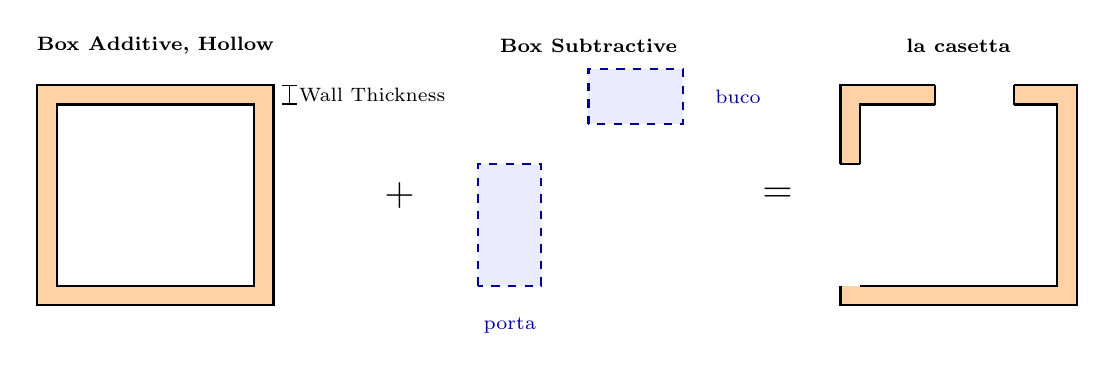
\begin{tikzpicture}[font=\footnotesize, x=1cm, y=1cm]
  % box additiva hollow (sezione)
  \node[font=\scriptsize\bfseries] at (1.5,3.3) {Box Additive, Hollow};
  \fill[orange!35] (0,0) rectangle (3,2.8);
  \fill[white] (0.25,0.25) rectangle (2.75,2.55);
  \draw[thick] (0,0) rectangle (3,2.8); \draw[thick] (0.25,0.25) rectangle (2.75,2.55);
  \draw[|-|, thin] (3.2,2.55) -- node[right, font=\scriptsize]{Wall Thickness} (3.2,2.8);
  \node at (4.6,1.4) {\Large $+$};
  % sottrattive
  \node[font=\scriptsize\bfseries] at (7.0,3.3) {Box Subtractive};
  \draw[thick, dashed, blue!60!black, fill=blue!8] (5.6,0.25) rectangle (6.4,1.8);
  \node[font=\scriptsize, blue!60!black] at (6.0,-0.25) {porta};
  \draw[thick, dashed, blue!60!black, fill=blue!8] (7.0,2.3) rectangle (8.2,3.0);
  \node[font=\scriptsize, blue!60!black] at (8.9,2.65) {buco};
  \node at (9.4,1.4) {\Large $=$};
  % risultato
  \begin{scope}[xshift=10.2cm]
    \node[font=\scriptsize\bfseries] at (1.5,3.3) {la casetta};
    \fill[orange!35] (0,0) rectangle (3,2.8);
    \fill[white] (0.25,0.25) rectangle (2.75,2.55);
    \fill[white] (-0.05,0.25) rectangle (0.3,1.8);
    \fill[white] (1.2,2.5) rectangle (2.2,2.85);
    \draw[thick] (0,1.8) -- (0,2.8) -- (1.2,2.8); \draw[thick] (2.2,2.8) -- (3,2.8) -- (3,0) -- (0,0) -- (0,0.25);
    \draw[thick] (0.25,1.8) -- (0.25,2.55) -- (1.2,2.55); \draw[thick] (2.2,2.55) -- (2.75,2.55) -- (2.75,0.25) -- (0.25,0.25);
    \draw[thick] (0,1.8) -- (0.25,1.8); \draw[thick] (1.2,2.55) -- (1.2,2.8); \draw[thick] (2.2,2.55) -- (2.2,2.8);
  \end{scope}
\end{tikzpicture}
\caption{Additive e Subtractive in sezione: una box additiva vuota (Hollow, con il suo
Wall Thickness) e due box sottrattive che la ``bucano'', una per la porta e una per il
buco sul soffitto da cui cadere nella stanza sottostante, come nella casetta costruita a
lezione. Ricostruzione schematica; le proporzioni sono indicative.}
\label{ue13:fig:csg}
\end{figure}

\paragraph{Il però: le brush sono pesanti.} ``Ora c'è un però, e il però è che le brush
sono \textbf{pesanti}.'' Se si riempie una scena di brush, ``perché volete diverse casette e
diverse zone dentro cui entrare'', ``si carica tanto sulla memoria del progetto''. Il
rimedio: \textbf{farla diventare una static mesh}. Nei Details della brush c'è il comando
per creare una static mesh dalla geometria (\emph{Create Static Mesh}, nella parte avanzata
dei Brush Settings), che chiede dove salvarla. Il docente lo fa con la casetta: nel
Content Browser compare ``un bloccone'', ma solo della brush selezionata (``se avessimo
selezionato tutte quante le brush, avremmo avuto un effetto diverso'': la mesh le avrebbe
comprese tutte). Il docente elimina la brush originale, ``non ci serve più'': la static mesh
che resta ``è molto meno pesante. Io posso riempirci la scena di questa roba qua.''
Bisognerebbe solo sistemarne il \textbf{pivot}, ``perché ce l'ho salvato col pivot
strano''. Un consiglio di ordine: invece di ``buttarla qui in mezzo al Content'', come ha
fatto lui, create ``una \emph{new folder} che chiamate, che ne so, \textbf{Blockout
Assets}'', e lì dentro mettete tutto quello che create. (Poi le elimina: a lui non servono.)

\paragraph{Approfondimento: perché le brush pesano, e Create Static Mesh.} Le geometry
brush sono la versione moderna della geometria \textbf{BSP} (\emph{binary space
partitioning}) delle vecchie versioni di Unreal: le brush additive e sottrattive vengono
combinate, nell'ordine in cui sono state create, in un'unica geometria del livello, che
l'editor ricalcola (\emph{Build Geometry}) quando le si modifica. Questa geometria non si
può istanziare, non ha LOD, ha UV e lightmap generate automaticamente e la sua collisione
è meno efficiente di quella di una mesh: per questo, oltre che per la memoria, Epic
raccomanda di usarle per il block out e di convertirle (o sostituirle) con static mesh
nel livello finale. Il comando \textbf{Create Static Mesh} salva la geometria delle brush
selezionate come asset \emph{Static Mesh}, con i materiali delle facce come slot; la
mesh nasce con il pivot all'origine del mondo o della prima brush, che si corregge con il
\emph{Modeling Mode} (strumento \emph{Pivot}) o riposizionandola. Nel libro di Romero e
Sewell le brush non compaiono: il libro costruisce i livelli con static mesh duplicate
(capitolo 9, il pavimento duplicato con Alt e trascinamento per raddoppiare l'area di
gioco). Quanto al modeling tool, il \emph{Modeling Mode} esisteva già come plugin
sperimentale nelle ultime versioni di Unreal~4, ma è con Unreal~5 che è diventato uno
strumento standard dell'editor: la frase del docente è vera nella sostanza. Funzionamento
generale dell'engine, salvo il riferimento al libro.

% ---------------------------------------------------------------------
\section{Le altre forme e il Brush Editing}
\label{ue13:sec:forme}

``Vediamo effettivamente cosa ci permettono di fare le altre brush.'' (La box sottrattiva il
docente se la tiene, ``almeno vediamo''.)

\paragraph{Cone.} Ha sempre le stesse impostazioni per le facce. Nei Brush Settings: un
valore \textbf{Z}, l'altezza; un \textbf{Outer Radius}; un \textbf{Inner Radius}, che non
si può modificare finché il cono non è \textbf{Hollow}: ``se io la rendo vuota'' si vede
com'è dentro, e si crea una struttura ``sulla base di quello che a me serve''. Il docente ci
mette dentro la box sottrattiva: ``una capannola mezza favola, una tenda''. Si può aumentare
il numero di lati (\textbf{Sides}): da 3, ``una piramide, anzi un D4'', fino a 500. A 500
``ha un po' stutterato, e non ci sarà mai un momento in cui ti servirà avere un cono così
preciso'', ma più facce lo rendono ``un po' più smussato''.

\paragraph{Cylinder.} ``Più o meno le stesse cose'': l'altezza, l'Outer Radius (``quanto è
largo effettivamente''), le facce come per il cono, Hollow o no, e il tipo, additivo o
sottrattivo.

\paragraph{Sphere.} Il \textbf{Radius}, ``quanto è ampia'', e la \textbf{Tessellation},
``quanti blocchi ha, quindi quanto è sferica''.

\paragraph{Linear Stair.} Tutto si basa sullo scalino, ``come anche le altre scale'': la
lunghezza del singolo scalino (\textbf{Step Length}), l'altezza (\textbf{Step Height}), la
larghezza (\textbf{Step Width}) e il numero di scalini (\textbf{Num Steps}): ``aumentando
gli scalini, aumenta l'altezza e aumenta la distanza''. Poi \textbf{Add to First Step},
``quanto in alto in più deve essere il primo scalino'': ``vedete, lui alza un tot''.

\paragraph{Curved Stair.} Altezza e larghezza dello scalino, e in più:
\begin{itemize}
  \item l'\textbf{Inner Radius}, il raggio del cerchio interno: ``se è molto largo, le
        scale vengono più arcuate'';
  \item l'\textbf{Angle of Curve}, ``quanto deve curvare la scala'': di default 90 gradi,
        ``però potreste fare anche 180, 270, anche 360 gradi'', se volete ``una singola
        chiocciola'';
  \item Num Steps e Add to First Step, ``esattamente allo stesso modo'';
  \item \textbf{Counter Clockwise}, per le scale ``che vanno nell'altra direzione''.
\end{itemize}
``Con tutte queste, poi potete andare a creare effettivamente delle static mesh.''

\paragraph{Spiral Stair.} ``Gli stessi parametri'': Inner Radius, Step Width, Step Height,
e in più lo spessore del singolo gradino (\textbf{Step Thickness}), ``perché è costruita
proprio a gradoni, ognuno di questi è un oggetto a sé stante, tutti attaccati l'uno con
l'altro''. C'è poi il numero di scalini \emph{per 360 gradi} (\textbf{Num Steps Per 360}):
``se voi dite che devono esserci 33 scalini per fare 360 gradi, poi dovete aggiungere
abbastanza scalini per arrivare a fare 360 gradi''; abbassandolo, con lo stesso numero
totale di scalini (``50, 60'') ne servono meno per fare un giro. Infine si può rendere
liscio il soffitto (\textbf{Sloped Ceiling}) o il pavimento (\textbf{Sloped Floor}), ``e
quindi avere una sorta di scivolo, una rampa'', e Counter Clockwise.

\paragraph{Il Brush Editing.} ``Prima facciamo un'ultima roba'': passare dalla
\textbf{Selection Mode} al \textbf{Brush Editing} (dal menu delle modalità dell'editor). Qui
si fanno ``piccole operazioni di modellazione'': selezionare un \textbf{vertice} e
spostarlo, una \textbf{faccia} e muoverla, un \textbf{edge} e muoverlo, ``in questo modo ci
andiamo a creare esattamente il tipo d'oggetto che serve a noi, anche se la forma che
serve a noi non c'era'' fra le brush. E lo \textbf{Split}: ``fa passare una serie di
vertici e di edge a tagliare'', una sezione dell'oggetto; ``si formano nuove facce, e
queste nuove facce possono essere prese e modificate''. ``Non so quanto spesso vi tornerà
utile fare un ecomostro del genere, però avete la possibilità di farlo.'' Un'avvertenza
emersa dalla prova: dopo le modifiche, l'oggetto ``è ancora una brush'', ma ``appena
l'andiamo a modificare'' dai Brush Settings ``ritorna come era precedentemente'': i
parametri ricostruiscono la forma da zero e cancellano le modifiche manuali.

\begin{table}[htbp]
\centering
\small
\begin{tabular}{@{}p{2.5cm}p{11.5cm}@{}}
\toprule
\textbf{Brush} & \textbf{Parametri (Brush Settings)} \\
\midrule
tutte & Brush Type: Additive / Subtractive; i materiali e le UV si impostano per faccia \\
Box & X, Y, Z; Wall Thickness (default 10); Hollow; Tessellated (solo se non hollow) \\
Cone & Z (altezza); Cap Z; Outer Radius; Inner Radius (solo se hollow); Sides (da 3 a
500); Align to Side; Hollow \\
Cylinder & Z; Outer Radius; Inner Radius (solo se hollow); Sides; Align to Side; Hollow \\
Sphere & Radius; Tessellation \\
Linear Stair & Step Length; Step Height; Step Width; Num Steps; Add to First Step \\
Curved Stair & Inner Radius; Step Height; Step Width; Angle of Curve (default
90$^\circ$); Num Steps; Add to First Step; Counter Clockwise \\
Spiral Stair & Inner Radius; Step Width; Step Height; Step Thickness; Num Steps Per 360;
Num Steps; Sloped Ceiling; Sloped Floor; Counter Clockwise \\
\bottomrule
\end{tabular}
\caption{Le geometry brush e i loro parametri. I nomi sono quelli dei Details di Unreal
Engine~5; quelli non letti a lezione (Cap Z, Align to Side) sono completati come
approfondimento.}
\label{ue13:tab:brush}
\end{table}

``Sono le cinque e mezza.'' Il docente annuncia che, al ritorno dalla pausa, si potrebbe
fare ``un piccolo block out utilizzando gli oggetti che avete'': le brush, le static mesh e
gli oggetti fatti con Igor, ``per cui magari vi piazzate dei collectible da raggiungere in
giro'', ``anche molto semplice''. Pausa di un quarto d'ora: ``facciamo 45''.

% ---------------------------------------------------------------------
\section{La pausa e la scelta del formato}
\label{ue13:sec:pausa}

(Durante la pausa la trascrizione contiene solo il blocco di testo ripetuto citato
nell'introduzione.) Alla ripresa c'è un problema di volume (``stavo leggendo il messaggio
che aveva scritto Augusto in chat'') e l'appello: Federico c'è, Guido ``c'è, ma non gli
funziona la telecamera'' (``basta che siete responsivi'').

\paragraph{La domanda del docente.} ``Ci stavo pensando adesso che stavamo fermi'': come
preferiscono strutturare le lezioni?
\begin{enumerate}
  \item una prima parte di spiegazione e una seconda in cui gli studenti ``provano a
        costruire qualcosa'', magari in streaming, ``così gli altri vedono anche cosa
        fate'' e il docente può commentare;
  \item tutte e tre le ore di spiegazione, con il lavoro pratico fra una lezione e l'altra
        e i feedback all'inizio della lezione successiva. Il tempo a disposizione cambia:
        ``da oggi, che è giovedì, fino a martedì avrete più tempo; da martedì a giovedì ne
        avrete meno''.
\end{enumerate}
Un primo studente preferisce la prima opzione, ``perché almeno abbiamo dei feedback diretti
e ci si può soffermare di più sulle varie cose''. Un altro la seconda, ``perché forse
riusciamo a fare più cose'', ``vediamo un po' più di argomenti''. Il docente avverte che le
cose che si faranno con lui ``sono tendenzialmente non troppo complesse, è più una
questione di metterle assieme'', e che non vorrebbe la situazione in cui ``io vi dico
facciamo questa cosa, la prossima volta me lo fate vedere e nessuno fa niente''. Edoardo,
alle prese con il caldo, dice che fare le cose fra una lezione e l'altra ``non è un peso''
se trova una soluzione; un altro: ``personalmente mi piace la seconda''. Il voto (``siete
dispari, quindi uscirà fuori una verità o l'altra''; ``per chi ci guarda da casa sarà tutto
in mano alle persone che erano qui'') premia la \textbf{seconda}: ``Tommaso, indipendentemente
dal tuo input, il popolo ha deciso di riempire la lezione con delle cose che magari faccio
io''.

Conseguenze: la lezione sullo \textbf{speed level design} andrà ``rimaneggiata'', ``perché
non so quanto ha senso che io mi metta a fare uno speed level per tre ore con voi che mi
guardate''; era ``una roba che mi sarebbe piaciuto far fare a voi''. Per la volta successiva,
a chi vuole, il docente chiede ``un piccolo livellino'' con geometrie e static mesh, ``per
giocare un po''': ``è molto bello sapere come funziona Unreal, però deve esserci del
\textbf{divertimento} nella creazione. Io mi devo divertire mentre creo il gioco.'' Le
indicazioni precise arrivano a fine lezione (sezione~\ref{ue13:sec:compiti}).

\paragraph{Che cosa fare nell'ora rimasta.} Personalizzare i parametri del bot in una gym
``è relativamente fine a se stesso'', ``un discorso abbastanza semplice'' che gli studenti
possono fare da soli. Meglio un altro actor interessante: le \textbf{luci}, e ``se riesco,
un accennino di post process''. Le luci si vedranno ``in un vuoto'', ``senza un dressing già
finito'', e si riprenderanno quando si parlerà di \emph{enrichment}, di dressing e di
ambienti, con lo speed level; per quella lezione il docente potrebbe preparare
``un ambientino'' o passare un pacchetto, ``così chi vuole lo fa assieme a me''. Le slide
non servono: ``faremo a braccio''. (Di nuovo problemi con Zoom: ``ogni volta che parto con la
stream non funziona il tasto destro''.) Il docente costruisce con una grande box un
ambientino chiuso (``così abbiamo un po' d'ombra''), invitando Filippo, che preferiva fare
le cose insieme, a sperimentare in parallelo. (Una parte della costruzione, nella
trascrizione, è incomprensibile: ``me la metà? E questa la facciamo? Giusto per fare
razzola''.)

% ---------------------------------------------------------------------
\section{Le luci: i tipi e la mobility}
\label{ue13:sec:mobility}

``Cos'è che non sta più funzionando in quella zona lì?'' Dentro la box: ``la luce del sole'',
risponde uno studente. La luce del sole è un tipo di luce, ``la signora
\textbf{Directional Light}''. Le luci di Unreal sono cinque: \textbf{Directional},
\textbf{Point}, \textbf{Spot}, \textbf{Rect} e \textbf{Sky Light}. Secondo la classificazione
del docente:
\begin{itemize}
  \item directional e sky light sono \textbf{luci ambientali};
  \item point e spot light si usano ``principalmente per l'illuminazione'';
  \item la rect light ``principalmente per i riflessi o per delle luci specifiche''.
\end{itemize}

\paragraph{Il costo dei rimbalzi.} ``Una cosa importante da dire è che il modo in cui Unreal
calcola le luci è simulando delle onde'' e il modo in cui ``queste onde luminose rimbalzano
sulle superfici''. Ci saranno situazioni in cui a una luce verranno chiesti ``troppi
rimbalzi, che equivalgono a troppi calcoli, che equivalgono a un peso molto elevato'':
bisogna stare attenti a come si posizionano le luci. (Sull'idea delle ``onde'' si veda
l'approfondimento alla fine della sezione.)

\paragraph{La Mobility.} ``Un parametro fondamentale che c'è in tutte le luci'' è la
\textbf{Mobility}: di default le luci sono \textbf{Stationary}, ma ci sono anche
\textbf{Static} e \textbf{Movable}. ``Non mi aspetto una risposta super completa, voglio
vedere se riusciamo ad arrivarci'' (``basta che ci passate sopra col mouse e ve lo dice
cosa fanno, però state con me''). Le ipotesi degli studenti: movable ``sarà tipo la luce di
una macchina''; stazionaria ``che sta ferma e non si muove'', ma statica ``mi sembra simile
come significato''; un altro propone ``statica un lampione, stazionaria il faro di una
macchina ferma, che potenzialmente si può muovere''; un altro ancora che la movable
``dovrebbe avere delle proprietà fisiche, magari condizionata dalla gravità'' (``la gravità
non c'entra''); un altro l'angolazione (``no, l'angolazione dipende dal tipo di luce che
utilizziamo''). Il docente rinuncia alla prova pratica (``qui c'è un po' di fregatura,
perché siamo in preview'') e parte dagli usi:
\begin{itemize}
  \item una luce \textbf{movable} è quella di ``una torcia a mano'', di una torcia
        elettrica che si punta, dei fari di una macchina, delle luci di un aereo: ``qualcosa
        in movimento'';
  \item una luce \textbf{stazionaria} è quella di un lampione, di un soffitto, ``di una
        qualsiasi luce di una casa'' \emph{dentro} il livello;
  \item una luce \textbf{statica} serve agli stessi scopi della stazionaria, ``ma fuori dal
        vostro livello''.
\end{itemize}
``Cosa cambia fra statica e stazionaria?'' Uno studente: ``nella stazionaria ci può
interagire un actor come il character''. ``Esatto.'' Le proprietà sono due: se si muove la
luce, l'ambiente reagisce?; se si passa davanti alla luce, la luce reagisce?
(figura~\ref{ue13:fig:mobility}):
\begin{itemize}
  \item la luce \textbf{statica} ``viene cucinata sulla scena'': è \emph{baked}
        completamente nell'editor e non si può modificare in gioco. Quando si
        \emph{buildano} le luci o si esporta il livello, ``la luce viene bakeata ed è
        impressa sulla scena''. Se si sposta l'actor della luce, la luce ``rimane dove è
        stata bakeata''; se il character ci passa davanti, la luce non reagisce. Si usa ``in
        tutti quei posti in cui so che non avrà interazioni e sarà soltanto luce
        d'atmosfera, luce d'ambiente''. È ``il tipo di luce più leggero'';
  \item la luce \textbf{stazionaria} ``se la muovo si rompe, ma se sta ferma e io ci passo
        davanti interagisce con me'': il character proietta ombre corrette, ma se si sposta
        la luce dopo il bake, la luce non si aggiorna;
  \item la luce \textbf{movable} ``fa entrambe le cose'': è completamente dinamica, reagisce
        agli oggetti e può essere spostata ``senza nessun problema''.
\end{itemize}

\begin{figure}[htbp]
\centering
\begin{tikzpicture}[font=\footnotesize, x=1cm, y=1cm,
  ue13col/.style={draw, thick, rounded corners=3pt, minimum width=4.0cm, minimum height=0.8cm,
                  align=center}]
  \node[ue13col, fill=gray!15] (st) at (0,0) {\textbf{Static}};
  \node[ue13col, fill=yellow!30] (sy) at (4.6,0) {\textbf{Stationary} (default)};
  \node[ue13col, fill=orange!30] (mv) at (9.2,0) {\textbf{Movable}};
  \node[align=left, anchor=north, text width=4.0cm] at (0,-0.6)
    {\textbf{bake}: sì, tutta\\ \textbf{si sposta in gioco}: no\\ \textbf{ombre dei personaggi}: no\\
     \textbf{costo}: il più basso\\[2pt] \emph{luce d'ambiente fuori dall'area di gioco}};
  \node[align=left, anchor=north, text width=4.0cm] at (4.6,-0.6)
    {\textbf{bake}: sì, la parte fissa\\ \textbf{si sposta in gioco}: no\\ \textbf{ombre dei personaggi}: sì\\
     \textbf{costo}: medio\\[2pt] \emph{lampioni, luci di casa, soffitti}};
  \node[align=left, anchor=north, text width=4.0cm] at (9.2,-0.6)
    {\textbf{bake}: no\\ \textbf{si sposta in gioco}: sì\\ \textbf{ombre dei personaggi}: sì\\
     \textbf{costo}: il più alto\\[2pt] \emph{torce, fari, luci di un aereo}};
  \draw[-{Stealth[length=2.5mm]}, very thick, gray] (-2.0,-3.3) -- node[below, font=\scriptsize]{più dinamica, più pesante} (11.2,-3.3);
\end{tikzpicture}
\caption{Le tre Mobility delle luci come le descrive il docente: che cosa viene
precalcolato (\emph{baked}), se la luce si può spostare in gioco, se reagisce ai personaggi
che le passano davanti, quanto pesa e per che cosa si usa.}
\label{ue13:fig:mobility}
\end{figure}

\paragraph{Approfondimento: onde, raggi e Lumen.} L'immagine delle ``onde'' è una
semplificazione del docente: Unreal non simula la luce come un'onda (niente interferenza o
diffrazione), ma come energia che viaggia in linea retta e rimbalza, cioè per
\emph{raggi}. Il calcolo dei rimbalzi (l'illuminazione \emph{globale}) avviene in due modi:
precalcolato, con \textbf{Lightmass}, che scrive il risultato nelle \emph{lightmap} delle
superfici al momento del build (luci static e stationary); o in tempo reale, con
\textbf{Lumen}, il sistema di illuminazione globale dinamica che Unreal Engine~5 attiva di
default nei progetti nuovi. Il principio del docente resta valido: più superfici e più
luci si sovrappongono, più calcoli servono, che siano fatti una volta nel build o a ogni
frame. Sulla stationary, un dettaglio in più: in gioco se ne possono cambiare colore e
intensità (non la posizione), e le ombre che proietta sugli oggetti fermi sono precalcolate,
mentre quelle degli oggetti in movimento sono dinamiche. Romero e Sewell (capitolo 4)
mettono la \emph{Mobility} di una point light a \textbf{Movable} proprio ``per poter
cambiare le proprietà della luce durante l'esecuzione'', quando la accendono e la spengono
da Blueprint. Funzionamento generale dell'engine, salvo il riferimento al libro.

% ---------------------------------------------------------------------
\section{La directional light e la sky light}
\label{ue13:sec:directional}

Il docente porta la directional light e la sky light ``tutte nello stesso posto''.
``Spostare queste luci non ha nessun tipo d'effetto.'' Perché?

\paragraph{La Directional Light.} Si può muoverla e scalarla ``come voglio e non cambia
assolutamente nulla. Ma se la ruoto, la luce reagisce.'' (``In questo caso reagisce anche''
un altro actor del cielo, ``perché è collegato'': la trascrizione dice ``la Schakespeare'' e
``la Schiapunsky'', con ogni probabilità la \emph{Sky Sphere} o la \emph{Sky Atmosphere}
del livello; il nome esatto non è ricostruibile.) La ragione: ``la directional light è
composta in una maniera abbastanza peculiare: è un \textbf{fascio di rette parallele} che
prende tutta la scena''. Spostarla non cambia nulla; ruotarla cambia ``il modo in cui viene
indirizzata la luminosità''. I parametri interessanti:
\begin{itemize}
  \item l'\textbf{Intensity}: aumentandola, ``va in questo caso a bruciare un pochino tutta la
        scena'' (``l'intensità della luce calcolata in X'': l'unità di misura nella
        trascrizione è incomprensibile; per la directional è il \emph{lux});
  \item il \textbf{Light Color}: una ruota dei colori per il colore della luce, la sua
        saturazione, ``quanto sarà scura, magari quanto sarà livida''. Se si vuole che più
        luci abbiano lo stesso colore, si copia il codice \textbf{Hex Linear} e lo si incolla
        nelle altre, ``il modo più comodo piuttosto che cercare a mano di replicare la stessa
        luce'': per esempio un corridoio in cui tutte le torce sono ``molto calde, molto
        accese, molto infuocate'';
  \item la \textbf{Temperature} (con \emph{Use Temperature}), per una luce ``tendenzialmente
        più calda o più fredda''; ``così, se volete fare \emph{Breaking Bad} quando sono in
        Messico, tutto giallo'';
  \item \textbf{Affects World}: ``questa luce che sto utilizzando ha effetto sul mondo? È una
        luce attiva o disabilitata?''. Serve, per esempio, a vedere ``come contribuisce alla
        scena'' una luce alla volta;
  \item \textbf{Cast Shadows}: la luce illumina comunque, ma proietta le ombre solo se è
        attivo;
  \item la \textbf{Dynamic Shadow Distance}: secondo il docente, ``quanto precisamente
        viene calcolata l'ombra, quanto è netta''. ``Non può essere notato adesso perché
        stiamo utilizzando solo geometrie''; con asset veri un valore basso si nota. Il
        docente cerca nel progetto una mappa già arredata per mostrarlo (``mi sa che non ne
        abbiamo, a parte quelle che ha fatto Igor'') e rimanda: ``la prossima volta mi
        preparo una scenetta carina a livello estetico''. È un parametro che ``tende ad
        appesantire un pochino le scene'', ma ``l'effetto che fa è talmente meglio rispetto a
        non averlo'': ``giocatevi un po' di potenza in più''.
\end{itemize}

\paragraph{Una sola per scena.} ``Non dovete mai avere \textbf{due directional} nella stessa
scena'': l'engine prova a calcolarle entrambe, ``fa molta fatica'' e ``il risultato è
tremendo'', con problemi di ombre calcolate in direzioni diverse. Allo stesso modo
``evitate di avere due sky sphere'', anzi, si corregge, due \textbf{sky light}: ``skylight e
directional light, una soltanto per scena''.

\paragraph{La Sky Light.} ``Funziona in maniera un po' diversa'', ``un po' più complessa'', e
``al momento non ci serve troppo indagarla''. Che cosa fa: ``è la luce che dà il
\textbf{mood}, la diffusione'', ``va a colorare l'aria, va a dare colore alla scena''. Si vede
cambiando il colore della sky light: cambiano di colore le \emph{ombre}. Per una scena al
tramonto, ``piuttosto che avere solo la directional che è arancione'', si media fra
directional e sky light, ``più tutta una serie di altre cose, perché utilizzeremo anche il
post process'' (la volta successiva). Fra i parametri, oltre all'intensità, quelli
dell'\textbf{ambient occlusion}: la distanza massima (\emph{Occlusion Max Distance}), il
contrasto (\emph{Contrast}) e ``quanto è moltiplicata'' (\emph{Occlusion Exponent} e
\emph{Min Occlusion}); e anche qui Cast Shadows e Affects World. ``Principalmente, mood
della scena e ambient occlusion.''

\paragraph{Approfondimento: Dynamic Shadow Distance, e due directional.} Il nome completo
del parametro è \emph{Dynamic Shadow Distance Movable Light} (o \emph{Stationary Light}, a
seconda della mobility): è la distanza dalla camera entro cui la directional disegna le
ombre dinamiche, divise in \emph{cascate} (\emph{Cascaded Shadow Maps}) di risoluzione
decrescente. Non è quindi la ``nettezza'' in sé, ma lo spazio su cui la risoluzione delle
ombre viene distribuita: oltre quella distanza le ombre dinamiche spariscono (restano solo
quelle precalcolate), e allungarla, a parità di cascate, rende le ombre vicine meno
dettagliate. In Unreal Engine~5, con le \emph{Virtual Shadow Maps} attive di default, questo
compromesso pesa molto meno. Sulle due directional, la regola del docente è la pratica
comune; a rigore Unreal ne supporta due solo come sole e luna dell'atmosfera (indice
\emph{Atmosphere Sun Light Index} 0 e 1), un caso particolare. Funzionamento generale
dell'engine.

% ---------------------------------------------------------------------
\section{Point light e spot light}
\label{ue13:sec:point}

``Passando a delle luci con cui andrete a smanettare molto ma molto di più'': le luci
``antropiche'', quelle che si useranno ``per fare quasi tutto'', \textbf{point light} e
\textbf{spot light}. ``Fra le due, qual è più leggera, più facile da calcolare,
indipendentemente dalla mobility?''

\paragraph{La domanda.} Uno studente risponde la point light, ``perché non si va a calcolare
anche la direzione''. ``È esattamente il contrario.'' La point light è a 360 gradi: ``lui
calcola contemporaneamente tutte le direzioni''. La \textbf{spot light} è più leggera
``perché non va a calcolare i rimbalzi della luce nelle altre direzioni'': ``la discriminante
è quella della direzione''. In una scena affollata, la spot illumina solo dove la si punta,
mentre la point ``va posizionata con attenzione perché va a colpire anche gli oggetti che ha
alle spalle'', ``indiscriminatamente dalla direzione''.

\paragraph{L'Attenuation Radius.} Per la point light, ``i due parametri più importanti sono
l'intensità e l'\textbf{Attenuation Radius}'', la sfera che si vede attorno alla luce.
``Indipendentemente dal fatto che io ho messo 10.000 miliardi di intensità, se il raggio non
tocca nulla la luce non illumina'' (o meglio, illumina solo dentro la sfera, ``quindi non
rimbalza su niente''). È ``il raggio massimo entro cui la luce avrà effetto'', e gestisce
un'attenuazione dalla sorgente fino al bordo: il \emph{gradiente} della luce. Con
un'intensità altissima, per un'attenuazione sensata bisogna ingrandire molto il raggio. Ma
anche con un'intensità bassa l'attenuazione arriva fino al bordo, e questo è il punto: il
raggio è ``il parametro che va gestito con attenzione'', ``perché determina con quanti
oggetti la luce andrà a compenetrare'', e quindi quante ombre dovrà proiettare. ``Anche se
l'intensità è molto bassa, nel momento in cui questo muro è all'interno del raggio,
l'engine dovrà calcolare'' l'ombra e la luce su quella superficie.

\paragraph{La X rossa.} ``Una cosa che vi capiterà sicuramente'': una luce con una
\textbf{X rossa} sopra. Il docente la riproduce mettendo più luci vicine (al primo tentativo
``non abbastanza'': i raggi erano piccoli). Vuol dire che ``l'engine ha rinunciato a far
proiettare ombre a questa luce'': la luce illumina comunque, ``ma non proietta ombre perché
ci sono troppe altre luci con cui questa luce sta compenetrando''. L'engine lo segnala come
problema, ``non grave''. I rimedi sono due: dire noi alla luce di non proiettare ombre
(Cast Shadows disattivato), così l'engine ``non cercherà costantemente di proiettarle'';
oppure \textbf{ridurre il raggio} ``a tal punto da non farlo compenetrare con troppe cose''.
``Non riempite la vostra scena di luci, piuttosto utilizzate \textbf{poche luci molto
significative}.''

\paragraph{Il corridoio.} L'esempio: un corridoio con una fila di luci. Mentre il
personaggio passa, le ombre sono corrette ``fino a che non arriviamo qui vicino'': lì la
luce viene calcolata ``come se questa non ci fosse'', e l'ombra viene proiettata dalle due
luci ai lati. ``Vedete, qui skippa, qui salta'': l'ombra della luce con la X non c'è, c'è
solo quella della luce ``un po' più lontana'', mentre altrove l'ombra è ``molto più forte,
molto più precisa, molto più netta''. ``Se replicate questo esperimento per conto vostro, vi
rendete conto che è abbastanza semplice da replicare.''

\paragraph{La sorgente: Source Radius, Soft Source Radius, Source Length.} Come illuminare
un corridoio ``piuttosto che avere una luce per torcia, una luce per punto''? Si modifica la
\textbf{sorgente}: ingrandendo il \textbf{Source Radius} e allungando la \textbf{Source
Length}, la luce non parte più da un punto ma ``da un cilindro, da una capsula'', ed è
``più distribuita''. Il raggio può anche essere zero, ``se volete una linea e basta''. È
così che si fanno illuminazioni particolari, ``tipo un locale illuminato unicamente dalla
luce dei \textbf{neon}'': mesh con materiali \textbf{emissive}, ``che quindi già emettono una
piccola luce di loro'', più luci distribuite ``in maniera più omogenea'' in questo modo. Il
\textbf{Soft Source Radius} ``serve per creare un'altra lucina interna, come quando puntate
una torcia verso il muro'': una parte più attenuata all'esterno e una meno attenuata
all'interno (``si vede meglio con la spot''; il docente non riesce a mostrarlo bene). Più
sotto ci sono di nuovo Affects World e Cast Shadows, e lo \emph{scattering} con la nebbia
volumetrica (\emph{Volumetric Scattering Intensity}), che servirà quando si userà una
nebbia (la trascrizione dice ``una FOD'', con ogni probabilità \emph{fog}); poi ``molti, molti
parametri'' per le ombre (risoluzione, comportamento sulle pendenze). ``Non tutti vi
servono'', ``a meno che non vogliate fare proprio il \emph{light artist}''. (``Non l'ho
detto prima'': anche la point light ha il Light Color, ``per fare le vostre luci da inferno,
da nightclub, da \emph{Night City}''.)

\paragraph{La spot light.} È fatta a \textbf{cono}, quindi si ruota. Intensità e Light
Color come le altre; l'\textbf{Attenuation Radius}, qui, ``non dipende da quanto è la
sfera, ma è la lunghezza del cono'', ``quanto in là viene proiettata'': ``se sta così non
colpisce il muro, così illumina questa parte del muro''. Poi due angoli
(figura~\ref{ue13:fig:luci}):
\begin{itemize}
  \item l'\textbf{Outer Cone Angle}, che gestisce il cono;
  \item l'\textbf{Inner Cone Angle}, il cono interno, ``l'effetto torcia'': nella parte
        colpita dall'inner cone ``ci sarà una minore attenuazione''. Con i due angoli vicini
        il bordo è netto; ``volendo potete avere anche un cono che non attenua mai alla
        base, che attenua soltanto sulla distanza''. Questo cono serve a determinare la
        \emph{sfumatura}, ``ed è anche quello che faceva l'altro nella point, ma con questo
        si nota meglio''.
\end{itemize}
Anche qui Source Radius, Source Length e Soft Source Radius, e i parametri delle ombre.

\paragraph{La domanda sull'effetto accecante.} Uno studente chiede se, guardando
direttamente la luce, ci sia ``l'effetto accecante''. ``No, assolutamente no.'' L'effetto
``tipo quando guardi il sole'' si crea con il \textbf{post process}, che il docente vuole
far vedere ``quando abbiamo una mappa che non sia soltanto delle geometrie'' (con un
pacchetto di mesh e mappe già fatte: ``sono abbastanza sicuro che questo pacchetto dovesse
avere delle mappe''). Con i parametri del post process si aggiungono \textbf{bloom} e
\textbf{lens flare}. Altro esempio: i \textbf{god rays} (``god shaft''), ``una luce molto
forte che entra dalla finestra e c'è questa proiezione luminosa che taglia la scena''.
``Quella roba lì con la luce non puoi farla. Ti serve la luce, ma devi andare a manipolare
il modo in cui la telecamera vede la luce con la post produzione.'' Per questo ``la post
produzione va fatta dopo le luci'': ``prende l'illuminazione della scena e ci aggiunge delle
lenti, degli effetti''. Fra le ``lenti'', oltre al bloom: la messa a fuoco, la distorsione,
la \emph{chromatic aberration}.

\begin{figure}[htbp]
\centering
\begin{tikzpicture}[font=\footnotesize, x=1cm, y=1cm]
  % point light
  \node[font=\scriptsize\bfseries] at (1.6,3.4) {Point Light};
  \shade[inner color=yellow!70, outer color=white] (1.6,1.6) circle (1.5);
  \draw[dashed, thick, orange!70!black] (1.6,1.6) circle (1.5);
  \fill[orange] (1.6,1.6) circle (0.08);
  \draw[-{Stealth[length=1.6mm]}] (1.6,1.6) -- (2.66,2.66);
  \node[font=\scriptsize, align=center] at (1.6,-0.5) {Attenuation Radius = sfera;\\360$^\circ$: colpisce anche\\ciò che ha alle spalle};
  % spot light
  \begin{scope}[xshift=4.4cm]
    \node[font=\scriptsize\bfseries] at (1.6,3.4) {Spot Light};
    \fill[yellow!25] (0.2,2.8) -- (3.2,0.2) -- (0.9,0.0) -- cycle;
    \fill[yellow!65] (0.2,2.8) -- (2.55,0.4) -- (1.55,0.1) -- cycle;
    \draw[dashed, thick, orange!70!black] (0.2,2.8) -- (3.2,0.2);
    \draw[dashed, thick, orange!70!black] (0.2,2.8) -- (0.9,0.0);
    \fill[orange] (0.2,2.8) circle (0.08);
    \node[font=\scriptsize, anchor=west] at (2.7,1.3) {Outer Cone};
    \node[font=\scriptsize, anchor=west, fill=white, inner sep=1pt] at (1.25,1.15) {Inner};
    \node[font=\scriptsize, align=center] at (1.6,-0.5) {Attenuation Radius =\\lunghezza del cono};
  \end{scope}
  % rect light
  \begin{scope}[xshift=8.8cm]
    \node[font=\scriptsize\bfseries] at (1.8,3.4) {Rect Light};
    \fill[yellow!30] (0.9,2.4) -- (2.7,2.4) -- (3.4,0.2) -- (0.2,0.2) -- cycle;
    \draw[very thick, fill=orange!60] (0.9,2.4) rectangle (2.7,2.6);
    \draw[very thick, gray!70!black] (0.9,2.4) -- (0.55,1.95);
    \draw[very thick, gray!70!black] (2.7,2.4) -- (3.05,1.95);
    \node[font=\scriptsize, anchor=east] at (0.55,2.0) {Barn Door};
    \node[font=\scriptsize, align=center] at (1.8,-0.5) {Source Width $\times$ Height;\\Barn Door Angle e Length};
  \end{scope}
\end{tikzpicture}
\caption{Le tre luci locali e i parametri che ne determinano la forma: la sfera di
attenuazione della point light, i due coni della spot light (nel cono interno
l'attenuazione è minore) e la sorgente rettangolare della rect light, con le ``porte da
stalla'' che ne restringono il fascio. Schema indicativo, non in scala.}
\label{ue13:fig:luci}
\end{figure}

\paragraph{Approfondimento: la X rossa, il costo delle ombre e i god rays.} La X rossa ha
una causa precisa: è il limite delle luci \textbf{stationary} sovrapposte. Le ombre
precalcolate delle stationary vengono scritte in quattro canali di una texture, quindi in
un punto qualsiasi del livello possono sovrapporsi al massimo \textbf{quattro} luci
stationary con le ombre attive (la directional conta come una); la quinta, segnata con la X
rossa, ripiega sulle ombre interamente dinamiche, più costose, o le perde (l'editor la
elenca nel \emph{Map Check}). Per questo i rimedi del docente funzionano: ridurre
l'Attenuation Radius toglie la sovrapposizione; disattivare Cast Shadows toglie la luce dal
conteggio; un'altra via è rendere la luce static o movable. Sul costo: la ragione per cui
una spot light è più economica di una point light sta soprattutto nelle ombre, perché una
spot proietta le ombre con una sola \emph{shadow map} orientata, mentre una point light ne
ha bisogno in tutte le direzioni (una \emph{cube map} di sei facce). Sui \textbf{god rays},
la frase del docente va presa nel suo senso: in Unreal l'effetto si ottiene con le opzioni
\emph{Light Shaft Occlusion} e \emph{Light Shaft Bloom} della directional light, o con la
\emph{Exponential Height Fog} con la nebbia volumetrica attiva; i light shaft sono
comunque un effetto calcolato sull'immagine della camera, quindi della stessa natura del
post process, come dice il docente. L'abbagliamento guardando il sole viene dal
\textbf{bloom} e dall'\textbf{esposizione automatica} (\emph{Eye Adaptation}), entrambi
impostati in un \textbf{Post Process Volume}. Romero e Sewell (capitolo 9) ricordano che il
\emph{Post Process Volume} e il \emph{Lightmass Importance Volume} del livello ``vanno
scalati per coprire l'area di gioco'' quando la si allarga, ``perché servono per
l'illuminazione e gli effetti''; e nel capitolo 12 che la qualità del post processing
(``motion blur e bloom'') e delle ombre (``i dettagli delle ombre hanno spesso un impatto
drammatico sulle prestazioni'') è fra le impostazioni di \emph{Engine Scalability}.
Funzionamento generale dell'engine, salvo i riferimenti al libro.

% ---------------------------------------------------------------------
\section{La rect light}
\label{ue13:sec:rect}

``Ora mi sono scordato le rect light.'' ``Sono un po' strane'': sembrano ``una spotlight,
ma tipo rettangolare'', e invece sono diverse. Si usano principalmente per le
\textbf{illuminazioni industriali}, ``le classiche luci quadrate da fabbrica'', o ``molto
più spesso'' per i \textbf{riflessi}: ``il riflesso della televisione su un pavimento''.
Vanno usate ``soltanto su oggetti rettangolari'' che proiettano una luce specifica, ``come
un'insegna al neon, di quelle dei locali''. ``Se devo farmi calcolare dei riflessi, lo
faccio utilizzando la rect light perché dà dei risultati più precisi.''

I parametri ``non sono troppo diversi'': intensità, colore, Attenuation Radius ``che ormai
abbiamo imparato a conoscere'', la larghezza e l'altezza della sorgente (\emph{Source Width},
\emph{Source Height}). Ciò che cambia:
\begin{itemize}
  \item il \textbf{Barn Door Angle}: la sorgente è un rettangolo centrale ``più una
        struttura lungo il rettangolo'', che Unreal chiama \emph{barn door} (``come si
        traduce?'', chiede il docente; ``la stalla'', risponde uno studente: le alette dei
        proiettori da set, dette appunto \emph{porte da stalla}). Cambiando l'angolo è
        ``come se ci fosse un'ostruzione'': le alette si piegano e la luce va solo in avanti;
        al massimo, la luce arriva fino a terra; nel mezzo, un effetto sfumato;
  \item la \textbf{Barn Door Length}, ``quanto è grande questa lente'', per ``un effetto tipo
        i riflettori degli stadi'', che illuminano ``una parte specifica, molto tagliata,
        molto netta'';
  \item la \textbf{Source Texture}: ``la texture che noi andiamo a inserire diventa il tipo di
        luce che viene messo'', come un'insegna o un televisore che proietta una luce
        particolare; ``è come se andasse a proiettare la luce attraverso un filtro, per
        spiegarlo in modo brutto''. Il docente cerca una texture riconoscibile nel progetto
        (``queste non vanno bene'') senza trovarla, e l'esempio resta a parole;
  \item anche qui la Temperature e Affects World.
\end{itemize}

% ---------------------------------------------------------------------
\section{Il build delle luci e i riflessi}
\label{ue13:sec:build}

``Stavo per scordare una delle parti fondamentali.'' La differenza fra static, stationary e
movable si vedeva ``molto meglio sulla quarta edizione''; ma anche sulla quinta ``dovete
stare attenti'': ``vi capiterà di fare dei livelli in cui avete un'illuminazione, poi andate
a buildare e la luce che vi ritrovate alla fine non è la luce che pensavate di avere''.
Questo perché le luci \textbf{statiche e stazionarie} hanno bisogno di essere
\textbf{buildate}.

\paragraph{La qualità del build.} Quando si fa il build bisogna scegliere la qualità con cui
calcolare le luci (\emph{Lighting Quality}): di default è \textbf{Preview}, ``la qualità
più veloce'', in cui ``vengono calcolati meno rimbalzi''; quando si pubblica un gioco si usa
\textbf{Production}, il livello più alto, che viene calcolato al build e ``rimane bakeato
sul livello''. Se non si fa il build, le luci statiche e stazionarie ``rimangono delle
preview''.

\paragraph{La ``bestemmia''.} ``Oppure utilizzate questa cosa che sto per dire, sarà una
bestemmia: utilizzate \textbf{solo luci movable}.'' Le movable sono pesanti, ``quindi non
utilizzate solo luci movable, chiaramente''; ma per un livello \emph{molto piccolo}, ``in cui
avete 2--3 luci massimo'', e che serve in fretta, avere luci movable ``che sono esattamente
come le vedete alla fine'' può tornare comodo. ``Se dovete illuminare un livello con 20 e
passa luci, non mettete solo luci movable'': mettete luci static e stationary e fate il
build.

\paragraph{Il menu Build.} Si possono buildare diverse cose, ``pezzo per pezzo'': le luci,
le \textbf{reflection capture} (``ecco che mi mancava, i riflessi''), la visibilità statica
(\emph{Precompute Static Visibility}), il \textbf{landscape} (``che poi vedremo la prossima
volta''), e così via; \textbf{Build All Levels} ribuilda tutto. ``Con la quinta edizione,
tutto sommato, ve la cavate'': in Unreal~4, senza il build, ci sarebbero scritte
\textbf{Preview} sparse per la scena e in alto \textbf{Lighting needs to be rebuilt}.
``Se mai vi capita di lavorare su una versione precedente di Unreal, sappiate che quella
scritta in alto è perché non avete buildato le luci''. In ogni caso: ``quando avete finito
il livello fate sempre un build generale''.

\paragraph{Le Reflection Capture.} I riflessi ``sono abbastanza scollegati
dall'illuminazione, ma funzionano in maniera simile'': anche loro sono \textbf{volumi} che
influenzano zone specifiche e vanno buildati. Si trovano fra i volumi: \textbf{Box
Reflection Capture}, \textbf{Planar Reflection} e \textbf{Sphere Reflection Capture}.
Prendendo la sfera, ``semplice da vedere'': ha un raggio di influenza (di default 3000), che
si ingrandisce e si riduce, e vi si possono assegnare mappe specifiche. Quando si fa il
build, ``catturano tutto quello che c'è all'interno della sfera e calcolano i riflessi sulle
superfici riflettenti''.

\paragraph{Quali superfici riflettono?} ``Perché anche se io buildo qui adesso lui non mi
farà vedere niente di diverso?'' Il docente rimanda alla lezione sui materiali: uno studente
ricorda i parametri ``quanto rifletto la luce, l'opacità''. ``Esatto'': i parametri che
contano sono \textbf{Metallic}, \textbf{Specular} e \textbf{Roughness}, ``soprattutto
Specular e Roughness'', che determinano quanto il materiale sarà riflettente. I materiali
della scena di prova non lo sono; con una roughness ``particolarmente bassa'' e una specular
``particolarmente alta'', tutti gli oggetti nell'area di cattura verrebbero riflessi sulle
superfici capaci di rifletterli: ``le pozzanghere, i pavimenti lucidi, gli specchi''. ``Magari
ci ritorniamo nel momento in cui abbiamo un ambiente più costruito, che non sia solo
blocchi.''

\paragraph{Approfondimento: il build in Unreal Engine 5.} Il motivo per cui ``con la quinta
ve la cavate'' è \textbf{Lumen}: nei progetti nuovi di Unreal Engine~5 l'illuminazione
globale e i riflessi sono calcolati in tempo reale, e una scena illuminata da luci movable
(o da stationary e static non ancora buildate) appare già come apparirà in gioco; i livelli
dei template, inoltre, partono spesso senza illuminazione precalcolata. Il build con
Lightmass serve quando si sceglie l'illuminazione precalcolata, di solito per ragioni di
prestazioni (piattaforme mobili, VR, scene molto statiche), e in quel caso valgono tutte le
avvertenze del docente: il build a qualità Production prima di pubblicare, il
\emph{Lightmass Importance Volume} attorno all'area di gioco, e il controllo del messaggio
``Lighting needs to be rebuilt'' (in Unreal~5 segnalato in modo meno vistoso). Anche le
\emph{Reflection Capture} perdono importanza con i riflessi di Lumen, ma restano il
ripiego quando Lumen è disattivato. La Sphere Reflection Capture ha di default un
\emph{Influence Radius} di 3000 unità (30 metri), il valore letto a lezione. Funzionamento
generale dell'engine; il libro di Romero e Sewell non tratta il build delle luci.

% ---------------------------------------------------------------------
\section{I compiti per martedì e la chiusura}
\label{ue13:sec:compiti}

``Abbiamo una decina di minuti.'' Le luci, ``accennate al volissimo'', si rivedranno con il
post process e con lo speed level, ``se riesco a farvi vedere qualcosina, almeno di che
cos'è concettualmente''. Uno studente chiede delle \emph{linee guida} per il lavoro della
volta successiva: ``delle specie di linee guida''. ``Molto fumose, molto generiche, però così
per darvi qualcosina'':
\begin{enumerate}
  \item una \textbf{gym} in cui si sono calcolati i parametri del proprio personaggio ``che
        ritenete importanti per il gameplay''. La Max Sprint Distance da 26 m serve solo se
        nel gioco ci sono cose a tempo: ``se voi volete fare soltanto un platform, magari
        questa cosa non vi serve''. Pensate ``a seconda del tipo di block out che volete
        fare'' e misurate quanto in alto salta, quanto velocemente si muove, quanto lontano
        salta, le differenze fra lo sprint e il salto, magari con una gravità modificata;
        le misure vanno tenute ``da una parte, all'interno del livello in cui andrete a fare
        il block out'';
  \item \textbf{smanettare con i parametri del bot}, BP\_Bot2, ``in modo da avere un tipo di
        esperienza che magari funziona meglio per il vostro gioco''. Esempio in diretta: il
        \textbf{Walkable Floor Angle}, ``44'' di default. Il docente fa delle rampe di
        pendenze diverse: su alcune il bot sale, su una più ripida ``lo fa scivolare giù''.
        Così si possono fare ``delle parti in cui il vostro robot non può andare, che non
        sono semplicemente dei muri''. O una gravità ``meno lunare''; o una camminata più
        veloce: ``io trovo che la camminata di base del robot, per i miei gusti, sia un po'
        lenta, quindi magari l'andrei a modificare''. E, ``una cosa carina'', il
        \textbf{margine di manovra e di errore}: il bot ``salta e non si muove a mezz'aria,
        ha un pessimo controllo a mezz'aria''; con l'\textbf{Air Control} a 1 ``si muove come
        se non fosse in aria''. ``Quanta libertà di movimento voglio dare al mio giocatore? Per
        quale motivo?'' La gym serve anche a rispondere a domande come: ``so che il mio
        personaggio salta 4 metri in avanti e 2 in alto: posso fare questo salto? E se posso
        farlo, è comodo farlo?'';
  \item un \textbf{piccolo block out} in cui l'obiettivo è prendere da \textbf{tre a cinque
        collezionabili}, ``ognuno ottenuto in una maniera diversa'': esplorando,
        saltellando, usando gli oggetti delle lezioni precedenti, ``schivando i colpi della
        mitraglietta'', ``quello che volete''. Serve a familiarizzare ``con l'idea di fare delle
        piccole sfide che il giocatore deve superare per raggiungere degli obiettivi''.
\end{enumerate}
Alla lezione successiva il docente chiederà che cosa è stato modificato e perché: ``poi
magari ci facciamo una chiacchiera sul perché avete deciso di dare quel tipo di parametro
al robottino e cosa volevate farci, che è l'inizio del design: iniziare a pensare a questi
numeri, in che modo influenzano l'esperienza del giocatore''.

Per chi ha problemi di surriscaldamento: ``provateci'', ``stiamo lavorando principalmente con
dei blocchi'', ``non c'è nulla di pesante da un punto di vista grafico''; ``le cose pesanti
verranno più avanti, quando cominceremo a utilizzare elementi estetici''. ``Penso di essermi
mangiato le mie parole tipo infinite volte, però di averle dette talmente tante volte che
era chiaro il concetto.'' Nessuna domanda. ``Ci becchiamo martedì prossimo'': per qualsiasi
cosa, il \textbf{Discord}, anche per mostrare il proprio lavoro.

\paragraph{Approfondimento: il compito visto dai libri.} Il compito mette insieme i temi
della giornata nell'ordine in cui Totten li presenta: prima le metriche (la gym), poi il
whiteblocking (il block out), poi le sfide costruite sulle metriche e sulle abilità del
personaggio. Due criteri dal suo capitolo 2 sono utili come controllo: ogni sfida dovrebbe
usare una metrica misurata (un salto vicino al limite, una distanza vicina alla Max Sprint
Distance, una pendenza oltre il Walkable Floor Angle) e dovrebbe essere \emph{leggibile},
cioè comunicare al primo sguardo se e come si supera, come il blocco da 1,40 m della
lezione. Romero e Sewell (capitolo 13) mostrano come trovare e piazzare rapidamente
actor di supporto dal \emph{Place Actors Panel} (lo stesso pannello usato a lezione per le
brush), comodo per disseminare il livello di collezionabili e punti di riferimento.

% ---------------------------------------------------------------------
\begin{table}[htbp]
\centering
\small
\begin{tabular}{@{}p{4.6cm}p{3.2cm}p{6.2cm}@{}}
\toprule
\textbf{Misura o valore} & \textbf{Valore} & \textbf{Dove e a che serve} \\
\midrule
Max Sprint Distance & 26 m & la corsa con una barra di stamina; limite per inseguimenti e
distanze fra ricariche \\
Margine sullo sprint & circa 20 m & dove mettere una ricarica di stamina \\
Walk Jump / Sprint Jump & 4 m / 6 m & la lunghezza dei salti del bot con Jump Z Velocity
modificata \\
Limiti per i salti di un platform & circa 2,20--2,30 m in alto, 5,80 m in lungo & le sfide
del livello, sotto i massimi \\
Blocchi d'altezza & 1; 1,40; 1,60; 1,80; 2 m & il feeling del salto; 1 m superato
``male'', 1,40 m no \\
Max Step Height & 45 cm (provato con 40 cm e 1 m) & il gradino che si sale camminando \\
Walkable Floor Angle & ``44'' (44,77$^\circ$) & la pendenza oltre cui il bot scivola \\
Jump Z Velocity & 420 $\to$ 700 (poi 600--650) & l'altezza del salto: con 700 oltre i 2 m \\
Air Control & fino a 1 & il controllo in aria (1 = come a terra) \\
Porte nella slide della gym & 4$\times$4, 2$\times$4, 2$\times$3, 2$\times$2,5,
2$\times$2 m & l'esperienza di passarci, con la camera in terza persona \\
Max comfortable wall run & 12 m (discesa da 13--14 m) & la slide della gym \\
Griglia del pavimento & 1 m, quadratini da 20 cm & leggere le misure; snapping a 10 cm \\
Box di prova & 600; Wall Thickness 10 $\to$ 50 & la casetta con le brush \\
Sides del Cone & da 3 a 500 & la precisione del cono \\
Sphere Reflection Capture & raggio 3000 & la zona di cattura dei riflessi \\
\bottomrule
\end{tabular}
\caption{Le misure e i valori della giornata. I valori del salto e della corsa sono quelli
trovati in diretta dal docente, che li definisce ``molto non calcolati'': il compito è
trovare i propri.}
\label{ue13:tab:misure}
\end{table}

\begin{table}[htbp]
\centering
\small
\begin{tabular}{@{}p{5.4cm}p{8.6cm}@{}}
\toprule
\textbf{Sintomo} & \textbf{Causa e rimedio} \\
\midrule
Il bot supera il blocco da 1 m ``scivolando'' & la capsula sale sullo spigolo: ostacolo
poco leggibile; alzarlo (1,40 m è chiaramente insuperabile) o renderlo chiaramente
superabile \\
Il bot sale su un ostacolo da 40 cm senza saltare & è sotto la Max Step Height (45 cm):
abbassarla se non va bene \\
Max Step Height a 1 m non fa salire il bot & salvare e compilare; poi restano i limiti della
capsula e degli altri parametri (non risolto a lezione) \\
Cambiare la Jump Z Velocity non ha effetto & si sta modificando il Blueprint sbagliato: il
personaggio in gioco è BP\_Bot2 \\
Il materiale della brush si deforma & la brush è stata scalata: usare X, Y, Z dei Brush
Settings \\
Il materiale va su una faccia sola & le brush hanno un materiale per faccia: assegnarlo a
ogni faccia \\
Inner Radius non modificabile & il cono (o il cilindro) non è Hollow \\
Tessellated non ha effetto & la box è Hollow \\
Le modifiche del Brush Editing spariscono & si è cambiato un parametro dei Brush Settings,
che ricostruisce la forma \\
La scena con molte brush è pesante & Create Static Mesh, poi eliminare la brush; mettere le
mesh in una cartella Blockout Assets; sistemare il pivot \\
Spostare la directional non cambia nulla & è un fascio di rette parallele: va ruotata \\
Ombre sbagliate con due directional (o due sky light) & una sola per scena \\
Una luce illumina poco nonostante l'intensità & l'Attenuation Radius non raggiunge le
superfici \\
X rossa su una luce, niente ombre & troppe luci (stationary) sovrapposte: ridurre il raggio
o disattivare Cast Shadows \\
Nel corridoio l'ombra ``salta'' & la luce con la X non proietta ombre: come sopra; o una sola
luce allungata (Source Length) \\
La luce finale non è quella vista nell'editor & luci static e stationary non buildate:
Build, qualità Production \\
Scritte Preview e ``Lighting needs to be rebuilt'' (Unreal 4) & build delle luci mancante \\
Le Reflection Capture non mostrano nulla & i materiali non sono riflettenti: Roughness bassa,
Specular alta \\
Il tasto destro non funziona durante la condivisione & problema di Zoom, non risolto \\
\bottomrule
\end{tabular}
\caption{I problemi incontrati durante la lezione, con la causa e il rimedio.}
\label{ue13:tab:errori}
\end{table}

\begin{table}[htbp]
\centering
\footnotesize
\begin{tabular}{@{}p{5.8cm}p{8.2cm}@{}}
\toprule
\textbf{Strumento, actor o impostazione} & \textbf{Che cosa fa} \\
\midrule
Level design document & descrive il livello in modo chiaro, né generico né costrittivo \\
Layout (piantina) & la mappa 2D del livello, con legenda; si sbaglia senza costi \\
Gym (test level) & il livello in cui si misurano le metriche del personaggio \\
Block out & il livello rifatto con sole geometrie, per testare il gameplay \\
Landmark & oggetto riconoscibile che dà identità e orienta \\
Snapping della griglia & sposta gli actor a passi fissi (10 cm) \\
Text Render (approfondimento) & testo nel livello, per i cartelli delle misure \\
Character Movement & il componente dei parametri di movimento del personaggio \\
Quick Add (menu), voce Geometry & aggiunge le brush e gli altri actor \\
Place Actors Panel & pannello agganciabile con tutti gli actor da piazzare \\
Geometry Brush: Box, Cone, Cylinder, Sphere, Linear, Curved e Spiral Stair & le forme di
base per il block out \\
Brush Type: Additive / Subtractive & aggiunge geometria; la toglie (buchi, porte, finestre) \\
Hollow, Wall Thickness, Tessellated & vuota; spessore dei muri; divisa in triangoli \\
Create Static Mesh (Brush Settings) & salva la brush come static mesh, più leggera \\
Brush Editing (modalità) & sposta vertici, edge e facce; Split per tagliare \\
Directional Light & il sole: rette parallele, conta solo la rotazione \\
Sky Light & il colore dell'ambiente, il mood, l'ambient occlusion \\
Point Light / Spot Light / Rect Light & luce in tutte le direzioni; a cono; da una sorgente
rettangolare \\
Mobility: Static / Stationary / Movable & tutta precalcolata; fissa ma reattiva; dinamica \\
Intensity, Light Color, Hex Linear & l'intensità; il colore; il codice da copiare \\
Temperature (Use Temperature) & luce più calda o più fredda \\
Affects World / Cast Shadows & accende o spegne la luce; ne attiva le ombre \\
Dynamic Shadow Distance & la distanza entro cui la directional disegna ombre dinamiche \\
Attenuation Radius & il raggio (o la lunghezza del cono) entro cui la luce agisce \\
Source Radius / Soft Source Radius / Source Length & la dimensione della sorgente; la
sfumatura; la lunghezza (luce a capsula) \\
Inner / Outer Cone Angle & il cono interno meno attenuato; il cono esterno \\
Barn Door Angle / Length, Source Texture & le alette della rect light; la texture
proiettata \\
Volumetric Scattering Intensity & l'interazione della luce con la nebbia volumetrica \\
Build: Lighting Quality (Preview, Production) & la qualità del calcolo delle luci \\
Build All Levels, Build Reflection Captures & ricalcola tutto; solo i riflessi \\
Box / Sphere Reflection Capture, Planar Reflection & catturano l'ambiente per i riflessi \\
Metallic, Specular, Roughness (materiale) & quanto una superficie riflette \\
Post process: bloom, lens flare, messa a fuoco, distorsione, chromatic aberration &
effetti sull'immagine della camera (la prossima lezione) \\
\bottomrule
\end{tabular}
\caption{Gli strumenti, gli actor e le impostazioni della tredicesima lezione.}
\label{ue13:tab:nodi}
\end{table}

% ---------------------------------------------------------------------
\section*{Punti chiave del capitolo}
\addcontentsline{toc}{section}{Punti chiave del capitolo}

\begin{itemize}
  \item Le ultime quattro lezioni sono di \textbf{level design}: teoria di base, block out e
        geometry brush, Landscape e Foliage Mode, luci, post process, dressing e, alla fine,
        piccoli livelli da condividere come eseguibili sul Discord.
  \item Ci si ispira alla \textbf{realtà}, non alla \emph{fiction}: la mappa di un altro
        gioco è già filtrata dal suo game design. Il \textbf{level design} nasce dal
        \textbf{game design} e dal modo in cui si muove il personaggio.
  \item Il \textbf{level design document} è chiaro e leggibile, né troppo generico né
        troppo costrittivo. Prima del block out c'è il \textbf{layout}: una piantina con
        legenda (a quadretti per un platform) per prevedere l'esperienza e mettere il
        giocatore ``sui binari''.
  \item La \textbf{gym} è il livello in cui si misurano le metriche del personaggio
        (altezza e lunghezza dei salti, corsa, pendenze, porte, altezza da accovacciati);
        che cosa misurare dipende dal tipo di gioco. In terza persona le porte si fanno
        ``falsamente alte'' per non far sbattere la camera.
  \item Il \textbf{block out} ricostruisce il livello con sole geometrie per testare il
        gameplay prima dell'estetica: misure, durata, landmark, ricompense, guide come le
        bandiere, arene da allargare o stringere.
  \item In engine: pavimento a griglia e snapping per misurare; la \textbf{Max Sprint
        Distance} (26 m a lezione) decide inseguimenti, ricariche e distanze fra
        ostacoli, sempre con un margine d'errore.
  \item Il \textbf{feeling}: un ostacolo superato ``scivolando'' con la capsula è pessima
        comunicazione; uno chiaramente troppo alto è buona comunicazione.
  \item Il \textbf{Character Movement}: Gravity Scale, Mass, Max Step Height (45),
        Walkable Floor Angle, Max Walk Speed, \textbf{Jump Z Velocity} (420 di default,
        una velocità iniziale), \textbf{Air Control}, nuoto e volo. Si misurano i salti
        risultanti (4 m camminando, 6 m correndo a lezione) e si progettano le sfide un po'
        sotto i massimi.
  \item Le \textbf{geometry brush} servono a prototipare: materiali per faccia, dimensioni
        dai \textbf{Brush Settings} e non dalla scala, Hollow e Wall Thickness,
        \textbf{Additive} e \textbf{Subtractive} per bucare. Sono pesanti: \textbf{Create
        Static Mesh}, in una cartella \emph{Blockout Assets}. Il Brush Editing modifica
        vertici, edge e facce, ma i Brush Settings ricostruiscono la forma.
  \item Le luci: \textbf{Directional} e \textbf{Sky Light} (una per scena), \textbf{Point},
        \textbf{Spot} e \textbf{Rect}. La \textbf{Mobility}: Static (precalcolata, la più
        leggera), Stationary (fissa ma reagisce ai personaggi, il default), Movable
        (dinamica, la più pesante).
  \item L'\textbf{Attenuation Radius} decide con quante superfici la luce interagisce e
        quindi quanto costa; la \textbf{X rossa} segnala troppe luci sovrapposte senza
        ombre: ridurre il raggio o togliere Cast Shadows. Poche luci molto significative;
        la spot costa meno della point.
  \item Static e stationary vanno \textbf{buildate} (Production prima di pubblicare); solo
        movable va bene per livelli minuscoli. Le \textbf{Reflection Capture} vanno buildate
        e si vedono solo su materiali riflettenti (Roughness bassa, Specular alta). Bloom,
        lens flare e abbagliamento sono \textbf{post process}.
  \item Il compito: una gym con le metriche del proprio bot, parametri modificati e
        motivati, e un piccolo block out con \textbf{da tre a cinque collezionabili},
        ognuno raggiunto in modo diverso.
\end{itemize}

%
%  Tutte le etichette di questo capitolo hanno il prefisso "ue13:"
%  (ue13:cap:..., ue13:sec:..., ue13:fig:..., ue13:tab:...), e tutti gli
%  stili TikZ hanno il prefisso "ue13" (ue13box, ue13room, ...) per non
%  collidere con chiavi native di TikZ né con quelli delle lezioni
%  precedenti. Il capitolo è autonomo: non contiene \ref verso altri
%  capitoli (i rimandi alle lezioni precedenti sono a parole). Le figure
%  sono ricostruzioni schematiche di quanto mostrato e detto a lezione
%  (le slide e il video non sono nella trascrizione), non copie delle
%  schermate del docente. Dove la trascrizione è troppo rovinata per
%  ricostruire un dettaglio, il capitolo lo dice invece di inventarlo.
% =====================================================================

\chapter[Gym, block out e luci]{Introduzione al level design: la gym, il block out
e le luci}
\label{ue13:cap:leveldesign}

Questa è la \textbf{tredicesima lezione} del corso breve di \textbf{introduzione a Unreal
Engine}, e la prima con un \textbf{nuovo docente}. Le dodici lezioni precedenti, con
\textbf{Igor}, hanno costruito un piccolo repertorio di meccaniche (il personaggio
\textbf{bot} che cammina, corre e salta, la stamina, i collezionabili, la torretta che
spara, le porte che si aprono, le pedane che salgono e scendono, la luce che si accende,
i materiali fisici dell'acqua e della roccia). Le ultime \textbf{quattro lezioni} cambiano
prospettiva: non più ``come si programma una meccanica'', ma \textbf{come si costruisce un
livello} che quelle meccaniche le metta alla prova. ``L'idea delle mie lezioni, di queste
mie ultime quattro lezioni, sarà quella di spiegare un po' il \emph{workflow} che c'è alla
base della creazione di un livello e iniziare a mettere su dei livellini.''

Il docente non dice mai il proprio nome nella trascrizione. Le lezioni precedenti
annunciavano che il corso sarebbe proseguito ``con Davide'' e con il \emph{level design}, e
qui il docente parla di Igor come di un collega (``io e Igor proviamo le cose che avete
fatto''): il docente è quindi, con ogni probabilità, \textbf{Davide}, ma è una deduzione del
capitolo, non qualcosa che la lezione dica. Nel resto del capitolo è semplicemente ``il
docente''.

La giornata ha tre parti. La prima è un ``filo di teoria'', ``niente di troppo pesante'':
da dove si prende l'ispirazione per un livello, il \textbf{level design document}, il
\textbf{layout} (la piantina), la \textbf{gym} (il livello di prova in cui si misurano le
capacità del personaggio) e il \textbf{block out} (il livello rifatto con sole geometrie).
La seconda è pratica, in Unreal: si abbozza una gym con il bot, si misurano la corsa e i
salti, si toccano i parametri del \textbf{Character Movement} e si conoscono le
\textbf{geometry brush}, lo strumento classico per fare un block out. La terza, dopo la
pausa, è una panoramica sulle \textbf{luci}: i tipi di luce di Unreal, la loro
\emph{mobility}, i parametri principali, il costo delle ombre, il \emph{build} delle luci e
le \emph{reflection capture}. In chiusura, il compito per la lezione successiva: una gym
propria e un piccolo block out con da tre a cinque collezionabili.

Tre avvertenze di lettura, come per le lezioni precedenti. La prima: la trascrizione è
automatica e storpia moltissimi nomi. Unreal è ``Real'', ``un reale'' e ``Arial''; la
\textbf{gym} è ``GIM'' e ``JIM''; il \textbf{block out} è una volta ``plot out'' e il
\emph{blockouting} ``lockout''; \textbf{Kratos} è ``Gratos'' e ``Grados''; la
\textbf{Max Sprint Distance} è ``Mazda Sprint'' e ``Max Print Distance''; il Blueprint del
bot, \textbf{BP\_Bot2} (``character bot 2''), è una volta ``bottegger''; il
\textbf{Walkable Floor Angle} è ``workable floor angle'' e ``Walk and roll Flow Rainbow'';
la \textbf{static mesh} è ``state mesh'' e ``state Mesh''; il \textbf{Foliage Mode} è
``Folliage Mode''; il \textbf{Light Color} è ``let color'' e ``LED color''; il codice
\textbf{Hex Linear} è ``l'ex liner'' e ``gli ex''; \textbf{Affects World} è ``FXWord'';
l'\textbf{ambient occlusion} è ``ambiente occlusion''; il \textbf{Source Radius} è ``la
sorsa'' e il \textbf{Soft Source Radius} ``SRADUS soft SRADUS''; la \textbf{Source Length}
è ``la lent''; le \textbf{Barn Door} sono ``bar and door''; la \textbf{Planar Reflection}
è ``Lanar Reflection Capture''; \emph{baked} (``cotto'', precalcolato) è reso con
``becata'', ``abbicata'', ``baicata'' e ``vacato''; \emph{Breaking Bad} è ``break in
bed''. Dove la ricostruzione è sicura il capitolo usa la forma corretta; dove non lo è
riporta la forma della trascrizione e lo dice. La seconda: in alcuni punti il
riconoscimento vocale produce testo estraneo alla lezione. In apertura ci sono frasi su
``la situazione interna a livello politico'' e su ``gli egiziani'', poco dopo una frase
ripetuta (``io personalmente sono a favore di questa cosa''), a metà della parte sulle
scale una serie di frasi senza senso (``non preoccupatevi se non mi ricordo bene le mie
relazioni'') e, durante la pausa, un lungo blocco ripetuto decine di volte (``grazie a
tutti per l'attenzione che ci ha spiegato'', ``qual è la risposta che ci può essere?''):
non appartengono alla lezione e sono stati ignorati. La terza: le slide e il video
mostrati dal docente non sono nella trascrizione; il capitolo ricostruisce le immagini da
ciò che il docente dice mentre le indica, completa i nomi esatti dei parametri di Unreal
Engine~5, distingue le prove dalle conclusioni e dichiara i punti in cui la trascrizione
lascia un buco.

\paragraph{Come leggere questo capitolo.} Il capitolo segue l'ordine della lezione. Le
figure ricostruiscono la mappa di un metroidvania commentata dal docente, il percorso a
quadretti di un platform, la gym costruita in diretta, il ``feeling'' dei due salti
provati, le brush additive e sottrattive, le tre \emph{mobility} delle luci e le forme
delle luci locali. Le tabelle riassumono le misure della giornata, i parametri del
Character Movement, i parametri delle brush e delle luci, i problemi incontrati e le
impostazioni usate. Qua e là, dei paragrafi di \textbf{approfondimento} collegano la
lezione al libro di Marcos Romero e Brenden Sewell, \emph{Blueprints Visual Scripting for
Unreal Engine 5}, il testo di riferimento per questa parte del libro, al libro di
Christopher W.\ Totten, \emph{An Architectural Approach to Level Design}, che tratta
proprio i temi teorici della giornata, e a qualche nozione tecnica generale su Unreal
Engine~5; sono segnalati come tali e non fanno parte della lezione.

Il percorso del capitolo:
\begin{enumerate}
  \item l'\textbf{apertura} e il programma delle ultime quattro lezioni
        (sezione~\ref{ue13:sec:apertura});
  \item \textbf{da dove si parte}: la realtà o un altro gioco
        (sezione~\ref{ue13:sec:ispirazione});
  \item il \textbf{level design document} e il \textbf{layout}
        (sezione~\ref{ue13:sec:layout});
  \item la \textbf{gym}, il livello di prova (sezione~\ref{ue13:sec:gym});
  \item il \textbf{block out} e il caso di God of War (sezione~\ref{ue13:sec:blockout});
  \item in engine: la gym, la griglia e la \textbf{distanza di sprint}
        (sezione~\ref{ue13:sec:sprint});
  \item i \textbf{salti} e il \emph{feeling} del personaggio
        (sezione~\ref{ue13:sec:salti});
  \item i parametri del \textbf{Character Movement} (sezione~\ref{ue13:sec:cmc});
  \item le \textbf{geometry brush} (sezioni \ref{ue13:sec:brush} e~\ref{ue13:sec:forme});
  \item la \textbf{pausa} e la scelta del formato delle lezioni
        (sezione~\ref{ue13:sec:pausa});
  \item le \textbf{luci}: tipi e \emph{mobility} (sezione~\ref{ue13:sec:mobility}),
        directional e sky light (sezione~\ref{ue13:sec:directional}), point e spot light
        (sezione~\ref{ue13:sec:point}), rect light (sezione~\ref{ue13:sec:rect}), il
        \emph{build} e i riflessi (sezione~\ref{ue13:sec:build});
  \item i \textbf{compiti} per martedì e la chiusura (sezione~\ref{ue13:sec:compiti}).
\end{enumerate}

% ---------------------------------------------------------------------
\section{L'apertura e il programma delle ultime quattro lezioni}
\label{ue13:sec:apertura}

\paragraph{L'audio e il caldo.} I primi minuti sono di prova tecnica. Il docente ha
``cambiato la postazione del PC'' e chiede più volte se lo si sente bene, se è ``basso'', se
si sentono ``ventole in sottofondo'': ``se capita che mentre parlo mi si taglia la voce,
fatemelo sapere''. Il motivo: ``lo scorso anno, in questo periodo'', facendo lezione per lo
stesso corso, ``il computer fondeva lavorando su Unreal e streamando contemporaneamente'', e
ha dovuto comprare ``una di quelle pedanine'' con le ventole da mettere sotto il portatile,
``così almeno non cade la connessione o non crasha Unreal''. Il caldo è un tema anche per
gli studenti: uno di loro (Edoardo, a giudicare dal seguito) dice che ``il caldo non me lo
permette particolarmente'' e che sta cercando ``una soluzione per far funzionare il
computer''.

\paragraph{Chi c'è.} Il docente chiede quanti fossero, di solito, alle lezioni con Igor:
``più o meno sette''. Si aspetta qualche minuto, fino alle 16:10, ``se arrivano altre due o
tre persone''. Nel frattempo chiede se qualcuno abbia ``cominciato a smanettare'' per conto
proprio con Unreal, ``al di là di quello che stava spiegando Igor'': Edoardo no, oltre alle
lezioni; dagli altri nessuna risposta.

\paragraph{Il programma.} ``Magari riusciamo a fare qualcosina in più, magari facciamo
qualcosina in meno'', ma il piano delle quattro lezioni è questo:
\begin{itemize}
  \item ``un filo di teoria'', ``un'idea alla base'', ``in modo che quando andremo a creare
        dei livelli avremo almeno le idee un filo più chiare su cosa stiamo cercando di
        fare e come dovremmo costruire le cose'';
  \item i \textbf{block out} e quindi le \textbf{geometry brush} (l'argomento di oggi);
  \item ``se ci riesco'', più avanti, il \textbf{modeling mode} per le static mesh,
        ``questo magari verrà rimandato'';
  \item alcune delle modalità di Unreal, come il \textbf{Landscape Mode} e il
        \textbf{Foliage Mode}, e come possono tornare utili ``a seconda che stiamo creando
        dei livelli in interna o in esterna'';
  \item ``sicuramente la gestione delle luci, perlomeno una base di \emph{lighting}'', e
        con il lighting ``una base di post produzione'';
  \item ``un minimo di \textbf{dressing}'': si passerà dalle ``prime mappine fatte
        unicamente in geometrie'', quelle di oggi, a livelli ``esteticamente un pelo più
        curati''.
\end{itemize}
Il docente chiede se qualcuno sia iscritto al corso di design o di grafica 3D: la parte di
oggi copre ``principalmente quello che fa un \emph{designer} all'interno della creazione di
un livello''; la parte estetica ``spesso e volentieri viene rimandata ai grafici 3D, però è
importante comunque sapere qualcosina''.

\paragraph{L'esercitazione finale.} ``Cosa più importante'': il docente vorrebbe chiudere
con una vera \textbf{esercitazione} (``non so se farlo nell'ultima lezione o se darvelo per
il post''), in cui gli studenti creano qualcosa mentre lui dà dei feedback, e da cui escono
degli \textbf{eseguibili} da caricare sul Discord, ``in modo che a vicenda voi possiate
provare i livellini degli altri'', e che ``io e Igor'' proveranno lasciando dei feedback.
``Nulla di troppo impegnativo'': serve a ``iniziare a mettere mano un po' alla creazione di
livelli''. I livelli si costruiranno con le meccaniche programmate nelle lezioni
precedenti. (La trascrizione dice ``con i tool che io vi ho fatto, diciamo, fatto fare per
foto programmare le scorse lezioni'': il senso è, con ogni probabilità, \emph{i tool che
Igor vi ha fatto programmare}.)

% ---------------------------------------------------------------------
\section{Da dove si parte: la realtà o un altro gioco?}
\label{ue13:sec:ispirazione}

``Sono le quattro e dieci, sono passate in realtà'', e si comincia, con le slide. ``Da dove
partiamo quando vogliamo andare a creare un livello?'' Il grande dubbio è se partire
``dall'osservazione della realtà'' o da ``una mappa, da un videogioco che è stato già
creato da qualcun altro''. L'esempio: si vuole fare una mappa \emph{open} di
\textbf{Manhattan}, ``come stiamo vedendo qui con \emph{Spider-Man}''. A che cosa ci si
ispira per la struttura della mappa?

\paragraph{Le risposte degli studenti.} Il primo studente risponde: alla realtà, ``perché
mi sembra più fedele'', ``è una base che abbiamo sempre, ce l'abbiamo lì pronta'', ``è una
riproduzione più originale''. Il docente approva: la realtà è originale, non c'è bisogno di
``andare a cercare altri titoli che hanno fatto qualcosa ispirato a quello a cui noi ci
siamo ispirati''; esistono anzi ``tutta una serie di tool e di siti'' che permettono di
prendere le \textbf{height map} di una città specifica e di ricrearla dentro un engine. Poi
chiede se qualcuno voglia difendere l'altra opzione. Un secondo studente: trasformare la
realtà in poligoni ``richiede tempo'', mentre prendendo la mappa di un altro videogioco
``si può risparmiare un po' di tempo''. ``Ah, beh, sì, se possiamo rubare gli asset da un
altro videogioco cambia tanto'', scherza il docente, ma ``è una cosa che lascia un po' il
tempo che trova'': gli asset che servivano a quel gioco ``non sono proprio gli asset che
servono a noi''.

\paragraph{La risposta: la realtà, perché non è filtrata.} ``La risposta chiara e diretta è
quella per cui siete andati all'inizio'': ci si ispira alla \textbf{realtà}, perché è
\textbf{originale} e \textbf{non filtrata}. Non filtrata vuol dire che \emph{Spider-Man},
per costruire la sua Manhattan, ha dovuto ``estrapolare dalla realtà cose che si
incastravano particolarmente bene con il \emph{game design} previsto dal gioco''. La
componente principale di quel gioco è il \emph{traversal} con le ragnatele, il muoversi
fra i palazzi ad alta velocità; per una mappa soddisfacente da quel punto di vista
servono ``tanti palazzi alti'', e quindi si rimuove ``una grossa parte di Manhattan che non
ci interessa'' perché non si adatta al gameplay. Se nel nostro gioco non si oscilla fra i
palazzi, ``la mappa che \emph{Spider-Man} seleziona è scarsamente rilevante'': conviene
tornare all'originale. Magari nel nostro gioco ``facciamo delle rapine'' e serve ``una
parte della mappa molto più piccola'', in cui entrare negli edifici.

``Ci ispiriamo alla realtà e non alla \emph{fiction}, perché la fiction non è
necessariamente quello di cui abbiamo bisogno. Il game design di un altro gioco sarà
diverso dal nostro.'' E da qui il principio che regge tutta la giornata: il \textbf{level
design} ``dovrà essere largamente ispirato da quello che è il nostro game design'', dall'idea
di gameplay, ``dal modo in cui vogliamo, per esempio, far muovere il personaggio''.

\paragraph{Assassin's Creed e l'acqua.} Secondo esempio, \emph{Assassin's Creed}
ambientato a Roma. Il docente esita sul capitolo (``se non ricordo male \emph{Assassin's
Creed 2}, no, forse è \emph{Brotherhood}. È \emph{Brotherhood}''): è effettivamente
\emph{Brotherhood} il capitolo ambientato a Roma. Il ricordo del docente è che gli
sviluppatori avessero voluto inserire un'isola sul fiume (la trascrizione dice ``l'isola di
Berlina'': con ogni probabilità l'\textbf{Isola Tiberina}) per sfruttare un'innovazione,
il percorso nell'acqua, così da raggiungere ``i punti che sono molto coperti dalle
guardie''. Il docente stesso si corregge a metà (``ah, no, c'era l'acqua nel 2, vabbè, non
ricordo''): i dettagli storici sono incerti, ma il punto è chiaro. ``Diamo la possibilità
al giocatore di sfruttare le nuove meccaniche di gameplay per avere situazioni diverse,
situazioni nuove.''

\paragraph{E le nostre meccaniche?} Il docente ha visto le cose fatte con Igor: ``i
collezionabili, la torretta che spara, le porte che si aprono, le pedane che si alzano e si
abbassano''. ``In che modo il level design può andare a far leva su quelle componenti
lì?'' I collezionabili possono essere gli \textbf{obiettivi}; attorno a loro ci sono
\textbf{ostacoli} da capire come superare: ``passare davanti a una torretta senza farci
ammazzare'', ``capire come aprire la giusta sequenza di porte per arrivare a prendere il
collezionabile'', ``fare il giusto parkour fra le pedane in movimento''. È, in piccolo,
il compito che chiude la lezione.

\paragraph{Approfondimento: progettare sulle capacità del personaggio.} Totten
(\emph{An Architectural Approach to Level Design}, capitolo 2) dice la stessa cosa con
l'esempio di \emph{Metal Gear Solid}: ``progettare sul gameplay non significa solo
misure'', ma anche progettare sulle abilità specifiche del personaggio, come i modi di
movimento; i livelli di un gioco \emph{stealth} sono costruiti attorno alla possibilità di
nascondersi dietro i muri e sbirciare dietro gli angoli. È la versione positiva del
discorso di Spider-Man: non si copia la mappa di un altro gioco perché quella mappa era
costruita sulle abilità di un altro personaggio.

% ---------------------------------------------------------------------
\section{Il level design document e il layout}
\label{ue13:sec:layout}

``Una volta che abbiamo capito effettivamente cosa vogliamo dal nostro gioco'', si scrive un
\textbf{level design document}. ``Non parlerò troppo dei documenti perché non è questa la
sede''; la cosa importante è che siano \textbf{leggibili da tutti}, \textbf{chiari}, e che
dicano \textbf{come è strutturato il livello}. Il documento ha due vincoli opposti:
\begin{itemize}
  \item \textbf{non troppo generico}: il docente immagina di scrivere la mappa che ha in
        testa e di passarla a Edoardo, ``l'incaricato di fare il block out'': Edoardo
        ``deve essere in grado di capire precisamente tutto quello che io voglio da questa
        mappa dal documento che ho scritto'';
  \item \textbf{non troppo costrittivo} (la trascrizione dice ``costruttivo''): non deve
        ``limitare troppo Edoardo, che comunque ci deve mettere un po' del suo''.
\end{itemize}

\paragraph{Il layout: la piantina.} Una parte fondamentale della creazione di un livello,
e del documento, è il \textbf{layout}: ``fare una mappa, una piantina''. Perché? ``Perché
ci permette di sbagliare senza grossi problemi.'' Improvvisare direttamente nell'engine va
bene per una mappa molto semplice; per una mappa complessa ``ci troveremmo spesso a dire:
ah no, questa cosa non va bene'', e a rifare. ``In questa sede non avremo il tempo né
l'obiettivo'' di fare layout accurati, e si partirà direttamente dai block out; ma è
importante sapere che \textbf{prima del block out c'è la piantina}.

\paragraph{La piantina numerata.} La prima slide mostra (``qui in basso a sinistra'') una
pianta con dei numeri e una \textbf{legenda}. Il docente la legge come esempio:
\begin{enumerate}
  \item il punto in cui il giocatore \emph{spawna};
  \item il punto in cui trova la prima arma;
  \item il punto in cui trova dei nemici;
  \item il punto in cui ``si passa da piano a piano'', cioè da livello a livello.
\end{enumerate}
Ne esce un percorso: ``io parto da qui'', attraverso una zona in cui ``magari non c'è
niente, è una roba più \emph{straightforward} che mi permette di familiarizzare con
l'ambiente''; poi ``scendo giù'' nella zona dei nemici, ``ma non ho armi'': devo passare
``senza farmi notare'', prendere l'arma, tornare indietro ed eliminare i nemici.

\paragraph{Il platform a quadretti.} Lo stesso vale per i giochi in 2D, dove le misure
contano ancora di più. Se il personaggio salta ``tre quadratini in altezza e tre
quadratini in orizzontale'', la mappa va disegnata a quadretti ``per sapere in anticipo
come potrò far saltare il mio personaggio''. L'esempio della slide, alla \emph{Super
Mario}: all'inizio si fanno prendere ``i primi blocchetti'', i primi potenziamenti, e si fa
saltare il primo ostacolo, ``un salto molto semplice''; poi una scaletta, per far capire
che si può salire; poi un salto più complesso, su una piattaforma più piccola da cui
scendere; e così via, finché si arriva a salti ``al massimo dell'altezza e della
lunghezza'', che devono essere ``molto precisi'', e ad altri tipi di ostacoli
(figura~\ref{ue13:fig:platform}). ``Serve per avere le idee chiare'' e ``poter calcolare
bene'' il percorso.

\begin{figure}[htbp]
\centering
\begin{tikzpicture}[font=\footnotesize, x=0.42cm, y=0.42cm,
  ue13blk/.style={draw, fill=brown!35},
  ue13pow/.style={draw, fill=yellow!60},
  ue13jmp/.style={-{Stealth[length=1.8mm]}, thick, blue!60!black, dashed}]
  % griglia
  \draw[gray!30, step=1] (0,0) grid (32,9);
  % terreno
  \fill[brown!55] (0,0) rectangle (14,1);
  \fill[brown!55] (18,0) rectangle (24,1);
  \fill[brown!55] (29,0) rectangle (32,1);
  % blocchi potenziamento
  \draw[ue13pow] (3,4) rectangle (4,5); \draw[ue13pow] (4,4) rectangle (5,5);
  \node[font=\scriptsize] at (4,5.6) {potenziamenti};
  % primo ostacolo
  \draw[ue13blk] (7,1) rectangle (8,2);
  % scaletta
  \draw[ue13blk] (10,1) rectangle (11,2); \draw[ue13blk] (11,1) rectangle (12,3);
  \draw[ue13blk] (12,1) rectangle (14,4);
  % piattaforma piccola
  \draw[ue13blk] (15.5,5) rectangle (16.5,5.6);
  % piattaforma lontana, salto al limite
  \draw[ue13blk] (20,1) rectangle (22,2);
  \draw[ue13blk] (25.5,5) rectangle (26.5,5.6);
  % percorso
  \draw[ue13jmp] (6.3,1.2) .. controls (7,3.6) .. (8.6,2.2);
  \draw[ue13jmp] (13.6,4.2) .. controls (15,6.8) .. (15.9,5.8);
  \draw[ue13jmp] (16.4,5.8) .. controls (17.5,6.5) .. (18.6,1.2);
  \draw[ue13jmp] (22,2.2) .. controls (24.5,8.6) .. (25.9,5.8);
  \draw[ue13jmp] (26.4,5.8) .. controls (28,7) .. (29.4,1.2);
  % etichette
  \node[font=\scriptsize, align=center] at (7.5,-1.1) {1. salto\\semplice};
  \node[font=\scriptsize, align=center] at (12,-1.1) {2. scaletta};
  \node[font=\scriptsize, align=center] at (16.5,-1.1) {3. piattaforma\\piccola};
  \node[font=\scriptsize, align=center] at (25,-1.1) {4. salto al massimo\\di altezza e lunghezza};
  % misure
  \draw[red!70!black, thick, |-|] (-0.6,1) -- node[left, font=\scriptsize]{3} (-0.6,4);
  \draw[red!70!black, thick, |-|] (0,9.5) -- node[above, font=\scriptsize]{3 quadretti} (3,9.5);
\end{tikzpicture}
\caption{Il layout di un platform 2D disegnato a quadretti, come nell'esempio della slide:
conoscendo il salto del personaggio (qui tre quadretti in altezza e tre in lunghezza, i
valori citati a voce dal docente), si dispongono ostacoli via via più difficili, fino ai
salti al limite. Ricostruzione schematica: la slide non è nella trascrizione e le
posizioni sono indicative.}
\label{ue13:fig:platform}
\end{figure}

\paragraph{La mappa di un metroidvania.} L'ultima slide del layout è ``una roba del
genere'': da immaginare ``come la mappa di un metroidvania''. Il docente la percorre ad alta
voce, ed è un piccolo trattato di progettazione dei percorsi (figura~\ref{ue13:fig:metroid}):
\begin{itemize}
  \item si parte in alto e si scende fino a una \textbf{stanza rossa}, ``un'area
        esplorabile solo con dei power up'';
  \item si continua a scendere: certe direzioni sono chiuse, e c'è uno
        \textbf{shortcut} ``che però va aperto nell'altra direzione'', quindi si può solo
        andare giù;
  \item in fondo si prende il \textbf{power up}, ``magari un doppio salto, o un salto a
        parete'', con cui si può risalire: ``adesso mi si aprono diverse strade'';
  \item da lì si può esplorare, raccogliere un oggetto (``ci sarà sicuramente un
        oggetto''), salire nell'\textbf{area segreta}, o andare al \textbf{checkpoint},
        la \emph{safe room};
  \item più giù ci sono dei \textbf{nemici}: battuti quelli, si apre lo shortcut ``in modo
        che poi posso avanzare, se muoio, senza dover ribattere i nemici'';
  \item si prende una \textbf{chiave}, che serve per arrivare al \textbf{boss}; battuto
        il boss, si apre lo shortcut e si scende di piano. ``Se dovessi morire al piano di
        sotto, dal checkpoint potrei semplicemente scendere giù, superare lo shortcut che
        adesso ho già aperto e scendere dalle scale.''
\end{itemize}
``Fondamentalmente, ci facciamo delle mappe per cercare di prevedere e di strutturare quale
sarà l'esperienza del giocatore'', ``cercare di capire come posso costringere il giocatore
sui binari che a me interessano''.

\begin{figure}[htbp]
\centering
\begin{tikzpicture}[font=\scriptsize, x=1cm, y=1cm,
  ue13room/.style={draw, thick, fill=gray!10, minimum width=1.7cm, minimum height=0.8cm,
                   align=center},
  ue13path/.style={-{Stealth[length=2mm]}, thick},
  ue13short/.style={-{Stealth[length=2mm]}, thick, dashed, green!50!black}]
  \node[ue13room, fill=blue!12] (start) at (3.4,0) {inizio};
  \node[ue13room, fill=red!25] (red) at (6.8,0) {stanza rossa\\(serve power up)};
  \node[ue13room] (c1) at (3.4,-1.6) {corridoio};
  \node[ue13room] (c2) at (3.4,-3.2) {pozzo};
  \node[ue13room, fill=yellow!40] (pu) at (3.4,-4.8) {power up\\(doppio salto)};
  \node[ue13room, fill=purple!15] (sec) at (0,-1.6) {area segreta};
  \node[ue13room] (obj) at (0,-3.2) {oggetto};
  \node[ue13room, fill=green!15] (safe) at (6.8,-3.2) {checkpoint\\(safe room)};
  \node[ue13room, fill=orange!25] (en) at (6.8,-4.8) {nemici};
  \node[ue13room, fill=yellow!20] (key) at (10.2,-4.8) {chiave};
  \node[ue13room, fill=red!40] (boss) at (10.2,-3.2) {boss};
  \node[ue13room, fill=gray!30] (down) at (10.2,-1.6) {scale al\\piano di sotto};
  \draw[ue13path] (start) -- (c1);
  \draw[ue13path] (c1) -- (c2);
  \draw[ue13path] (c2) -- (pu);
  \draw[ue13path, dotted] (start) -- node[above]{chiusa} (red);
  \draw[ue13path, blue!60!black] (pu.west) -| node[below, pos=0.3]{risalita con il power up} (obj.south);
  \draw[ue13path, blue!60!black] (obj) -- (sec);
  \draw[ue13path] (c2) -- (safe);
  \draw[ue13path] (safe) -- (en);
  \draw[ue13path] (en) -- (key);
  \draw[ue13path] (key) -- (boss);
  \draw[ue13path] (boss) -- (down);
  \draw[ue13short] (en.north west) -- node[above, sloped]{shortcut} (c2.south east);
  \draw[ue13short] (boss.west) -- node[above, align=center]{shortcut\\dopo il boss} (safe.east);
\end{tikzpicture}
\caption{Uno schema del percorso del metroidvania commentato dal docente: la discesa
obbligata fino al power up, le strade che si aprono dopo, gli shortcut che si aprono solo
dall'altra parte e il percorso chiave--boss--piano di sotto. È una ricostruzione dei
rapporti fra le stanze descritti a voce, non della slide: la disposizione reale delle
stanze non è ricostruibile dalla trascrizione.}
\label{ue13:fig:metroid}
\end{figure}

\paragraph{Approfondimento: la carta a quadretti e le metriche.} Totten (capitolo 2)
raccomanda proprio i disegni ``a quadretti, come quelli degli architetti'': stabilendo che
un quadretto, o un gruppo di quadretti, vale una certa unità di misura, il designer può
pianificare il livello sulle \textbf{metriche} del personaggio prima di toccare il
computer. ``Un errore comune dei designer alle prime armi'', scrive, è costruire nel
computer livelli che non si adattano al personaggio, ``in casi estremi'' fino a porte da
cui il personaggio non passa. Le metriche sono definite come ``misure basate sul gameplay,
espresse in unità dell'engine, che descrivono le dimensioni e le proprietà di movimento
dei personaggi'': la grandezza del personaggio, lo spazio coperto dai salti e dagli
attacchi, la distanza percorsa nel tempo camminando o correndo. È il ponte fra la piantina
e la gym della sezione seguente.

% ---------------------------------------------------------------------
\section{La gym: il livello di prova}
\label{ue13:sec:gym}

Spostandosi verso l'engine, ``sarà quindi molto importante creare una \textbf{gym} o un
\textbf{test level}''. ``Credo che Igor vi abbia già accennato il concetto di gym, penso,
ma comunque nel dubbio ne riparliamo.'' La gym è ``un livello nel quale noi possiamo
testare le \textbf{capacità del nostro character}''. Il bot fatto con Igor ``cammina, corre e
salta'': bisogna sapere ``quanto velocemente cammina, quanto velocemente corre, quanto in
alto salta'', e ``se corro e salto contemporaneamente, quanto posso arrivare distante''. Si
prendono ``tutta una serie di misure''.

\paragraph{La slide della gym.} L'immagine mostrata ``riassume un po' il contesto di quello
che potrebbe essere una gym, ma poi alla fine la fate sulla base di quello che serve a voi
per il vostro livello''. Gli elementi che il docente legge:
\begin{itemize}
  \item \textbf{blocchi a parete} di altezze diverse per il salto: ``la mia massima altezza
        di salto è 1,60 m, 1,80 m, 2 m, 2,10'': si prova, e se il personaggio salta 1,80
        m si decide se va bene ``per il tipo di gameplay che io voglio''; altrimenti si
        cambiano i parametri del character ``per far sì che salti l'altezza che a me
        interessa'';
  \item \textbf{porte} di varie misure: 4 m $\times$ 4, 2 m $\times$ 4, 2 m $\times$ 3, 2 m
        $\times$ 2,5, 2 m $\times$ 2: ``qual è l'esperienza nel passare sotto queste
        porte? Lo provo, lo testo'';
  \item la \textbf{max comfortable wall run distance}: chi ha fatto quella gym aveva nel
        gioco la corsa sul muro, e ha misurato ``il massimo di corsa sul muro che io posso
        fare prima di arrivare a rischio'': 12 metri sono comodi, ``perché magari la
        discesa comincia ai 13, ai 14 metri'';
  \item l'\textbf{angolo camminabile}: ``su quanto può arrampicarsi il mio personaggio: 45
        gradi, 30 gradi, 60 gradi'';
  \item l'\textbf{altezza del player}, in piedi e accovacciato, e di conseguenza ``quanto
        devono essere grandi le porte''.
\end{itemize}

\paragraph{Le porte e la camera in terza persona.} Un dettaglio che il docente sottolinea:
``di solito nei giochi in terza persona si evitano le porte alte due metri'', perché i
character di default sono alti 1,80 m e ``la telecamera spesso e volentieri clippa con le
porte così basse''. Si fanno porte ``falsamente alte'': ``non so se ci avete mai fatto caso,
giocando a un \emph{Uncharted}, \emph{The Last of Us}, qualsiasi gioco in terza persona con
telecamera alla spalla: la porta di una casa è molto più grande di quanto dovrebbe essere''.
Il docente è alto ``un metro e 94'' e ``abbastanza largo'': nella realtà certe porte le tocca
con la testa saltando, o ci passa ``centrando bene con le spalle''. Replicarle nel gioco
farebbe sbattere sul muro la telecamera, ``attaccata qui dietro con un braccio'', con
``un effetto fastidioso per cui la telecamera si abbassa e si rialza''.

\paragraph{Che cosa misurare dipende dal gioco.} ``Sono tutti valori che io vado a testare e
vado a raccogliere per il tipo di gameplay che io voglio avere.'' In un \textbf{platform}
questo aspetto va curato particolarmente; in un \textbf{puzzle} che non richiede chissà
quale movimento si può essere ``meno interessati alla gym del salto e della corsa'' e
testare di più, per esempio, ``i range in cui le porte si aprono''. ``Fondamentalmente è
una mappa di test che permette di andare a \emph{tweakare} il personaggio.''

\paragraph{Che cosa avete già toccato?} Il docente chiede se con Igor si siano visti i
parametri del Character Movement. Uno studente risponde che hanno animato un personaggio
``da zero prendendo su Mixamo le varie animazioni'' e impostato l'animation blueprint, ma
``del character movement abbiamo fatto solo la \textbf{max speed}''. ``Va bene, poi lo
vediamo quando entriamo in engine.''

\paragraph{Approfondimento: spingere le metriche al limite.} Totten (capitolo 2) ricorda
che ``attraversare un livello è comodo quando gli spazi accolgono comodamente le
metriche'', e che ``il dramma del gameplay'' nasce da spazi che le spingono al limite: il
suo esempio è il mondo 8-1 di \emph{Super Mario Bros.}, dove un burrone è largo 10
blocchi, uno in più del salto in corsa di Mario (9 blocchi), e obbliga a usare l'isoletta
larga un blocco nel mezzo; o i corridoi di \emph{Resident Evil}, larghi appena per due
personaggi, che rendono la fuga angosciosa. Il caso di \emph{Team Fortress 2} che cita,
con i tunnel di una mappa allargati dopo i test perché giocatori e carrello non ci
passavano insieme, è un esempio di misura sbagliata scoperta solo provando. Sono le due
facce della gym: trovare i valori comodi e sapere dove sta il limite.

% ---------------------------------------------------------------------
\section{Il block out e il caso di God of War}
\label{ue13:sec:blockout}

Il \textbf{block out} è ``la cosa su cui ci concentreremo oggi''. Che cos'è? Dopo il
layout, si prende la mappa disegnata in 2D, ``magari me la importo come PNG all'interno del
progetto e la applico come materiale in modo che so dove andare a costruire''; poi si
\textbf{ricostruisce il livello utilizzando unicamente geometrie}, ``cercando di essere
quanto più fedele possibile al risultato finale''.

\paragraph{A che cosa serve.} ``Prima di andare a curare la parte estetica dobbiamo poter
testare il gameplay del gioco all'interno del progetto.'' Si costruisce la mappa come la si
è immaginata per chiedersi: ``è piacevole camminare? L'esperienza va avanti troppo a
lungo? È troppo breve? Riusciamo a dire tutto quello che vogliamo dire in questa fase
narrativa prima che finisca la camminata? L'arena con i nemici è abbastanza grande?''

\paragraph{Il video: il block out di God of War.} Il docente mostra un video, ``un
\emph{case study}'': non il vero block out di \emph{God of War} (2018), ma il lavoro di
``una persona che ha cercato di replicare come sarebbe potuto essere il block out'' della
prima parte del gioco. Le osservazioni, mentre il video scorre:
\begin{itemize}
  \item già nel block out compaiono i \textbf{landmark}, ``oggetti che danno identità alle
        ambientazioni'' (``poi ne parleremo''): l'uscita dalla casa di Kratos, con un
        portale e un segno verso l'alto; un albero crollato; un \textbf{doppio albero} che
        ``potrebbe indicare la strada perché fa effetto arco, tu passi sotto l'arco''; la
        scalinata;
  \item c'è un primo abbozzo di illuminazione, ``in fase super sperimentale, super di
        prototipazione'' (la trascrizione dice ``non di plot out delle luci'': il senso è
        che è solo un'idea di come la luce sarà distribuita);
  \item non c'è \textbf{Atreus}, non c'è nulla del combattimento, ``nessuna funzione di
        gameplay effettivo'': dove servirebbe un salto, il video ``skippa direttamente la
        parte successiva perché magari noi non abbiamo ancora implementato il salto'';
        ma sappiamo già che lì servirà. In \emph{God of War} 2018, nota il docente, ``non
        c'è un salto vero e proprio, c'è semplicemente un \emph{trigger}'' che porta al
        prossimo terreno calpestabile; in un platform, dove il salto conta, quella parte
        si gestirebbe diversamente;
  \item il tronco da scavalcare; il \textbf{forziere}: senza meccanica di apertura né
        bottino, ``ma a livello di design sappiamo già che qui vogliamo piazzare un
        forziere per \textbf{premiare l'esplorazione}'': ``molto bravo, sei arrivato in
        questo punto, prendi la reward'';
  \item la \textbf{catena}: anche senza la meccanica di discesa, si mette un punto di
        riferimento ``diverso dal resto della mappa'', perché il giocatore capisca che ci si
        può interagire e si chieda ``io lì giù come ci arrivo? Dove mi porta quella
        catena?''; guardando in basso scopre un altro livello e ``inizia a pianificare la
        strada'';
  \item un oggetto da spaccare con l'ascia (``skip, perché non c'è l'ascia''); un albero
        spaccato, landmark ``importante per la resa estetica della scena'';
  \item l'\textbf{arena}: ``questi sono i nemici, questa è l'arena''; il combattimento si
        testerà lì appena ce ne sarà una base, ``ancora prima di avere la parte
        estetica''; intanto la zona c'è, e ``magari la andiamo ad allargare, magari la
        andiamo a stringere'';
  \item un cadavere a terra ``per far capire che c'è qualcosa da raccogliere'';
  \item le \textbf{bandiere}, ``punti di riferimento che vanno seguiti'', che guidano il
        passaggio del giocatore: ``se io voglio guidare il percorso del giocatore, gli
        metto degli oggetti che lui può seguire'';
  \item infine un'altra cassa dietro un oggetto da spaccare, e la fine della camminata
        iniziale, ``senza animazioni, senza telecamera che si muove'': ``non è necessario in
        questa fase''. Si vede che sotto c'è un altro oggetto, ``quindi capisco che si può
        scendere di sotto per esplorare''.
\end{itemize}
``Vado a creare tutta una struttura, tutta una situazione che mi permette di andare
effettivamente a prevedere quello che sarà il mio gameplay.'' Nessuna domanda.

\paragraph{Approfondimento: whiteblocking e landmark nei libri.} Quello che il docente
chiama block out, Totten (capitolo 2) lo chiama \textbf{whiteblocking}: creare un livello
``con geometria semplice, il più delle volte blocchi bianchi o con una texture'', per
verificare che raggiunga gli obiettivi di gameplay prima che arrivi l'arte
dell'ambiente. La geometria usata è ``la più semplice necessaria per simulare i
\emph{collider}'' del livello finale. Totten racconta anche il metodo di Valve con l'editor
Hammer, le cui primitive si chiamano proprio \emph{brush}: si prova lo spazio, si
corregge modificando le brush, e ``quando i designer si ritrovano a modificare poco degli
spazi principali e si concentrano sui dettagli, il livello è pronto per l'arte''. È un buon
criterio per capire quando un block out è finito. Sui \textbf{landmark}, lo stesso libro
(nel capitolo sulle strutture dei mondi di gioco) riprende il termine \emph{architectural
weenie} di Walt Disney, ripreso a sua volta da Jesse Schell: un elemento riconoscibile e
visibile da lontano (il castello di Disneyland, la Cittadella di \emph{Half-Life 2}) che
attira il visitatore verso un obiettivo e, allo stesso tempo, gli permette di orientarsi.
Il doppio albero e le bandiere del video sono landmark e guide di questo tipo, in scala
ridotta.

% ---------------------------------------------------------------------
\section{In engine: la gym, la griglia e la distanza di sprint}
\label{ue13:sec:sprint}

Si passa a Unreal (``interrompiamo la condivisione e andiamo a condividere''). Nel progetto
c'è già ``quello che sembra un abbozzo di gym'': la zona in cui sono state sistemate tutte
le meccaniche delle lezioni con Igor, ``in modo da poterle utilizzare facilmente con il
nostro personaggio''. Andando in una direzione si vede ``la luce che si accende e che si
spegne'', si collezionano ``gli oggettini'', si vede come funziona la porta, si provano
``l'acqua'', ``la roccia'' e ``l'ascensore'' (la pedana che sale). Una gym serve anche a
decidere su queste meccaniche:
\begin{itemize}
  \item alla porta ``posso voler aggiungere un bottone''; oppure ``si apre quando sono
        troppo vicino, facciamolo aprire con il range un pochino più lontano'';
  \item l'ascensore: ``a questo punto è un po' scomodo, è troppo in alto'', e si modifica
        ``il massimo livello d'altezza che posso raggiungere'';
  \item ``quanti metri riesco a fare con una barra della stamina'': per questo serve uno
        spazio più grande, che si costruisce ``un po' improvvisato'' in un'altra zona, ``un
        altro piccolo parco giochi in cui possiamo prendere le nostre misure''.
\end{itemize}

\paragraph{Il materiale a griglia.} Il materiale del pavimento, ``proprio del pacchetto
che abbiamo utilizzato'', è un materiale con una \textbf{griglia}, e non a caso: ``la
griglia ci permette di avere delle misure''. Se l'ascensore deve salire ``soltanto di un
tot'', si modifica il punto d'arrivo nel suo Blueprint ``per dire: questo punto deve
portarmi fino a x metri''; se si vuole misurare la corsa, si mettono a terra dei
``semplici blocchi''.

\paragraph{Lo snapping.} ``Quando andate a lavorare con le misure vi consiglio di
utilizzare le \textbf{grid}'', cioè lo \emph{snapping} della griglia dell'editor: ``se
dovessi muovere questo oggetto, lo muoverei di 10 cm per volta''. (Il docente l'aveva
disattivato: ``se solo non l'avessi tolto, però ci siamo capiti''.) La lettura del
pavimento: ``ogni quadrato è un metro, quindi ogni quadratino sono 20 cm''; uno spostamento
di 10 cm è ``la metà di questo quadratino''. Per i blocchi di prova il docente li abbassa
di un metro, in modo che spuntino dal pavimento della misura voluta.

\paragraph{La misura: Max Sprint Distance.} Il procedimento: il personaggio si mette
all'inizio della pista, si aspetta che la stamina sia piena (``aspettiamo che la stamina
vada'') e si corre in linea retta finché la stamina finisce. ``Finisce qui.'' Si contano i
metri sul pavimento a griglia, da uno a ventisei: \textbf{26 metri}. Il tratto percorso
si può evidenziare accorciando il blocco usato come pista, o cambiandogli colore con un
altro materiale; e sopra si scrive un testo: ``in sprint dritto per dritto, il nostro
robottino fa tot metri''. Il cartello dice \textbf{Max Sprint Distance: 26 m}, ``e questo
ce lo segniamo''. Se il valore non va bene si cambia: con la velocità con cui si consuma
la stamina, o con la velocità di movimento del character (figura~\ref{ue13:fig:gym}).

\paragraph{A che cosa serve saperlo?} Il docente lo chiede alla classe; la risposta di uno
studente, ``un inseguimento'', è quella giusta. ``Se abbiamo una situazione in cui stiamo
venendo inseguiti, o in cui stiamo inseguendo qualcuno'', dopo quel tot di metri ``si crea
un problema'': o veniamo raggiunti, quindi ``dobbiamo metterci in salvo entro tot metri'',
o dobbiamo raggiungere qualcuno entro tot metri, oppure ``ogni tot metri dobbiamo mettere
degli oggetti che ricaricano la stamina''. Altri usi:
\begin{itemize}
  \item in un \textbf{platform 3D} o in un puzzle in cui si deve correre dal punto A al
        punto B, si sa che entro i 26 metri, ``possibilmente entro i 20, per avere un
        minimo di \textbf{margine d'errore}'', potrebbe servire un oggetto che ricarica
        la stamina;
  \item in un \textbf{horror} le ricariche raccolte al volo non hanno senso; ma ``una roba
        tipo alla \emph{Little Nightmares}'': fra l'ostacolo A e l'ostacolo B, che si
        percorrono correndo, non ci possono essere più di 26 metri, ``o più del valore che
        trovo poi effettivamente come risultato finale''.
\end{itemize}

\begin{figure}[htbp]
\centering
\begin{tikzpicture}[font=\footnotesize, x=0.36cm, y=0.36cm]
  % pavimento a griglia
  \fill[gray!8] (0,0) rectangle (34,14);
  \draw[gray!25, step=1] (0,0) grid (34,14);
  % pista sprint
  \fill[blue!15] (2,10) rectangle (28,11.4);
  \draw[thick, blue!60!black] (2,10) rectangle (28,11.4);
  \draw[-{Stealth[length=2mm]}, very thick, blue!60!black] (2.3,10.7) -- (27.7,10.7);
  \foreach \x in {2,7,12,17,22,27} {\draw[blue!60!black] (\x,9.6) -- (\x,10);}
  \node[font=\scriptsize] at (2,9.1) {0}; \node[font=\scriptsize] at (12,9.1) {10};
  \node[font=\scriptsize] at (22,9.1) {20}; \node[font=\scriptsize] at (28,9.1) {26 m};
  \node[draw, fill=white, font=\scriptsize\bfseries] at (15,12.8) {Max Sprint Distance: 26 m};
  % blocchi altezza
  \foreach \x/\h in {3/1,6/1{,}40,9/1{,}60,12/1{,}80,15/2} {
    \draw[thick, fill=brown!30] (\x,4) rectangle (\x+2,6);
    \node[font=\scriptsize] at (\x+1,5) {\h};
  }
  \node[font=\scriptsize, anchor=west] at (3,6.8) {blocchi per l'altezza del salto (m)};
  % salti in lungo
  \draw[thick, fill=green!20] (21,2) rectangle (23,6);
  \draw[thick, fill=green!20] (27,2) rectangle (29,6);
  \draw[thick, fill=green!20] (31,2) rectangle (33,6);
  \draw[red!70!black, thick, |-|] (23,1.3) -- node[below, font=\scriptsize]{4 m} (27,1.3);
  \draw[red!70!black, thick, |-|] (23,7) -- node[above, font=\scriptsize]{6 m} (29,7);
  \node[font=\scriptsize, align=center] at (27,-0.9) {Walk Jump 4 m, Sprint Jump 6 m};
  % legenda griglia
  \draw[thick] (0,-2.2) rectangle (1,-1.2);
  \node[font=\scriptsize, anchor=west] at (1.3,-1.7) {un quadrato = 1 m (quadratini da 20 cm); snapping a 10 cm};
\end{tikzpicture}
\caption{La gym improvvisata a lezione, vista dall'alto: la pista dello sprint, misurata
sul pavimento a griglia fino all'esaurimento della stamina, con il cartello della misura;
la fila di blocchi per l'altezza del salto; le piattaforme per la lunghezza dei salti
camminando e correndo. I valori sono quelli trovati in diretta dal docente, che li
definisce ``non calcolati''; la disposizione è schematica.}
\label{ue13:fig:gym}
\end{figure}

\paragraph{Approfondimento: il cartello con le misure.} Il nodo con cui si scrive il
cartello non è nominato a lezione. In Unreal Engine~5 il modo più rapido è l'actor
\textbf{Text Render} (nel menu Quick Add, sezione dei \emph{Basic} o cercandolo nel Place
Actors Panel), il cui testo si scrive nel campo \emph{Text} dei Details e resta visibile
anche in gioco; per non vederlo nell'eseguibile si spunta \emph{Hidden in Game}. In
alternativa si può usare un widget o, per appunti solo nell'editor, un actor di tipo
\emph{Note}. Funzionamento generale dell'engine.

% ---------------------------------------------------------------------
\section{I salti e il feeling del personaggio}
\label{ue13:sec:salti}

``Stessa cosa la possiamo fare con i salti.'' Si costruisce una fila di blocchi d'altezza,
``come erano quelli nella gym che avevamo visto precedentemente''. Il docente parte da un
blocco ``che so essere un metro per un metro'' (il primo che aveva fatto ``non era
esattamente un metro per un metro''), ne fa uno da \textbf{1,40 m}, poi da \textbf{1,60 m},
\textbf{1,80 m} e \textbf{2 m}, ``eccetera, eccetera''. (``Non fate caso al fatto che li ho
fatti anche sottoterra, tanto era giusto per testare.'')

\paragraph{Due salti, due comunicazioni.} In Play il bot supera il cubo da un metro e non
quello da 1,40. ``Fra questi due salti, quale vi sembra il più corretto? Che feeling vi
danno?'' Uno studente: quello da 1,40 è ``prevedibile''; per quello da un metro ``non si
capisce neanche perché ce la faccia''. ``Esatto, e qui entra tutto il discorso del
\textbf{feeling}'' (figura~\ref{ue13:fig:capsula}):
\begin{itemize}
  \item sul blocco da \textbf{un metro} il personaggio non atterra sopra: ``scivola verso
        l'alto'', perché la sua collisione è una \textbf{capsula}, ``quindi verso il basso
        non è quadrata, è tonda'': arriva più o meno all'altezza in cui la parte
        arrotondata può \emph{slidare} sopra lo spigolo. ``Questo salto da un metro non è
        molto soddisfacente''; visto da lontano ``sembra quasi più \emph{smooth} che fatto da
        vicino'';
  \item sul blocco da \textbf{1,40} il bordo ``non arriva sotto la metà del mio character,
        arriva ad altezza busto, e io riesco subito a capire che il mio personaggio questo
        salto non lo farà mai''.
\end{itemize}
``Quindi questa è \textbf{buona comunicazione}. Questa è \textbf{pessima comunicazione}'':
un ostacolo deve dire chiaramente al giocatore se si può superare o no. E se il risultato
non piace, si cambia ``il modo in cui il mio character si comporta a livello spaziale''.

\begin{figure}[htbp]
\centering
\begin{tikzpicture}[font=\footnotesize, x=1cm, y=1cm,
  ue13cap/.style={draw, very thick, fill=blue!12, rounded corners=0.45cm}]
  % primo caso: 1 m
  \fill[gray!20] (-0.5,-0.15) rectangle (5.2,0);
  \draw[thick, fill=brown!30] (2.4,0) rectangle (4.4,1.0);
  \node[font=\scriptsize] at (3.4,0.5) {1 m};
  \draw[ue13cap] (1.35,0.62) rectangle (2.25,2.42);
  \draw[-{Stealth[length=2mm]}, thick, red!70!black] (2.15,0.9) to[bend left=30] (2.6,1.25);
  \node[font=\scriptsize, align=right, anchor=east, red!70!black] at (1.25,1.0) {scivola\\sullo spigolo};
  \draw[dashed, gray] (1.35,1.07) -- (4.8,1.07);
  \node[font=\scriptsize, anchor=west] at (4.45,1.25) {fondo arrotondato};
  \node[font=\scriptsize\bfseries, align=center] at (2.4,-0.7) {pessima comunicazione:\\``non si capisce perché ce la faccia''};
  % secondo caso: 1,40 m
  \begin{scope}[xshift=7.2cm]
    \fill[gray!20] (-0.5,-0.15) rectangle (4.6,0);
    \draw[thick, fill=brown!30] (2.0,0) rectangle (4.0,1.4);
    \node[font=\scriptsize] at (3.0,0.7) {1,40 m};
    \draw[ue13cap] (0.85,0.55) rectangle (1.75,2.35);
    \draw[dashed, gray] (0.6,1.45) -- (2.0,1.45);
    \node[font=\scriptsize, anchor=east] at (0.55,1.45) {busto};
    \draw[-{Stealth[length=2mm]}, thick, red!70!black] (1.8,1.0) -- (1.97,1.0);
    \node[font=\scriptsize\bfseries, align=center] at (2.0,-0.7) {buona comunicazione:\\``non lo farà mai''};
  \end{scope}
\end{tikzpicture}
\caption{Il feeling dei due salti provati a lezione. La collisione del personaggio è una
capsula: sul blocco da un metro la sua parte inferiore arrotondata raggiunge lo spigolo e
ci scivola sopra, e il salto riesce in un modo poco leggibile; il blocco da 1,40 m arriva
all'altezza del busto anche al culmine del salto, e il giocatore capisce subito che non
si può superare. Ricostruzione schematica.}
\label{ue13:fig:capsula}
\end{figure}

\paragraph{Approfondimento: perché la capsula ``sale'' sugli spigoli.} Il Character
Movement di Unreal muove la capsula con una serie di \emph{sweep}; quando la capsula urta
uno spigolo con la sua semisfera inferiore, la normale dell'urto è inclinata e la
componente verticale della velocità la fa scorrere verso l'alto. In più, se lo spigolo è
più basso della \emph{Max Step Height} rispetto ai piedi, il componente tenta uno
\emph{step up}. Per questo l'altezza ``limite'' di un ostacolo non coincide con l'altezza
massima del salto misurata ai piedi: va misurata nella gym, come fa il docente, e gli
ostacoli che non si devono superare vanno tenuti con un buon margine sopra quel limite.
Funzionamento generale dell'engine; il libro di Romero e Sewell non entra in questo
dettaglio.

% ---------------------------------------------------------------------
\section{I parametri del Character Movement}
\label{ue13:sec:cmc}

Il \textbf{Character Movement} (il componente, selezionato nel pannello Components del
Blueprint del personaggio) ha ``tutta una serie di parametri''. Il docente li scorre dall'alto
in basso.

\paragraph{Gravità e massa.}
\begin{itemize}
  \item la \textbf{gravità} (\emph{Gravity Scale}), ``quanto la gravità è forte per il mio
        personaggio'': ``se voglio fare il mio gioco ambientato sulla Luna'', la si rende
        ``meno netta'', ``più lunare, più morbida'';
  \item la \textbf{massa} (\emph{Mass}), ``quanto pesa'': secondo il docente è il valore
        su cui si calcola il \emph{momentum}, cioè quanta spinta resta quando, correndo, si
        salta e si smette di dare accelerazione (si veda l'approfondimento alla fine della
        sezione).
\end{itemize}

\paragraph{Walking.} Più in basso, ``tutto quello che riguarda il \emph{walking}'':
\begin{itemize}
  \item \textbf{Max Step Height}, ``il massimo su cui il mio personaggio può salire'' con
        un passo: con il valore di default di 45 cm, un ostacolo di 45 cm lo si scavalca
        camminando, uno di 50 blocca il personaggio. Prova in diretta con un blocchetto
        di circa 40 cm: il bot ``ci sale sopra direttamente''. ``Mi va bene questa cosa?
        Forse, forse no.'' Il docente prova poi a portare il valore a un metro, ma il bot
        non sale sul blocco da un metro (prima dimentica di salvare e compilare; dopo, ``lui
        non scavalca comunque''): ``altrimenti ci sono gli altri parametri che vanno
        modificati anche per fargliela fare''. La prova si chiude senza una soluzione;
  \item \textbf{Walkable Floor Angle}, l'inclinazione massima su cui si cammina;
  \item la \textbf{velocità} (\emph{Max Walk Speed}), ``che avevate già modificato'';
  \item se c'è il \emph{crouch}, la velocità da accovacciati (\emph{Max Walk Speed
        Crouched}).
\end{itemize}

\paragraph{Jumping and Falling.} Poi i parametri del salto. ``Come funziona il salto? Nel
momento in cui gli diamo l'input del salto, lui applica una forza sull'asse Z di
\textbf{420} centimetri al secondo'': è la \textbf{Jump Z Velocity}. Aumentandola, ``il
salto sarà più alto perché riceverà una spinta più forte''. Qui c'è un intoppo: il docente
modifica il valore ma in Play non cambia nulla (``ma che character? Questo non è quel
character lì''): sta modificando un Blueprint diverso da quello che la Game Mode fa
nascere. Pensa di provare ``col manichino di Unreal, almeno sappiamo che è lui'', poi
trova il personaggio giusto, \textbf{BP\_Bot2}. Con la Jump Z Velocity a \textbf{700} il bot
``salta agevolmente anche sopra i due metri'': per un platform ``è un salto molto più
permissivo'', e si arriva anche più lontano. Ma ``magari 700 è un po' troppo. Magari faremo
600, 650''.

Altri parametri della stessa sezione:
\begin{itemize}
  \item l'\textbf{Air Control}, il ``controllo aereo'': ``una volta che il mio robot è in
        aria, quanto può muoversi? Quanto può fare destra e sinistra? Quanto controllo ho
        io del mio movimento?'';
  \item ``una serie di altri moltiplicatori'' (\emph{Air Control Boost Multiplier} e
        \emph{Air Control Boost Velocity Threshold}): ``se la velocità è inferiore di tot,
        allora gli applica un moltiplicatore'';
  \item la frizione in caduta (\emph{Falling Lateral Friction}), che il docente descrive
        come ``una decelerazione per cui io cado lentamente'' (si veda l'approfondimento);
  \item più sotto, i parametri del \textbf{nuoto} (\emph{Swimming}) e del \textbf{volo}
        (\emph{Flying}), ``se poi effettivamente voi avete quelle funzioni all'interno del
        vostro character''.
\end{itemize}

\paragraph{Le misure del salto.} Deciso quanto in alto deve saltare il personaggio, ``senza
che adesso continuo tutta questa scala per tunare cose'', si misura quanto salta
\emph{in lungo}. Camminando: ``uno, due, tre, quattro metri'', \textbf{4 m} in orizzontale.
Correndo: ``uno, due, tre, quattro, cinque, sei'', \textbf{6 m}. Si scrive sul cartello
della gym: \textbf{Walk Jump 4 m}, \textbf{Sprint Jump 6 m}. Da qui la regola per il
livello: se si fa un platform, i salti richiesti dovranno stare all'incirca entro ``i due
metri e 20, 30 d'altezza e i cinque metri e 80 di lunghezza''. ``Sto sparando i numeri, sono
cose molto rapide, molto non calcolate, però questa è l'idea'': ``io adesso fittiziamente sto
dicendo a me vanno bene questi valori, poi voi decidete il valore che a voi va bene''. Si
noti che i limiti scelti sono un po' \emph{sotto} i massimi misurati: è lo stesso margine
d'errore dei 20 metri contro i 26 dello sprint. (Nella trascrizione la misura ``da fermo''
e quella ``camminando'' si confondono: il docente dice ``da fermo quanto salto in là?'' e
poi ``salta 4 metri in orizzontale mentre sta camminando''; il cartello dice \emph{Walk
Jump}.)

``Poi magari post pausa ci facciamo un po' di esperimenti con questa roba qui'': ognuno si
farà una gym ``per determinare effettivamente come il character volete che funzioni'',
perché ognuno userà quel character per creare i propri livelli, ``dei piccoli livellini in
autonomia''. (Dopo la pausa, come si vedrà, il docente rinuncia a farlo in diretta e lo
lascia come compito.)

\begin{table}[htbp]
\centering
\small
\begin{tabular}{@{}p{4.2cm}p{2.5cm}p{7.3cm}@{}}
\toprule
\textbf{Parametro (Character Movement)} & \textbf{Default} & \textbf{Che cosa cambia} \\
\midrule
Gravity Scale & 1 & moltiplica la gravità: meno di 1 per una gravità ``lunare'' \\
Mass & 100 (kg) & la massa del personaggio (spinte e interazioni con la fisica) \\
Max Step Height & 45 (cm) & il gradino più alto che si sale camminando \\
Walkable Floor Angle & 44,77$^\circ$ & la pendenza massima camminabile; oltre si scivola \\
Max Walk Speed & 600 (cm/s) & la velocità massima a piedi (nel bot, la corsa cambia
questo valore) \\
Max Walk Speed Crouched & 300 (cm/s) & la velocità da accovacciati \\
Jump Z Velocity & 420 (cm/s) & la velocità verticale iniziale del salto: più alta, salto
più alto (e più lungo) \\
Air Control & 0,05 (0,35 nei template) & quanto si può sterzare in aria; 1 = come a terra \\
Air Control Boost Multiplier / Velocity Threshold & 2 / 25 & più controllo in aria
quando la velocità orizzontale è bassa \\
Falling Lateral Friction & 0 & attrito orizzontale in aria: frena lo spostamento laterale \\
Braking Deceleration Falling & 0 & decelerazione orizzontale in aria senza input \\
Swimming, Flying & --- & i parametri del nuoto e del volo, se il personaggio li usa \\
\bottomrule
\end{tabular}
\caption{I parametri del Character Movement nominati a lezione, con i valori di default
del componente in Unreal Engine~5 (approfondimento: i default non sono letti a lezione,
tranne 45 per la Max Step Height, 420 per la Jump Z Velocity e ``44'' per il Walkable
Floor Angle; i template di Unreal e i personaggi degli studenti possono avere valori
diversi, come la Max Walk Speed a 500 del bot).}
\label{ue13:tab:cmc}
\end{table}

\paragraph{Approfondimento: velocità, non forza; massa e frizione.} Due precisazioni
rispetto alle parole della lezione. La prima: la \textbf{Jump Z Velocity} non è una forza
ma una \emph{velocità} iniziale (in cm/s): al salto il componente imposta la componente Z
della velocità a quel valore, e poi la gravità la riduce. Con la gravità di default
(circa 980 cm/s$^2$) l'altezza teorica del salto è $h = v^2 / 2g$: con 420 cm/s circa
90 cm, con 700 cm/s circa 2,5 m, cioè ``agevolmente sopra i due metri'', come visto a
lezione; per lo stesso motivo il salto più alto dura di più e porta più lontano. La
seconda: nel Character Movement la \textbf{Mass} serve soprattutto alle interazioni
fisiche (le spinte ricevute con \emph{Add Impulse} o \emph{Add Force} e la forza con cui il
personaggio spinge gli oggetti simulati); lo slancio in aria dipende invece da Air
Control, \emph{Braking Deceleration Falling} e \emph{Falling Lateral Friction}, che
frenano lo spostamento \emph{orizzontale} e non rallentano la caduta (per cadere più piano
si agisce sulla Gravity Scale). Infine, la \textbf{Max Step Height} non è indipendente dalla
capsula: lo \emph{step up} si fa spostando la capsula verso l'alto e in avanti, e un
gradino paragonabile all'altezza della capsula stessa non viene salito in modo affidabile
(contano anche il Walkable Floor Angle e la superficie su cui si appoggia il passo). È una
spiegazione plausibile del fallimento della prova con un metro, che il docente non
verifica. Romero e Sewell presentano il componente
nel capitolo 3 (``usato per definire vari tipi di movimento del personaggio, come camminare,
correre, saltare, nuotare e volare'') e nel capitolo 6 ne modificano la \emph{Max Walk Speed}
(default 600) per lo sprint; i parametri del salto non sono trattati nel libro, e il resto
di questo paragrafo si basa sul funzionamento generale dell'engine.

% ---------------------------------------------------------------------
\section{Le geometry brush: che cosa sono e come si usano}
\label{ue13:sec:brush}

Si torna ``al volissimo'' sulla presentazione, per ``un tipo di actor che credo non abbiamo
visto assieme'': le \textbf{geometry brush}. ``Correggetemi se sbaglio'': non le hanno
viste, ``per quanto siano una roba molto semplice, molto basilare''.

\paragraph{Static mesh o brush.} A che cosa servono? ``Ci servono per andare a fare
\textbf{prototipazione}.'' Un livello non si comincia con gli asset finali; per un block out
gli asset principali sono due:
\begin{itemize}
  \item le \textbf{static mesh}, ``molto più leggere, ma meno malleabili'': ``sono dei
        blocchi'', si piazzano, si spostano, si ingrandiscono, si duplicano, ``però vi
        danno meno libertà di manovra, a meno che voi non le modifichiate con il
        \emph{modeling tool}'', che però ``nelle precedenti versioni di Unreal non c'era, è
        solo nella quinta'';
  \item le \textbf{geometry brush}, che ci sono anche in Unreal~4: ``mettiamo caso che state
        lavorando con la quarta'', perché ``c'è ancora chi lavora con la quarta per fare
        dei progetti, perché è più stabile magari rispetto alla quinta'': lì il modeling
        tool non c'è, le brush sì.
\end{itemize}
Le brush esistono ``in diversi tipi e forme'', ognuna con i suoi parametri. ``Come per tutte
le cose che trattiamo a lezione, se vi serve un approfondimento potete tranquillamente
andare sulla \textbf{documentazione di Unreal}'' (sulla slide c'è un link), che spiega dove
trovare l'actor, quali parametri ha, e mostra la differenza fra un block out e il livello
finale: ``idealmente io voglio costruirlo in questo modo, poi verrà in tutt'altra
maniera''. ``Sono degli strumenti molto semplici da utilizzare, per quanto vadano
utilizzati con \textbf{parsimonia}'' (il perché arriva più avanti).

\paragraph{Dove si trovano.} (Un problema con la condivisione blocca per un momento la
viewport: ``non mi si muoveva più''.) Nella barra in alto dell'editor c'è ``questo
quadratino con la tendina'', il menu per aggiungere actor (\emph{Quick Add to the
Project}); nella voce \textbf{Geometry} ci sono le brush, ``come avete gli altri volumi,
come avete le shape, come avete le luci''. In alternativa si apre il \textbf{Place Actors
Panel}, ``un pannello come il content browser'', che si può spostare e agganciare dove si
vuole: il docente lo teneva di lato, ``ma potete mettervelo anche insieme al content
browser''. Le forme disponibili: \textbf{Box}, \textbf{Cone}, \textbf{Cylinder},
\textbf{Curved Stair}, \textbf{Linear Stair}, \textbf{Spiral Stair} (``che in realtà è
semplicemente una scala curva \emph{with extra steps}'') e \textbf{Sphere}.

\paragraph{I materiali vanno sulle facce.} ``Prima cosa molto importante'': a differenza
delle static mesh, le brush non hanno uno slot di materiale unico o slot personalizzabili,
``ma hanno delle \textbf{facce}'': ``ogni faccia avrà un materiale a sé e avrà delle
proprietà a sé'', e le UV dei materiali si modificano ``direttamente dalla faccia''. Se si
mette un muro di mattoni su una faccia, ``il resto non diventerà un mattonato''.

\paragraph{Brush Settings, non la scala.} Oltre alle facce, nei Details ci sono i
\textbf{Brush Settings}, diversi per ogni forma. ``Altra cosa a cui dobbiamo stare
attenti'': se si allunga la brush con lo strumento di scala, la si \emph{stretcha}, e con
lei i materiali delle facce. ``È ideale, quando lavorate con le brush, piuttosto che
stretchare, andare a modificare i setting direttamente'': cambiando la X nei Brush
Settings ``vedete che non streccia le facce: le facce rimangono dimensionate e
proporzionate come dovrebbero''.

\paragraph{La Box.} Il docente fa ``un box di 600'', ``il nostro cubone''. I parametri:
\begin{itemize}
  \item \textbf{X}, \textbf{Y}, \textbf{Z}, le dimensioni;
  \item \textbf{Hollow}: il cubo diventa vuoto, ``quando noi entriamo ha delle pareti anche
        all'interno'';
  \item \textbf{Wall Thickness}, lo spessore dei muri quando la box è hollow: di default 10,
        portato a 50: ``la stanza all'interno è più piccola di come si vede all'esterno'';
  \item \textbf{Tessellated}, che funziona solo se la box \emph{non} è hollow: ``vi divide
        l'oggetto in triangoli in modo che è più facile da editare'' (nella modalità di
        modifica delle brush, più avanti).
\end{itemize}

\paragraph{Additive e Subtractive.} ``Una cosa molto importante delle brush, che ci
velocizza tantissimo il lavoro'', è il \textbf{Brush Type}. Di default una brush è
\textbf{Additive}: ``viene aggiunta alla scena, all'ordine delle brush''. Ma può essere
\textbf{Subtractive}, e allora ``ci permette di fare dei buchi'' nelle brush additive
(figura~\ref{ue13:fig:csg}). ``Questa cosa vi permette di fare delle casette \emph{very
quick}'': una box hollow e, dentro, una box sottrattiva (il docente le dà dimensioni come
350) che apre una porta; poi un'altra sottrattiva sul soffitto, ``perché vogliamo che nel
nostro livello si arrivi in una stanza e si cada dentro un'altra stanza''. ``Noi adesso
abbiamo una casetta con un buco sopra.'' Si possono fare finestre, strade: ``vi dà un modo
per andare a modificare le varie strutture, le varie forme''.

\begin{figure}[htbp]
\centering
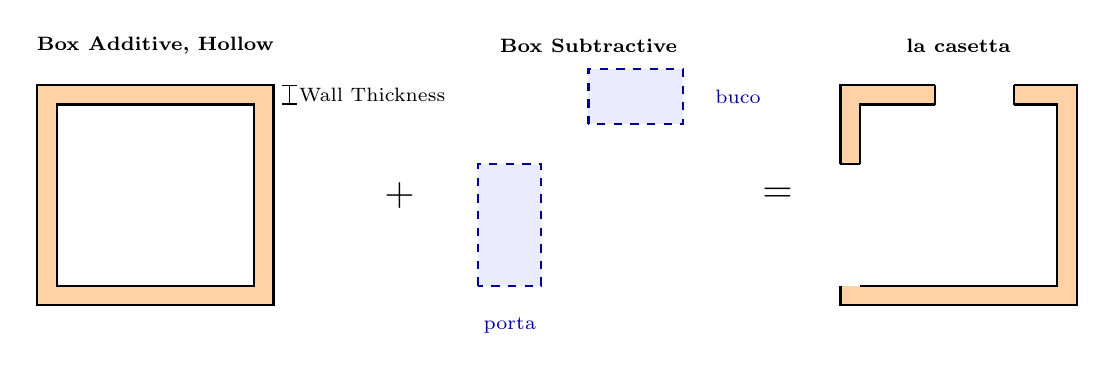
\begin{tikzpicture}[font=\footnotesize, x=1cm, y=1cm]
  % box additiva hollow (sezione)
  \node[font=\scriptsize\bfseries] at (1.5,3.3) {Box Additive, Hollow};
  \fill[orange!35] (0,0) rectangle (3,2.8);
  \fill[white] (0.25,0.25) rectangle (2.75,2.55);
  \draw[thick] (0,0) rectangle (3,2.8); \draw[thick] (0.25,0.25) rectangle (2.75,2.55);
  \draw[|-|, thin] (3.2,2.55) -- node[right, font=\scriptsize]{Wall Thickness} (3.2,2.8);
  \node at (4.6,1.4) {\Large $+$};
  % sottrattive
  \node[font=\scriptsize\bfseries] at (7.0,3.3) {Box Subtractive};
  \draw[thick, dashed, blue!60!black, fill=blue!8] (5.6,0.25) rectangle (6.4,1.8);
  \node[font=\scriptsize, blue!60!black] at (6.0,-0.25) {porta};
  \draw[thick, dashed, blue!60!black, fill=blue!8] (7.0,2.3) rectangle (8.2,3.0);
  \node[font=\scriptsize, blue!60!black] at (8.9,2.65) {buco};
  \node at (9.4,1.4) {\Large $=$};
  % risultato
  \begin{scope}[xshift=10.2cm]
    \node[font=\scriptsize\bfseries] at (1.5,3.3) {la casetta};
    \fill[orange!35] (0,0) rectangle (3,2.8);
    \fill[white] (0.25,0.25) rectangle (2.75,2.55);
    \fill[white] (-0.05,0.25) rectangle (0.3,1.8);
    \fill[white] (1.2,2.5) rectangle (2.2,2.85);
    \draw[thick] (0,1.8) -- (0,2.8) -- (1.2,2.8); \draw[thick] (2.2,2.8) -- (3,2.8) -- (3,0) -- (0,0) -- (0,0.25);
    \draw[thick] (0.25,1.8) -- (0.25,2.55) -- (1.2,2.55); \draw[thick] (2.2,2.55) -- (2.75,2.55) -- (2.75,0.25) -- (0.25,0.25);
    \draw[thick] (0,1.8) -- (0.25,1.8); \draw[thick] (1.2,2.55) -- (1.2,2.8); \draw[thick] (2.2,2.55) -- (2.2,2.8);
  \end{scope}
\end{tikzpicture}
\caption{Additive e Subtractive in sezione: una box additiva vuota (Hollow, con il suo
Wall Thickness) e due box sottrattive che la ``bucano'', una per la porta e una per il
buco sul soffitto da cui cadere nella stanza sottostante, come nella casetta costruita a
lezione. Ricostruzione schematica; le proporzioni sono indicative.}
\label{ue13:fig:csg}
\end{figure}

\paragraph{Il però: le brush sono pesanti.} ``Ora c'è un però, e il però è che le brush
sono \textbf{pesanti}.'' Se si riempie una scena di brush, ``perché volete diverse casette e
diverse zone dentro cui entrare'', ``si carica tanto sulla memoria del progetto''. Il
rimedio: \textbf{farla diventare una static mesh}. Nei Details della brush c'è il comando
per creare una static mesh dalla geometria (\emph{Create Static Mesh}, nella parte avanzata
dei Brush Settings), che chiede dove salvarla. Il docente lo fa con la casetta: nel
Content Browser compare ``un bloccone'', ma solo della brush selezionata (``se avessimo
selezionato tutte quante le brush, avremmo avuto un effetto diverso'': la mesh le avrebbe
comprese tutte). Il docente elimina la brush originale, ``non ci serve più'': la static mesh
che resta ``è molto meno pesante. Io posso riempirci la scena di questa roba qua.''
Bisognerebbe solo sistemarne il \textbf{pivot}, ``perché ce l'ho salvato col pivot
strano''. Un consiglio di ordine: invece di ``buttarla qui in mezzo al Content'', come ha
fatto lui, create ``una \emph{new folder} che chiamate, che ne so, \textbf{Blockout
Assets}'', e lì dentro mettete tutto quello che create. (Poi le elimina: a lui non servono.)

\paragraph{Approfondimento: perché le brush pesano, e Create Static Mesh.} Le geometry
brush sono la versione moderna della geometria \textbf{BSP} (\emph{binary space
partitioning}) delle vecchie versioni di Unreal: le brush additive e sottrattive vengono
combinate, nell'ordine in cui sono state create, in un'unica geometria del livello, che
l'editor ricalcola (\emph{Build Geometry}) quando le si modifica. Questa geometria non si
può istanziare, non ha LOD, ha UV e lightmap generate automaticamente e la sua collisione
è meno efficiente di quella di una mesh: per questo, oltre che per la memoria, Epic
raccomanda di usarle per il block out e di convertirle (o sostituirle) con static mesh
nel livello finale. Il comando \textbf{Create Static Mesh} salva la geometria delle brush
selezionate come asset \emph{Static Mesh}, con i materiali delle facce come slot; la
mesh nasce con il pivot all'origine del mondo o della prima brush, che si corregge con il
\emph{Modeling Mode} (strumento \emph{Pivot}) o riposizionandola. Nel libro di Romero e
Sewell le brush non compaiono: il libro costruisce i livelli con static mesh duplicate
(capitolo 9, il pavimento duplicato con Alt e trascinamento per raddoppiare l'area di
gioco). Quanto al modeling tool, il \emph{Modeling Mode} esisteva già come plugin
sperimentale nelle ultime versioni di Unreal~4, ma è con Unreal~5 che è diventato uno
strumento standard dell'editor: la frase del docente è vera nella sostanza. Funzionamento
generale dell'engine, salvo il riferimento al libro.

% ---------------------------------------------------------------------
\section{Le altre forme e il Brush Editing}
\label{ue13:sec:forme}

``Vediamo effettivamente cosa ci permettono di fare le altre brush.'' (La box sottrattiva il
docente se la tiene, ``almeno vediamo''.)

\paragraph{Cone.} Ha sempre le stesse impostazioni per le facce. Nei Brush Settings: un
valore \textbf{Z}, l'altezza; un \textbf{Outer Radius}; un \textbf{Inner Radius}, che non
si può modificare finché il cono non è \textbf{Hollow}: ``se io la rendo vuota'' si vede
com'è dentro, e si crea una struttura ``sulla base di quello che a me serve''. Il docente ci
mette dentro la box sottrattiva: ``una capannola mezza favola, una tenda''. Si può aumentare
il numero di lati (\textbf{Sides}): da 3, ``una piramide, anzi un D4'', fino a 500. A 500
``ha un po' stutterato, e non ci sarà mai un momento in cui ti servirà avere un cono così
preciso'', ma più facce lo rendono ``un po' più smussato''.

\paragraph{Cylinder.} ``Più o meno le stesse cose'': l'altezza, l'Outer Radius (``quanto è
largo effettivamente''), le facce come per il cono, Hollow o no, e il tipo, additivo o
sottrattivo.

\paragraph{Sphere.} Il \textbf{Radius}, ``quanto è ampia'', e la \textbf{Tessellation},
``quanti blocchi ha, quindi quanto è sferica''.

\paragraph{Linear Stair.} Tutto si basa sullo scalino, ``come anche le altre scale'': la
lunghezza del singolo scalino (\textbf{Step Length}), l'altezza (\textbf{Step Height}), la
larghezza (\textbf{Step Width}) e il numero di scalini (\textbf{Num Steps}): ``aumentando
gli scalini, aumenta l'altezza e aumenta la distanza''. Poi \textbf{Add to First Step},
``quanto in alto in più deve essere il primo scalino'': ``vedete, lui alza un tot''.

\paragraph{Curved Stair.} Altezza e larghezza dello scalino, e in più:
\begin{itemize}
  \item l'\textbf{Inner Radius}, il raggio del cerchio interno: ``se è molto largo, le
        scale vengono più arcuate'';
  \item l'\textbf{Angle of Curve}, ``quanto deve curvare la scala'': di default 90 gradi,
        ``però potreste fare anche 180, 270, anche 360 gradi'', se volete ``una singola
        chiocciola'';
  \item Num Steps e Add to First Step, ``esattamente allo stesso modo'';
  \item \textbf{Counter Clockwise}, per le scale ``che vanno nell'altra direzione''.
\end{itemize}
``Con tutte queste, poi potete andare a creare effettivamente delle static mesh.''

\paragraph{Spiral Stair.} ``Gli stessi parametri'': Inner Radius, Step Width, Step Height,
e in più lo spessore del singolo gradino (\textbf{Step Thickness}), ``perché è costruita
proprio a gradoni, ognuno di questi è un oggetto a sé stante, tutti attaccati l'uno con
l'altro''. C'è poi il numero di scalini \emph{per 360 gradi} (\textbf{Num Steps Per 360}):
``se voi dite che devono esserci 33 scalini per fare 360 gradi, poi dovete aggiungere
abbastanza scalini per arrivare a fare 360 gradi''; abbassandolo, con lo stesso numero
totale di scalini (``50, 60'') ne servono meno per fare un giro. Infine si può rendere
liscio il soffitto (\textbf{Sloped Ceiling}) o il pavimento (\textbf{Sloped Floor}), ``e
quindi avere una sorta di scivolo, una rampa'', e Counter Clockwise.

\paragraph{Il Brush Editing.} ``Prima facciamo un'ultima roba'': passare dalla
\textbf{Selection Mode} al \textbf{Brush Editing} (dal menu delle modalità dell'editor). Qui
si fanno ``piccole operazioni di modellazione'': selezionare un \textbf{vertice} e
spostarlo, una \textbf{faccia} e muoverla, un \textbf{edge} e muoverlo, ``in questo modo ci
andiamo a creare esattamente il tipo d'oggetto che serve a noi, anche se la forma che
serve a noi non c'era'' fra le brush. E lo \textbf{Split}: ``fa passare una serie di
vertici e di edge a tagliare'', una sezione dell'oggetto; ``si formano nuove facce, e
queste nuove facce possono essere prese e modificate''. ``Non so quanto spesso vi tornerà
utile fare un ecomostro del genere, però avete la possibilità di farlo.'' Un'avvertenza
emersa dalla prova: dopo le modifiche, l'oggetto ``è ancora una brush'', ma ``appena
l'andiamo a modificare'' dai Brush Settings ``ritorna come era precedentemente'': i
parametri ricostruiscono la forma da zero e cancellano le modifiche manuali.

\begin{table}[htbp]
\centering
\small
\begin{tabular}{@{}p{2.5cm}p{11.5cm}@{}}
\toprule
\textbf{Brush} & \textbf{Parametri (Brush Settings)} \\
\midrule
tutte & Brush Type: Additive / Subtractive; i materiali e le UV si impostano per faccia \\
Box & X, Y, Z; Wall Thickness (default 10); Hollow; Tessellated (solo se non hollow) \\
Cone & Z (altezza); Cap Z; Outer Radius; Inner Radius (solo se hollow); Sides (da 3 a
500); Align to Side; Hollow \\
Cylinder & Z; Outer Radius; Inner Radius (solo se hollow); Sides; Align to Side; Hollow \\
Sphere & Radius; Tessellation \\
Linear Stair & Step Length; Step Height; Step Width; Num Steps; Add to First Step \\
Curved Stair & Inner Radius; Step Height; Step Width; Angle of Curve (default
90$^\circ$); Num Steps; Add to First Step; Counter Clockwise \\
Spiral Stair & Inner Radius; Step Width; Step Height; Step Thickness; Num Steps Per 360;
Num Steps; Sloped Ceiling; Sloped Floor; Counter Clockwise \\
\bottomrule
\end{tabular}
\caption{Le geometry brush e i loro parametri. I nomi sono quelli dei Details di Unreal
Engine~5; quelli non letti a lezione (Cap Z, Align to Side) sono completati come
approfondimento.}
\label{ue13:tab:brush}
\end{table}

``Sono le cinque e mezza.'' Il docente annuncia che, al ritorno dalla pausa, si potrebbe
fare ``un piccolo block out utilizzando gli oggetti che avete'': le brush, le static mesh e
gli oggetti fatti con Igor, ``per cui magari vi piazzate dei collectible da raggiungere in
giro'', ``anche molto semplice''. Pausa di un quarto d'ora: ``facciamo 45''.

% ---------------------------------------------------------------------
\section{La pausa e la scelta del formato}
\label{ue13:sec:pausa}

(Durante la pausa la trascrizione contiene solo il blocco di testo ripetuto citato
nell'introduzione.) Alla ripresa c'è un problema di volume (``stavo leggendo il messaggio
che aveva scritto Augusto in chat'') e l'appello: Federico c'è, Guido ``c'è, ma non gli
funziona la telecamera'' (``basta che siete responsivi'').

\paragraph{La domanda del docente.} ``Ci stavo pensando adesso che stavamo fermi'': come
preferiscono strutturare le lezioni?
\begin{enumerate}
  \item una prima parte di spiegazione e una seconda in cui gli studenti ``provano a
        costruire qualcosa'', magari in streaming, ``così gli altri vedono anche cosa
        fate'' e il docente può commentare;
  \item tutte e tre le ore di spiegazione, con il lavoro pratico fra una lezione e l'altra
        e i feedback all'inizio della lezione successiva. Il tempo a disposizione cambia:
        ``da oggi, che è giovedì, fino a martedì avrete più tempo; da martedì a giovedì ne
        avrete meno''.
\end{enumerate}
Un primo studente preferisce la prima opzione, ``perché almeno abbiamo dei feedback diretti
e ci si può soffermare di più sulle varie cose''. Un altro la seconda, ``perché forse
riusciamo a fare più cose'', ``vediamo un po' più di argomenti''. Il docente avverte che le
cose che si faranno con lui ``sono tendenzialmente non troppo complesse, è più una
questione di metterle assieme'', e che non vorrebbe la situazione in cui ``io vi dico
facciamo questa cosa, la prossima volta me lo fate vedere e nessuno fa niente''. Edoardo,
alle prese con il caldo, dice che fare le cose fra una lezione e l'altra ``non è un peso''
se trova una soluzione; un altro: ``personalmente mi piace la seconda''. Il voto (``siete
dispari, quindi uscirà fuori una verità o l'altra''; ``per chi ci guarda da casa sarà tutto
in mano alle persone che erano qui'') premia la \textbf{seconda}: ``Tommaso, indipendentemente
dal tuo input, il popolo ha deciso di riempire la lezione con delle cose che magari faccio
io''.

Conseguenze: la lezione sullo \textbf{speed level design} andrà ``rimaneggiata'', ``perché
non so quanto ha senso che io mi metta a fare uno speed level per tre ore con voi che mi
guardate''; era ``una roba che mi sarebbe piaciuto far fare a voi''. Per la volta successiva,
a chi vuole, il docente chiede ``un piccolo livellino'' con geometrie e static mesh, ``per
giocare un po''': ``è molto bello sapere come funziona Unreal, però deve esserci del
\textbf{divertimento} nella creazione. Io mi devo divertire mentre creo il gioco.'' Le
indicazioni precise arrivano a fine lezione (sezione~\ref{ue13:sec:compiti}).

\paragraph{Che cosa fare nell'ora rimasta.} Personalizzare i parametri del bot in una gym
``è relativamente fine a se stesso'', ``un discorso abbastanza semplice'' che gli studenti
possono fare da soli. Meglio un altro actor interessante: le \textbf{luci}, e ``se riesco,
un accennino di post process''. Le luci si vedranno ``in un vuoto'', ``senza un dressing già
finito'', e si riprenderanno quando si parlerà di \emph{enrichment}, di dressing e di
ambienti, con lo speed level; per quella lezione il docente potrebbe preparare
``un ambientino'' o passare un pacchetto, ``così chi vuole lo fa assieme a me''. Le slide
non servono: ``faremo a braccio''. (Di nuovo problemi con Zoom: ``ogni volta che parto con la
stream non funziona il tasto destro''.) Il docente costruisce con una grande box un
ambientino chiuso (``così abbiamo un po' d'ombra''), invitando Filippo, che preferiva fare
le cose insieme, a sperimentare in parallelo. (Una parte della costruzione, nella
trascrizione, è incomprensibile: ``me la metà? E questa la facciamo? Giusto per fare
razzola''.)

% ---------------------------------------------------------------------
\section{Le luci: i tipi e la mobility}
\label{ue13:sec:mobility}

``Cos'è che non sta più funzionando in quella zona lì?'' Dentro la box: ``la luce del sole'',
risponde uno studente. La luce del sole è un tipo di luce, ``la signora
\textbf{Directional Light}''. Le luci di Unreal sono cinque: \textbf{Directional},
\textbf{Point}, \textbf{Spot}, \textbf{Rect} e \textbf{Sky Light}. Secondo la classificazione
del docente:
\begin{itemize}
  \item directional e sky light sono \textbf{luci ambientali};
  \item point e spot light si usano ``principalmente per l'illuminazione'';
  \item la rect light ``principalmente per i riflessi o per delle luci specifiche''.
\end{itemize}

\paragraph{Il costo dei rimbalzi.} ``Una cosa importante da dire è che il modo in cui Unreal
calcola le luci è simulando delle onde'' e il modo in cui ``queste onde luminose rimbalzano
sulle superfici''. Ci saranno situazioni in cui a una luce verranno chiesti ``troppi
rimbalzi, che equivalgono a troppi calcoli, che equivalgono a un peso molto elevato'':
bisogna stare attenti a come si posizionano le luci. (Sull'idea delle ``onde'' si veda
l'approfondimento alla fine della sezione.)

\paragraph{La Mobility.} ``Un parametro fondamentale che c'è in tutte le luci'' è la
\textbf{Mobility}: di default le luci sono \textbf{Stationary}, ma ci sono anche
\textbf{Static} e \textbf{Movable}. ``Non mi aspetto una risposta super completa, voglio
vedere se riusciamo ad arrivarci'' (``basta che ci passate sopra col mouse e ve lo dice
cosa fanno, però state con me''). Le ipotesi degli studenti: movable ``sarà tipo la luce di
una macchina''; stazionaria ``che sta ferma e non si muove'', ma statica ``mi sembra simile
come significato''; un altro propone ``statica un lampione, stazionaria il faro di una
macchina ferma, che potenzialmente si può muovere''; un altro ancora che la movable
``dovrebbe avere delle proprietà fisiche, magari condizionata dalla gravità'' (``la gravità
non c'entra''); un altro l'angolazione (``no, l'angolazione dipende dal tipo di luce che
utilizziamo''). Il docente rinuncia alla prova pratica (``qui c'è un po' di fregatura,
perché siamo in preview'') e parte dagli usi:
\begin{itemize}
  \item una luce \textbf{movable} è quella di ``una torcia a mano'', di una torcia
        elettrica che si punta, dei fari di una macchina, delle luci di un aereo: ``qualcosa
        in movimento'';
  \item una luce \textbf{stazionaria} è quella di un lampione, di un soffitto, ``di una
        qualsiasi luce di una casa'' \emph{dentro} il livello;
  \item una luce \textbf{statica} serve agli stessi scopi della stazionaria, ``ma fuori dal
        vostro livello''.
\end{itemize}
``Cosa cambia fra statica e stazionaria?'' Uno studente: ``nella stazionaria ci può
interagire un actor come il character''. ``Esatto.'' Le proprietà sono due: se si muove la
luce, l'ambiente reagisce?; se si passa davanti alla luce, la luce reagisce?
(figura~\ref{ue13:fig:mobility}):
\begin{itemize}
  \item la luce \textbf{statica} ``viene cucinata sulla scena'': è \emph{baked}
        completamente nell'editor e non si può modificare in gioco. Quando si
        \emph{buildano} le luci o si esporta il livello, ``la luce viene bakeata ed è
        impressa sulla scena''. Se si sposta l'actor della luce, la luce ``rimane dove è
        stata bakeata''; se il character ci passa davanti, la luce non reagisce. Si usa ``in
        tutti quei posti in cui so che non avrà interazioni e sarà soltanto luce
        d'atmosfera, luce d'ambiente''. È ``il tipo di luce più leggero'';
  \item la luce \textbf{stazionaria} ``se la muovo si rompe, ma se sta ferma e io ci passo
        davanti interagisce con me'': il character proietta ombre corrette, ma se si sposta
        la luce dopo il bake, la luce non si aggiorna;
  \item la luce \textbf{movable} ``fa entrambe le cose'': è completamente dinamica, reagisce
        agli oggetti e può essere spostata ``senza nessun problema''.
\end{itemize}

\begin{figure}[htbp]
\centering
\begin{tikzpicture}[font=\footnotesize, x=1cm, y=1cm,
  ue13col/.style={draw, thick, rounded corners=3pt, minimum width=4.0cm, minimum height=0.8cm,
                  align=center}]
  \node[ue13col, fill=gray!15] (st) at (0,0) {\textbf{Static}};
  \node[ue13col, fill=yellow!30] (sy) at (4.6,0) {\textbf{Stationary} (default)};
  \node[ue13col, fill=orange!30] (mv) at (9.2,0) {\textbf{Movable}};
  \node[align=left, anchor=north, text width=4.0cm] at (0,-0.6)
    {\textbf{bake}: sì, tutta\\ \textbf{si sposta in gioco}: no\\ \textbf{ombre dei personaggi}: no\\
     \textbf{costo}: il più basso\\[2pt] \emph{luce d'ambiente fuori dall'area di gioco}};
  \node[align=left, anchor=north, text width=4.0cm] at (4.6,-0.6)
    {\textbf{bake}: sì, la parte fissa\\ \textbf{si sposta in gioco}: no\\ \textbf{ombre dei personaggi}: sì\\
     \textbf{costo}: medio\\[2pt] \emph{lampioni, luci di casa, soffitti}};
  \node[align=left, anchor=north, text width=4.0cm] at (9.2,-0.6)
    {\textbf{bake}: no\\ \textbf{si sposta in gioco}: sì\\ \textbf{ombre dei personaggi}: sì\\
     \textbf{costo}: il più alto\\[2pt] \emph{torce, fari, luci di un aereo}};
  \draw[-{Stealth[length=2.5mm]}, very thick, gray] (-2.0,-3.3) -- node[below, font=\scriptsize]{più dinamica, più pesante} (11.2,-3.3);
\end{tikzpicture}
\caption{Le tre Mobility delle luci come le descrive il docente: che cosa viene
precalcolato (\emph{baked}), se la luce si può spostare in gioco, se reagisce ai personaggi
che le passano davanti, quanto pesa e per che cosa si usa.}
\label{ue13:fig:mobility}
\end{figure}

\paragraph{Approfondimento: onde, raggi e Lumen.} L'immagine delle ``onde'' è una
semplificazione del docente: Unreal non simula la luce come un'onda (niente interferenza o
diffrazione), ma come energia che viaggia in linea retta e rimbalza, cioè per
\emph{raggi}. Il calcolo dei rimbalzi (l'illuminazione \emph{globale}) avviene in due modi:
precalcolato, con \textbf{Lightmass}, che scrive il risultato nelle \emph{lightmap} delle
superfici al momento del build (luci static e stationary); o in tempo reale, con
\textbf{Lumen}, il sistema di illuminazione globale dinamica che Unreal Engine~5 attiva di
default nei progetti nuovi. Il principio del docente resta valido: più superfici e più
luci si sovrappongono, più calcoli servono, che siano fatti una volta nel build o a ogni
frame. Sulla stationary, un dettaglio in più: in gioco se ne possono cambiare colore e
intensità (non la posizione), e le ombre che proietta sugli oggetti fermi sono precalcolate,
mentre quelle degli oggetti in movimento sono dinamiche. Romero e Sewell (capitolo 4)
mettono la \emph{Mobility} di una point light a \textbf{Movable} proprio ``per poter
cambiare le proprietà della luce durante l'esecuzione'', quando la accendono e la spengono
da Blueprint. Funzionamento generale dell'engine, salvo il riferimento al libro.

% ---------------------------------------------------------------------
\section{La directional light e la sky light}
\label{ue13:sec:directional}

Il docente porta la directional light e la sky light ``tutte nello stesso posto''.
``Spostare queste luci non ha nessun tipo d'effetto.'' Perché?

\paragraph{La Directional Light.} Si può muoverla e scalarla ``come voglio e non cambia
assolutamente nulla. Ma se la ruoto, la luce reagisce.'' (``In questo caso reagisce anche''
un altro actor del cielo, ``perché è collegato'': la trascrizione dice ``la Schakespeare'' e
``la Schiapunsky'', con ogni probabilità la \emph{Sky Sphere} o la \emph{Sky Atmosphere}
del livello; il nome esatto non è ricostruibile.) La ragione: ``la directional light è
composta in una maniera abbastanza peculiare: è un \textbf{fascio di rette parallele} che
prende tutta la scena''. Spostarla non cambia nulla; ruotarla cambia ``il modo in cui viene
indirizzata la luminosità''. I parametri interessanti:
\begin{itemize}
  \item l'\textbf{Intensity}: aumentandola, ``va in questo caso a bruciare un pochino tutta la
        scena'' (``l'intensità della luce calcolata in X'': l'unità di misura nella
        trascrizione è incomprensibile; per la directional è il \emph{lux});
  \item il \textbf{Light Color}: una ruota dei colori per il colore della luce, la sua
        saturazione, ``quanto sarà scura, magari quanto sarà livida''. Se si vuole che più
        luci abbiano lo stesso colore, si copia il codice \textbf{Hex Linear} e lo si incolla
        nelle altre, ``il modo più comodo piuttosto che cercare a mano di replicare la stessa
        luce'': per esempio un corridoio in cui tutte le torce sono ``molto calde, molto
        accese, molto infuocate'';
  \item la \textbf{Temperature} (con \emph{Use Temperature}), per una luce ``tendenzialmente
        più calda o più fredda''; ``così, se volete fare \emph{Breaking Bad} quando sono in
        Messico, tutto giallo'';
  \item \textbf{Affects World}: ``questa luce che sto utilizzando ha effetto sul mondo? È una
        luce attiva o disabilitata?''. Serve, per esempio, a vedere ``come contribuisce alla
        scena'' una luce alla volta;
  \item \textbf{Cast Shadows}: la luce illumina comunque, ma proietta le ombre solo se è
        attivo;
  \item la \textbf{Dynamic Shadow Distance}: secondo il docente, ``quanto precisamente
        viene calcolata l'ombra, quanto è netta''. ``Non può essere notato adesso perché
        stiamo utilizzando solo geometrie''; con asset veri un valore basso si nota. Il
        docente cerca nel progetto una mappa già arredata per mostrarlo (``mi sa che non ne
        abbiamo, a parte quelle che ha fatto Igor'') e rimanda: ``la prossima volta mi
        preparo una scenetta carina a livello estetico''. È un parametro che ``tende ad
        appesantire un pochino le scene'', ma ``l'effetto che fa è talmente meglio rispetto a
        non averlo'': ``giocatevi un po' di potenza in più''.
\end{itemize}

\paragraph{Una sola per scena.} ``Non dovete mai avere \textbf{due directional} nella stessa
scena'': l'engine prova a calcolarle entrambe, ``fa molta fatica'' e ``il risultato è
tremendo'', con problemi di ombre calcolate in direzioni diverse. Allo stesso modo
``evitate di avere due sky sphere'', anzi, si corregge, due \textbf{sky light}: ``skylight e
directional light, una soltanto per scena''.

\paragraph{La Sky Light.} ``Funziona in maniera un po' diversa'', ``un po' più complessa'', e
``al momento non ci serve troppo indagarla''. Che cosa fa: ``è la luce che dà il
\textbf{mood}, la diffusione'', ``va a colorare l'aria, va a dare colore alla scena''. Si vede
cambiando il colore della sky light: cambiano di colore le \emph{ombre}. Per una scena al
tramonto, ``piuttosto che avere solo la directional che è arancione'', si media fra
directional e sky light, ``più tutta una serie di altre cose, perché utilizzeremo anche il
post process'' (la volta successiva). Fra i parametri, oltre all'intensità, quelli
dell'\textbf{ambient occlusion}: la distanza massima (\emph{Occlusion Max Distance}), il
contrasto (\emph{Contrast}) e ``quanto è moltiplicata'' (\emph{Occlusion Exponent} e
\emph{Min Occlusion}); e anche qui Cast Shadows e Affects World. ``Principalmente, mood
della scena e ambient occlusion.''

\paragraph{Approfondimento: Dynamic Shadow Distance, e due directional.} Il nome completo
del parametro è \emph{Dynamic Shadow Distance Movable Light} (o \emph{Stationary Light}, a
seconda della mobility): è la distanza dalla camera entro cui la directional disegna le
ombre dinamiche, divise in \emph{cascate} (\emph{Cascaded Shadow Maps}) di risoluzione
decrescente. Non è quindi la ``nettezza'' in sé, ma lo spazio su cui la risoluzione delle
ombre viene distribuita: oltre quella distanza le ombre dinamiche spariscono (restano solo
quelle precalcolate), e allungarla, a parità di cascate, rende le ombre vicine meno
dettagliate. In Unreal Engine~5, con le \emph{Virtual Shadow Maps} attive di default, questo
compromesso pesa molto meno. Sulle due directional, la regola del docente è la pratica
comune; a rigore Unreal ne supporta due solo come sole e luna dell'atmosfera (indice
\emph{Atmosphere Sun Light Index} 0 e 1), un caso particolare. Funzionamento generale
dell'engine.

% ---------------------------------------------------------------------
\section{Point light e spot light}
\label{ue13:sec:point}

``Passando a delle luci con cui andrete a smanettare molto ma molto di più'': le luci
``antropiche'', quelle che si useranno ``per fare quasi tutto'', \textbf{point light} e
\textbf{spot light}. ``Fra le due, qual è più leggera, più facile da calcolare,
indipendentemente dalla mobility?''

\paragraph{La domanda.} Uno studente risponde la point light, ``perché non si va a calcolare
anche la direzione''. ``È esattamente il contrario.'' La point light è a 360 gradi: ``lui
calcola contemporaneamente tutte le direzioni''. La \textbf{spot light} è più leggera
``perché non va a calcolare i rimbalzi della luce nelle altre direzioni'': ``la discriminante
è quella della direzione''. In una scena affollata, la spot illumina solo dove la si punta,
mentre la point ``va posizionata con attenzione perché va a colpire anche gli oggetti che ha
alle spalle'', ``indiscriminatamente dalla direzione''.

\paragraph{L'Attenuation Radius.} Per la point light, ``i due parametri più importanti sono
l'intensità e l'\textbf{Attenuation Radius}'', la sfera che si vede attorno alla luce.
``Indipendentemente dal fatto che io ho messo 10.000 miliardi di intensità, se il raggio non
tocca nulla la luce non illumina'' (o meglio, illumina solo dentro la sfera, ``quindi non
rimbalza su niente''). È ``il raggio massimo entro cui la luce avrà effetto'', e gestisce
un'attenuazione dalla sorgente fino al bordo: il \emph{gradiente} della luce. Con
un'intensità altissima, per un'attenuazione sensata bisogna ingrandire molto il raggio. Ma
anche con un'intensità bassa l'attenuazione arriva fino al bordo, e questo è il punto: il
raggio è ``il parametro che va gestito con attenzione'', ``perché determina con quanti
oggetti la luce andrà a compenetrare'', e quindi quante ombre dovrà proiettare. ``Anche se
l'intensità è molto bassa, nel momento in cui questo muro è all'interno del raggio,
l'engine dovrà calcolare'' l'ombra e la luce su quella superficie.

\paragraph{La X rossa.} ``Una cosa che vi capiterà sicuramente'': una luce con una
\textbf{X rossa} sopra. Il docente la riproduce mettendo più luci vicine (al primo tentativo
``non abbastanza'': i raggi erano piccoli). Vuol dire che ``l'engine ha rinunciato a far
proiettare ombre a questa luce'': la luce illumina comunque, ``ma non proietta ombre perché
ci sono troppe altre luci con cui questa luce sta compenetrando''. L'engine lo segnala come
problema, ``non grave''. I rimedi sono due: dire noi alla luce di non proiettare ombre
(Cast Shadows disattivato), così l'engine ``non cercherà costantemente di proiettarle'';
oppure \textbf{ridurre il raggio} ``a tal punto da non farlo compenetrare con troppe cose''.
``Non riempite la vostra scena di luci, piuttosto utilizzate \textbf{poche luci molto
significative}.''

\paragraph{Il corridoio.} L'esempio: un corridoio con una fila di luci. Mentre il
personaggio passa, le ombre sono corrette ``fino a che non arriviamo qui vicino'': lì la
luce viene calcolata ``come se questa non ci fosse'', e l'ombra viene proiettata dalle due
luci ai lati. ``Vedete, qui skippa, qui salta'': l'ombra della luce con la X non c'è, c'è
solo quella della luce ``un po' più lontana'', mentre altrove l'ombra è ``molto più forte,
molto più precisa, molto più netta''. ``Se replicate questo esperimento per conto vostro, vi
rendete conto che è abbastanza semplice da replicare.''

\paragraph{La sorgente: Source Radius, Soft Source Radius, Source Length.} Come illuminare
un corridoio ``piuttosto che avere una luce per torcia, una luce per punto''? Si modifica la
\textbf{sorgente}: ingrandendo il \textbf{Source Radius} e allungando la \textbf{Source
Length}, la luce non parte più da un punto ma ``da un cilindro, da una capsula'', ed è
``più distribuita''. Il raggio può anche essere zero, ``se volete una linea e basta''. È
così che si fanno illuminazioni particolari, ``tipo un locale illuminato unicamente dalla
luce dei \textbf{neon}'': mesh con materiali \textbf{emissive}, ``che quindi già emettono una
piccola luce di loro'', più luci distribuite ``in maniera più omogenea'' in questo modo. Il
\textbf{Soft Source Radius} ``serve per creare un'altra lucina interna, come quando puntate
una torcia verso il muro'': una parte più attenuata all'esterno e una meno attenuata
all'interno (``si vede meglio con la spot''; il docente non riesce a mostrarlo bene). Più
sotto ci sono di nuovo Affects World e Cast Shadows, e lo \emph{scattering} con la nebbia
volumetrica (\emph{Volumetric Scattering Intensity}), che servirà quando si userà una
nebbia (la trascrizione dice ``una FOD'', con ogni probabilità \emph{fog}); poi ``molti, molti
parametri'' per le ombre (risoluzione, comportamento sulle pendenze). ``Non tutti vi
servono'', ``a meno che non vogliate fare proprio il \emph{light artist}''. (``Non l'ho
detto prima'': anche la point light ha il Light Color, ``per fare le vostre luci da inferno,
da nightclub, da \emph{Night City}''.)

\paragraph{La spot light.} È fatta a \textbf{cono}, quindi si ruota. Intensità e Light
Color come le altre; l'\textbf{Attenuation Radius}, qui, ``non dipende da quanto è la
sfera, ma è la lunghezza del cono'', ``quanto in là viene proiettata'': ``se sta così non
colpisce il muro, così illumina questa parte del muro''. Poi due angoli
(figura~\ref{ue13:fig:luci}):
\begin{itemize}
  \item l'\textbf{Outer Cone Angle}, che gestisce il cono;
  \item l'\textbf{Inner Cone Angle}, il cono interno, ``l'effetto torcia'': nella parte
        colpita dall'inner cone ``ci sarà una minore attenuazione''. Con i due angoli vicini
        il bordo è netto; ``volendo potete avere anche un cono che non attenua mai alla
        base, che attenua soltanto sulla distanza''. Questo cono serve a determinare la
        \emph{sfumatura}, ``ed è anche quello che faceva l'altro nella point, ma con questo
        si nota meglio''.
\end{itemize}
Anche qui Source Radius, Source Length e Soft Source Radius, e i parametri delle ombre.

\paragraph{La domanda sull'effetto accecante.} Uno studente chiede se, guardando
direttamente la luce, ci sia ``l'effetto accecante''. ``No, assolutamente no.'' L'effetto
``tipo quando guardi il sole'' si crea con il \textbf{post process}, che il docente vuole
far vedere ``quando abbiamo una mappa che non sia soltanto delle geometrie'' (con un
pacchetto di mesh e mappe già fatte: ``sono abbastanza sicuro che questo pacchetto dovesse
avere delle mappe''). Con i parametri del post process si aggiungono \textbf{bloom} e
\textbf{lens flare}. Altro esempio: i \textbf{god rays} (``god shaft''), ``una luce molto
forte che entra dalla finestra e c'è questa proiezione luminosa che taglia la scena''.
``Quella roba lì con la luce non puoi farla. Ti serve la luce, ma devi andare a manipolare
il modo in cui la telecamera vede la luce con la post produzione.'' Per questo ``la post
produzione va fatta dopo le luci'': ``prende l'illuminazione della scena e ci aggiunge delle
lenti, degli effetti''. Fra le ``lenti'', oltre al bloom: la messa a fuoco, la distorsione,
la \emph{chromatic aberration}.

\begin{figure}[htbp]
\centering
\begin{tikzpicture}[font=\footnotesize, x=1cm, y=1cm]
  % point light
  \node[font=\scriptsize\bfseries] at (1.6,3.4) {Point Light};
  \shade[inner color=yellow!70, outer color=white] (1.6,1.6) circle (1.5);
  \draw[dashed, thick, orange!70!black] (1.6,1.6) circle (1.5);
  \fill[orange] (1.6,1.6) circle (0.08);
  \draw[-{Stealth[length=1.6mm]}] (1.6,1.6) -- (2.66,2.66);
  \node[font=\scriptsize, align=center] at (1.6,-0.5) {Attenuation Radius = sfera;\\360$^\circ$: colpisce anche\\ciò che ha alle spalle};
  % spot light
  \begin{scope}[xshift=4.4cm]
    \node[font=\scriptsize\bfseries] at (1.6,3.4) {Spot Light};
    \fill[yellow!25] (0.2,2.8) -- (3.2,0.2) -- (0.9,0.0) -- cycle;
    \fill[yellow!65] (0.2,2.8) -- (2.55,0.4) -- (1.55,0.1) -- cycle;
    \draw[dashed, thick, orange!70!black] (0.2,2.8) -- (3.2,0.2);
    \draw[dashed, thick, orange!70!black] (0.2,2.8) -- (0.9,0.0);
    \fill[orange] (0.2,2.8) circle (0.08);
    \node[font=\scriptsize, anchor=west] at (2.7,1.3) {Outer Cone};
    \node[font=\scriptsize, anchor=west, fill=white, inner sep=1pt] at (1.25,1.15) {Inner};
    \node[font=\scriptsize, align=center] at (1.6,-0.5) {Attenuation Radius =\\lunghezza del cono};
  \end{scope}
  % rect light
  \begin{scope}[xshift=8.8cm]
    \node[font=\scriptsize\bfseries] at (1.8,3.4) {Rect Light};
    \fill[yellow!30] (0.9,2.4) -- (2.7,2.4) -- (3.4,0.2) -- (0.2,0.2) -- cycle;
    \draw[very thick, fill=orange!60] (0.9,2.4) rectangle (2.7,2.6);
    \draw[very thick, gray!70!black] (0.9,2.4) -- (0.55,1.95);
    \draw[very thick, gray!70!black] (2.7,2.4) -- (3.05,1.95);
    \node[font=\scriptsize, anchor=east] at (0.55,2.0) {Barn Door};
    \node[font=\scriptsize, align=center] at (1.8,-0.5) {Source Width $\times$ Height;\\Barn Door Angle e Length};
  \end{scope}
\end{tikzpicture}
\caption{Le tre luci locali e i parametri che ne determinano la forma: la sfera di
attenuazione della point light, i due coni della spot light (nel cono interno
l'attenuazione è minore) e la sorgente rettangolare della rect light, con le ``porte da
stalla'' che ne restringono il fascio. Schema indicativo, non in scala.}
\label{ue13:fig:luci}
\end{figure}

\paragraph{Approfondimento: la X rossa, il costo delle ombre e i god rays.} La X rossa ha
una causa precisa: è il limite delle luci \textbf{stationary} sovrapposte. Le ombre
precalcolate delle stationary vengono scritte in quattro canali di una texture, quindi in
un punto qualsiasi del livello possono sovrapporsi al massimo \textbf{quattro} luci
stationary con le ombre attive (la directional conta come una); la quinta, segnata con la X
rossa, ripiega sulle ombre interamente dinamiche, più costose, o le perde (l'editor la
elenca nel \emph{Map Check}). Per questo i rimedi del docente funzionano: ridurre
l'Attenuation Radius toglie la sovrapposizione; disattivare Cast Shadows toglie la luce dal
conteggio; un'altra via è rendere la luce static o movable. Sul costo: la ragione per cui
una spot light è più economica di una point light sta soprattutto nelle ombre, perché una
spot proietta le ombre con una sola \emph{shadow map} orientata, mentre una point light ne
ha bisogno in tutte le direzioni (una \emph{cube map} di sei facce). Sui \textbf{god rays},
la frase del docente va presa nel suo senso: in Unreal l'effetto si ottiene con le opzioni
\emph{Light Shaft Occlusion} e \emph{Light Shaft Bloom} della directional light, o con la
\emph{Exponential Height Fog} con la nebbia volumetrica attiva; i light shaft sono
comunque un effetto calcolato sull'immagine della camera, quindi della stessa natura del
post process, come dice il docente. L'abbagliamento guardando il sole viene dal
\textbf{bloom} e dall'\textbf{esposizione automatica} (\emph{Eye Adaptation}), entrambi
impostati in un \textbf{Post Process Volume}. Romero e Sewell (capitolo 9) ricordano che il
\emph{Post Process Volume} e il \emph{Lightmass Importance Volume} del livello ``vanno
scalati per coprire l'area di gioco'' quando la si allarga, ``perché servono per
l'illuminazione e gli effetti''; e nel capitolo 12 che la qualità del post processing
(``motion blur e bloom'') e delle ombre (``i dettagli delle ombre hanno spesso un impatto
drammatico sulle prestazioni'') è fra le impostazioni di \emph{Engine Scalability}.
Funzionamento generale dell'engine, salvo i riferimenti al libro.

% ---------------------------------------------------------------------
\section{La rect light}
\label{ue13:sec:rect}

``Ora mi sono scordato le rect light.'' ``Sono un po' strane'': sembrano ``una spotlight,
ma tipo rettangolare'', e invece sono diverse. Si usano principalmente per le
\textbf{illuminazioni industriali}, ``le classiche luci quadrate da fabbrica'', o ``molto
più spesso'' per i \textbf{riflessi}: ``il riflesso della televisione su un pavimento''.
Vanno usate ``soltanto su oggetti rettangolari'' che proiettano una luce specifica, ``come
un'insegna al neon, di quelle dei locali''. ``Se devo farmi calcolare dei riflessi, lo
faccio utilizzando la rect light perché dà dei risultati più precisi.''

I parametri ``non sono troppo diversi'': intensità, colore, Attenuation Radius ``che ormai
abbiamo imparato a conoscere'', la larghezza e l'altezza della sorgente (\emph{Source Width},
\emph{Source Height}). Ciò che cambia:
\begin{itemize}
  \item il \textbf{Barn Door Angle}: la sorgente è un rettangolo centrale ``più una
        struttura lungo il rettangolo'', che Unreal chiama \emph{barn door} (``come si
        traduce?'', chiede il docente; ``la stalla'', risponde uno studente: le alette dei
        proiettori da set, dette appunto \emph{porte da stalla}). Cambiando l'angolo è
        ``come se ci fosse un'ostruzione'': le alette si piegano e la luce va solo in avanti;
        al massimo, la luce arriva fino a terra; nel mezzo, un effetto sfumato;
  \item la \textbf{Barn Door Length}, ``quanto è grande questa lente'', per ``un effetto tipo
        i riflettori degli stadi'', che illuminano ``una parte specifica, molto tagliata,
        molto netta'';
  \item la \textbf{Source Texture}: ``la texture che noi andiamo a inserire diventa il tipo di
        luce che viene messo'', come un'insegna o un televisore che proietta una luce
        particolare; ``è come se andasse a proiettare la luce attraverso un filtro, per
        spiegarlo in modo brutto''. Il docente cerca una texture riconoscibile nel progetto
        (``queste non vanno bene'') senza trovarla, e l'esempio resta a parole;
  \item anche qui la Temperature e Affects World.
\end{itemize}

% ---------------------------------------------------------------------
\section{Il build delle luci e i riflessi}
\label{ue13:sec:build}

``Stavo per scordare una delle parti fondamentali.'' La differenza fra static, stationary e
movable si vedeva ``molto meglio sulla quarta edizione''; ma anche sulla quinta ``dovete
stare attenti'': ``vi capiterà di fare dei livelli in cui avete un'illuminazione, poi andate
a buildare e la luce che vi ritrovate alla fine non è la luce che pensavate di avere''.
Questo perché le luci \textbf{statiche e stazionarie} hanno bisogno di essere
\textbf{buildate}.

\paragraph{La qualità del build.} Quando si fa il build bisogna scegliere la qualità con cui
calcolare le luci (\emph{Lighting Quality}): di default è \textbf{Preview}, ``la qualità
più veloce'', in cui ``vengono calcolati meno rimbalzi''; quando si pubblica un gioco si usa
\textbf{Production}, il livello più alto, che viene calcolato al build e ``rimane bakeato
sul livello''. Se non si fa il build, le luci statiche e stazionarie ``rimangono delle
preview''.

\paragraph{La ``bestemmia''.} ``Oppure utilizzate questa cosa che sto per dire, sarà una
bestemmia: utilizzate \textbf{solo luci movable}.'' Le movable sono pesanti, ``quindi non
utilizzate solo luci movable, chiaramente''; ma per un livello \emph{molto piccolo}, ``in cui
avete 2--3 luci massimo'', e che serve in fretta, avere luci movable ``che sono esattamente
come le vedete alla fine'' può tornare comodo. ``Se dovete illuminare un livello con 20 e
passa luci, non mettete solo luci movable'': mettete luci static e stationary e fate il
build.

\paragraph{Il menu Build.} Si possono buildare diverse cose, ``pezzo per pezzo'': le luci,
le \textbf{reflection capture} (``ecco che mi mancava, i riflessi''), la visibilità statica
(\emph{Precompute Static Visibility}), il \textbf{landscape} (``che poi vedremo la prossima
volta''), e così via; \textbf{Build All Levels} ribuilda tutto. ``Con la quinta edizione,
tutto sommato, ve la cavate'': in Unreal~4, senza il build, ci sarebbero scritte
\textbf{Preview} sparse per la scena e in alto \textbf{Lighting needs to be rebuilt}.
``Se mai vi capita di lavorare su una versione precedente di Unreal, sappiate che quella
scritta in alto è perché non avete buildato le luci''. In ogni caso: ``quando avete finito
il livello fate sempre un build generale''.

\paragraph{Le Reflection Capture.} I riflessi ``sono abbastanza scollegati
dall'illuminazione, ma funzionano in maniera simile'': anche loro sono \textbf{volumi} che
influenzano zone specifiche e vanno buildati. Si trovano fra i volumi: \textbf{Box
Reflection Capture}, \textbf{Planar Reflection} e \textbf{Sphere Reflection Capture}.
Prendendo la sfera, ``semplice da vedere'': ha un raggio di influenza (di default 3000), che
si ingrandisce e si riduce, e vi si possono assegnare mappe specifiche. Quando si fa il
build, ``catturano tutto quello che c'è all'interno della sfera e calcolano i riflessi sulle
superfici riflettenti''.

\paragraph{Quali superfici riflettono?} ``Perché anche se io buildo qui adesso lui non mi
farà vedere niente di diverso?'' Il docente rimanda alla lezione sui materiali: uno studente
ricorda i parametri ``quanto rifletto la luce, l'opacità''. ``Esatto'': i parametri che
contano sono \textbf{Metallic}, \textbf{Specular} e \textbf{Roughness}, ``soprattutto
Specular e Roughness'', che determinano quanto il materiale sarà riflettente. I materiali
della scena di prova non lo sono; con una roughness ``particolarmente bassa'' e una specular
``particolarmente alta'', tutti gli oggetti nell'area di cattura verrebbero riflessi sulle
superfici capaci di rifletterli: ``le pozzanghere, i pavimenti lucidi, gli specchi''. ``Magari
ci ritorniamo nel momento in cui abbiamo un ambiente più costruito, che non sia solo
blocchi.''

\paragraph{Approfondimento: il build in Unreal Engine 5.} Il motivo per cui ``con la quinta
ve la cavate'' è \textbf{Lumen}: nei progetti nuovi di Unreal Engine~5 l'illuminazione
globale e i riflessi sono calcolati in tempo reale, e una scena illuminata da luci movable
(o da stationary e static non ancora buildate) appare già come apparirà in gioco; i livelli
dei template, inoltre, partono spesso senza illuminazione precalcolata. Il build con
Lightmass serve quando si sceglie l'illuminazione precalcolata, di solito per ragioni di
prestazioni (piattaforme mobili, VR, scene molto statiche), e in quel caso valgono tutte le
avvertenze del docente: il build a qualità Production prima di pubblicare, il
\emph{Lightmass Importance Volume} attorno all'area di gioco, e il controllo del messaggio
``Lighting needs to be rebuilt'' (in Unreal~5 segnalato in modo meno vistoso). Anche le
\emph{Reflection Capture} perdono importanza con i riflessi di Lumen, ma restano il
ripiego quando Lumen è disattivato. La Sphere Reflection Capture ha di default un
\emph{Influence Radius} di 3000 unità (30 metri), il valore letto a lezione. Funzionamento
generale dell'engine; il libro di Romero e Sewell non tratta il build delle luci.

% ---------------------------------------------------------------------
\section{I compiti per martedì e la chiusura}
\label{ue13:sec:compiti}

``Abbiamo una decina di minuti.'' Le luci, ``accennate al volissimo'', si rivedranno con il
post process e con lo speed level, ``se riesco a farvi vedere qualcosina, almeno di che
cos'è concettualmente''. Uno studente chiede delle \emph{linee guida} per il lavoro della
volta successiva: ``delle specie di linee guida''. ``Molto fumose, molto generiche, però così
per darvi qualcosina'':
\begin{enumerate}
  \item una \textbf{gym} in cui si sono calcolati i parametri del proprio personaggio ``che
        ritenete importanti per il gameplay''. La Max Sprint Distance da 26 m serve solo se
        nel gioco ci sono cose a tempo: ``se voi volete fare soltanto un platform, magari
        questa cosa non vi serve''. Pensate ``a seconda del tipo di block out che volete
        fare'' e misurate quanto in alto salta, quanto velocemente si muove, quanto lontano
        salta, le differenze fra lo sprint e il salto, magari con una gravità modificata;
        le misure vanno tenute ``da una parte, all'interno del livello in cui andrete a fare
        il block out'';
  \item \textbf{smanettare con i parametri del bot}, BP\_Bot2, ``in modo da avere un tipo di
        esperienza che magari funziona meglio per il vostro gioco''. Esempio in diretta: il
        \textbf{Walkable Floor Angle}, ``44'' di default. Il docente fa delle rampe di
        pendenze diverse: su alcune il bot sale, su una più ripida ``lo fa scivolare giù''.
        Così si possono fare ``delle parti in cui il vostro robot non può andare, che non
        sono semplicemente dei muri''. O una gravità ``meno lunare''; o una camminata più
        veloce: ``io trovo che la camminata di base del robot, per i miei gusti, sia un po'
        lenta, quindi magari l'andrei a modificare''. E, ``una cosa carina'', il
        \textbf{margine di manovra e di errore}: il bot ``salta e non si muove a mezz'aria,
        ha un pessimo controllo a mezz'aria''; con l'\textbf{Air Control} a 1 ``si muove come
        se non fosse in aria''. ``Quanta libertà di movimento voglio dare al mio giocatore? Per
        quale motivo?'' La gym serve anche a rispondere a domande come: ``so che il mio
        personaggio salta 4 metri in avanti e 2 in alto: posso fare questo salto? E se posso
        farlo, è comodo farlo?'';
  \item un \textbf{piccolo block out} in cui l'obiettivo è prendere da \textbf{tre a cinque
        collezionabili}, ``ognuno ottenuto in una maniera diversa'': esplorando,
        saltellando, usando gli oggetti delle lezioni precedenti, ``schivando i colpi della
        mitraglietta'', ``quello che volete''. Serve a familiarizzare ``con l'idea di fare delle
        piccole sfide che il giocatore deve superare per raggiungere degli obiettivi''.
\end{enumerate}
Alla lezione successiva il docente chiederà che cosa è stato modificato e perché: ``poi
magari ci facciamo una chiacchiera sul perché avete deciso di dare quel tipo di parametro
al robottino e cosa volevate farci, che è l'inizio del design: iniziare a pensare a questi
numeri, in che modo influenzano l'esperienza del giocatore''.

Per chi ha problemi di surriscaldamento: ``provateci'', ``stiamo lavorando principalmente con
dei blocchi'', ``non c'è nulla di pesante da un punto di vista grafico''; ``le cose pesanti
verranno più avanti, quando cominceremo a utilizzare elementi estetici''. ``Penso di essermi
mangiato le mie parole tipo infinite volte, però di averle dette talmente tante volte che
era chiaro il concetto.'' Nessuna domanda. ``Ci becchiamo martedì prossimo'': per qualsiasi
cosa, il \textbf{Discord}, anche per mostrare il proprio lavoro.

\paragraph{Approfondimento: il compito visto dai libri.} Il compito mette insieme i temi
della giornata nell'ordine in cui Totten li presenta: prima le metriche (la gym), poi il
whiteblocking (il block out), poi le sfide costruite sulle metriche e sulle abilità del
personaggio. Due criteri dal suo capitolo 2 sono utili come controllo: ogni sfida dovrebbe
usare una metrica misurata (un salto vicino al limite, una distanza vicina alla Max Sprint
Distance, una pendenza oltre il Walkable Floor Angle) e dovrebbe essere \emph{leggibile},
cioè comunicare al primo sguardo se e come si supera, come il blocco da 1,40 m della
lezione. Romero e Sewell (capitolo 13) mostrano come trovare e piazzare rapidamente
actor di supporto dal \emph{Place Actors Panel} (lo stesso pannello usato a lezione per le
brush), comodo per disseminare il livello di collezionabili e punti di riferimento.

% ---------------------------------------------------------------------
\begin{table}[htbp]
\centering
\small
\begin{tabular}{@{}p{4.6cm}p{3.2cm}p{6.2cm}@{}}
\toprule
\textbf{Misura o valore} & \textbf{Valore} & \textbf{Dove e a che serve} \\
\midrule
Max Sprint Distance & 26 m & la corsa con una barra di stamina; limite per inseguimenti e
distanze fra ricariche \\
Margine sullo sprint & circa 20 m & dove mettere una ricarica di stamina \\
Walk Jump / Sprint Jump & 4 m / 6 m & la lunghezza dei salti del bot con Jump Z Velocity
modificata \\
Limiti per i salti di un platform & circa 2,20--2,30 m in alto, 5,80 m in lungo & le sfide
del livello, sotto i massimi \\
Blocchi d'altezza & 1; 1,40; 1,60; 1,80; 2 m & il feeling del salto; 1 m superato
``male'', 1,40 m no \\
Max Step Height & 45 cm (provato con 40 cm e 1 m) & il gradino che si sale camminando \\
Walkable Floor Angle & ``44'' (44,77$^\circ$) & la pendenza oltre cui il bot scivola \\
Jump Z Velocity & 420 $\to$ 700 (poi 600--650) & l'altezza del salto: con 700 oltre i 2 m \\
Air Control & fino a 1 & il controllo in aria (1 = come a terra) \\
Porte nella slide della gym & 4$\times$4, 2$\times$4, 2$\times$3, 2$\times$2,5,
2$\times$2 m & l'esperienza di passarci, con la camera in terza persona \\
Max comfortable wall run & 12 m (discesa da 13--14 m) & la slide della gym \\
Griglia del pavimento & 1 m, quadratini da 20 cm & leggere le misure; snapping a 10 cm \\
Box di prova & 600; Wall Thickness 10 $\to$ 50 & la casetta con le brush \\
Sides del Cone & da 3 a 500 & la precisione del cono \\
Sphere Reflection Capture & raggio 3000 & la zona di cattura dei riflessi \\
\bottomrule
\end{tabular}
\caption{Le misure e i valori della giornata. I valori del salto e della corsa sono quelli
trovati in diretta dal docente, che li definisce ``molto non calcolati'': il compito è
trovare i propri.}
\label{ue13:tab:misure}
\end{table}

\begin{table}[htbp]
\centering
\small
\begin{tabular}{@{}p{5.4cm}p{8.6cm}@{}}
\toprule
\textbf{Sintomo} & \textbf{Causa e rimedio} \\
\midrule
Il bot supera il blocco da 1 m ``scivolando'' & la capsula sale sullo spigolo: ostacolo
poco leggibile; alzarlo (1,40 m è chiaramente insuperabile) o renderlo chiaramente
superabile \\
Il bot sale su un ostacolo da 40 cm senza saltare & è sotto la Max Step Height (45 cm):
abbassarla se non va bene \\
Max Step Height a 1 m non fa salire il bot & salvare e compilare; poi restano i limiti della
capsula e degli altri parametri (non risolto a lezione) \\
Cambiare la Jump Z Velocity non ha effetto & si sta modificando il Blueprint sbagliato: il
personaggio in gioco è BP\_Bot2 \\
Il materiale della brush si deforma & la brush è stata scalata: usare X, Y, Z dei Brush
Settings \\
Il materiale va su una faccia sola & le brush hanno un materiale per faccia: assegnarlo a
ogni faccia \\
Inner Radius non modificabile & il cono (o il cilindro) non è Hollow \\
Tessellated non ha effetto & la box è Hollow \\
Le modifiche del Brush Editing spariscono & si è cambiato un parametro dei Brush Settings,
che ricostruisce la forma \\
La scena con molte brush è pesante & Create Static Mesh, poi eliminare la brush; mettere le
mesh in una cartella Blockout Assets; sistemare il pivot \\
Spostare la directional non cambia nulla & è un fascio di rette parallele: va ruotata \\
Ombre sbagliate con due directional (o due sky light) & una sola per scena \\
Una luce illumina poco nonostante l'intensità & l'Attenuation Radius non raggiunge le
superfici \\
X rossa su una luce, niente ombre & troppe luci (stationary) sovrapposte: ridurre il raggio
o disattivare Cast Shadows \\
Nel corridoio l'ombra ``salta'' & la luce con la X non proietta ombre: come sopra; o una sola
luce allungata (Source Length) \\
La luce finale non è quella vista nell'editor & luci static e stationary non buildate:
Build, qualità Production \\
Scritte Preview e ``Lighting needs to be rebuilt'' (Unreal 4) & build delle luci mancante \\
Le Reflection Capture non mostrano nulla & i materiali non sono riflettenti: Roughness bassa,
Specular alta \\
Il tasto destro non funziona durante la condivisione & problema di Zoom, non risolto \\
\bottomrule
\end{tabular}
\caption{I problemi incontrati durante la lezione, con la causa e il rimedio.}
\label{ue13:tab:errori}
\end{table}

\begin{table}[htbp]
\centering
\footnotesize
\begin{tabular}{@{}p{5.8cm}p{8.2cm}@{}}
\toprule
\textbf{Strumento, actor o impostazione} & \textbf{Che cosa fa} \\
\midrule
Level design document & descrive il livello in modo chiaro, né generico né costrittivo \\
Layout (piantina) & la mappa 2D del livello, con legenda; si sbaglia senza costi \\
Gym (test level) & il livello in cui si misurano le metriche del personaggio \\
Block out & il livello rifatto con sole geometrie, per testare il gameplay \\
Landmark & oggetto riconoscibile che dà identità e orienta \\
Snapping della griglia & sposta gli actor a passi fissi (10 cm) \\
Text Render (approfondimento) & testo nel livello, per i cartelli delle misure \\
Character Movement & il componente dei parametri di movimento del personaggio \\
Quick Add (menu), voce Geometry & aggiunge le brush e gli altri actor \\
Place Actors Panel & pannello agganciabile con tutti gli actor da piazzare \\
Geometry Brush: Box, Cone, Cylinder, Sphere, Linear, Curved e Spiral Stair & le forme di
base per il block out \\
Brush Type: Additive / Subtractive & aggiunge geometria; la toglie (buchi, porte, finestre) \\
Hollow, Wall Thickness, Tessellated & vuota; spessore dei muri; divisa in triangoli \\
Create Static Mesh (Brush Settings) & salva la brush come static mesh, più leggera \\
Brush Editing (modalità) & sposta vertici, edge e facce; Split per tagliare \\
Directional Light & il sole: rette parallele, conta solo la rotazione \\
Sky Light & il colore dell'ambiente, il mood, l'ambient occlusion \\
Point Light / Spot Light / Rect Light & luce in tutte le direzioni; a cono; da una sorgente
rettangolare \\
Mobility: Static / Stationary / Movable & tutta precalcolata; fissa ma reattiva; dinamica \\
Intensity, Light Color, Hex Linear & l'intensità; il colore; il codice da copiare \\
Temperature (Use Temperature) & luce più calda o più fredda \\
Affects World / Cast Shadows & accende o spegne la luce; ne attiva le ombre \\
Dynamic Shadow Distance & la distanza entro cui la directional disegna ombre dinamiche \\
Attenuation Radius & il raggio (o la lunghezza del cono) entro cui la luce agisce \\
Source Radius / Soft Source Radius / Source Length & la dimensione della sorgente; la
sfumatura; la lunghezza (luce a capsula) \\
Inner / Outer Cone Angle & il cono interno meno attenuato; il cono esterno \\
Barn Door Angle / Length, Source Texture & le alette della rect light; la texture
proiettata \\
Volumetric Scattering Intensity & l'interazione della luce con la nebbia volumetrica \\
Build: Lighting Quality (Preview, Production) & la qualità del calcolo delle luci \\
Build All Levels, Build Reflection Captures & ricalcola tutto; solo i riflessi \\
Box / Sphere Reflection Capture, Planar Reflection & catturano l'ambiente per i riflessi \\
Metallic, Specular, Roughness (materiale) & quanto una superficie riflette \\
Post process: bloom, lens flare, messa a fuoco, distorsione, chromatic aberration &
effetti sull'immagine della camera (la prossima lezione) \\
\bottomrule
\end{tabular}
\caption{Gli strumenti, gli actor e le impostazioni della tredicesima lezione.}
\label{ue13:tab:nodi}
\end{table}

% ---------------------------------------------------------------------
\section*{Punti chiave del capitolo}
\addcontentsline{toc}{section}{Punti chiave del capitolo}

\begin{itemize}
  \item Le ultime quattro lezioni sono di \textbf{level design}: teoria di base, block out e
        geometry brush, Landscape e Foliage Mode, luci, post process, dressing e, alla fine,
        piccoli livelli da condividere come eseguibili sul Discord.
  \item Ci si ispira alla \textbf{realtà}, non alla \emph{fiction}: la mappa di un altro
        gioco è già filtrata dal suo game design. Il \textbf{level design} nasce dal
        \textbf{game design} e dal modo in cui si muove il personaggio.
  \item Il \textbf{level design document} è chiaro e leggibile, né troppo generico né
        troppo costrittivo. Prima del block out c'è il \textbf{layout}: una piantina con
        legenda (a quadretti per un platform) per prevedere l'esperienza e mettere il
        giocatore ``sui binari''.
  \item La \textbf{gym} è il livello in cui si misurano le metriche del personaggio
        (altezza e lunghezza dei salti, corsa, pendenze, porte, altezza da accovacciati);
        che cosa misurare dipende dal tipo di gioco. In terza persona le porte si fanno
        ``falsamente alte'' per non far sbattere la camera.
  \item Il \textbf{block out} ricostruisce il livello con sole geometrie per testare il
        gameplay prima dell'estetica: misure, durata, landmark, ricompense, guide come le
        bandiere, arene da allargare o stringere.
  \item In engine: pavimento a griglia e snapping per misurare; la \textbf{Max Sprint
        Distance} (26 m a lezione) decide inseguimenti, ricariche e distanze fra
        ostacoli, sempre con un margine d'errore.
  \item Il \textbf{feeling}: un ostacolo superato ``scivolando'' con la capsula è pessima
        comunicazione; uno chiaramente troppo alto è buona comunicazione.
  \item Il \textbf{Character Movement}: Gravity Scale, Mass, Max Step Height (45),
        Walkable Floor Angle, Max Walk Speed, \textbf{Jump Z Velocity} (420 di default,
        una velocità iniziale), \textbf{Air Control}, nuoto e volo. Si misurano i salti
        risultanti (4 m camminando, 6 m correndo a lezione) e si progettano le sfide un po'
        sotto i massimi.
  \item Le \textbf{geometry brush} servono a prototipare: materiali per faccia, dimensioni
        dai \textbf{Brush Settings} e non dalla scala, Hollow e Wall Thickness,
        \textbf{Additive} e \textbf{Subtractive} per bucare. Sono pesanti: \textbf{Create
        Static Mesh}, in una cartella \emph{Blockout Assets}. Il Brush Editing modifica
        vertici, edge e facce, ma i Brush Settings ricostruiscono la forma.
  \item Le luci: \textbf{Directional} e \textbf{Sky Light} (una per scena), \textbf{Point},
        \textbf{Spot} e \textbf{Rect}. La \textbf{Mobility}: Static (precalcolata, la più
        leggera), Stationary (fissa ma reagisce ai personaggi, il default), Movable
        (dinamica, la più pesante).
  \item L'\textbf{Attenuation Radius} decide con quante superfici la luce interagisce e
        quindi quanto costa; la \textbf{X rossa} segnala troppe luci sovrapposte senza
        ombre: ridurre il raggio o togliere Cast Shadows. Poche luci molto significative;
        la spot costa meno della point.
  \item Static e stationary vanno \textbf{buildate} (Production prima di pubblicare); solo
        movable va bene per livelli minuscoli. Le \textbf{Reflection Capture} vanno buildate
        e si vedono solo su materiali riflettenti (Roughness bassa, Specular alta). Bloom,
        lens flare e abbagliamento sono \textbf{post process}.
  \item Il compito: una gym con le metriche del proprio bot, parametri modificati e
        motivati, e un piccolo block out con \textbf{da tre a cinque collezionabili},
        ognuno raggiunto in modo diverso.
\end{itemize}

%
%  Tutte le etichette di questo capitolo hanno il prefisso "ue13:"
%  (ue13:cap:..., ue13:sec:..., ue13:fig:..., ue13:tab:...), e tutti gli
%  stili TikZ hanno il prefisso "ue13" (ue13box, ue13room, ...) per non
%  collidere con chiavi native di TikZ né con quelli delle lezioni
%  precedenti. Il capitolo è autonomo: non contiene \ref verso altri
%  capitoli (i rimandi alle lezioni precedenti sono a parole). Le figure
%  sono ricostruzioni schematiche di quanto mostrato e detto a lezione
%  (le slide e il video non sono nella trascrizione), non copie delle
%  schermate del docente. Dove la trascrizione è troppo rovinata per
%  ricostruire un dettaglio, il capitolo lo dice invece di inventarlo.
% =====================================================================

\chapter[Gym, block out e luci]{Introduzione al level design: la gym, il block out
e le luci}
\label{ue13:cap:leveldesign}

Questa è la \textbf{tredicesima lezione} del corso breve di \textbf{introduzione a Unreal
Engine}, e la prima con un \textbf{nuovo docente}. Le dodici lezioni precedenti, con
\textbf{Igor}, hanno costruito un piccolo repertorio di meccaniche (il personaggio
\textbf{bot} che cammina, corre e salta, la stamina, i collezionabili, la torretta che
spara, le porte che si aprono, le pedane che salgono e scendono, la luce che si accende,
i materiali fisici dell'acqua e della roccia). Le ultime \textbf{quattro lezioni} cambiano
prospettiva: non più ``come si programma una meccanica'', ma \textbf{come si costruisce un
livello} che quelle meccaniche le metta alla prova. ``L'idea delle mie lezioni, di queste
mie ultime quattro lezioni, sarà quella di spiegare un po' il \emph{workflow} che c'è alla
base della creazione di un livello e iniziare a mettere su dei livellini.''

Il docente non dice mai il proprio nome nella trascrizione. Le lezioni precedenti
annunciavano che il corso sarebbe proseguito ``con Davide'' e con il \emph{level design}, e
qui il docente parla di Igor come di un collega (``io e Igor proviamo le cose che avete
fatto''): il docente è quindi, con ogni probabilità, \textbf{Davide}, ma è una deduzione del
capitolo, non qualcosa che la lezione dica. Nel resto del capitolo è semplicemente ``il
docente''.

La giornata ha tre parti. La prima è un ``filo di teoria'', ``niente di troppo pesante'':
da dove si prende l'ispirazione per un livello, il \textbf{level design document}, il
\textbf{layout} (la piantina), la \textbf{gym} (il livello di prova in cui si misurano le
capacità del personaggio) e il \textbf{block out} (il livello rifatto con sole geometrie).
La seconda è pratica, in Unreal: si abbozza una gym con il bot, si misurano la corsa e i
salti, si toccano i parametri del \textbf{Character Movement} e si conoscono le
\textbf{geometry brush}, lo strumento classico per fare un block out. La terza, dopo la
pausa, è una panoramica sulle \textbf{luci}: i tipi di luce di Unreal, la loro
\emph{mobility}, i parametri principali, il costo delle ombre, il \emph{build} delle luci e
le \emph{reflection capture}. In chiusura, il compito per la lezione successiva: una gym
propria e un piccolo block out con da tre a cinque collezionabili.

Tre avvertenze di lettura, come per le lezioni precedenti. La prima: la trascrizione è
automatica e storpia moltissimi nomi. Unreal è ``Real'', ``un reale'' e ``Arial''; la
\textbf{gym} è ``GIM'' e ``JIM''; il \textbf{block out} è una volta ``plot out'' e il
\emph{blockouting} ``lockout''; \textbf{Kratos} è ``Gratos'' e ``Grados''; la
\textbf{Max Sprint Distance} è ``Mazda Sprint'' e ``Max Print Distance''; il Blueprint del
bot, \textbf{BP\_Bot2} (``character bot 2''), è una volta ``bottegger''; il
\textbf{Walkable Floor Angle} è ``workable floor angle'' e ``Walk and roll Flow Rainbow'';
la \textbf{static mesh} è ``state mesh'' e ``state Mesh''; il \textbf{Foliage Mode} è
``Folliage Mode''; il \textbf{Light Color} è ``let color'' e ``LED color''; il codice
\textbf{Hex Linear} è ``l'ex liner'' e ``gli ex''; \textbf{Affects World} è ``FXWord'';
l'\textbf{ambient occlusion} è ``ambiente occlusion''; il \textbf{Source Radius} è ``la
sorsa'' e il \textbf{Soft Source Radius} ``SRADUS soft SRADUS''; la \textbf{Source Length}
è ``la lent''; le \textbf{Barn Door} sono ``bar and door''; la \textbf{Planar Reflection}
è ``Lanar Reflection Capture''; \emph{baked} (``cotto'', precalcolato) è reso con
``becata'', ``abbicata'', ``baicata'' e ``vacato''; \emph{Breaking Bad} è ``break in
bed''. Dove la ricostruzione è sicura il capitolo usa la forma corretta; dove non lo è
riporta la forma della trascrizione e lo dice. La seconda: in alcuni punti il
riconoscimento vocale produce testo estraneo alla lezione. In apertura ci sono frasi su
``la situazione interna a livello politico'' e su ``gli egiziani'', poco dopo una frase
ripetuta (``io personalmente sono a favore di questa cosa''), a metà della parte sulle
scale una serie di frasi senza senso (``non preoccupatevi se non mi ricordo bene le mie
relazioni'') e, durante la pausa, un lungo blocco ripetuto decine di volte (``grazie a
tutti per l'attenzione che ci ha spiegato'', ``qual è la risposta che ci può essere?''):
non appartengono alla lezione e sono stati ignorati. La terza: le slide e il video
mostrati dal docente non sono nella trascrizione; il capitolo ricostruisce le immagini da
ciò che il docente dice mentre le indica, completa i nomi esatti dei parametri di Unreal
Engine~5, distingue le prove dalle conclusioni e dichiara i punti in cui la trascrizione
lascia un buco.

\paragraph{Come leggere questo capitolo.} Il capitolo segue l'ordine della lezione. Le
figure ricostruiscono la mappa di un metroidvania commentata dal docente, il percorso a
quadretti di un platform, la gym costruita in diretta, il ``feeling'' dei due salti
provati, le brush additive e sottrattive, le tre \emph{mobility} delle luci e le forme
delle luci locali. Le tabelle riassumono le misure della giornata, i parametri del
Character Movement, i parametri delle brush e delle luci, i problemi incontrati e le
impostazioni usate. Qua e là, dei paragrafi di \textbf{approfondimento} collegano la
lezione al libro di Marcos Romero e Brenden Sewell, \emph{Blueprints Visual Scripting for
Unreal Engine 5}, il testo di riferimento per questa parte del libro, al libro di
Christopher W.\ Totten, \emph{An Architectural Approach to Level Design}, che tratta
proprio i temi teorici della giornata, e a qualche nozione tecnica generale su Unreal
Engine~5; sono segnalati come tali e non fanno parte della lezione.

Il percorso del capitolo:
\begin{enumerate}
  \item l'\textbf{apertura} e il programma delle ultime quattro lezioni
        (sezione~\ref{ue13:sec:apertura});
  \item \textbf{da dove si parte}: la realtà o un altro gioco
        (sezione~\ref{ue13:sec:ispirazione});
  \item il \textbf{level design document} e il \textbf{layout}
        (sezione~\ref{ue13:sec:layout});
  \item la \textbf{gym}, il livello di prova (sezione~\ref{ue13:sec:gym});
  \item il \textbf{block out} e il caso di God of War (sezione~\ref{ue13:sec:blockout});
  \item in engine: la gym, la griglia e la \textbf{distanza di sprint}
        (sezione~\ref{ue13:sec:sprint});
  \item i \textbf{salti} e il \emph{feeling} del personaggio
        (sezione~\ref{ue13:sec:salti});
  \item i parametri del \textbf{Character Movement} (sezione~\ref{ue13:sec:cmc});
  \item le \textbf{geometry brush} (sezioni \ref{ue13:sec:brush} e~\ref{ue13:sec:forme});
  \item la \textbf{pausa} e la scelta del formato delle lezioni
        (sezione~\ref{ue13:sec:pausa});
  \item le \textbf{luci}: tipi e \emph{mobility} (sezione~\ref{ue13:sec:mobility}),
        directional e sky light (sezione~\ref{ue13:sec:directional}), point e spot light
        (sezione~\ref{ue13:sec:point}), rect light (sezione~\ref{ue13:sec:rect}), il
        \emph{build} e i riflessi (sezione~\ref{ue13:sec:build});
  \item i \textbf{compiti} per martedì e la chiusura (sezione~\ref{ue13:sec:compiti}).
\end{enumerate}

% ---------------------------------------------------------------------
\section{L'apertura e il programma delle ultime quattro lezioni}
\label{ue13:sec:apertura}

\paragraph{L'audio e il caldo.} I primi minuti sono di prova tecnica. Il docente ha
``cambiato la postazione del PC'' e chiede più volte se lo si sente bene, se è ``basso'', se
si sentono ``ventole in sottofondo'': ``se capita che mentre parlo mi si taglia la voce,
fatemelo sapere''. Il motivo: ``lo scorso anno, in questo periodo'', facendo lezione per lo
stesso corso, ``il computer fondeva lavorando su Unreal e streamando contemporaneamente'', e
ha dovuto comprare ``una di quelle pedanine'' con le ventole da mettere sotto il portatile,
``così almeno non cade la connessione o non crasha Unreal''. Il caldo è un tema anche per
gli studenti: uno di loro (Edoardo, a giudicare dal seguito) dice che ``il caldo non me lo
permette particolarmente'' e che sta cercando ``una soluzione per far funzionare il
computer''.

\paragraph{Chi c'è.} Il docente chiede quanti fossero, di solito, alle lezioni con Igor:
``più o meno sette''. Si aspetta qualche minuto, fino alle 16:10, ``se arrivano altre due o
tre persone''. Nel frattempo chiede se qualcuno abbia ``cominciato a smanettare'' per conto
proprio con Unreal, ``al di là di quello che stava spiegando Igor'': Edoardo no, oltre alle
lezioni; dagli altri nessuna risposta.

\paragraph{Il programma.} ``Magari riusciamo a fare qualcosina in più, magari facciamo
qualcosina in meno'', ma il piano delle quattro lezioni è questo:
\begin{itemize}
  \item ``un filo di teoria'', ``un'idea alla base'', ``in modo che quando andremo a creare
        dei livelli avremo almeno le idee un filo più chiare su cosa stiamo cercando di
        fare e come dovremmo costruire le cose'';
  \item i \textbf{block out} e quindi le \textbf{geometry brush} (l'argomento di oggi);
  \item ``se ci riesco'', più avanti, il \textbf{modeling mode} per le static mesh,
        ``questo magari verrà rimandato'';
  \item alcune delle modalità di Unreal, come il \textbf{Landscape Mode} e il
        \textbf{Foliage Mode}, e come possono tornare utili ``a seconda che stiamo creando
        dei livelli in interna o in esterna'';
  \item ``sicuramente la gestione delle luci, perlomeno una base di \emph{lighting}'', e
        con il lighting ``una base di post produzione'';
  \item ``un minimo di \textbf{dressing}'': si passerà dalle ``prime mappine fatte
        unicamente in geometrie'', quelle di oggi, a livelli ``esteticamente un pelo più
        curati''.
\end{itemize}
Il docente chiede se qualcuno sia iscritto al corso di design o di grafica 3D: la parte di
oggi copre ``principalmente quello che fa un \emph{designer} all'interno della creazione di
un livello''; la parte estetica ``spesso e volentieri viene rimandata ai grafici 3D, però è
importante comunque sapere qualcosina''.

\paragraph{L'esercitazione finale.} ``Cosa più importante'': il docente vorrebbe chiudere
con una vera \textbf{esercitazione} (``non so se farlo nell'ultima lezione o se darvelo per
il post''), in cui gli studenti creano qualcosa mentre lui dà dei feedback, e da cui escono
degli \textbf{eseguibili} da caricare sul Discord, ``in modo che a vicenda voi possiate
provare i livellini degli altri'', e che ``io e Igor'' proveranno lasciando dei feedback.
``Nulla di troppo impegnativo'': serve a ``iniziare a mettere mano un po' alla creazione di
livelli''. I livelli si costruiranno con le meccaniche programmate nelle lezioni
precedenti. (La trascrizione dice ``con i tool che io vi ho fatto, diciamo, fatto fare per
foto programmare le scorse lezioni'': il senso è, con ogni probabilità, \emph{i tool che
Igor vi ha fatto programmare}.)

% ---------------------------------------------------------------------
\section{Da dove si parte: la realtà o un altro gioco?}
\label{ue13:sec:ispirazione}

``Sono le quattro e dieci, sono passate in realtà'', e si comincia, con le slide. ``Da dove
partiamo quando vogliamo andare a creare un livello?'' Il grande dubbio è se partire
``dall'osservazione della realtà'' o da ``una mappa, da un videogioco che è stato già
creato da qualcun altro''. L'esempio: si vuole fare una mappa \emph{open} di
\textbf{Manhattan}, ``come stiamo vedendo qui con \emph{Spider-Man}''. A che cosa ci si
ispira per la struttura della mappa?

\paragraph{Le risposte degli studenti.} Il primo studente risponde: alla realtà, ``perché
mi sembra più fedele'', ``è una base che abbiamo sempre, ce l'abbiamo lì pronta'', ``è una
riproduzione più originale''. Il docente approva: la realtà è originale, non c'è bisogno di
``andare a cercare altri titoli che hanno fatto qualcosa ispirato a quello a cui noi ci
siamo ispirati''; esistono anzi ``tutta una serie di tool e di siti'' che permettono di
prendere le \textbf{height map} di una città specifica e di ricrearla dentro un engine. Poi
chiede se qualcuno voglia difendere l'altra opzione. Un secondo studente: trasformare la
realtà in poligoni ``richiede tempo'', mentre prendendo la mappa di un altro videogioco
``si può risparmiare un po' di tempo''. ``Ah, beh, sì, se possiamo rubare gli asset da un
altro videogioco cambia tanto'', scherza il docente, ma ``è una cosa che lascia un po' il
tempo che trova'': gli asset che servivano a quel gioco ``non sono proprio gli asset che
servono a noi''.

\paragraph{La risposta: la realtà, perché non è filtrata.} ``La risposta chiara e diretta è
quella per cui siete andati all'inizio'': ci si ispira alla \textbf{realtà}, perché è
\textbf{originale} e \textbf{non filtrata}. Non filtrata vuol dire che \emph{Spider-Man},
per costruire la sua Manhattan, ha dovuto ``estrapolare dalla realtà cose che si
incastravano particolarmente bene con il \emph{game design} previsto dal gioco''. La
componente principale di quel gioco è il \emph{traversal} con le ragnatele, il muoversi
fra i palazzi ad alta velocità; per una mappa soddisfacente da quel punto di vista
servono ``tanti palazzi alti'', e quindi si rimuove ``una grossa parte di Manhattan che non
ci interessa'' perché non si adatta al gameplay. Se nel nostro gioco non si oscilla fra i
palazzi, ``la mappa che \emph{Spider-Man} seleziona è scarsamente rilevante'': conviene
tornare all'originale. Magari nel nostro gioco ``facciamo delle rapine'' e serve ``una
parte della mappa molto più piccola'', in cui entrare negli edifici.

``Ci ispiriamo alla realtà e non alla \emph{fiction}, perché la fiction non è
necessariamente quello di cui abbiamo bisogno. Il game design di un altro gioco sarà
diverso dal nostro.'' E da qui il principio che regge tutta la giornata: il \textbf{level
design} ``dovrà essere largamente ispirato da quello che è il nostro game design'', dall'idea
di gameplay, ``dal modo in cui vogliamo, per esempio, far muovere il personaggio''.

\paragraph{Assassin's Creed e l'acqua.} Secondo esempio, \emph{Assassin's Creed}
ambientato a Roma. Il docente esita sul capitolo (``se non ricordo male \emph{Assassin's
Creed 2}, no, forse è \emph{Brotherhood}. È \emph{Brotherhood}''): è effettivamente
\emph{Brotherhood} il capitolo ambientato a Roma. Il ricordo del docente è che gli
sviluppatori avessero voluto inserire un'isola sul fiume (la trascrizione dice ``l'isola di
Berlina'': con ogni probabilità l'\textbf{Isola Tiberina}) per sfruttare un'innovazione,
il percorso nell'acqua, così da raggiungere ``i punti che sono molto coperti dalle
guardie''. Il docente stesso si corregge a metà (``ah, no, c'era l'acqua nel 2, vabbè, non
ricordo''): i dettagli storici sono incerti, ma il punto è chiaro. ``Diamo la possibilità
al giocatore di sfruttare le nuove meccaniche di gameplay per avere situazioni diverse,
situazioni nuove.''

\paragraph{E le nostre meccaniche?} Il docente ha visto le cose fatte con Igor: ``i
collezionabili, la torretta che spara, le porte che si aprono, le pedane che si alzano e si
abbassano''. ``In che modo il level design può andare a far leva su quelle componenti
lì?'' I collezionabili possono essere gli \textbf{obiettivi}; attorno a loro ci sono
\textbf{ostacoli} da capire come superare: ``passare davanti a una torretta senza farci
ammazzare'', ``capire come aprire la giusta sequenza di porte per arrivare a prendere il
collezionabile'', ``fare il giusto parkour fra le pedane in movimento''. È, in piccolo,
il compito che chiude la lezione.

\paragraph{Approfondimento: progettare sulle capacità del personaggio.} Totten
(\emph{An Architectural Approach to Level Design}, capitolo 2) dice la stessa cosa con
l'esempio di \emph{Metal Gear Solid}: ``progettare sul gameplay non significa solo
misure'', ma anche progettare sulle abilità specifiche del personaggio, come i modi di
movimento; i livelli di un gioco \emph{stealth} sono costruiti attorno alla possibilità di
nascondersi dietro i muri e sbirciare dietro gli angoli. È la versione positiva del
discorso di Spider-Man: non si copia la mappa di un altro gioco perché quella mappa era
costruita sulle abilità di un altro personaggio.

% ---------------------------------------------------------------------
\section{Il level design document e il layout}
\label{ue13:sec:layout}

``Una volta che abbiamo capito effettivamente cosa vogliamo dal nostro gioco'', si scrive un
\textbf{level design document}. ``Non parlerò troppo dei documenti perché non è questa la
sede''; la cosa importante è che siano \textbf{leggibili da tutti}, \textbf{chiari}, e che
dicano \textbf{come è strutturato il livello}. Il documento ha due vincoli opposti:
\begin{itemize}
  \item \textbf{non troppo generico}: il docente immagina di scrivere la mappa che ha in
        testa e di passarla a Edoardo, ``l'incaricato di fare il block out'': Edoardo
        ``deve essere in grado di capire precisamente tutto quello che io voglio da questa
        mappa dal documento che ho scritto'';
  \item \textbf{non troppo costrittivo} (la trascrizione dice ``costruttivo''): non deve
        ``limitare troppo Edoardo, che comunque ci deve mettere un po' del suo''.
\end{itemize}

\paragraph{Il layout: la piantina.} Una parte fondamentale della creazione di un livello,
e del documento, è il \textbf{layout}: ``fare una mappa, una piantina''. Perché? ``Perché
ci permette di sbagliare senza grossi problemi.'' Improvvisare direttamente nell'engine va
bene per una mappa molto semplice; per una mappa complessa ``ci troveremmo spesso a dire:
ah no, questa cosa non va bene'', e a rifare. ``In questa sede non avremo il tempo né
l'obiettivo'' di fare layout accurati, e si partirà direttamente dai block out; ma è
importante sapere che \textbf{prima del block out c'è la piantina}.

\paragraph{La piantina numerata.} La prima slide mostra (``qui in basso a sinistra'') una
pianta con dei numeri e una \textbf{legenda}. Il docente la legge come esempio:
\begin{enumerate}
  \item il punto in cui il giocatore \emph{spawna};
  \item il punto in cui trova la prima arma;
  \item il punto in cui trova dei nemici;
  \item il punto in cui ``si passa da piano a piano'', cioè da livello a livello.
\end{enumerate}
Ne esce un percorso: ``io parto da qui'', attraverso una zona in cui ``magari non c'è
niente, è una roba più \emph{straightforward} che mi permette di familiarizzare con
l'ambiente''; poi ``scendo giù'' nella zona dei nemici, ``ma non ho armi'': devo passare
``senza farmi notare'', prendere l'arma, tornare indietro ed eliminare i nemici.

\paragraph{Il platform a quadretti.} Lo stesso vale per i giochi in 2D, dove le misure
contano ancora di più. Se il personaggio salta ``tre quadratini in altezza e tre
quadratini in orizzontale'', la mappa va disegnata a quadretti ``per sapere in anticipo
come potrò far saltare il mio personaggio''. L'esempio della slide, alla \emph{Super
Mario}: all'inizio si fanno prendere ``i primi blocchetti'', i primi potenziamenti, e si fa
saltare il primo ostacolo, ``un salto molto semplice''; poi una scaletta, per far capire
che si può salire; poi un salto più complesso, su una piattaforma più piccola da cui
scendere; e così via, finché si arriva a salti ``al massimo dell'altezza e della
lunghezza'', che devono essere ``molto precisi'', e ad altri tipi di ostacoli
(figura~\ref{ue13:fig:platform}). ``Serve per avere le idee chiare'' e ``poter calcolare
bene'' il percorso.

\begin{figure}[htbp]
\centering
\begin{tikzpicture}[font=\footnotesize, x=0.42cm, y=0.42cm,
  ue13blk/.style={draw, fill=brown!35},
  ue13pow/.style={draw, fill=yellow!60},
  ue13jmp/.style={-{Stealth[length=1.8mm]}, thick, blue!60!black, dashed}]
  % griglia
  \draw[gray!30, step=1] (0,0) grid (32,9);
  % terreno
  \fill[brown!55] (0,0) rectangle (14,1);
  \fill[brown!55] (18,0) rectangle (24,1);
  \fill[brown!55] (29,0) rectangle (32,1);
  % blocchi potenziamento
  \draw[ue13pow] (3,4) rectangle (4,5); \draw[ue13pow] (4,4) rectangle (5,5);
  \node[font=\scriptsize] at (4,5.6) {potenziamenti};
  % primo ostacolo
  \draw[ue13blk] (7,1) rectangle (8,2);
  % scaletta
  \draw[ue13blk] (10,1) rectangle (11,2); \draw[ue13blk] (11,1) rectangle (12,3);
  \draw[ue13blk] (12,1) rectangle (14,4);
  % piattaforma piccola
  \draw[ue13blk] (15.5,5) rectangle (16.5,5.6);
  % piattaforma lontana, salto al limite
  \draw[ue13blk] (20,1) rectangle (22,2);
  \draw[ue13blk] (25.5,5) rectangle (26.5,5.6);
  % percorso
  \draw[ue13jmp] (6.3,1.2) .. controls (7,3.6) .. (8.6,2.2);
  \draw[ue13jmp] (13.6,4.2) .. controls (15,6.8) .. (15.9,5.8);
  \draw[ue13jmp] (16.4,5.8) .. controls (17.5,6.5) .. (18.6,1.2);
  \draw[ue13jmp] (22,2.2) .. controls (24.5,8.6) .. (25.9,5.8);
  \draw[ue13jmp] (26.4,5.8) .. controls (28,7) .. (29.4,1.2);
  % etichette
  \node[font=\scriptsize, align=center] at (7.5,-1.1) {1. salto\\semplice};
  \node[font=\scriptsize, align=center] at (12,-1.1) {2. scaletta};
  \node[font=\scriptsize, align=center] at (16.5,-1.1) {3. piattaforma\\piccola};
  \node[font=\scriptsize, align=center] at (25,-1.1) {4. salto al massimo\\di altezza e lunghezza};
  % misure
  \draw[red!70!black, thick, |-|] (-0.6,1) -- node[left, font=\scriptsize]{3} (-0.6,4);
  \draw[red!70!black, thick, |-|] (0,9.5) -- node[above, font=\scriptsize]{3 quadretti} (3,9.5);
\end{tikzpicture}
\caption{Il layout di un platform 2D disegnato a quadretti, come nell'esempio della slide:
conoscendo il salto del personaggio (qui tre quadretti in altezza e tre in lunghezza, i
valori citati a voce dal docente), si dispongono ostacoli via via più difficili, fino ai
salti al limite. Ricostruzione schematica: la slide non è nella trascrizione e le
posizioni sono indicative.}
\label{ue13:fig:platform}
\end{figure}

\paragraph{La mappa di un metroidvania.} L'ultima slide del layout è ``una roba del
genere'': da immaginare ``come la mappa di un metroidvania''. Il docente la percorre ad alta
voce, ed è un piccolo trattato di progettazione dei percorsi (figura~\ref{ue13:fig:metroid}):
\begin{itemize}
  \item si parte in alto e si scende fino a una \textbf{stanza rossa}, ``un'area
        esplorabile solo con dei power up'';
  \item si continua a scendere: certe direzioni sono chiuse, e c'è uno
        \textbf{shortcut} ``che però va aperto nell'altra direzione'', quindi si può solo
        andare giù;
  \item in fondo si prende il \textbf{power up}, ``magari un doppio salto, o un salto a
        parete'', con cui si può risalire: ``adesso mi si aprono diverse strade'';
  \item da lì si può esplorare, raccogliere un oggetto (``ci sarà sicuramente un
        oggetto''), salire nell'\textbf{area segreta}, o andare al \textbf{checkpoint},
        la \emph{safe room};
  \item più giù ci sono dei \textbf{nemici}: battuti quelli, si apre lo shortcut ``in modo
        che poi posso avanzare, se muoio, senza dover ribattere i nemici'';
  \item si prende una \textbf{chiave}, che serve per arrivare al \textbf{boss}; battuto
        il boss, si apre lo shortcut e si scende di piano. ``Se dovessi morire al piano di
        sotto, dal checkpoint potrei semplicemente scendere giù, superare lo shortcut che
        adesso ho già aperto e scendere dalle scale.''
\end{itemize}
``Fondamentalmente, ci facciamo delle mappe per cercare di prevedere e di strutturare quale
sarà l'esperienza del giocatore'', ``cercare di capire come posso costringere il giocatore
sui binari che a me interessano''.

\begin{figure}[htbp]
\centering
\begin{tikzpicture}[font=\scriptsize, x=1cm, y=1cm,
  ue13room/.style={draw, thick, fill=gray!10, minimum width=1.7cm, minimum height=0.8cm,
                   align=center},
  ue13path/.style={-{Stealth[length=2mm]}, thick},
  ue13short/.style={-{Stealth[length=2mm]}, thick, dashed, green!50!black}]
  \node[ue13room, fill=blue!12] (start) at (3.4,0) {inizio};
  \node[ue13room, fill=red!25] (red) at (6.8,0) {stanza rossa\\(serve power up)};
  \node[ue13room] (c1) at (3.4,-1.6) {corridoio};
  \node[ue13room] (c2) at (3.4,-3.2) {pozzo};
  \node[ue13room, fill=yellow!40] (pu) at (3.4,-4.8) {power up\\(doppio salto)};
  \node[ue13room, fill=purple!15] (sec) at (0,-1.6) {area segreta};
  \node[ue13room] (obj) at (0,-3.2) {oggetto};
  \node[ue13room, fill=green!15] (safe) at (6.8,-3.2) {checkpoint\\(safe room)};
  \node[ue13room, fill=orange!25] (en) at (6.8,-4.8) {nemici};
  \node[ue13room, fill=yellow!20] (key) at (10.2,-4.8) {chiave};
  \node[ue13room, fill=red!40] (boss) at (10.2,-3.2) {boss};
  \node[ue13room, fill=gray!30] (down) at (10.2,-1.6) {scale al\\piano di sotto};
  \draw[ue13path] (start) -- (c1);
  \draw[ue13path] (c1) -- (c2);
  \draw[ue13path] (c2) -- (pu);
  \draw[ue13path, dotted] (start) -- node[above]{chiusa} (red);
  \draw[ue13path, blue!60!black] (pu.west) -| node[below, pos=0.3]{risalita con il power up} (obj.south);
  \draw[ue13path, blue!60!black] (obj) -- (sec);
  \draw[ue13path] (c2) -- (safe);
  \draw[ue13path] (safe) -- (en);
  \draw[ue13path] (en) -- (key);
  \draw[ue13path] (key) -- (boss);
  \draw[ue13path] (boss) -- (down);
  \draw[ue13short] (en.north west) -- node[above, sloped]{shortcut} (c2.south east);
  \draw[ue13short] (boss.west) -- node[above, align=center]{shortcut\\dopo il boss} (safe.east);
\end{tikzpicture}
\caption{Uno schema del percorso del metroidvania commentato dal docente: la discesa
obbligata fino al power up, le strade che si aprono dopo, gli shortcut che si aprono solo
dall'altra parte e il percorso chiave--boss--piano di sotto. È una ricostruzione dei
rapporti fra le stanze descritti a voce, non della slide: la disposizione reale delle
stanze non è ricostruibile dalla trascrizione.}
\label{ue13:fig:metroid}
\end{figure}

\paragraph{Approfondimento: la carta a quadretti e le metriche.} Totten (capitolo 2)
raccomanda proprio i disegni ``a quadretti, come quelli degli architetti'': stabilendo che
un quadretto, o un gruppo di quadretti, vale una certa unità di misura, il designer può
pianificare il livello sulle \textbf{metriche} del personaggio prima di toccare il
computer. ``Un errore comune dei designer alle prime armi'', scrive, è costruire nel
computer livelli che non si adattano al personaggio, ``in casi estremi'' fino a porte da
cui il personaggio non passa. Le metriche sono definite come ``misure basate sul gameplay,
espresse in unità dell'engine, che descrivono le dimensioni e le proprietà di movimento
dei personaggi'': la grandezza del personaggio, lo spazio coperto dai salti e dagli
attacchi, la distanza percorsa nel tempo camminando o correndo. È il ponte fra la piantina
e la gym della sezione seguente.

% ---------------------------------------------------------------------
\section{La gym: il livello di prova}
\label{ue13:sec:gym}

Spostandosi verso l'engine, ``sarà quindi molto importante creare una \textbf{gym} o un
\textbf{test level}''. ``Credo che Igor vi abbia già accennato il concetto di gym, penso,
ma comunque nel dubbio ne riparliamo.'' La gym è ``un livello nel quale noi possiamo
testare le \textbf{capacità del nostro character}''. Il bot fatto con Igor ``cammina, corre e
salta'': bisogna sapere ``quanto velocemente cammina, quanto velocemente corre, quanto in
alto salta'', e ``se corro e salto contemporaneamente, quanto posso arrivare distante''. Si
prendono ``tutta una serie di misure''.

\paragraph{La slide della gym.} L'immagine mostrata ``riassume un po' il contesto di quello
che potrebbe essere una gym, ma poi alla fine la fate sulla base di quello che serve a voi
per il vostro livello''. Gli elementi che il docente legge:
\begin{itemize}
  \item \textbf{blocchi a parete} di altezze diverse per il salto: ``la mia massima altezza
        di salto è 1,60 m, 1,80 m, 2 m, 2,10'': si prova, e se il personaggio salta 1,80
        m si decide se va bene ``per il tipo di gameplay che io voglio''; altrimenti si
        cambiano i parametri del character ``per far sì che salti l'altezza che a me
        interessa'';
  \item \textbf{porte} di varie misure: 4 m $\times$ 4, 2 m $\times$ 4, 2 m $\times$ 3, 2 m
        $\times$ 2,5, 2 m $\times$ 2: ``qual è l'esperienza nel passare sotto queste
        porte? Lo provo, lo testo'';
  \item la \textbf{max comfortable wall run distance}: chi ha fatto quella gym aveva nel
        gioco la corsa sul muro, e ha misurato ``il massimo di corsa sul muro che io posso
        fare prima di arrivare a rischio'': 12 metri sono comodi, ``perché magari la
        discesa comincia ai 13, ai 14 metri'';
  \item l'\textbf{angolo camminabile}: ``su quanto può arrampicarsi il mio personaggio: 45
        gradi, 30 gradi, 60 gradi'';
  \item l'\textbf{altezza del player}, in piedi e accovacciato, e di conseguenza ``quanto
        devono essere grandi le porte''.
\end{itemize}

\paragraph{Le porte e la camera in terza persona.} Un dettaglio che il docente sottolinea:
``di solito nei giochi in terza persona si evitano le porte alte due metri'', perché i
character di default sono alti 1,80 m e ``la telecamera spesso e volentieri clippa con le
porte così basse''. Si fanno porte ``falsamente alte'': ``non so se ci avete mai fatto caso,
giocando a un \emph{Uncharted}, \emph{The Last of Us}, qualsiasi gioco in terza persona con
telecamera alla spalla: la porta di una casa è molto più grande di quanto dovrebbe essere''.
Il docente è alto ``un metro e 94'' e ``abbastanza largo'': nella realtà certe porte le tocca
con la testa saltando, o ci passa ``centrando bene con le spalle''. Replicarle nel gioco
farebbe sbattere sul muro la telecamera, ``attaccata qui dietro con un braccio'', con
``un effetto fastidioso per cui la telecamera si abbassa e si rialza''.

\paragraph{Che cosa misurare dipende dal gioco.} ``Sono tutti valori che io vado a testare e
vado a raccogliere per il tipo di gameplay che io voglio avere.'' In un \textbf{platform}
questo aspetto va curato particolarmente; in un \textbf{puzzle} che non richiede chissà
quale movimento si può essere ``meno interessati alla gym del salto e della corsa'' e
testare di più, per esempio, ``i range in cui le porte si aprono''. ``Fondamentalmente è
una mappa di test che permette di andare a \emph{tweakare} il personaggio.''

\paragraph{Che cosa avete già toccato?} Il docente chiede se con Igor si siano visti i
parametri del Character Movement. Uno studente risponde che hanno animato un personaggio
``da zero prendendo su Mixamo le varie animazioni'' e impostato l'animation blueprint, ma
``del character movement abbiamo fatto solo la \textbf{max speed}''. ``Va bene, poi lo
vediamo quando entriamo in engine.''

\paragraph{Approfondimento: spingere le metriche al limite.} Totten (capitolo 2) ricorda
che ``attraversare un livello è comodo quando gli spazi accolgono comodamente le
metriche'', e che ``il dramma del gameplay'' nasce da spazi che le spingono al limite: il
suo esempio è il mondo 8-1 di \emph{Super Mario Bros.}, dove un burrone è largo 10
blocchi, uno in più del salto in corsa di Mario (9 blocchi), e obbliga a usare l'isoletta
larga un blocco nel mezzo; o i corridoi di \emph{Resident Evil}, larghi appena per due
personaggi, che rendono la fuga angosciosa. Il caso di \emph{Team Fortress 2} che cita,
con i tunnel di una mappa allargati dopo i test perché giocatori e carrello non ci
passavano insieme, è un esempio di misura sbagliata scoperta solo provando. Sono le due
facce della gym: trovare i valori comodi e sapere dove sta il limite.

% ---------------------------------------------------------------------
\section{Il block out e il caso di God of War}
\label{ue13:sec:blockout}

Il \textbf{block out} è ``la cosa su cui ci concentreremo oggi''. Che cos'è? Dopo il
layout, si prende la mappa disegnata in 2D, ``magari me la importo come PNG all'interno del
progetto e la applico come materiale in modo che so dove andare a costruire''; poi si
\textbf{ricostruisce il livello utilizzando unicamente geometrie}, ``cercando di essere
quanto più fedele possibile al risultato finale''.

\paragraph{A che cosa serve.} ``Prima di andare a curare la parte estetica dobbiamo poter
testare il gameplay del gioco all'interno del progetto.'' Si costruisce la mappa come la si
è immaginata per chiedersi: ``è piacevole camminare? L'esperienza va avanti troppo a
lungo? È troppo breve? Riusciamo a dire tutto quello che vogliamo dire in questa fase
narrativa prima che finisca la camminata? L'arena con i nemici è abbastanza grande?''

\paragraph{Il video: il block out di God of War.} Il docente mostra un video, ``un
\emph{case study}'': non il vero block out di \emph{God of War} (2018), ma il lavoro di
``una persona che ha cercato di replicare come sarebbe potuto essere il block out'' della
prima parte del gioco. Le osservazioni, mentre il video scorre:
\begin{itemize}
  \item già nel block out compaiono i \textbf{landmark}, ``oggetti che danno identità alle
        ambientazioni'' (``poi ne parleremo''): l'uscita dalla casa di Kratos, con un
        portale e un segno verso l'alto; un albero crollato; un \textbf{doppio albero} che
        ``potrebbe indicare la strada perché fa effetto arco, tu passi sotto l'arco''; la
        scalinata;
  \item c'è un primo abbozzo di illuminazione, ``in fase super sperimentale, super di
        prototipazione'' (la trascrizione dice ``non di plot out delle luci'': il senso è
        che è solo un'idea di come la luce sarà distribuita);
  \item non c'è \textbf{Atreus}, non c'è nulla del combattimento, ``nessuna funzione di
        gameplay effettivo'': dove servirebbe un salto, il video ``skippa direttamente la
        parte successiva perché magari noi non abbiamo ancora implementato il salto'';
        ma sappiamo già che lì servirà. In \emph{God of War} 2018, nota il docente, ``non
        c'è un salto vero e proprio, c'è semplicemente un \emph{trigger}'' che porta al
        prossimo terreno calpestabile; in un platform, dove il salto conta, quella parte
        si gestirebbe diversamente;
  \item il tronco da scavalcare; il \textbf{forziere}: senza meccanica di apertura né
        bottino, ``ma a livello di design sappiamo già che qui vogliamo piazzare un
        forziere per \textbf{premiare l'esplorazione}'': ``molto bravo, sei arrivato in
        questo punto, prendi la reward'';
  \item la \textbf{catena}: anche senza la meccanica di discesa, si mette un punto di
        riferimento ``diverso dal resto della mappa'', perché il giocatore capisca che ci si
        può interagire e si chieda ``io lì giù come ci arrivo? Dove mi porta quella
        catena?''; guardando in basso scopre un altro livello e ``inizia a pianificare la
        strada'';
  \item un oggetto da spaccare con l'ascia (``skip, perché non c'è l'ascia''); un albero
        spaccato, landmark ``importante per la resa estetica della scena'';
  \item l'\textbf{arena}: ``questi sono i nemici, questa è l'arena''; il combattimento si
        testerà lì appena ce ne sarà una base, ``ancora prima di avere la parte
        estetica''; intanto la zona c'è, e ``magari la andiamo ad allargare, magari la
        andiamo a stringere'';
  \item un cadavere a terra ``per far capire che c'è qualcosa da raccogliere'';
  \item le \textbf{bandiere}, ``punti di riferimento che vanno seguiti'', che guidano il
        passaggio del giocatore: ``se io voglio guidare il percorso del giocatore, gli
        metto degli oggetti che lui può seguire'';
  \item infine un'altra cassa dietro un oggetto da spaccare, e la fine della camminata
        iniziale, ``senza animazioni, senza telecamera che si muove'': ``non è necessario in
        questa fase''. Si vede che sotto c'è un altro oggetto, ``quindi capisco che si può
        scendere di sotto per esplorare''.
\end{itemize}
``Vado a creare tutta una struttura, tutta una situazione che mi permette di andare
effettivamente a prevedere quello che sarà il mio gameplay.'' Nessuna domanda.

\paragraph{Approfondimento: whiteblocking e landmark nei libri.} Quello che il docente
chiama block out, Totten (capitolo 2) lo chiama \textbf{whiteblocking}: creare un livello
``con geometria semplice, il più delle volte blocchi bianchi o con una texture'', per
verificare che raggiunga gli obiettivi di gameplay prima che arrivi l'arte
dell'ambiente. La geometria usata è ``la più semplice necessaria per simulare i
\emph{collider}'' del livello finale. Totten racconta anche il metodo di Valve con l'editor
Hammer, le cui primitive si chiamano proprio \emph{brush}: si prova lo spazio, si
corregge modificando le brush, e ``quando i designer si ritrovano a modificare poco degli
spazi principali e si concentrano sui dettagli, il livello è pronto per l'arte''. È un buon
criterio per capire quando un block out è finito. Sui \textbf{landmark}, lo stesso libro
(nel capitolo sulle strutture dei mondi di gioco) riprende il termine \emph{architectural
weenie} di Walt Disney, ripreso a sua volta da Jesse Schell: un elemento riconoscibile e
visibile da lontano (il castello di Disneyland, la Cittadella di \emph{Half-Life 2}) che
attira il visitatore verso un obiettivo e, allo stesso tempo, gli permette di orientarsi.
Il doppio albero e le bandiere del video sono landmark e guide di questo tipo, in scala
ridotta.

% ---------------------------------------------------------------------
\section{In engine: la gym, la griglia e la distanza di sprint}
\label{ue13:sec:sprint}

Si passa a Unreal (``interrompiamo la condivisione e andiamo a condividere''). Nel progetto
c'è già ``quello che sembra un abbozzo di gym'': la zona in cui sono state sistemate tutte
le meccaniche delle lezioni con Igor, ``in modo da poterle utilizzare facilmente con il
nostro personaggio''. Andando in una direzione si vede ``la luce che si accende e che si
spegne'', si collezionano ``gli oggettini'', si vede come funziona la porta, si provano
``l'acqua'', ``la roccia'' e ``l'ascensore'' (la pedana che sale). Una gym serve anche a
decidere su queste meccaniche:
\begin{itemize}
  \item alla porta ``posso voler aggiungere un bottone''; oppure ``si apre quando sono
        troppo vicino, facciamolo aprire con il range un pochino più lontano'';
  \item l'ascensore: ``a questo punto è un po' scomodo, è troppo in alto'', e si modifica
        ``il massimo livello d'altezza che posso raggiungere'';
  \item ``quanti metri riesco a fare con una barra della stamina'': per questo serve uno
        spazio più grande, che si costruisce ``un po' improvvisato'' in un'altra zona, ``un
        altro piccolo parco giochi in cui possiamo prendere le nostre misure''.
\end{itemize}

\paragraph{Il materiale a griglia.} Il materiale del pavimento, ``proprio del pacchetto
che abbiamo utilizzato'', è un materiale con una \textbf{griglia}, e non a caso: ``la
griglia ci permette di avere delle misure''. Se l'ascensore deve salire ``soltanto di un
tot'', si modifica il punto d'arrivo nel suo Blueprint ``per dire: questo punto deve
portarmi fino a x metri''; se si vuole misurare la corsa, si mettono a terra dei
``semplici blocchi''.

\paragraph{Lo snapping.} ``Quando andate a lavorare con le misure vi consiglio di
utilizzare le \textbf{grid}'', cioè lo \emph{snapping} della griglia dell'editor: ``se
dovessi muovere questo oggetto, lo muoverei di 10 cm per volta''. (Il docente l'aveva
disattivato: ``se solo non l'avessi tolto, però ci siamo capiti''.) La lettura del
pavimento: ``ogni quadrato è un metro, quindi ogni quadratino sono 20 cm''; uno spostamento
di 10 cm è ``la metà di questo quadratino''. Per i blocchi di prova il docente li abbassa
di un metro, in modo che spuntino dal pavimento della misura voluta.

\paragraph{La misura: Max Sprint Distance.} Il procedimento: il personaggio si mette
all'inizio della pista, si aspetta che la stamina sia piena (``aspettiamo che la stamina
vada'') e si corre in linea retta finché la stamina finisce. ``Finisce qui.'' Si contano i
metri sul pavimento a griglia, da uno a ventisei: \textbf{26 metri}. Il tratto percorso
si può evidenziare accorciando il blocco usato come pista, o cambiandogli colore con un
altro materiale; e sopra si scrive un testo: ``in sprint dritto per dritto, il nostro
robottino fa tot metri''. Il cartello dice \textbf{Max Sprint Distance: 26 m}, ``e questo
ce lo segniamo''. Se il valore non va bene si cambia: con la velocità con cui si consuma
la stamina, o con la velocità di movimento del character (figura~\ref{ue13:fig:gym}).

\paragraph{A che cosa serve saperlo?} Il docente lo chiede alla classe; la risposta di uno
studente, ``un inseguimento'', è quella giusta. ``Se abbiamo una situazione in cui stiamo
venendo inseguiti, o in cui stiamo inseguendo qualcuno'', dopo quel tot di metri ``si crea
un problema'': o veniamo raggiunti, quindi ``dobbiamo metterci in salvo entro tot metri'',
o dobbiamo raggiungere qualcuno entro tot metri, oppure ``ogni tot metri dobbiamo mettere
degli oggetti che ricaricano la stamina''. Altri usi:
\begin{itemize}
  \item in un \textbf{platform 3D} o in un puzzle in cui si deve correre dal punto A al
        punto B, si sa che entro i 26 metri, ``possibilmente entro i 20, per avere un
        minimo di \textbf{margine d'errore}'', potrebbe servire un oggetto che ricarica
        la stamina;
  \item in un \textbf{horror} le ricariche raccolte al volo non hanno senso; ma ``una roba
        tipo alla \emph{Little Nightmares}'': fra l'ostacolo A e l'ostacolo B, che si
        percorrono correndo, non ci possono essere più di 26 metri, ``o più del valore che
        trovo poi effettivamente come risultato finale''.
\end{itemize}

\begin{figure}[htbp]
\centering
\begin{tikzpicture}[font=\footnotesize, x=0.36cm, y=0.36cm]
  % pavimento a griglia
  \fill[gray!8] (0,0) rectangle (34,14);
  \draw[gray!25, step=1] (0,0) grid (34,14);
  % pista sprint
  \fill[blue!15] (2,10) rectangle (28,11.4);
  \draw[thick, blue!60!black] (2,10) rectangle (28,11.4);
  \draw[-{Stealth[length=2mm]}, very thick, blue!60!black] (2.3,10.7) -- (27.7,10.7);
  \foreach \x in {2,7,12,17,22,27} {\draw[blue!60!black] (\x,9.6) -- (\x,10);}
  \node[font=\scriptsize] at (2,9.1) {0}; \node[font=\scriptsize] at (12,9.1) {10};
  \node[font=\scriptsize] at (22,9.1) {20}; \node[font=\scriptsize] at (28,9.1) {26 m};
  \node[draw, fill=white, font=\scriptsize\bfseries] at (15,12.8) {Max Sprint Distance: 26 m};
  % blocchi altezza
  \foreach \x/\h in {3/1,6/1{,}40,9/1{,}60,12/1{,}80,15/2} {
    \draw[thick, fill=brown!30] (\x,4) rectangle (\x+2,6);
    \node[font=\scriptsize] at (\x+1,5) {\h};
  }
  \node[font=\scriptsize, anchor=west] at (3,6.8) {blocchi per l'altezza del salto (m)};
  % salti in lungo
  \draw[thick, fill=green!20] (21,2) rectangle (23,6);
  \draw[thick, fill=green!20] (27,2) rectangle (29,6);
  \draw[thick, fill=green!20] (31,2) rectangle (33,6);
  \draw[red!70!black, thick, |-|] (23,1.3) -- node[below, font=\scriptsize]{4 m} (27,1.3);
  \draw[red!70!black, thick, |-|] (23,7) -- node[above, font=\scriptsize]{6 m} (29,7);
  \node[font=\scriptsize, align=center] at (27,-0.9) {Walk Jump 4 m, Sprint Jump 6 m};
  % legenda griglia
  \draw[thick] (0,-2.2) rectangle (1,-1.2);
  \node[font=\scriptsize, anchor=west] at (1.3,-1.7) {un quadrato = 1 m (quadratini da 20 cm); snapping a 10 cm};
\end{tikzpicture}
\caption{La gym improvvisata a lezione, vista dall'alto: la pista dello sprint, misurata
sul pavimento a griglia fino all'esaurimento della stamina, con il cartello della misura;
la fila di blocchi per l'altezza del salto; le piattaforme per la lunghezza dei salti
camminando e correndo. I valori sono quelli trovati in diretta dal docente, che li
definisce ``non calcolati''; la disposizione è schematica.}
\label{ue13:fig:gym}
\end{figure}

\paragraph{Approfondimento: il cartello con le misure.} Il nodo con cui si scrive il
cartello non è nominato a lezione. In Unreal Engine~5 il modo più rapido è l'actor
\textbf{Text Render} (nel menu Quick Add, sezione dei \emph{Basic} o cercandolo nel Place
Actors Panel), il cui testo si scrive nel campo \emph{Text} dei Details e resta visibile
anche in gioco; per non vederlo nell'eseguibile si spunta \emph{Hidden in Game}. In
alternativa si può usare un widget o, per appunti solo nell'editor, un actor di tipo
\emph{Note}. Funzionamento generale dell'engine.

% ---------------------------------------------------------------------
\section{I salti e il feeling del personaggio}
\label{ue13:sec:salti}

``Stessa cosa la possiamo fare con i salti.'' Si costruisce una fila di blocchi d'altezza,
``come erano quelli nella gym che avevamo visto precedentemente''. Il docente parte da un
blocco ``che so essere un metro per un metro'' (il primo che aveva fatto ``non era
esattamente un metro per un metro''), ne fa uno da \textbf{1,40 m}, poi da \textbf{1,60 m},
\textbf{1,80 m} e \textbf{2 m}, ``eccetera, eccetera''. (``Non fate caso al fatto che li ho
fatti anche sottoterra, tanto era giusto per testare.'')

\paragraph{Due salti, due comunicazioni.} In Play il bot supera il cubo da un metro e non
quello da 1,40. ``Fra questi due salti, quale vi sembra il più corretto? Che feeling vi
danno?'' Uno studente: quello da 1,40 è ``prevedibile''; per quello da un metro ``non si
capisce neanche perché ce la faccia''. ``Esatto, e qui entra tutto il discorso del
\textbf{feeling}'' (figura~\ref{ue13:fig:capsula}):
\begin{itemize}
  \item sul blocco da \textbf{un metro} il personaggio non atterra sopra: ``scivola verso
        l'alto'', perché la sua collisione è una \textbf{capsula}, ``quindi verso il basso
        non è quadrata, è tonda'': arriva più o meno all'altezza in cui la parte
        arrotondata può \emph{slidare} sopra lo spigolo. ``Questo salto da un metro non è
        molto soddisfacente''; visto da lontano ``sembra quasi più \emph{smooth} che fatto da
        vicino'';
  \item sul blocco da \textbf{1,40} il bordo ``non arriva sotto la metà del mio character,
        arriva ad altezza busto, e io riesco subito a capire che il mio personaggio questo
        salto non lo farà mai''.
\end{itemize}
``Quindi questa è \textbf{buona comunicazione}. Questa è \textbf{pessima comunicazione}'':
un ostacolo deve dire chiaramente al giocatore se si può superare o no. E se il risultato
non piace, si cambia ``il modo in cui il mio character si comporta a livello spaziale''.

\begin{figure}[htbp]
\centering
\begin{tikzpicture}[font=\footnotesize, x=1cm, y=1cm,
  ue13cap/.style={draw, very thick, fill=blue!12, rounded corners=0.45cm}]
  % primo caso: 1 m
  \fill[gray!20] (-0.5,-0.15) rectangle (5.2,0);
  \draw[thick, fill=brown!30] (2.4,0) rectangle (4.4,1.0);
  \node[font=\scriptsize] at (3.4,0.5) {1 m};
  \draw[ue13cap] (1.35,0.62) rectangle (2.25,2.42);
  \draw[-{Stealth[length=2mm]}, thick, red!70!black] (2.15,0.9) to[bend left=30] (2.6,1.25);
  \node[font=\scriptsize, align=right, anchor=east, red!70!black] at (1.25,1.0) {scivola\\sullo spigolo};
  \draw[dashed, gray] (1.35,1.07) -- (4.8,1.07);
  \node[font=\scriptsize, anchor=west] at (4.45,1.25) {fondo arrotondato};
  \node[font=\scriptsize\bfseries, align=center] at (2.4,-0.7) {pessima comunicazione:\\``non si capisce perché ce la faccia''};
  % secondo caso: 1,40 m
  \begin{scope}[xshift=7.2cm]
    \fill[gray!20] (-0.5,-0.15) rectangle (4.6,0);
    \draw[thick, fill=brown!30] (2.0,0) rectangle (4.0,1.4);
    \node[font=\scriptsize] at (3.0,0.7) {1,40 m};
    \draw[ue13cap] (0.85,0.55) rectangle (1.75,2.35);
    \draw[dashed, gray] (0.6,1.45) -- (2.0,1.45);
    \node[font=\scriptsize, anchor=east] at (0.55,1.45) {busto};
    \draw[-{Stealth[length=2mm]}, thick, red!70!black] (1.8,1.0) -- (1.97,1.0);
    \node[font=\scriptsize\bfseries, align=center] at (2.0,-0.7) {buona comunicazione:\\``non lo farà mai''};
  \end{scope}
\end{tikzpicture}
\caption{Il feeling dei due salti provati a lezione. La collisione del personaggio è una
capsula: sul blocco da un metro la sua parte inferiore arrotondata raggiunge lo spigolo e
ci scivola sopra, e il salto riesce in un modo poco leggibile; il blocco da 1,40 m arriva
all'altezza del busto anche al culmine del salto, e il giocatore capisce subito che non
si può superare. Ricostruzione schematica.}
\label{ue13:fig:capsula}
\end{figure}

\paragraph{Approfondimento: perché la capsula ``sale'' sugli spigoli.} Il Character
Movement di Unreal muove la capsula con una serie di \emph{sweep}; quando la capsula urta
uno spigolo con la sua semisfera inferiore, la normale dell'urto è inclinata e la
componente verticale della velocità la fa scorrere verso l'alto. In più, se lo spigolo è
più basso della \emph{Max Step Height} rispetto ai piedi, il componente tenta uno
\emph{step up}. Per questo l'altezza ``limite'' di un ostacolo non coincide con l'altezza
massima del salto misurata ai piedi: va misurata nella gym, come fa il docente, e gli
ostacoli che non si devono superare vanno tenuti con un buon margine sopra quel limite.
Funzionamento generale dell'engine; il libro di Romero e Sewell non entra in questo
dettaglio.

% ---------------------------------------------------------------------
\section{I parametri del Character Movement}
\label{ue13:sec:cmc}

Il \textbf{Character Movement} (il componente, selezionato nel pannello Components del
Blueprint del personaggio) ha ``tutta una serie di parametri''. Il docente li scorre dall'alto
in basso.

\paragraph{Gravità e massa.}
\begin{itemize}
  \item la \textbf{gravità} (\emph{Gravity Scale}), ``quanto la gravità è forte per il mio
        personaggio'': ``se voglio fare il mio gioco ambientato sulla Luna'', la si rende
        ``meno netta'', ``più lunare, più morbida'';
  \item la \textbf{massa} (\emph{Mass}), ``quanto pesa'': secondo il docente è il valore
        su cui si calcola il \emph{momentum}, cioè quanta spinta resta quando, correndo, si
        salta e si smette di dare accelerazione (si veda l'approfondimento alla fine della
        sezione).
\end{itemize}

\paragraph{Walking.} Più in basso, ``tutto quello che riguarda il \emph{walking}'':
\begin{itemize}
  \item \textbf{Max Step Height}, ``il massimo su cui il mio personaggio può salire'' con
        un passo: con il valore di default di 45 cm, un ostacolo di 45 cm lo si scavalca
        camminando, uno di 50 blocca il personaggio. Prova in diretta con un blocchetto
        di circa 40 cm: il bot ``ci sale sopra direttamente''. ``Mi va bene questa cosa?
        Forse, forse no.'' Il docente prova poi a portare il valore a un metro, ma il bot
        non sale sul blocco da un metro (prima dimentica di salvare e compilare; dopo, ``lui
        non scavalca comunque''): ``altrimenti ci sono gli altri parametri che vanno
        modificati anche per fargliela fare''. La prova si chiude senza una soluzione;
  \item \textbf{Walkable Floor Angle}, l'inclinazione massima su cui si cammina;
  \item la \textbf{velocità} (\emph{Max Walk Speed}), ``che avevate già modificato'';
  \item se c'è il \emph{crouch}, la velocità da accovacciati (\emph{Max Walk Speed
        Crouched}).
\end{itemize}

\paragraph{Jumping and Falling.} Poi i parametri del salto. ``Come funziona il salto? Nel
momento in cui gli diamo l'input del salto, lui applica una forza sull'asse Z di
\textbf{420} centimetri al secondo'': è la \textbf{Jump Z Velocity}. Aumentandola, ``il
salto sarà più alto perché riceverà una spinta più forte''. Qui c'è un intoppo: il docente
modifica il valore ma in Play non cambia nulla (``ma che character? Questo non è quel
character lì''): sta modificando un Blueprint diverso da quello che la Game Mode fa
nascere. Pensa di provare ``col manichino di Unreal, almeno sappiamo che è lui'', poi
trova il personaggio giusto, \textbf{BP\_Bot2}. Con la Jump Z Velocity a \textbf{700} il bot
``salta agevolmente anche sopra i due metri'': per un platform ``è un salto molto più
permissivo'', e si arriva anche più lontano. Ma ``magari 700 è un po' troppo. Magari faremo
600, 650''.

Altri parametri della stessa sezione:
\begin{itemize}
  \item l'\textbf{Air Control}, il ``controllo aereo'': ``una volta che il mio robot è in
        aria, quanto può muoversi? Quanto può fare destra e sinistra? Quanto controllo ho
        io del mio movimento?'';
  \item ``una serie di altri moltiplicatori'' (\emph{Air Control Boost Multiplier} e
        \emph{Air Control Boost Velocity Threshold}): ``se la velocità è inferiore di tot,
        allora gli applica un moltiplicatore'';
  \item la frizione in caduta (\emph{Falling Lateral Friction}), che il docente descrive
        come ``una decelerazione per cui io cado lentamente'' (si veda l'approfondimento);
  \item più sotto, i parametri del \textbf{nuoto} (\emph{Swimming}) e del \textbf{volo}
        (\emph{Flying}), ``se poi effettivamente voi avete quelle funzioni all'interno del
        vostro character''.
\end{itemize}

\paragraph{Le misure del salto.} Deciso quanto in alto deve saltare il personaggio, ``senza
che adesso continuo tutta questa scala per tunare cose'', si misura quanto salta
\emph{in lungo}. Camminando: ``uno, due, tre, quattro metri'', \textbf{4 m} in orizzontale.
Correndo: ``uno, due, tre, quattro, cinque, sei'', \textbf{6 m}. Si scrive sul cartello
della gym: \textbf{Walk Jump 4 m}, \textbf{Sprint Jump 6 m}. Da qui la regola per il
livello: se si fa un platform, i salti richiesti dovranno stare all'incirca entro ``i due
metri e 20, 30 d'altezza e i cinque metri e 80 di lunghezza''. ``Sto sparando i numeri, sono
cose molto rapide, molto non calcolate, però questa è l'idea'': ``io adesso fittiziamente sto
dicendo a me vanno bene questi valori, poi voi decidete il valore che a voi va bene''. Si
noti che i limiti scelti sono un po' \emph{sotto} i massimi misurati: è lo stesso margine
d'errore dei 20 metri contro i 26 dello sprint. (Nella trascrizione la misura ``da fermo''
e quella ``camminando'' si confondono: il docente dice ``da fermo quanto salto in là?'' e
poi ``salta 4 metri in orizzontale mentre sta camminando''; il cartello dice \emph{Walk
Jump}.)

``Poi magari post pausa ci facciamo un po' di esperimenti con questa roba qui'': ognuno si
farà una gym ``per determinare effettivamente come il character volete che funzioni'',
perché ognuno userà quel character per creare i propri livelli, ``dei piccoli livellini in
autonomia''. (Dopo la pausa, come si vedrà, il docente rinuncia a farlo in diretta e lo
lascia come compito.)

\begin{table}[htbp]
\centering
\small
\begin{tabular}{@{}p{4.2cm}p{2.5cm}p{7.3cm}@{}}
\toprule
\textbf{Parametro (Character Movement)} & \textbf{Default} & \textbf{Che cosa cambia} \\
\midrule
Gravity Scale & 1 & moltiplica la gravità: meno di 1 per una gravità ``lunare'' \\
Mass & 100 (kg) & la massa del personaggio (spinte e interazioni con la fisica) \\
Max Step Height & 45 (cm) & il gradino più alto che si sale camminando \\
Walkable Floor Angle & 44,77$^\circ$ & la pendenza massima camminabile; oltre si scivola \\
Max Walk Speed & 600 (cm/s) & la velocità massima a piedi (nel bot, la corsa cambia
questo valore) \\
Max Walk Speed Crouched & 300 (cm/s) & la velocità da accovacciati \\
Jump Z Velocity & 420 (cm/s) & la velocità verticale iniziale del salto: più alta, salto
più alto (e più lungo) \\
Air Control & 0,05 (0,35 nei template) & quanto si può sterzare in aria; 1 = come a terra \\
Air Control Boost Multiplier / Velocity Threshold & 2 / 25 & più controllo in aria
quando la velocità orizzontale è bassa \\
Falling Lateral Friction & 0 & attrito orizzontale in aria: frena lo spostamento laterale \\
Braking Deceleration Falling & 0 & decelerazione orizzontale in aria senza input \\
Swimming, Flying & --- & i parametri del nuoto e del volo, se il personaggio li usa \\
\bottomrule
\end{tabular}
\caption{I parametri del Character Movement nominati a lezione, con i valori di default
del componente in Unreal Engine~5 (approfondimento: i default non sono letti a lezione,
tranne 45 per la Max Step Height, 420 per la Jump Z Velocity e ``44'' per il Walkable
Floor Angle; i template di Unreal e i personaggi degli studenti possono avere valori
diversi, come la Max Walk Speed a 500 del bot).}
\label{ue13:tab:cmc}
\end{table}

\paragraph{Approfondimento: velocità, non forza; massa e frizione.} Due precisazioni
rispetto alle parole della lezione. La prima: la \textbf{Jump Z Velocity} non è una forza
ma una \emph{velocità} iniziale (in cm/s): al salto il componente imposta la componente Z
della velocità a quel valore, e poi la gravità la riduce. Con la gravità di default
(circa 980 cm/s$^2$) l'altezza teorica del salto è $h = v^2 / 2g$: con 420 cm/s circa
90 cm, con 700 cm/s circa 2,5 m, cioè ``agevolmente sopra i due metri'', come visto a
lezione; per lo stesso motivo il salto più alto dura di più e porta più lontano. La
seconda: nel Character Movement la \textbf{Mass} serve soprattutto alle interazioni
fisiche (le spinte ricevute con \emph{Add Impulse} o \emph{Add Force} e la forza con cui il
personaggio spinge gli oggetti simulati); lo slancio in aria dipende invece da Air
Control, \emph{Braking Deceleration Falling} e \emph{Falling Lateral Friction}, che
frenano lo spostamento \emph{orizzontale} e non rallentano la caduta (per cadere più piano
si agisce sulla Gravity Scale). Infine, la \textbf{Max Step Height} non è indipendente dalla
capsula: lo \emph{step up} si fa spostando la capsula verso l'alto e in avanti, e un
gradino paragonabile all'altezza della capsula stessa non viene salito in modo affidabile
(contano anche il Walkable Floor Angle e la superficie su cui si appoggia il passo). È una
spiegazione plausibile del fallimento della prova con un metro, che il docente non
verifica. Romero e Sewell presentano il componente
nel capitolo 3 (``usato per definire vari tipi di movimento del personaggio, come camminare,
correre, saltare, nuotare e volare'') e nel capitolo 6 ne modificano la \emph{Max Walk Speed}
(default 600) per lo sprint; i parametri del salto non sono trattati nel libro, e il resto
di questo paragrafo si basa sul funzionamento generale dell'engine.

% ---------------------------------------------------------------------
\section{Le geometry brush: che cosa sono e come si usano}
\label{ue13:sec:brush}

Si torna ``al volissimo'' sulla presentazione, per ``un tipo di actor che credo non abbiamo
visto assieme'': le \textbf{geometry brush}. ``Correggetemi se sbaglio'': non le hanno
viste, ``per quanto siano una roba molto semplice, molto basilare''.

\paragraph{Static mesh o brush.} A che cosa servono? ``Ci servono per andare a fare
\textbf{prototipazione}.'' Un livello non si comincia con gli asset finali; per un block out
gli asset principali sono due:
\begin{itemize}
  \item le \textbf{static mesh}, ``molto più leggere, ma meno malleabili'': ``sono dei
        blocchi'', si piazzano, si spostano, si ingrandiscono, si duplicano, ``però vi
        danno meno libertà di manovra, a meno che voi non le modifichiate con il
        \emph{modeling tool}'', che però ``nelle precedenti versioni di Unreal non c'era, è
        solo nella quinta'';
  \item le \textbf{geometry brush}, che ci sono anche in Unreal~4: ``mettiamo caso che state
        lavorando con la quarta'', perché ``c'è ancora chi lavora con la quarta per fare
        dei progetti, perché è più stabile magari rispetto alla quinta'': lì il modeling
        tool non c'è, le brush sì.
\end{itemize}
Le brush esistono ``in diversi tipi e forme'', ognuna con i suoi parametri. ``Come per tutte
le cose che trattiamo a lezione, se vi serve un approfondimento potete tranquillamente
andare sulla \textbf{documentazione di Unreal}'' (sulla slide c'è un link), che spiega dove
trovare l'actor, quali parametri ha, e mostra la differenza fra un block out e il livello
finale: ``idealmente io voglio costruirlo in questo modo, poi verrà in tutt'altra
maniera''. ``Sono degli strumenti molto semplici da utilizzare, per quanto vadano
utilizzati con \textbf{parsimonia}'' (il perché arriva più avanti).

\paragraph{Dove si trovano.} (Un problema con la condivisione blocca per un momento la
viewport: ``non mi si muoveva più''.) Nella barra in alto dell'editor c'è ``questo
quadratino con la tendina'', il menu per aggiungere actor (\emph{Quick Add to the
Project}); nella voce \textbf{Geometry} ci sono le brush, ``come avete gli altri volumi,
come avete le shape, come avete le luci''. In alternativa si apre il \textbf{Place Actors
Panel}, ``un pannello come il content browser'', che si può spostare e agganciare dove si
vuole: il docente lo teneva di lato, ``ma potete mettervelo anche insieme al content
browser''. Le forme disponibili: \textbf{Box}, \textbf{Cone}, \textbf{Cylinder},
\textbf{Curved Stair}, \textbf{Linear Stair}, \textbf{Spiral Stair} (``che in realtà è
semplicemente una scala curva \emph{with extra steps}'') e \textbf{Sphere}.

\paragraph{I materiali vanno sulle facce.} ``Prima cosa molto importante'': a differenza
delle static mesh, le brush non hanno uno slot di materiale unico o slot personalizzabili,
``ma hanno delle \textbf{facce}'': ``ogni faccia avrà un materiale a sé e avrà delle
proprietà a sé'', e le UV dei materiali si modificano ``direttamente dalla faccia''. Se si
mette un muro di mattoni su una faccia, ``il resto non diventerà un mattonato''.

\paragraph{Brush Settings, non la scala.} Oltre alle facce, nei Details ci sono i
\textbf{Brush Settings}, diversi per ogni forma. ``Altra cosa a cui dobbiamo stare
attenti'': se si allunga la brush con lo strumento di scala, la si \emph{stretcha}, e con
lei i materiali delle facce. ``È ideale, quando lavorate con le brush, piuttosto che
stretchare, andare a modificare i setting direttamente'': cambiando la X nei Brush
Settings ``vedete che non streccia le facce: le facce rimangono dimensionate e
proporzionate come dovrebbero''.

\paragraph{La Box.} Il docente fa ``un box di 600'', ``il nostro cubone''. I parametri:
\begin{itemize}
  \item \textbf{X}, \textbf{Y}, \textbf{Z}, le dimensioni;
  \item \textbf{Hollow}: il cubo diventa vuoto, ``quando noi entriamo ha delle pareti anche
        all'interno'';
  \item \textbf{Wall Thickness}, lo spessore dei muri quando la box è hollow: di default 10,
        portato a 50: ``la stanza all'interno è più piccola di come si vede all'esterno'';
  \item \textbf{Tessellated}, che funziona solo se la box \emph{non} è hollow: ``vi divide
        l'oggetto in triangoli in modo che è più facile da editare'' (nella modalità di
        modifica delle brush, più avanti).
\end{itemize}

\paragraph{Additive e Subtractive.} ``Una cosa molto importante delle brush, che ci
velocizza tantissimo il lavoro'', è il \textbf{Brush Type}. Di default una brush è
\textbf{Additive}: ``viene aggiunta alla scena, all'ordine delle brush''. Ma può essere
\textbf{Subtractive}, e allora ``ci permette di fare dei buchi'' nelle brush additive
(figura~\ref{ue13:fig:csg}). ``Questa cosa vi permette di fare delle casette \emph{very
quick}'': una box hollow e, dentro, una box sottrattiva (il docente le dà dimensioni come
350) che apre una porta; poi un'altra sottrattiva sul soffitto, ``perché vogliamo che nel
nostro livello si arrivi in una stanza e si cada dentro un'altra stanza''. ``Noi adesso
abbiamo una casetta con un buco sopra.'' Si possono fare finestre, strade: ``vi dà un modo
per andare a modificare le varie strutture, le varie forme''.

\begin{figure}[htbp]
\centering
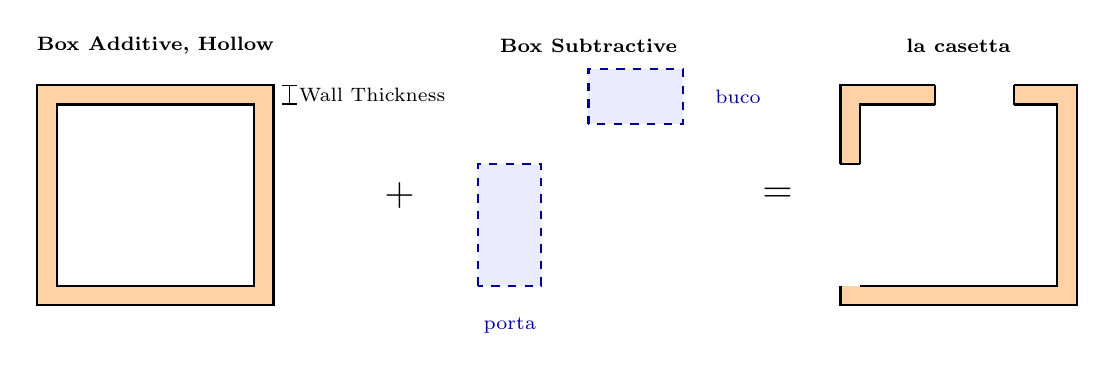
\begin{tikzpicture}[font=\footnotesize, x=1cm, y=1cm]
  % box additiva hollow (sezione)
  \node[font=\scriptsize\bfseries] at (1.5,3.3) {Box Additive, Hollow};
  \fill[orange!35] (0,0) rectangle (3,2.8);
  \fill[white] (0.25,0.25) rectangle (2.75,2.55);
  \draw[thick] (0,0) rectangle (3,2.8); \draw[thick] (0.25,0.25) rectangle (2.75,2.55);
  \draw[|-|, thin] (3.2,2.55) -- node[right, font=\scriptsize]{Wall Thickness} (3.2,2.8);
  \node at (4.6,1.4) {\Large $+$};
  % sottrattive
  \node[font=\scriptsize\bfseries] at (7.0,3.3) {Box Subtractive};
  \draw[thick, dashed, blue!60!black, fill=blue!8] (5.6,0.25) rectangle (6.4,1.8);
  \node[font=\scriptsize, blue!60!black] at (6.0,-0.25) {porta};
  \draw[thick, dashed, blue!60!black, fill=blue!8] (7.0,2.3) rectangle (8.2,3.0);
  \node[font=\scriptsize, blue!60!black] at (8.9,2.65) {buco};
  \node at (9.4,1.4) {\Large $=$};
  % risultato
  \begin{scope}[xshift=10.2cm]
    \node[font=\scriptsize\bfseries] at (1.5,3.3) {la casetta};
    \fill[orange!35] (0,0) rectangle (3,2.8);
    \fill[white] (0.25,0.25) rectangle (2.75,2.55);
    \fill[white] (-0.05,0.25) rectangle (0.3,1.8);
    \fill[white] (1.2,2.5) rectangle (2.2,2.85);
    \draw[thick] (0,1.8) -- (0,2.8) -- (1.2,2.8); \draw[thick] (2.2,2.8) -- (3,2.8) -- (3,0) -- (0,0) -- (0,0.25);
    \draw[thick] (0.25,1.8) -- (0.25,2.55) -- (1.2,2.55); \draw[thick] (2.2,2.55) -- (2.75,2.55) -- (2.75,0.25) -- (0.25,0.25);
    \draw[thick] (0,1.8) -- (0.25,1.8); \draw[thick] (1.2,2.55) -- (1.2,2.8); \draw[thick] (2.2,2.55) -- (2.2,2.8);
  \end{scope}
\end{tikzpicture}
\caption{Additive e Subtractive in sezione: una box additiva vuota (Hollow, con il suo
Wall Thickness) e due box sottrattive che la ``bucano'', una per la porta e una per il
buco sul soffitto da cui cadere nella stanza sottostante, come nella casetta costruita a
lezione. Ricostruzione schematica; le proporzioni sono indicative.}
\label{ue13:fig:csg}
\end{figure}

\paragraph{Il però: le brush sono pesanti.} ``Ora c'è un però, e il però è che le brush
sono \textbf{pesanti}.'' Se si riempie una scena di brush, ``perché volete diverse casette e
diverse zone dentro cui entrare'', ``si carica tanto sulla memoria del progetto''. Il
rimedio: \textbf{farla diventare una static mesh}. Nei Details della brush c'è il comando
per creare una static mesh dalla geometria (\emph{Create Static Mesh}, nella parte avanzata
dei Brush Settings), che chiede dove salvarla. Il docente lo fa con la casetta: nel
Content Browser compare ``un bloccone'', ma solo della brush selezionata (``se avessimo
selezionato tutte quante le brush, avremmo avuto un effetto diverso'': la mesh le avrebbe
comprese tutte). Il docente elimina la brush originale, ``non ci serve più'': la static mesh
che resta ``è molto meno pesante. Io posso riempirci la scena di questa roba qua.''
Bisognerebbe solo sistemarne il \textbf{pivot}, ``perché ce l'ho salvato col pivot
strano''. Un consiglio di ordine: invece di ``buttarla qui in mezzo al Content'', come ha
fatto lui, create ``una \emph{new folder} che chiamate, che ne so, \textbf{Blockout
Assets}'', e lì dentro mettete tutto quello che create. (Poi le elimina: a lui non servono.)

\paragraph{Approfondimento: perché le brush pesano, e Create Static Mesh.} Le geometry
brush sono la versione moderna della geometria \textbf{BSP} (\emph{binary space
partitioning}) delle vecchie versioni di Unreal: le brush additive e sottrattive vengono
combinate, nell'ordine in cui sono state create, in un'unica geometria del livello, che
l'editor ricalcola (\emph{Build Geometry}) quando le si modifica. Questa geometria non si
può istanziare, non ha LOD, ha UV e lightmap generate automaticamente e la sua collisione
è meno efficiente di quella di una mesh: per questo, oltre che per la memoria, Epic
raccomanda di usarle per il block out e di convertirle (o sostituirle) con static mesh
nel livello finale. Il comando \textbf{Create Static Mesh} salva la geometria delle brush
selezionate come asset \emph{Static Mesh}, con i materiali delle facce come slot; la
mesh nasce con il pivot all'origine del mondo o della prima brush, che si corregge con il
\emph{Modeling Mode} (strumento \emph{Pivot}) o riposizionandola. Nel libro di Romero e
Sewell le brush non compaiono: il libro costruisce i livelli con static mesh duplicate
(capitolo 9, il pavimento duplicato con Alt e trascinamento per raddoppiare l'area di
gioco). Quanto al modeling tool, il \emph{Modeling Mode} esisteva già come plugin
sperimentale nelle ultime versioni di Unreal~4, ma è con Unreal~5 che è diventato uno
strumento standard dell'editor: la frase del docente è vera nella sostanza. Funzionamento
generale dell'engine, salvo il riferimento al libro.

% ---------------------------------------------------------------------
\section{Le altre forme e il Brush Editing}
\label{ue13:sec:forme}

``Vediamo effettivamente cosa ci permettono di fare le altre brush.'' (La box sottrattiva il
docente se la tiene, ``almeno vediamo''.)

\paragraph{Cone.} Ha sempre le stesse impostazioni per le facce. Nei Brush Settings: un
valore \textbf{Z}, l'altezza; un \textbf{Outer Radius}; un \textbf{Inner Radius}, che non
si può modificare finché il cono non è \textbf{Hollow}: ``se io la rendo vuota'' si vede
com'è dentro, e si crea una struttura ``sulla base di quello che a me serve''. Il docente ci
mette dentro la box sottrattiva: ``una capannola mezza favola, una tenda''. Si può aumentare
il numero di lati (\textbf{Sides}): da 3, ``una piramide, anzi un D4'', fino a 500. A 500
``ha un po' stutterato, e non ci sarà mai un momento in cui ti servirà avere un cono così
preciso'', ma più facce lo rendono ``un po' più smussato''.

\paragraph{Cylinder.} ``Più o meno le stesse cose'': l'altezza, l'Outer Radius (``quanto è
largo effettivamente''), le facce come per il cono, Hollow o no, e il tipo, additivo o
sottrattivo.

\paragraph{Sphere.} Il \textbf{Radius}, ``quanto è ampia'', e la \textbf{Tessellation},
``quanti blocchi ha, quindi quanto è sferica''.

\paragraph{Linear Stair.} Tutto si basa sullo scalino, ``come anche le altre scale'': la
lunghezza del singolo scalino (\textbf{Step Length}), l'altezza (\textbf{Step Height}), la
larghezza (\textbf{Step Width}) e il numero di scalini (\textbf{Num Steps}): ``aumentando
gli scalini, aumenta l'altezza e aumenta la distanza''. Poi \textbf{Add to First Step},
``quanto in alto in più deve essere il primo scalino'': ``vedete, lui alza un tot''.

\paragraph{Curved Stair.} Altezza e larghezza dello scalino, e in più:
\begin{itemize}
  \item l'\textbf{Inner Radius}, il raggio del cerchio interno: ``se è molto largo, le
        scale vengono più arcuate'';
  \item l'\textbf{Angle of Curve}, ``quanto deve curvare la scala'': di default 90 gradi,
        ``però potreste fare anche 180, 270, anche 360 gradi'', se volete ``una singola
        chiocciola'';
  \item Num Steps e Add to First Step, ``esattamente allo stesso modo'';
  \item \textbf{Counter Clockwise}, per le scale ``che vanno nell'altra direzione''.
\end{itemize}
``Con tutte queste, poi potete andare a creare effettivamente delle static mesh.''

\paragraph{Spiral Stair.} ``Gli stessi parametri'': Inner Radius, Step Width, Step Height,
e in più lo spessore del singolo gradino (\textbf{Step Thickness}), ``perché è costruita
proprio a gradoni, ognuno di questi è un oggetto a sé stante, tutti attaccati l'uno con
l'altro''. C'è poi il numero di scalini \emph{per 360 gradi} (\textbf{Num Steps Per 360}):
``se voi dite che devono esserci 33 scalini per fare 360 gradi, poi dovete aggiungere
abbastanza scalini per arrivare a fare 360 gradi''; abbassandolo, con lo stesso numero
totale di scalini (``50, 60'') ne servono meno per fare un giro. Infine si può rendere
liscio il soffitto (\textbf{Sloped Ceiling}) o il pavimento (\textbf{Sloped Floor}), ``e
quindi avere una sorta di scivolo, una rampa'', e Counter Clockwise.

\paragraph{Il Brush Editing.} ``Prima facciamo un'ultima roba'': passare dalla
\textbf{Selection Mode} al \textbf{Brush Editing} (dal menu delle modalità dell'editor). Qui
si fanno ``piccole operazioni di modellazione'': selezionare un \textbf{vertice} e
spostarlo, una \textbf{faccia} e muoverla, un \textbf{edge} e muoverlo, ``in questo modo ci
andiamo a creare esattamente il tipo d'oggetto che serve a noi, anche se la forma che
serve a noi non c'era'' fra le brush. E lo \textbf{Split}: ``fa passare una serie di
vertici e di edge a tagliare'', una sezione dell'oggetto; ``si formano nuove facce, e
queste nuove facce possono essere prese e modificate''. ``Non so quanto spesso vi tornerà
utile fare un ecomostro del genere, però avete la possibilità di farlo.'' Un'avvertenza
emersa dalla prova: dopo le modifiche, l'oggetto ``è ancora una brush'', ma ``appena
l'andiamo a modificare'' dai Brush Settings ``ritorna come era precedentemente'': i
parametri ricostruiscono la forma da zero e cancellano le modifiche manuali.

\begin{table}[htbp]
\centering
\small
\begin{tabular}{@{}p{2.5cm}p{11.5cm}@{}}
\toprule
\textbf{Brush} & \textbf{Parametri (Brush Settings)} \\
\midrule
tutte & Brush Type: Additive / Subtractive; i materiali e le UV si impostano per faccia \\
Box & X, Y, Z; Wall Thickness (default 10); Hollow; Tessellated (solo se non hollow) \\
Cone & Z (altezza); Cap Z; Outer Radius; Inner Radius (solo se hollow); Sides (da 3 a
500); Align to Side; Hollow \\
Cylinder & Z; Outer Radius; Inner Radius (solo se hollow); Sides; Align to Side; Hollow \\
Sphere & Radius; Tessellation \\
Linear Stair & Step Length; Step Height; Step Width; Num Steps; Add to First Step \\
Curved Stair & Inner Radius; Step Height; Step Width; Angle of Curve (default
90$^\circ$); Num Steps; Add to First Step; Counter Clockwise \\
Spiral Stair & Inner Radius; Step Width; Step Height; Step Thickness; Num Steps Per 360;
Num Steps; Sloped Ceiling; Sloped Floor; Counter Clockwise \\
\bottomrule
\end{tabular}
\caption{Le geometry brush e i loro parametri. I nomi sono quelli dei Details di Unreal
Engine~5; quelli non letti a lezione (Cap Z, Align to Side) sono completati come
approfondimento.}
\label{ue13:tab:brush}
\end{table}

``Sono le cinque e mezza.'' Il docente annuncia che, al ritorno dalla pausa, si potrebbe
fare ``un piccolo block out utilizzando gli oggetti che avete'': le brush, le static mesh e
gli oggetti fatti con Igor, ``per cui magari vi piazzate dei collectible da raggiungere in
giro'', ``anche molto semplice''. Pausa di un quarto d'ora: ``facciamo 45''.

% ---------------------------------------------------------------------
\section{La pausa e la scelta del formato}
\label{ue13:sec:pausa}

(Durante la pausa la trascrizione contiene solo il blocco di testo ripetuto citato
nell'introduzione.) Alla ripresa c'è un problema di volume (``stavo leggendo il messaggio
che aveva scritto Augusto in chat'') e l'appello: Federico c'è, Guido ``c'è, ma non gli
funziona la telecamera'' (``basta che siete responsivi'').

\paragraph{La domanda del docente.} ``Ci stavo pensando adesso che stavamo fermi'': come
preferiscono strutturare le lezioni?
\begin{enumerate}
  \item una prima parte di spiegazione e una seconda in cui gli studenti ``provano a
        costruire qualcosa'', magari in streaming, ``così gli altri vedono anche cosa
        fate'' e il docente può commentare;
  \item tutte e tre le ore di spiegazione, con il lavoro pratico fra una lezione e l'altra
        e i feedback all'inizio della lezione successiva. Il tempo a disposizione cambia:
        ``da oggi, che è giovedì, fino a martedì avrete più tempo; da martedì a giovedì ne
        avrete meno''.
\end{enumerate}
Un primo studente preferisce la prima opzione, ``perché almeno abbiamo dei feedback diretti
e ci si può soffermare di più sulle varie cose''. Un altro la seconda, ``perché forse
riusciamo a fare più cose'', ``vediamo un po' più di argomenti''. Il docente avverte che le
cose che si faranno con lui ``sono tendenzialmente non troppo complesse, è più una
questione di metterle assieme'', e che non vorrebbe la situazione in cui ``io vi dico
facciamo questa cosa, la prossima volta me lo fate vedere e nessuno fa niente''. Edoardo,
alle prese con il caldo, dice che fare le cose fra una lezione e l'altra ``non è un peso''
se trova una soluzione; un altro: ``personalmente mi piace la seconda''. Il voto (``siete
dispari, quindi uscirà fuori una verità o l'altra''; ``per chi ci guarda da casa sarà tutto
in mano alle persone che erano qui'') premia la \textbf{seconda}: ``Tommaso, indipendentemente
dal tuo input, il popolo ha deciso di riempire la lezione con delle cose che magari faccio
io''.

Conseguenze: la lezione sullo \textbf{speed level design} andrà ``rimaneggiata'', ``perché
non so quanto ha senso che io mi metta a fare uno speed level per tre ore con voi che mi
guardate''; era ``una roba che mi sarebbe piaciuto far fare a voi''. Per la volta successiva,
a chi vuole, il docente chiede ``un piccolo livellino'' con geometrie e static mesh, ``per
giocare un po''': ``è molto bello sapere come funziona Unreal, però deve esserci del
\textbf{divertimento} nella creazione. Io mi devo divertire mentre creo il gioco.'' Le
indicazioni precise arrivano a fine lezione (sezione~\ref{ue13:sec:compiti}).

\paragraph{Che cosa fare nell'ora rimasta.} Personalizzare i parametri del bot in una gym
``è relativamente fine a se stesso'', ``un discorso abbastanza semplice'' che gli studenti
possono fare da soli. Meglio un altro actor interessante: le \textbf{luci}, e ``se riesco,
un accennino di post process''. Le luci si vedranno ``in un vuoto'', ``senza un dressing già
finito'', e si riprenderanno quando si parlerà di \emph{enrichment}, di dressing e di
ambienti, con lo speed level; per quella lezione il docente potrebbe preparare
``un ambientino'' o passare un pacchetto, ``così chi vuole lo fa assieme a me''. Le slide
non servono: ``faremo a braccio''. (Di nuovo problemi con Zoom: ``ogni volta che parto con la
stream non funziona il tasto destro''.) Il docente costruisce con una grande box un
ambientino chiuso (``così abbiamo un po' d'ombra''), invitando Filippo, che preferiva fare
le cose insieme, a sperimentare in parallelo. (Una parte della costruzione, nella
trascrizione, è incomprensibile: ``me la metà? E questa la facciamo? Giusto per fare
razzola''.)

% ---------------------------------------------------------------------
\section{Le luci: i tipi e la mobility}
\label{ue13:sec:mobility}

``Cos'è che non sta più funzionando in quella zona lì?'' Dentro la box: ``la luce del sole'',
risponde uno studente. La luce del sole è un tipo di luce, ``la signora
\textbf{Directional Light}''. Le luci di Unreal sono cinque: \textbf{Directional},
\textbf{Point}, \textbf{Spot}, \textbf{Rect} e \textbf{Sky Light}. Secondo la classificazione
del docente:
\begin{itemize}
  \item directional e sky light sono \textbf{luci ambientali};
  \item point e spot light si usano ``principalmente per l'illuminazione'';
  \item la rect light ``principalmente per i riflessi o per delle luci specifiche''.
\end{itemize}

\paragraph{Il costo dei rimbalzi.} ``Una cosa importante da dire è che il modo in cui Unreal
calcola le luci è simulando delle onde'' e il modo in cui ``queste onde luminose rimbalzano
sulle superfici''. Ci saranno situazioni in cui a una luce verranno chiesti ``troppi
rimbalzi, che equivalgono a troppi calcoli, che equivalgono a un peso molto elevato'':
bisogna stare attenti a come si posizionano le luci. (Sull'idea delle ``onde'' si veda
l'approfondimento alla fine della sezione.)

\paragraph{La Mobility.} ``Un parametro fondamentale che c'è in tutte le luci'' è la
\textbf{Mobility}: di default le luci sono \textbf{Stationary}, ma ci sono anche
\textbf{Static} e \textbf{Movable}. ``Non mi aspetto una risposta super completa, voglio
vedere se riusciamo ad arrivarci'' (``basta che ci passate sopra col mouse e ve lo dice
cosa fanno, però state con me''). Le ipotesi degli studenti: movable ``sarà tipo la luce di
una macchina''; stazionaria ``che sta ferma e non si muove'', ma statica ``mi sembra simile
come significato''; un altro propone ``statica un lampione, stazionaria il faro di una
macchina ferma, che potenzialmente si può muovere''; un altro ancora che la movable
``dovrebbe avere delle proprietà fisiche, magari condizionata dalla gravità'' (``la gravità
non c'entra''); un altro l'angolazione (``no, l'angolazione dipende dal tipo di luce che
utilizziamo''). Il docente rinuncia alla prova pratica (``qui c'è un po' di fregatura,
perché siamo in preview'') e parte dagli usi:
\begin{itemize}
  \item una luce \textbf{movable} è quella di ``una torcia a mano'', di una torcia
        elettrica che si punta, dei fari di una macchina, delle luci di un aereo: ``qualcosa
        in movimento'';
  \item una luce \textbf{stazionaria} è quella di un lampione, di un soffitto, ``di una
        qualsiasi luce di una casa'' \emph{dentro} il livello;
  \item una luce \textbf{statica} serve agli stessi scopi della stazionaria, ``ma fuori dal
        vostro livello''.
\end{itemize}
``Cosa cambia fra statica e stazionaria?'' Uno studente: ``nella stazionaria ci può
interagire un actor come il character''. ``Esatto.'' Le proprietà sono due: se si muove la
luce, l'ambiente reagisce?; se si passa davanti alla luce, la luce reagisce?
(figura~\ref{ue13:fig:mobility}):
\begin{itemize}
  \item la luce \textbf{statica} ``viene cucinata sulla scena'': è \emph{baked}
        completamente nell'editor e non si può modificare in gioco. Quando si
        \emph{buildano} le luci o si esporta il livello, ``la luce viene bakeata ed è
        impressa sulla scena''. Se si sposta l'actor della luce, la luce ``rimane dove è
        stata bakeata''; se il character ci passa davanti, la luce non reagisce. Si usa ``in
        tutti quei posti in cui so che non avrà interazioni e sarà soltanto luce
        d'atmosfera, luce d'ambiente''. È ``il tipo di luce più leggero'';
  \item la luce \textbf{stazionaria} ``se la muovo si rompe, ma se sta ferma e io ci passo
        davanti interagisce con me'': il character proietta ombre corrette, ma se si sposta
        la luce dopo il bake, la luce non si aggiorna;
  \item la luce \textbf{movable} ``fa entrambe le cose'': è completamente dinamica, reagisce
        agli oggetti e può essere spostata ``senza nessun problema''.
\end{itemize}

\begin{figure}[htbp]
\centering
\begin{tikzpicture}[font=\footnotesize, x=1cm, y=1cm,
  ue13col/.style={draw, thick, rounded corners=3pt, minimum width=4.0cm, minimum height=0.8cm,
                  align=center}]
  \node[ue13col, fill=gray!15] (st) at (0,0) {\textbf{Static}};
  \node[ue13col, fill=yellow!30] (sy) at (4.6,0) {\textbf{Stationary} (default)};
  \node[ue13col, fill=orange!30] (mv) at (9.2,0) {\textbf{Movable}};
  \node[align=left, anchor=north, text width=4.0cm] at (0,-0.6)
    {\textbf{bake}: sì, tutta\\ \textbf{si sposta in gioco}: no\\ \textbf{ombre dei personaggi}: no\\
     \textbf{costo}: il più basso\\[2pt] \emph{luce d'ambiente fuori dall'area di gioco}};
  \node[align=left, anchor=north, text width=4.0cm] at (4.6,-0.6)
    {\textbf{bake}: sì, la parte fissa\\ \textbf{si sposta in gioco}: no\\ \textbf{ombre dei personaggi}: sì\\
     \textbf{costo}: medio\\[2pt] \emph{lampioni, luci di casa, soffitti}};
  \node[align=left, anchor=north, text width=4.0cm] at (9.2,-0.6)
    {\textbf{bake}: no\\ \textbf{si sposta in gioco}: sì\\ \textbf{ombre dei personaggi}: sì\\
     \textbf{costo}: il più alto\\[2pt] \emph{torce, fari, luci di un aereo}};
  \draw[-{Stealth[length=2.5mm]}, very thick, gray] (-2.0,-3.3) -- node[below, font=\scriptsize]{più dinamica, più pesante} (11.2,-3.3);
\end{tikzpicture}
\caption{Le tre Mobility delle luci come le descrive il docente: che cosa viene
precalcolato (\emph{baked}), se la luce si può spostare in gioco, se reagisce ai personaggi
che le passano davanti, quanto pesa e per che cosa si usa.}
\label{ue13:fig:mobility}
\end{figure}

\paragraph{Approfondimento: onde, raggi e Lumen.} L'immagine delle ``onde'' è una
semplificazione del docente: Unreal non simula la luce come un'onda (niente interferenza o
diffrazione), ma come energia che viaggia in linea retta e rimbalza, cioè per
\emph{raggi}. Il calcolo dei rimbalzi (l'illuminazione \emph{globale}) avviene in due modi:
precalcolato, con \textbf{Lightmass}, che scrive il risultato nelle \emph{lightmap} delle
superfici al momento del build (luci static e stationary); o in tempo reale, con
\textbf{Lumen}, il sistema di illuminazione globale dinamica che Unreal Engine~5 attiva di
default nei progetti nuovi. Il principio del docente resta valido: più superfici e più
luci si sovrappongono, più calcoli servono, che siano fatti una volta nel build o a ogni
frame. Sulla stationary, un dettaglio in più: in gioco se ne possono cambiare colore e
intensità (non la posizione), e le ombre che proietta sugli oggetti fermi sono precalcolate,
mentre quelle degli oggetti in movimento sono dinamiche. Romero e Sewell (capitolo 4)
mettono la \emph{Mobility} di una point light a \textbf{Movable} proprio ``per poter
cambiare le proprietà della luce durante l'esecuzione'', quando la accendono e la spengono
da Blueprint. Funzionamento generale dell'engine, salvo il riferimento al libro.

% ---------------------------------------------------------------------
\section{La directional light e la sky light}
\label{ue13:sec:directional}

Il docente porta la directional light e la sky light ``tutte nello stesso posto''.
``Spostare queste luci non ha nessun tipo d'effetto.'' Perché?

\paragraph{La Directional Light.} Si può muoverla e scalarla ``come voglio e non cambia
assolutamente nulla. Ma se la ruoto, la luce reagisce.'' (``In questo caso reagisce anche''
un altro actor del cielo, ``perché è collegato'': la trascrizione dice ``la Schakespeare'' e
``la Schiapunsky'', con ogni probabilità la \emph{Sky Sphere} o la \emph{Sky Atmosphere}
del livello; il nome esatto non è ricostruibile.) La ragione: ``la directional light è
composta in una maniera abbastanza peculiare: è un \textbf{fascio di rette parallele} che
prende tutta la scena''. Spostarla non cambia nulla; ruotarla cambia ``il modo in cui viene
indirizzata la luminosità''. I parametri interessanti:
\begin{itemize}
  \item l'\textbf{Intensity}: aumentandola, ``va in questo caso a bruciare un pochino tutta la
        scena'' (``l'intensità della luce calcolata in X'': l'unità di misura nella
        trascrizione è incomprensibile; per la directional è il \emph{lux});
  \item il \textbf{Light Color}: una ruota dei colori per il colore della luce, la sua
        saturazione, ``quanto sarà scura, magari quanto sarà livida''. Se si vuole che più
        luci abbiano lo stesso colore, si copia il codice \textbf{Hex Linear} e lo si incolla
        nelle altre, ``il modo più comodo piuttosto che cercare a mano di replicare la stessa
        luce'': per esempio un corridoio in cui tutte le torce sono ``molto calde, molto
        accese, molto infuocate'';
  \item la \textbf{Temperature} (con \emph{Use Temperature}), per una luce ``tendenzialmente
        più calda o più fredda''; ``così, se volete fare \emph{Breaking Bad} quando sono in
        Messico, tutto giallo'';
  \item \textbf{Affects World}: ``questa luce che sto utilizzando ha effetto sul mondo? È una
        luce attiva o disabilitata?''. Serve, per esempio, a vedere ``come contribuisce alla
        scena'' una luce alla volta;
  \item \textbf{Cast Shadows}: la luce illumina comunque, ma proietta le ombre solo se è
        attivo;
  \item la \textbf{Dynamic Shadow Distance}: secondo il docente, ``quanto precisamente
        viene calcolata l'ombra, quanto è netta''. ``Non può essere notato adesso perché
        stiamo utilizzando solo geometrie''; con asset veri un valore basso si nota. Il
        docente cerca nel progetto una mappa già arredata per mostrarlo (``mi sa che non ne
        abbiamo, a parte quelle che ha fatto Igor'') e rimanda: ``la prossima volta mi
        preparo una scenetta carina a livello estetico''. È un parametro che ``tende ad
        appesantire un pochino le scene'', ma ``l'effetto che fa è talmente meglio rispetto a
        non averlo'': ``giocatevi un po' di potenza in più''.
\end{itemize}

\paragraph{Una sola per scena.} ``Non dovete mai avere \textbf{due directional} nella stessa
scena'': l'engine prova a calcolarle entrambe, ``fa molta fatica'' e ``il risultato è
tremendo'', con problemi di ombre calcolate in direzioni diverse. Allo stesso modo
``evitate di avere due sky sphere'', anzi, si corregge, due \textbf{sky light}: ``skylight e
directional light, una soltanto per scena''.

\paragraph{La Sky Light.} ``Funziona in maniera un po' diversa'', ``un po' più complessa'', e
``al momento non ci serve troppo indagarla''. Che cosa fa: ``è la luce che dà il
\textbf{mood}, la diffusione'', ``va a colorare l'aria, va a dare colore alla scena''. Si vede
cambiando il colore della sky light: cambiano di colore le \emph{ombre}. Per una scena al
tramonto, ``piuttosto che avere solo la directional che è arancione'', si media fra
directional e sky light, ``più tutta una serie di altre cose, perché utilizzeremo anche il
post process'' (la volta successiva). Fra i parametri, oltre all'intensità, quelli
dell'\textbf{ambient occlusion}: la distanza massima (\emph{Occlusion Max Distance}), il
contrasto (\emph{Contrast}) e ``quanto è moltiplicata'' (\emph{Occlusion Exponent} e
\emph{Min Occlusion}); e anche qui Cast Shadows e Affects World. ``Principalmente, mood
della scena e ambient occlusion.''

\paragraph{Approfondimento: Dynamic Shadow Distance, e due directional.} Il nome completo
del parametro è \emph{Dynamic Shadow Distance Movable Light} (o \emph{Stationary Light}, a
seconda della mobility): è la distanza dalla camera entro cui la directional disegna le
ombre dinamiche, divise in \emph{cascate} (\emph{Cascaded Shadow Maps}) di risoluzione
decrescente. Non è quindi la ``nettezza'' in sé, ma lo spazio su cui la risoluzione delle
ombre viene distribuita: oltre quella distanza le ombre dinamiche spariscono (restano solo
quelle precalcolate), e allungarla, a parità di cascate, rende le ombre vicine meno
dettagliate. In Unreal Engine~5, con le \emph{Virtual Shadow Maps} attive di default, questo
compromesso pesa molto meno. Sulle due directional, la regola del docente è la pratica
comune; a rigore Unreal ne supporta due solo come sole e luna dell'atmosfera (indice
\emph{Atmosphere Sun Light Index} 0 e 1), un caso particolare. Funzionamento generale
dell'engine.

% ---------------------------------------------------------------------
\section{Point light e spot light}
\label{ue13:sec:point}

``Passando a delle luci con cui andrete a smanettare molto ma molto di più'': le luci
``antropiche'', quelle che si useranno ``per fare quasi tutto'', \textbf{point light} e
\textbf{spot light}. ``Fra le due, qual è più leggera, più facile da calcolare,
indipendentemente dalla mobility?''

\paragraph{La domanda.} Uno studente risponde la point light, ``perché non si va a calcolare
anche la direzione''. ``È esattamente il contrario.'' La point light è a 360 gradi: ``lui
calcola contemporaneamente tutte le direzioni''. La \textbf{spot light} è più leggera
``perché non va a calcolare i rimbalzi della luce nelle altre direzioni'': ``la discriminante
è quella della direzione''. In una scena affollata, la spot illumina solo dove la si punta,
mentre la point ``va posizionata con attenzione perché va a colpire anche gli oggetti che ha
alle spalle'', ``indiscriminatamente dalla direzione''.

\paragraph{L'Attenuation Radius.} Per la point light, ``i due parametri più importanti sono
l'intensità e l'\textbf{Attenuation Radius}'', la sfera che si vede attorno alla luce.
``Indipendentemente dal fatto che io ho messo 10.000 miliardi di intensità, se il raggio non
tocca nulla la luce non illumina'' (o meglio, illumina solo dentro la sfera, ``quindi non
rimbalza su niente''). È ``il raggio massimo entro cui la luce avrà effetto'', e gestisce
un'attenuazione dalla sorgente fino al bordo: il \emph{gradiente} della luce. Con
un'intensità altissima, per un'attenuazione sensata bisogna ingrandire molto il raggio. Ma
anche con un'intensità bassa l'attenuazione arriva fino al bordo, e questo è il punto: il
raggio è ``il parametro che va gestito con attenzione'', ``perché determina con quanti
oggetti la luce andrà a compenetrare'', e quindi quante ombre dovrà proiettare. ``Anche se
l'intensità è molto bassa, nel momento in cui questo muro è all'interno del raggio,
l'engine dovrà calcolare'' l'ombra e la luce su quella superficie.

\paragraph{La X rossa.} ``Una cosa che vi capiterà sicuramente'': una luce con una
\textbf{X rossa} sopra. Il docente la riproduce mettendo più luci vicine (al primo tentativo
``non abbastanza'': i raggi erano piccoli). Vuol dire che ``l'engine ha rinunciato a far
proiettare ombre a questa luce'': la luce illumina comunque, ``ma non proietta ombre perché
ci sono troppe altre luci con cui questa luce sta compenetrando''. L'engine lo segnala come
problema, ``non grave''. I rimedi sono due: dire noi alla luce di non proiettare ombre
(Cast Shadows disattivato), così l'engine ``non cercherà costantemente di proiettarle'';
oppure \textbf{ridurre il raggio} ``a tal punto da non farlo compenetrare con troppe cose''.
``Non riempite la vostra scena di luci, piuttosto utilizzate \textbf{poche luci molto
significative}.''

\paragraph{Il corridoio.} L'esempio: un corridoio con una fila di luci. Mentre il
personaggio passa, le ombre sono corrette ``fino a che non arriviamo qui vicino'': lì la
luce viene calcolata ``come se questa non ci fosse'', e l'ombra viene proiettata dalle due
luci ai lati. ``Vedete, qui skippa, qui salta'': l'ombra della luce con la X non c'è, c'è
solo quella della luce ``un po' più lontana'', mentre altrove l'ombra è ``molto più forte,
molto più precisa, molto più netta''. ``Se replicate questo esperimento per conto vostro, vi
rendete conto che è abbastanza semplice da replicare.''

\paragraph{La sorgente: Source Radius, Soft Source Radius, Source Length.} Come illuminare
un corridoio ``piuttosto che avere una luce per torcia, una luce per punto''? Si modifica la
\textbf{sorgente}: ingrandendo il \textbf{Source Radius} e allungando la \textbf{Source
Length}, la luce non parte più da un punto ma ``da un cilindro, da una capsula'', ed è
``più distribuita''. Il raggio può anche essere zero, ``se volete una linea e basta''. È
così che si fanno illuminazioni particolari, ``tipo un locale illuminato unicamente dalla
luce dei \textbf{neon}'': mesh con materiali \textbf{emissive}, ``che quindi già emettono una
piccola luce di loro'', più luci distribuite ``in maniera più omogenea'' in questo modo. Il
\textbf{Soft Source Radius} ``serve per creare un'altra lucina interna, come quando puntate
una torcia verso il muro'': una parte più attenuata all'esterno e una meno attenuata
all'interno (``si vede meglio con la spot''; il docente non riesce a mostrarlo bene). Più
sotto ci sono di nuovo Affects World e Cast Shadows, e lo \emph{scattering} con la nebbia
volumetrica (\emph{Volumetric Scattering Intensity}), che servirà quando si userà una
nebbia (la trascrizione dice ``una FOD'', con ogni probabilità \emph{fog}); poi ``molti, molti
parametri'' per le ombre (risoluzione, comportamento sulle pendenze). ``Non tutti vi
servono'', ``a meno che non vogliate fare proprio il \emph{light artist}''. (``Non l'ho
detto prima'': anche la point light ha il Light Color, ``per fare le vostre luci da inferno,
da nightclub, da \emph{Night City}''.)

\paragraph{La spot light.} È fatta a \textbf{cono}, quindi si ruota. Intensità e Light
Color come le altre; l'\textbf{Attenuation Radius}, qui, ``non dipende da quanto è la
sfera, ma è la lunghezza del cono'', ``quanto in là viene proiettata'': ``se sta così non
colpisce il muro, così illumina questa parte del muro''. Poi due angoli
(figura~\ref{ue13:fig:luci}):
\begin{itemize}
  \item l'\textbf{Outer Cone Angle}, che gestisce il cono;
  \item l'\textbf{Inner Cone Angle}, il cono interno, ``l'effetto torcia'': nella parte
        colpita dall'inner cone ``ci sarà una minore attenuazione''. Con i due angoli vicini
        il bordo è netto; ``volendo potete avere anche un cono che non attenua mai alla
        base, che attenua soltanto sulla distanza''. Questo cono serve a determinare la
        \emph{sfumatura}, ``ed è anche quello che faceva l'altro nella point, ma con questo
        si nota meglio''.
\end{itemize}
Anche qui Source Radius, Source Length e Soft Source Radius, e i parametri delle ombre.

\paragraph{La domanda sull'effetto accecante.} Uno studente chiede se, guardando
direttamente la luce, ci sia ``l'effetto accecante''. ``No, assolutamente no.'' L'effetto
``tipo quando guardi il sole'' si crea con il \textbf{post process}, che il docente vuole
far vedere ``quando abbiamo una mappa che non sia soltanto delle geometrie'' (con un
pacchetto di mesh e mappe già fatte: ``sono abbastanza sicuro che questo pacchetto dovesse
avere delle mappe''). Con i parametri del post process si aggiungono \textbf{bloom} e
\textbf{lens flare}. Altro esempio: i \textbf{god rays} (``god shaft''), ``una luce molto
forte che entra dalla finestra e c'è questa proiezione luminosa che taglia la scena''.
``Quella roba lì con la luce non puoi farla. Ti serve la luce, ma devi andare a manipolare
il modo in cui la telecamera vede la luce con la post produzione.'' Per questo ``la post
produzione va fatta dopo le luci'': ``prende l'illuminazione della scena e ci aggiunge delle
lenti, degli effetti''. Fra le ``lenti'', oltre al bloom: la messa a fuoco, la distorsione,
la \emph{chromatic aberration}.

\begin{figure}[htbp]
\centering
\begin{tikzpicture}[font=\footnotesize, x=1cm, y=1cm]
  % point light
  \node[font=\scriptsize\bfseries] at (1.6,3.4) {Point Light};
  \shade[inner color=yellow!70, outer color=white] (1.6,1.6) circle (1.5);
  \draw[dashed, thick, orange!70!black] (1.6,1.6) circle (1.5);
  \fill[orange] (1.6,1.6) circle (0.08);
  \draw[-{Stealth[length=1.6mm]}] (1.6,1.6) -- (2.66,2.66);
  \node[font=\scriptsize, align=center] at (1.6,-0.5) {Attenuation Radius = sfera;\\360$^\circ$: colpisce anche\\ciò che ha alle spalle};
  % spot light
  \begin{scope}[xshift=4.4cm]
    \node[font=\scriptsize\bfseries] at (1.6,3.4) {Spot Light};
    \fill[yellow!25] (0.2,2.8) -- (3.2,0.2) -- (0.9,0.0) -- cycle;
    \fill[yellow!65] (0.2,2.8) -- (2.55,0.4) -- (1.55,0.1) -- cycle;
    \draw[dashed, thick, orange!70!black] (0.2,2.8) -- (3.2,0.2);
    \draw[dashed, thick, orange!70!black] (0.2,2.8) -- (0.9,0.0);
    \fill[orange] (0.2,2.8) circle (0.08);
    \node[font=\scriptsize, anchor=west] at (2.7,1.3) {Outer Cone};
    \node[font=\scriptsize, anchor=west, fill=white, inner sep=1pt] at (1.25,1.15) {Inner};
    \node[font=\scriptsize, align=center] at (1.6,-0.5) {Attenuation Radius =\\lunghezza del cono};
  \end{scope}
  % rect light
  \begin{scope}[xshift=8.8cm]
    \node[font=\scriptsize\bfseries] at (1.8,3.4) {Rect Light};
    \fill[yellow!30] (0.9,2.4) -- (2.7,2.4) -- (3.4,0.2) -- (0.2,0.2) -- cycle;
    \draw[very thick, fill=orange!60] (0.9,2.4) rectangle (2.7,2.6);
    \draw[very thick, gray!70!black] (0.9,2.4) -- (0.55,1.95);
    \draw[very thick, gray!70!black] (2.7,2.4) -- (3.05,1.95);
    \node[font=\scriptsize, anchor=east] at (0.55,2.0) {Barn Door};
    \node[font=\scriptsize, align=center] at (1.8,-0.5) {Source Width $\times$ Height;\\Barn Door Angle e Length};
  \end{scope}
\end{tikzpicture}
\caption{Le tre luci locali e i parametri che ne determinano la forma: la sfera di
attenuazione della point light, i due coni della spot light (nel cono interno
l'attenuazione è minore) e la sorgente rettangolare della rect light, con le ``porte da
stalla'' che ne restringono il fascio. Schema indicativo, non in scala.}
\label{ue13:fig:luci}
\end{figure}

\paragraph{Approfondimento: la X rossa, il costo delle ombre e i god rays.} La X rossa ha
una causa precisa: è il limite delle luci \textbf{stationary} sovrapposte. Le ombre
precalcolate delle stationary vengono scritte in quattro canali di una texture, quindi in
un punto qualsiasi del livello possono sovrapporsi al massimo \textbf{quattro} luci
stationary con le ombre attive (la directional conta come una); la quinta, segnata con la X
rossa, ripiega sulle ombre interamente dinamiche, più costose, o le perde (l'editor la
elenca nel \emph{Map Check}). Per questo i rimedi del docente funzionano: ridurre
l'Attenuation Radius toglie la sovrapposizione; disattivare Cast Shadows toglie la luce dal
conteggio; un'altra via è rendere la luce static o movable. Sul costo: la ragione per cui
una spot light è più economica di una point light sta soprattutto nelle ombre, perché una
spot proietta le ombre con una sola \emph{shadow map} orientata, mentre una point light ne
ha bisogno in tutte le direzioni (una \emph{cube map} di sei facce). Sui \textbf{god rays},
la frase del docente va presa nel suo senso: in Unreal l'effetto si ottiene con le opzioni
\emph{Light Shaft Occlusion} e \emph{Light Shaft Bloom} della directional light, o con la
\emph{Exponential Height Fog} con la nebbia volumetrica attiva; i light shaft sono
comunque un effetto calcolato sull'immagine della camera, quindi della stessa natura del
post process, come dice il docente. L'abbagliamento guardando il sole viene dal
\textbf{bloom} e dall'\textbf{esposizione automatica} (\emph{Eye Adaptation}), entrambi
impostati in un \textbf{Post Process Volume}. Romero e Sewell (capitolo 9) ricordano che il
\emph{Post Process Volume} e il \emph{Lightmass Importance Volume} del livello ``vanno
scalati per coprire l'area di gioco'' quando la si allarga, ``perché servono per
l'illuminazione e gli effetti''; e nel capitolo 12 che la qualità del post processing
(``motion blur e bloom'') e delle ombre (``i dettagli delle ombre hanno spesso un impatto
drammatico sulle prestazioni'') è fra le impostazioni di \emph{Engine Scalability}.
Funzionamento generale dell'engine, salvo i riferimenti al libro.

% ---------------------------------------------------------------------
\section{La rect light}
\label{ue13:sec:rect}

``Ora mi sono scordato le rect light.'' ``Sono un po' strane'': sembrano ``una spotlight,
ma tipo rettangolare'', e invece sono diverse. Si usano principalmente per le
\textbf{illuminazioni industriali}, ``le classiche luci quadrate da fabbrica'', o ``molto
più spesso'' per i \textbf{riflessi}: ``il riflesso della televisione su un pavimento''.
Vanno usate ``soltanto su oggetti rettangolari'' che proiettano una luce specifica, ``come
un'insegna al neon, di quelle dei locali''. ``Se devo farmi calcolare dei riflessi, lo
faccio utilizzando la rect light perché dà dei risultati più precisi.''

I parametri ``non sono troppo diversi'': intensità, colore, Attenuation Radius ``che ormai
abbiamo imparato a conoscere'', la larghezza e l'altezza della sorgente (\emph{Source Width},
\emph{Source Height}). Ciò che cambia:
\begin{itemize}
  \item il \textbf{Barn Door Angle}: la sorgente è un rettangolo centrale ``più una
        struttura lungo il rettangolo'', che Unreal chiama \emph{barn door} (``come si
        traduce?'', chiede il docente; ``la stalla'', risponde uno studente: le alette dei
        proiettori da set, dette appunto \emph{porte da stalla}). Cambiando l'angolo è
        ``come se ci fosse un'ostruzione'': le alette si piegano e la luce va solo in avanti;
        al massimo, la luce arriva fino a terra; nel mezzo, un effetto sfumato;
  \item la \textbf{Barn Door Length}, ``quanto è grande questa lente'', per ``un effetto tipo
        i riflettori degli stadi'', che illuminano ``una parte specifica, molto tagliata,
        molto netta'';
  \item la \textbf{Source Texture}: ``la texture che noi andiamo a inserire diventa il tipo di
        luce che viene messo'', come un'insegna o un televisore che proietta una luce
        particolare; ``è come se andasse a proiettare la luce attraverso un filtro, per
        spiegarlo in modo brutto''. Il docente cerca una texture riconoscibile nel progetto
        (``queste non vanno bene'') senza trovarla, e l'esempio resta a parole;
  \item anche qui la Temperature e Affects World.
\end{itemize}

% ---------------------------------------------------------------------
\section{Il build delle luci e i riflessi}
\label{ue13:sec:build}

``Stavo per scordare una delle parti fondamentali.'' La differenza fra static, stationary e
movable si vedeva ``molto meglio sulla quarta edizione''; ma anche sulla quinta ``dovete
stare attenti'': ``vi capiterà di fare dei livelli in cui avete un'illuminazione, poi andate
a buildare e la luce che vi ritrovate alla fine non è la luce che pensavate di avere''.
Questo perché le luci \textbf{statiche e stazionarie} hanno bisogno di essere
\textbf{buildate}.

\paragraph{La qualità del build.} Quando si fa il build bisogna scegliere la qualità con cui
calcolare le luci (\emph{Lighting Quality}): di default è \textbf{Preview}, ``la qualità
più veloce'', in cui ``vengono calcolati meno rimbalzi''; quando si pubblica un gioco si usa
\textbf{Production}, il livello più alto, che viene calcolato al build e ``rimane bakeato
sul livello''. Se non si fa il build, le luci statiche e stazionarie ``rimangono delle
preview''.

\paragraph{La ``bestemmia''.} ``Oppure utilizzate questa cosa che sto per dire, sarà una
bestemmia: utilizzate \textbf{solo luci movable}.'' Le movable sono pesanti, ``quindi non
utilizzate solo luci movable, chiaramente''; ma per un livello \emph{molto piccolo}, ``in cui
avete 2--3 luci massimo'', e che serve in fretta, avere luci movable ``che sono esattamente
come le vedete alla fine'' può tornare comodo. ``Se dovete illuminare un livello con 20 e
passa luci, non mettete solo luci movable'': mettete luci static e stationary e fate il
build.

\paragraph{Il menu Build.} Si possono buildare diverse cose, ``pezzo per pezzo'': le luci,
le \textbf{reflection capture} (``ecco che mi mancava, i riflessi''), la visibilità statica
(\emph{Precompute Static Visibility}), il \textbf{landscape} (``che poi vedremo la prossima
volta''), e così via; \textbf{Build All Levels} ribuilda tutto. ``Con la quinta edizione,
tutto sommato, ve la cavate'': in Unreal~4, senza il build, ci sarebbero scritte
\textbf{Preview} sparse per la scena e in alto \textbf{Lighting needs to be rebuilt}.
``Se mai vi capita di lavorare su una versione precedente di Unreal, sappiate che quella
scritta in alto è perché non avete buildato le luci''. In ogni caso: ``quando avete finito
il livello fate sempre un build generale''.

\paragraph{Le Reflection Capture.} I riflessi ``sono abbastanza scollegati
dall'illuminazione, ma funzionano in maniera simile'': anche loro sono \textbf{volumi} che
influenzano zone specifiche e vanno buildati. Si trovano fra i volumi: \textbf{Box
Reflection Capture}, \textbf{Planar Reflection} e \textbf{Sphere Reflection Capture}.
Prendendo la sfera, ``semplice da vedere'': ha un raggio di influenza (di default 3000), che
si ingrandisce e si riduce, e vi si possono assegnare mappe specifiche. Quando si fa il
build, ``catturano tutto quello che c'è all'interno della sfera e calcolano i riflessi sulle
superfici riflettenti''.

\paragraph{Quali superfici riflettono?} ``Perché anche se io buildo qui adesso lui non mi
farà vedere niente di diverso?'' Il docente rimanda alla lezione sui materiali: uno studente
ricorda i parametri ``quanto rifletto la luce, l'opacità''. ``Esatto'': i parametri che
contano sono \textbf{Metallic}, \textbf{Specular} e \textbf{Roughness}, ``soprattutto
Specular e Roughness'', che determinano quanto il materiale sarà riflettente. I materiali
della scena di prova non lo sono; con una roughness ``particolarmente bassa'' e una specular
``particolarmente alta'', tutti gli oggetti nell'area di cattura verrebbero riflessi sulle
superfici capaci di rifletterli: ``le pozzanghere, i pavimenti lucidi, gli specchi''. ``Magari
ci ritorniamo nel momento in cui abbiamo un ambiente più costruito, che non sia solo
blocchi.''

\paragraph{Approfondimento: il build in Unreal Engine 5.} Il motivo per cui ``con la quinta
ve la cavate'' è \textbf{Lumen}: nei progetti nuovi di Unreal Engine~5 l'illuminazione
globale e i riflessi sono calcolati in tempo reale, e una scena illuminata da luci movable
(o da stationary e static non ancora buildate) appare già come apparirà in gioco; i livelli
dei template, inoltre, partono spesso senza illuminazione precalcolata. Il build con
Lightmass serve quando si sceglie l'illuminazione precalcolata, di solito per ragioni di
prestazioni (piattaforme mobili, VR, scene molto statiche), e in quel caso valgono tutte le
avvertenze del docente: il build a qualità Production prima di pubblicare, il
\emph{Lightmass Importance Volume} attorno all'area di gioco, e il controllo del messaggio
``Lighting needs to be rebuilt'' (in Unreal~5 segnalato in modo meno vistoso). Anche le
\emph{Reflection Capture} perdono importanza con i riflessi di Lumen, ma restano il
ripiego quando Lumen è disattivato. La Sphere Reflection Capture ha di default un
\emph{Influence Radius} di 3000 unità (30 metri), il valore letto a lezione. Funzionamento
generale dell'engine; il libro di Romero e Sewell non tratta il build delle luci.

% ---------------------------------------------------------------------
\section{I compiti per martedì e la chiusura}
\label{ue13:sec:compiti}

``Abbiamo una decina di minuti.'' Le luci, ``accennate al volissimo'', si rivedranno con il
post process e con lo speed level, ``se riesco a farvi vedere qualcosina, almeno di che
cos'è concettualmente''. Uno studente chiede delle \emph{linee guida} per il lavoro della
volta successiva: ``delle specie di linee guida''. ``Molto fumose, molto generiche, però così
per darvi qualcosina'':
\begin{enumerate}
  \item una \textbf{gym} in cui si sono calcolati i parametri del proprio personaggio ``che
        ritenete importanti per il gameplay''. La Max Sprint Distance da 26 m serve solo se
        nel gioco ci sono cose a tempo: ``se voi volete fare soltanto un platform, magari
        questa cosa non vi serve''. Pensate ``a seconda del tipo di block out che volete
        fare'' e misurate quanto in alto salta, quanto velocemente si muove, quanto lontano
        salta, le differenze fra lo sprint e il salto, magari con una gravità modificata;
        le misure vanno tenute ``da una parte, all'interno del livello in cui andrete a fare
        il block out'';
  \item \textbf{smanettare con i parametri del bot}, BP\_Bot2, ``in modo da avere un tipo di
        esperienza che magari funziona meglio per il vostro gioco''. Esempio in diretta: il
        \textbf{Walkable Floor Angle}, ``44'' di default. Il docente fa delle rampe di
        pendenze diverse: su alcune il bot sale, su una più ripida ``lo fa scivolare giù''.
        Così si possono fare ``delle parti in cui il vostro robot non può andare, che non
        sono semplicemente dei muri''. O una gravità ``meno lunare''; o una camminata più
        veloce: ``io trovo che la camminata di base del robot, per i miei gusti, sia un po'
        lenta, quindi magari l'andrei a modificare''. E, ``una cosa carina'', il
        \textbf{margine di manovra e di errore}: il bot ``salta e non si muove a mezz'aria,
        ha un pessimo controllo a mezz'aria''; con l'\textbf{Air Control} a 1 ``si muove come
        se non fosse in aria''. ``Quanta libertà di movimento voglio dare al mio giocatore? Per
        quale motivo?'' La gym serve anche a rispondere a domande come: ``so che il mio
        personaggio salta 4 metri in avanti e 2 in alto: posso fare questo salto? E se posso
        farlo, è comodo farlo?'';
  \item un \textbf{piccolo block out} in cui l'obiettivo è prendere da \textbf{tre a cinque
        collezionabili}, ``ognuno ottenuto in una maniera diversa'': esplorando,
        saltellando, usando gli oggetti delle lezioni precedenti, ``schivando i colpi della
        mitraglietta'', ``quello che volete''. Serve a familiarizzare ``con l'idea di fare delle
        piccole sfide che il giocatore deve superare per raggiungere degli obiettivi''.
\end{enumerate}
Alla lezione successiva il docente chiederà che cosa è stato modificato e perché: ``poi
magari ci facciamo una chiacchiera sul perché avete deciso di dare quel tipo di parametro
al robottino e cosa volevate farci, che è l'inizio del design: iniziare a pensare a questi
numeri, in che modo influenzano l'esperienza del giocatore''.

Per chi ha problemi di surriscaldamento: ``provateci'', ``stiamo lavorando principalmente con
dei blocchi'', ``non c'è nulla di pesante da un punto di vista grafico''; ``le cose pesanti
verranno più avanti, quando cominceremo a utilizzare elementi estetici''. ``Penso di essermi
mangiato le mie parole tipo infinite volte, però di averle dette talmente tante volte che
era chiaro il concetto.'' Nessuna domanda. ``Ci becchiamo martedì prossimo'': per qualsiasi
cosa, il \textbf{Discord}, anche per mostrare il proprio lavoro.

\paragraph{Approfondimento: il compito visto dai libri.} Il compito mette insieme i temi
della giornata nell'ordine in cui Totten li presenta: prima le metriche (la gym), poi il
whiteblocking (il block out), poi le sfide costruite sulle metriche e sulle abilità del
personaggio. Due criteri dal suo capitolo 2 sono utili come controllo: ogni sfida dovrebbe
usare una metrica misurata (un salto vicino al limite, una distanza vicina alla Max Sprint
Distance, una pendenza oltre il Walkable Floor Angle) e dovrebbe essere \emph{leggibile},
cioè comunicare al primo sguardo se e come si supera, come il blocco da 1,40 m della
lezione. Romero e Sewell (capitolo 13) mostrano come trovare e piazzare rapidamente
actor di supporto dal \emph{Place Actors Panel} (lo stesso pannello usato a lezione per le
brush), comodo per disseminare il livello di collezionabili e punti di riferimento.

% ---------------------------------------------------------------------
\begin{table}[htbp]
\centering
\small
\begin{tabular}{@{}p{4.6cm}p{3.2cm}p{6.2cm}@{}}
\toprule
\textbf{Misura o valore} & \textbf{Valore} & \textbf{Dove e a che serve} \\
\midrule
Max Sprint Distance & 26 m & la corsa con una barra di stamina; limite per inseguimenti e
distanze fra ricariche \\
Margine sullo sprint & circa 20 m & dove mettere una ricarica di stamina \\
Walk Jump / Sprint Jump & 4 m / 6 m & la lunghezza dei salti del bot con Jump Z Velocity
modificata \\
Limiti per i salti di un platform & circa 2,20--2,30 m in alto, 5,80 m in lungo & le sfide
del livello, sotto i massimi \\
Blocchi d'altezza & 1; 1,40; 1,60; 1,80; 2 m & il feeling del salto; 1 m superato
``male'', 1,40 m no \\
Max Step Height & 45 cm (provato con 40 cm e 1 m) & il gradino che si sale camminando \\
Walkable Floor Angle & ``44'' (44,77$^\circ$) & la pendenza oltre cui il bot scivola \\
Jump Z Velocity & 420 $\to$ 700 (poi 600--650) & l'altezza del salto: con 700 oltre i 2 m \\
Air Control & fino a 1 & il controllo in aria (1 = come a terra) \\
Porte nella slide della gym & 4$\times$4, 2$\times$4, 2$\times$3, 2$\times$2,5,
2$\times$2 m & l'esperienza di passarci, con la camera in terza persona \\
Max comfortable wall run & 12 m (discesa da 13--14 m) & la slide della gym \\
Griglia del pavimento & 1 m, quadratini da 20 cm & leggere le misure; snapping a 10 cm \\
Box di prova & 600; Wall Thickness 10 $\to$ 50 & la casetta con le brush \\
Sides del Cone & da 3 a 500 & la precisione del cono \\
Sphere Reflection Capture & raggio 3000 & la zona di cattura dei riflessi \\
\bottomrule
\end{tabular}
\caption{Le misure e i valori della giornata. I valori del salto e della corsa sono quelli
trovati in diretta dal docente, che li definisce ``molto non calcolati'': il compito è
trovare i propri.}
\label{ue13:tab:misure}
\end{table}

\begin{table}[htbp]
\centering
\small
\begin{tabular}{@{}p{5.4cm}p{8.6cm}@{}}
\toprule
\textbf{Sintomo} & \textbf{Causa e rimedio} \\
\midrule
Il bot supera il blocco da 1 m ``scivolando'' & la capsula sale sullo spigolo: ostacolo
poco leggibile; alzarlo (1,40 m è chiaramente insuperabile) o renderlo chiaramente
superabile \\
Il bot sale su un ostacolo da 40 cm senza saltare & è sotto la Max Step Height (45 cm):
abbassarla se non va bene \\
Max Step Height a 1 m non fa salire il bot & salvare e compilare; poi restano i limiti della
capsula e degli altri parametri (non risolto a lezione) \\
Cambiare la Jump Z Velocity non ha effetto & si sta modificando il Blueprint sbagliato: il
personaggio in gioco è BP\_Bot2 \\
Il materiale della brush si deforma & la brush è stata scalata: usare X, Y, Z dei Brush
Settings \\
Il materiale va su una faccia sola & le brush hanno un materiale per faccia: assegnarlo a
ogni faccia \\
Inner Radius non modificabile & il cono (o il cilindro) non è Hollow \\
Tessellated non ha effetto & la box è Hollow \\
Le modifiche del Brush Editing spariscono & si è cambiato un parametro dei Brush Settings,
che ricostruisce la forma \\
La scena con molte brush è pesante & Create Static Mesh, poi eliminare la brush; mettere le
mesh in una cartella Blockout Assets; sistemare il pivot \\
Spostare la directional non cambia nulla & è un fascio di rette parallele: va ruotata \\
Ombre sbagliate con due directional (o due sky light) & una sola per scena \\
Una luce illumina poco nonostante l'intensità & l'Attenuation Radius non raggiunge le
superfici \\
X rossa su una luce, niente ombre & troppe luci (stationary) sovrapposte: ridurre il raggio
o disattivare Cast Shadows \\
Nel corridoio l'ombra ``salta'' & la luce con la X non proietta ombre: come sopra; o una sola
luce allungata (Source Length) \\
La luce finale non è quella vista nell'editor & luci static e stationary non buildate:
Build, qualità Production \\
Scritte Preview e ``Lighting needs to be rebuilt'' (Unreal 4) & build delle luci mancante \\
Le Reflection Capture non mostrano nulla & i materiali non sono riflettenti: Roughness bassa,
Specular alta \\
Il tasto destro non funziona durante la condivisione & problema di Zoom, non risolto \\
\bottomrule
\end{tabular}
\caption{I problemi incontrati durante la lezione, con la causa e il rimedio.}
\label{ue13:tab:errori}
\end{table}

\begin{table}[htbp]
\centering
\footnotesize
\begin{tabular}{@{}p{5.8cm}p{8.2cm}@{}}
\toprule
\textbf{Strumento, actor o impostazione} & \textbf{Che cosa fa} \\
\midrule
Level design document & descrive il livello in modo chiaro, né generico né costrittivo \\
Layout (piantina) & la mappa 2D del livello, con legenda; si sbaglia senza costi \\
Gym (test level) & il livello in cui si misurano le metriche del personaggio \\
Block out & il livello rifatto con sole geometrie, per testare il gameplay \\
Landmark & oggetto riconoscibile che dà identità e orienta \\
Snapping della griglia & sposta gli actor a passi fissi (10 cm) \\
Text Render (approfondimento) & testo nel livello, per i cartelli delle misure \\
Character Movement & il componente dei parametri di movimento del personaggio \\
Quick Add (menu), voce Geometry & aggiunge le brush e gli altri actor \\
Place Actors Panel & pannello agganciabile con tutti gli actor da piazzare \\
Geometry Brush: Box, Cone, Cylinder, Sphere, Linear, Curved e Spiral Stair & le forme di
base per il block out \\
Brush Type: Additive / Subtractive & aggiunge geometria; la toglie (buchi, porte, finestre) \\
Hollow, Wall Thickness, Tessellated & vuota; spessore dei muri; divisa in triangoli \\
Create Static Mesh (Brush Settings) & salva la brush come static mesh, più leggera \\
Brush Editing (modalità) & sposta vertici, edge e facce; Split per tagliare \\
Directional Light & il sole: rette parallele, conta solo la rotazione \\
Sky Light & il colore dell'ambiente, il mood, l'ambient occlusion \\
Point Light / Spot Light / Rect Light & luce in tutte le direzioni; a cono; da una sorgente
rettangolare \\
Mobility: Static / Stationary / Movable & tutta precalcolata; fissa ma reattiva; dinamica \\
Intensity, Light Color, Hex Linear & l'intensità; il colore; il codice da copiare \\
Temperature (Use Temperature) & luce più calda o più fredda \\
Affects World / Cast Shadows & accende o spegne la luce; ne attiva le ombre \\
Dynamic Shadow Distance & la distanza entro cui la directional disegna ombre dinamiche \\
Attenuation Radius & il raggio (o la lunghezza del cono) entro cui la luce agisce \\
Source Radius / Soft Source Radius / Source Length & la dimensione della sorgente; la
sfumatura; la lunghezza (luce a capsula) \\
Inner / Outer Cone Angle & il cono interno meno attenuato; il cono esterno \\
Barn Door Angle / Length, Source Texture & le alette della rect light; la texture
proiettata \\
Volumetric Scattering Intensity & l'interazione della luce con la nebbia volumetrica \\
Build: Lighting Quality (Preview, Production) & la qualità del calcolo delle luci \\
Build All Levels, Build Reflection Captures & ricalcola tutto; solo i riflessi \\
Box / Sphere Reflection Capture, Planar Reflection & catturano l'ambiente per i riflessi \\
Metallic, Specular, Roughness (materiale) & quanto una superficie riflette \\
Post process: bloom, lens flare, messa a fuoco, distorsione, chromatic aberration &
effetti sull'immagine della camera (la prossima lezione) \\
\bottomrule
\end{tabular}
\caption{Gli strumenti, gli actor e le impostazioni della tredicesima lezione.}
\label{ue13:tab:nodi}
\end{table}

% ---------------------------------------------------------------------
\section*{Punti chiave del capitolo}
\addcontentsline{toc}{section}{Punti chiave del capitolo}

\begin{itemize}
  \item Le ultime quattro lezioni sono di \textbf{level design}: teoria di base, block out e
        geometry brush, Landscape e Foliage Mode, luci, post process, dressing e, alla fine,
        piccoli livelli da condividere come eseguibili sul Discord.
  \item Ci si ispira alla \textbf{realtà}, non alla \emph{fiction}: la mappa di un altro
        gioco è già filtrata dal suo game design. Il \textbf{level design} nasce dal
        \textbf{game design} e dal modo in cui si muove il personaggio.
  \item Il \textbf{level design document} è chiaro e leggibile, né troppo generico né
        troppo costrittivo. Prima del block out c'è il \textbf{layout}: una piantina con
        legenda (a quadretti per un platform) per prevedere l'esperienza e mettere il
        giocatore ``sui binari''.
  \item La \textbf{gym} è il livello in cui si misurano le metriche del personaggio
        (altezza e lunghezza dei salti, corsa, pendenze, porte, altezza da accovacciati);
        che cosa misurare dipende dal tipo di gioco. In terza persona le porte si fanno
        ``falsamente alte'' per non far sbattere la camera.
  \item Il \textbf{block out} ricostruisce il livello con sole geometrie per testare il
        gameplay prima dell'estetica: misure, durata, landmark, ricompense, guide come le
        bandiere, arene da allargare o stringere.
  \item In engine: pavimento a griglia e snapping per misurare; la \textbf{Max Sprint
        Distance} (26 m a lezione) decide inseguimenti, ricariche e distanze fra
        ostacoli, sempre con un margine d'errore.
  \item Il \textbf{feeling}: un ostacolo superato ``scivolando'' con la capsula è pessima
        comunicazione; uno chiaramente troppo alto è buona comunicazione.
  \item Il \textbf{Character Movement}: Gravity Scale, Mass, Max Step Height (45),
        Walkable Floor Angle, Max Walk Speed, \textbf{Jump Z Velocity} (420 di default,
        una velocità iniziale), \textbf{Air Control}, nuoto e volo. Si misurano i salti
        risultanti (4 m camminando, 6 m correndo a lezione) e si progettano le sfide un po'
        sotto i massimi.
  \item Le \textbf{geometry brush} servono a prototipare: materiali per faccia, dimensioni
        dai \textbf{Brush Settings} e non dalla scala, Hollow e Wall Thickness,
        \textbf{Additive} e \textbf{Subtractive} per bucare. Sono pesanti: \textbf{Create
        Static Mesh}, in una cartella \emph{Blockout Assets}. Il Brush Editing modifica
        vertici, edge e facce, ma i Brush Settings ricostruiscono la forma.
  \item Le luci: \textbf{Directional} e \textbf{Sky Light} (una per scena), \textbf{Point},
        \textbf{Spot} e \textbf{Rect}. La \textbf{Mobility}: Static (precalcolata, la più
        leggera), Stationary (fissa ma reagisce ai personaggi, il default), Movable
        (dinamica, la più pesante).
  \item L'\textbf{Attenuation Radius} decide con quante superfici la luce interagisce e
        quindi quanto costa; la \textbf{X rossa} segnala troppe luci sovrapposte senza
        ombre: ridurre il raggio o togliere Cast Shadows. Poche luci molto significative;
        la spot costa meno della point.
  \item Static e stationary vanno \textbf{buildate} (Production prima di pubblicare); solo
        movable va bene per livelli minuscoli. Le \textbf{Reflection Capture} vanno buildate
        e si vedono solo su materiali riflettenti (Roughness bassa, Specular alta). Bloom,
        lens flare e abbagliamento sono \textbf{post process}.
  \item Il compito: una gym con le metriche del proprio bot, parametri modificati e
        motivati, e un piccolo block out con \textbf{da tre a cinque collezionabili},
        ognuno raggiunto in modo diverso.
\end{itemize}
